\documentclass[12pt]{report}
\usepackage[a4paper]{geometry}
%\geometry{left=41mm,right=24mm,top=35mm,bottom=25mm} %add twoside for double sided
\geometry{left=24mm,right=24mm,top=35mm,bottom=25mm} %add twoside for double sided printing
\usepackage[tight]{subfigure}
\usepackage{rotating}
\usepackage{pifont}
\usepackage{lscape}
\usepackage{setspace}
\usepackage{amsmath}
\usepackage{multirow}
\usepackage{multicol}
\usepackage{sidecap}
\usepackage{comment}
\usepackage{graphics,amssymb,float,psfrag}
\usepackage{hyperref}
\usepackage{url}
\usepackage[usenames]{color}
\usepackage[usenames,dvipsnames]{xcolor}
\usepackage{morefloats}
\usepackage{todonotes}
\usepackage[font=small,labelfont=bf]{caption}
\usepackage{mathrsfs}

\graphicspath{{f/}}

\newcommand{\etmiss}{$\et^{\textrm{miss}}$}
\newcommand{\dphi}{$\Delta\phi$}
\newcommand{\coscos}{$cos(\theta^{+})cos(\theta^{-})$}
\newcommand{\coscosbl}{$cos(\theta^{+})cos(\theta^{-})_{Beamline}$}
\newcommand{\coscoshb}{$cos(\theta^{+})cos(\theta^{-})_{Helicity}$}
\newcommand{\coscosop}{$cos(\theta^{+})cos(\theta^{-})_{Maximal}$}
\newcommand{\ee}{$e^{\pm} e^{\mp}$}
\newcommand{\emu}{$e^{\pm} \mu^{\mp}$}
\newcommand{\mumu}{$\mu^{\pm} \mu^{\mp}$}
\newcommand{\Ztautau}{$Z\rightarrow \tau^{+} \tau^{-} $}
\newcommand{\ppm}{$\pm$}
\newcommand{\rone}{\textcolor{Blue}{\mathbf{r_1}}}
\newcommand{\rtwo}{\textcolor{Blue}{\mathbf{r_2}}}
\newcommand{\fone}{\textcolor{Red}{\mathbf{f_1}}}
\newcommand{\ftwo}{\textcolor{Red}{\mathbf{f_2}}}

\newcommand{\metx}{E\kern-0.6em\slash_{x}}
\newcommand{\mety}{E\kern-0.6em\slash_{y}}
\newcommand{\sigmet}{\sigma_{E\kern-0.4em\slash_{x}}}
%\newcommand{\metx}{\mbox{\ensuremath{E\kern-0.6em\slash_x}}\xspace}
%\newcommand{\mety}{\mbox{\ensuremath{E\kern-0.6em\slash_y}}\xspace}
%\newcommand{\sigmet}{\ensuremath{\sigma_{E \kern-0.4em\slash_T}}\xspace}

\setlength{\abovecaptionskip}{6pt}   % 0.5cm as an example
\setlength{\belowcaptionskip}{6pt}   % 0.5cm as an example
\addtolength{\belowcaptionskip}{-1mm}
\onehalfspacing
%
% In your own directory, you may of course change this
% as you like. If you don't understand it or want to change 
% or add something publicly, contact the ATLAS Publications 
% Committee.
%

% 
%\usepackage{xspace}
%
\let\sst=\scriptscriptstyle % Needed for some definitions (psi and eta prime, etc.) (EE)
\chardef\letterchar=11
\chardef\otherchar=12
\chardef\eolinechar=5
%
% +--------------------------------------------------------------------+
% |                                                                    |
% |  Hours:minutes macro                                               |
% |                                                                    |
% +--------------------------------------------------------------------+
%
\newcount\hrs\newcount\minu\newcount\temptime
\def\hm{\hrs=\time \divide\hrs by 60 \minu=\time\temptime=\hrs
\multiply\temptime by 60%
\advance\minu by -\temptime
\ifnum\minu<10 \let\zerofill=0\else \let\zerofill=\relax\fi
 \the\hrs:\zerofill\the\minu}
%
% +--------------------------------------------------------------------+
% |                                                                    |
% |  Useful symbols for use in or out of math mode                     |
% |                                                                    |
% +--------------------------------------------------------------------+
%
\def\ra{\ensuremath{\rightarrow}}%  "GOES TO" arrow.
\def\la{\ensuremath{\leftarrow}}%   "GETS" arrow.
\let\rarrow=\ra
\let\larrow=\la
\def\lapprox{\ensuremath{\sim\kern-1em\raise 0.65ex\hbox{$<$}}}%  Or use \lsim
\def\rapprox{\ensuremath{\sim\kern-1em\raise 0.65ex\hbox{$>$}}}%  and \rsim.
\def\gam{\ensuremath{\gamma}}
\def\rts {\ensuremath{\sqrt{s}}}
\def\stat{\mbox{$\;$(stat.)}}
\def\syst{\mbox{$\;$(syst.)}}
%
% +--------------------------------------------------------------------+
% |                                                                    |
% |  sin2thetaW m_W m_Z etc.                                           |
% |                                                                    |
% +--------------------------------------------------------------------+
%
\def\Mtau{\ensuremath{m_{\tau}}}
\def\swsq{\ensuremath{\sin^2\!\theta_{W}}}
\def\swel{\ensuremath{\sin^2\!\theta_{\mathrm{eff}}^{\mathrm{lept}}}}
\def\swsqb{\ensuremath{\sin^2\!\overline{\theta}_{W}}}
\def\swsqon{\ensuremath{\swsq\equiv 1-\mW^2/\mZ^2}} % Lower-case masses (EE)
\def\gv{\ensuremath{g_{\mathrm{V}}}} % Subscripts roman not italic (EE)
\def\ga{\ensuremath{g_{\mathrm{A}}}} % Subscripts roman not italic (EE)
\def\gvbar{\ensuremath{\bar{g}_\mathrm{V}}} % Subscripts roman not italic (EE)
\def\gabar{\ensuremath{\bar{g}_\mathrm{A}}} % Subscripts roman not italic (EE)
%
% +--------------------------------------------------------------------+
% |                                                                    |
% |  Particle-antiparticle pair notations                              |
% |                                                                    |
% +--------------------------------------------------------------------+
%
\def\antibar#1{\ensuremath{#1\bar{#1}}}
\def\tbar{\ensuremath{\bar{t}}}
\def\ttbar{\antibar{t}}
\def\bbar{\ensuremath{\bar{b}}}
\def\bbbar{\antibar{b}}
\def\cbar{\ensuremath{\bar{c}}}
\def\ccbar{\antibar{c}}
\def\sbar{\ensuremath{\bar{s}}}
\def\ssbar{\antibar{s}}
\def\ubar{\ensuremath{\bar{u}}}
\def\uubar{\antibar{u}}
\def\dbar{\ensuremath{\bar{d}}}
\def\ddbar{\antibar{d}}
\def\fbar{\ensuremath{\bar{f}}}
\def\ffbar{\antibar{f}}
\def\qbar{\ensuremath{\bar{q}}}
\def\qqbar{\antibar{q}}
\def\nbar{\ensuremath{\bar{\nu}}}
\def\nnbar{\antibar{\nu}}
%
% +--------------------------------------------------------------------+
% |                                                                    |
% |  e+e-, etc.                                                        |
% |                                                                    |
% +--------------------------------------------------------------------+
%
\def\ee{\ensuremath{e^+ e^-}}%
\def\epm{\ensuremath{e^{\pm}}}%
\def\epem{\ensuremath{e^+ e^-}}%
\def\mumu{\ensuremath{\mathrm{\mu^+ \mu^-}}}%
\def\tautau{\ensuremath{\mathrm{\tau^+ \tau^-}}}%
\let\muchless=\ll
\def\ll{\ensuremath{\ell^+ \ell^-}}%
\def\lnu{\ensuremath{\ell \nu}}%
%
% +--------------------------------------------------------------------+
% |                                                                    |
% |  Useful Z0 type stuff    Gammas, asymmetries                       |
% |                                                                    |
% +--------------------------------------------------------------------+
\def\Zzero{\ensuremath{Z}}
\def\Zboson{\ensuremath{Z}}
\def\Wplus{\ensuremath{W^+}}
\def\Wminus{\ensuremath{W^-}}
\def\Wboson{\ensuremath{W}}%
\def\Wpm{\ensuremath{W^{\pm}}}%
\def\Wmp{\ensuremath{W^{\mp}}}%
\def\Zzv{\ensuremath{\Zzero^{\textstyle *}}}
\def\Abb{\ensuremath{A_{\bbbar}}}
\def\Acc{\ensuremath{A_{\ccbar}}}
\def\Aqq{\ensuremath{A_{\qqbar}}}
\def\Afb{\ensuremath{A_{{fb}}}} % Subscript italic not roman (EE)
\def\GZ{\ensuremath{\Gamma_{Z}}}
\def\GW{\ensuremath{\Gamma_{W}}}
\def\GH{\ensuremath{\Gamma_{H}}}
\def\GamHad{\ensuremath{\Gamma_{\mathrm{had}}}}
\def\Gbb{\ensuremath{\Gamma_{\bbbar}}}
\def\Rbb{\ensuremath{R_{\bbbar}}}
\def\Gcc{\ensuremath{\Gamma_{\ccbar}}}
\def\Gvis{\ensuremath{\Gamma_{\mathrm{vis}}}}
\def\Ginv{\ensuremath{\Gamma_{\mathrm{inv}}}}
% +--------------------------------------------------------------------+
% |                                                                    |
% |  B-physics                                                         |
% |                                                                    |
% +--------------------------------------------------------------------+
%
\def\Bstar{\ensuremath{B^{*}}}
\def\chic{\ensuremath{\raise.4ex\hbox{$\chi$}_{{c}}}} % Raised & tightened, as chib (EE)
\def\BoBo{\ensuremath{B^{0}\mbox{--}\bar{B}^{0}}} % en-dash not hyphen (EE)
\def\BodBod{\ensuremath{B^{0}_{d}\mbox{--}\bar{B}^{0}_{d}}} % en-dash not hyphen (EE)
\def\BosBos{\ensuremath{B^{0}_{s}\mbox{--}\bar{B}^{0}_{s}}} % en-dash not hyphen (EE)
\def\chib{\ensuremath{\raise.4ex\hbox{$\chi$}_{{b}}}} % Bit of space removed (EE)
\def\Epsb  {\ensuremath{\epsilon_{b}}} % Subscript italic not roman (EE)
\def\Epsc  {\ensuremath{\epsilon_{c}}} % Subscript italic not roman (EE)
\def\Kstar    {\ensuremath{K^{*}}}
\def\Dstar   {\ensuremath{D^{*}}} % Italic not roman (EE)
\def\Dsstar   {\ensuremath{D^{**}}} % Italic not roman (EE)
\def\etpt     {\ensuremath{1/p_{\mathrm{T}} - 1/E_{\mathrm{T}}}} 
    % p not P, and subscripts roman not italic (EE)
\def\etptsig  {\ensuremath{(1/p_{\mathrm{T}} - 1/E_{\mathrm{T}})/(\sigma(1/p_{\mathrm{T}}))}}  
    % p not P, and subscripts roman not italic (EE)
\newcommand{\Bd} {\ensuremath{B_d^0}}
\newcommand{\Bs} {\ensuremath{B_s^0}}
\newcommand{\Bu} {\ensuremath{B_u}}
\newcommand{\Bc} {\ensuremath{B_c}}
\newcommand{\Lb} {\ensuremath{\Lambda_b}}
\newcommand{\btol} {\ensuremath{b \rightarrow \ell}} % Italic not roman (EE)
\newcommand{\ctol} {\ensuremath{c \rightarrow \ell}} % Italic not roman (EE)
\newcommand{\btoctol} {\ensuremath{b \rightarrow c \rightarrow \ell}} % Italic not roman (EE)
%
% +--------------------------------------------------------------------+
% |                                                                    |
% |  J/psi, psi prime, etc.                                            |
% |                                                                    |
% +--------------------------------------------------------------------+
%
\let\psii=\psi  %  Save normal "\psi" definition, since I redefine it.
\def\psi{\ensuremath{\psii}}%
\def\jpsi{\ensuremath{J/\psi}}
\def\Jpsi{\ensuremath{J/\psi}}
\def\Jee{\ensuremath{\Jpsi\ra\epem}}
\def\Jmm{\ensuremath{\Jpsi\ra\mumu}}
\def\Jmumu{\ensuremath{\Jpsi\ra\mumu}}
\def\Brjl{\ensuremath{\mathrm{Br}(\Jpsi \ra \ll)}} % Italic not roman (EE)
\def\psip{\ensuremath{\psi^{\sst\prime}}}

%
% +--------------------------------------------------------------------+
% |                                                                    |
% |  QCD (Simplified all of these: no hbox, etc.) (EE)                 |
% |                                                                    |
% +--------------------------------------------------------------------+
%
\def\alphas{\ensuremath{\alpha_{\mathrm{S}}}} % Subscript roman not italic (EE)
\def\NF{\ensuremath{N_{\mathrm{F}}}}
\def\NC{\ensuremath{N_{\mathrm{C}}}}
\def\CF{\ensuremath{C_{\mathrm{F}}}}
\def\CA{\ensuremath{C_{\mathrm{A}}}}
\def\TF{\ensuremath{T_{\mathrm{F}}}}
\def\Lms{\ensuremath{\Lambda_{\overline{\mathrm{MS}}}}}
\def\Lmsfive{\ensuremath{\Lambda^{(5)}_{\overline{\mathrm{MS}}}}}
\def\KT{\ensuremath{k_{\perp}}}                                   
%
% +--------------------------------------------------------------------+
% |                                                                    |
% |  CKM matrix                                                        |
% |                                                                    |
% +--------------------------------------------------------------------+
%
\def\Vcb{\ensuremath{\vert V_{cb} \vert}}
\def\Vub{\ensuremath{\vert V_{ub} \vert}}
\def\Vtd{\ensuremath{\vert V_{td} \vert}}
\def\Vts{\ensuremath{\vert V_{ts} \vert}}
\def\Vtb{\ensuremath{\vert V_{tb} \vert}}
\def\Vcs{\ensuremath{\vert V_{cs} \vert}}
\def\Vud{\ensuremath{\vert V_{ud} \vert}}
\def\Vus{\ensuremath{\vert V_{us} \vert}}
\def\Vcd{\ensuremath{\vert V_{cd} \vert}}
%
% +--------------------------------------------------------------------+
% |                                                                    |
% |  New particle stuff                                                |
% |                                                                    |
% +--------------------------------------------------------------------+
%
\def\Azero{\ensuremath{A^0}}%
\def\hzero{\ensuremath{h^0}}%
\def\Hzero{\ensuremath{H^0}}%
\def\Hboson{\ensuremath{H}}%
\def\Hplus{\ensuremath{H^+}}%
\def\Hminus{\ensuremath{H^-}}%
\def\Hpm{\ensuremath{H^{\pm}}}%
\def\Hmp{\ensuremath{H^{\mp}}}%
\def\susy#1{\ensuremath{\tilde{#1}}}%
\def\ellell{\ensuremath{\mathrm{\ell^+ \ell^-}}}%
\def\ggino{\ensuremath{\mathchoice%
      {\displaystyle\raise.4ex\hbox{$\displaystyle\tilde\chi$}}%
         {\textstyle\raise.4ex\hbox{$\textstyle\tilde\chi$}}%
       {\scriptstyle\raise.3ex\hbox{$\scriptstyle\tilde\chi$}}%
 {\scriptscriptstyle\raise.3ex\hbox{$\scriptscriptstyle\tilde\chi$}}}}

\def\chinop{\ensuremath{\mathchoice%
      {\displaystyle\raise.4ex\hbox{$\displaystyle\tilde\chi^+$}}%
         {\textstyle\raise.4ex\hbox{$\textstyle\tilde\chi^+$}}%
       {\scriptstyle\raise.3ex\hbox{$\scriptstyle\tilde\chi^+$}}%
 {\scriptscriptstyle\raise.3ex\hbox{$\scriptscriptstyle\tilde\chi^+$}}}}
\def\chinom{\ensuremath{\mathchoice%
      {\displaystyle\raise.4ex\hbox{$\displaystyle\tilde\chi^-$}}%
         {\textstyle\raise.4ex\hbox{$\textstyle\tilde\chi^-$}}%
       {\scriptstyle\raise.3ex\hbox{$\scriptstyle\tilde\chi^-$}}%
 {\scriptscriptstyle\raise.3ex\hbox{$\scriptscriptstyle\tilde\chi^-$}}}}
\def\chinopm{\ensuremath{\mathchoice%
      {\displaystyle\raise.4ex\hbox{$\displaystyle\tilde\chi^\pm$}}%
         {\textstyle\raise.4ex\hbox{$\textstyle\tilde\chi^\pm$}}%
       {\scriptstyle\raise.3ex\hbox{$\scriptstyle\tilde\chi^\pm$}}%
 {\scriptscriptstyle\raise.3ex\hbox{$\scriptscriptstyle\tilde\chi^\pm$}}}}
\def\chinomp{\ensuremath{\mathchoice%
      {\displaystyle\raise.4ex\hbox{$\displaystyle\tilde\chi^\mp$}}%
         {\textstyle\raise.4ex\hbox{$\textstyle\tilde\chi^\mp$}}%
       {\scriptstyle\raise.3ex\hbox{$\scriptstyle\tilde\chi^\mp$}}%
 {\scriptscriptstyle\raise.3ex\hbox{$\scriptscriptstyle\tilde\chi^\mp$}}}}

\def\chinoonep{\ensuremath{\mathchoice%
      {\displaystyle\raise.4ex\hbox{$\displaystyle\tilde\chi^+_1$}}%
         {\textstyle\raise.4ex\hbox{$\textstyle\tilde\chi^+_1$}}%
       {\scriptstyle\raise.3ex\hbox{$\scriptstyle\tilde\chi^+_1$}}%
 {\scriptscriptstyle\raise.3ex\hbox{$\scriptscriptstyle\tilde\chi^+_1$}}}}
\def\chinoonem{\ensuremath{\mathchoice%
      {\displaystyle\raise.4ex\hbox{$\displaystyle\tilde\chi^-_1$}}%
         {\textstyle\raise.4ex\hbox{$\textstyle\tilde\chi^-_1$}}%
       {\scriptstyle\raise.3ex\hbox{$\scriptstyle\tilde\chi^-_1$}}%
 {\scriptscriptstyle\raise.3ex\hbox{$\scriptscriptstyle\tilde\chi^-_1$}}}}
\def\chinoonepm{\ensuremath{\mathchoice%
      {\displaystyle\raise.4ex\hbox{$\displaystyle\tilde\chi^\pm_1$}}%
         {\textstyle\raise.4ex\hbox{$\textstyle\tilde\chi^\pm_1$}}%
       {\scriptstyle\raise.3ex\hbox{$\scriptstyle\tilde\chi^\pm_1$}}%
 {\scriptscriptstyle\raise.3ex\hbox{$\scriptscriptstyle\tilde\chi^\pm_1$}}}}

\def\chinotwop{\ensuremath{\mathchoice%
      {\displaystyle\raise.4ex\hbox{$\displaystyle\tilde\chi^+_2$}}%
         {\textstyle\raise.4ex\hbox{$\textstyle\tilde\chi^+_2$}}%
       {\scriptstyle\raise.3ex\hbox{$\scriptstyle\tilde\chi^+_2$}}%
 {\scriptscriptstyle\raise.3ex\hbox{$\scriptscriptstyle\tilde\chi^+_2$}}}}
\def\chinotwom{\ensuremath{\mathchoice%
      {\displaystyle\raise.4ex\hbox{$\displaystyle\tilde\chi^-_2$}}%
         {\textstyle\raise.4ex\hbox{$\textstyle\tilde\chi^-_2$}}%
       {\scriptstyle\raise.3ex\hbox{$\scriptstyle\tilde\chi^-_2$}}%
 {\scriptscriptstyle\raise.3ex\hbox{$\scriptscriptstyle\tilde\chi^-_2$}}}}
\def\chinotwopm{\ensuremath{\mathchoice%
      {\displaystyle\raise.4ex\hbox{$\displaystyle\tilde\chi^\pm_2$}}%
         {\textstyle\raise.4ex\hbox{$\textstyle\tilde\chi^\pm_2$}}%
       {\scriptstyle\raise.3ex\hbox{$\scriptstyle\tilde\chi^\pm_2$}}%
 {\scriptscriptstyle\raise.3ex\hbox{$\scriptscriptstyle\tilde\chi^\pm_2$}}}}

\def\nino{\ensuremath{\mathchoice%
      {\displaystyle\raise.4ex\hbox{$\displaystyle\tilde\chi^0$}}%
         {\textstyle\raise.4ex\hbox{$\textstyle\tilde\chi^0$}}%
       {\scriptstyle\raise.3ex\hbox{$\scriptstyle\tilde\chi^0$}}%
 {\scriptscriptstyle\raise.3ex\hbox{$\scriptscriptstyle\tilde\chi^0$}}}}

\def\ninoone{\ensuremath{\mathchoice%
      {\displaystyle\raise.4ex\hbox{$\displaystyle\tilde\chi^0_1$}}%
         {\textstyle\raise.4ex\hbox{$\textstyle\tilde\chi^0_1$}}%
       {\scriptstyle\raise.3ex\hbox{$\scriptstyle\tilde\chi^0_1$}}%
 {\scriptscriptstyle\raise.3ex\hbox{$\scriptscriptstyle\tilde\chi^0_1$}}}}
\def\ninotwo{\ensuremath{\mathchoice%
      {\displaystyle\raise.4ex\hbox{$\displaystyle\tilde\chi^0_2$}}%
         {\textstyle\raise.4ex\hbox{$\textstyle\tilde\chi^0_2$}}%
       {\scriptstyle\raise.3ex\hbox{$\scriptstyle\tilde\chi^0_2$}}%
 {\scriptscriptstyle\raise.3ex\hbox{$\scriptscriptstyle\tilde\chi^0_2$}}}}
\def\ninothree{\ensuremath{\mathchoice%
      {\displaystyle\raise.4ex\hbox{$\displaystyle\tilde\chi^0_3$}}%
         {\textstyle\raise.4ex\hbox{$\textstyle\tilde\chi^0_3$}}%
       {\scriptstyle\raise.3ex\hbox{$\scriptstyle\tilde\chi^0_3$}}%
 {\scriptscriptstyle\raise.3ex\hbox{$\scriptscriptstyle\tilde\chi^0_3$}}}}
\def\ninofour{\ensuremath{\mathchoice%
      {\displaystyle\raise.4ex\hbox{$\displaystyle\tilde\chi^0_4$}}%
         {\textstyle\raise.4ex\hbox{$\textstyle\tilde\chi^0_4$}}%
       {\scriptstyle\raise.3ex\hbox{$\scriptstyle\tilde\chi^0_4$}}%
 {\scriptscriptstyle\raise.3ex\hbox{$\scriptscriptstyle\tilde\chi^0_4$}}}}

\def\gravino{\ensuremath{\tilde{G}}}%
\def\Zprime{\ensuremath{Z^\prime}}
\def\Zstar{\ensuremath{Z^{*}}}
\def\squark{\ensuremath{\tilde{q}}}
\def\squarkL{\ensuremath{\tilde{q}_{\mathrm{L}}}} % Subscript roman not italic (EE)
\def\squarkR{\ensuremath{\tilde{q}_{\mathrm{R}}}} % Subscript roman not italic (EE)
\def\gluino{\ensuremath{\tilde{g}}}
\def\stop{\ensuremath{\tilde{t}}}
\def\stopone{\ensuremath{\tilde{t}_1}}
\def\stoptwo{\ensuremath{\tilde{t}_2}}
\def\stopL{\ensuremath{\tilde{t}_{\mathrm{L}}}} % Subscript roman not italic (EE)
\def\stopR{\ensuremath{\tilde{t}_{\mathrm{R}}}} % Subscript roman not italic (EE)
\def\sbottom{\ensuremath{\tilde{b}}}
\def\sbottomone{\ensuremath{\tilde{b}_1}}
\def\sbottomtwo{\ensuremath{\tilde{b}_2}}
\def\sbottomL{\ensuremath{\tilde{b}_{\mathrm{L}}}} % Subscript roman not italic (EE)
\def\sbottomR{\ensuremath{\tilde{b}_{\mathrm{R}}}} % Subscript roman not italic (EE)
\def\slepton{\ensuremath{\tilde{\ell}}}
\def\sleptonL{\ensuremath{\tilde{\ell}_{\mathrm{L}}}} % Subscript roman not italic (EE)
\def\sleptonR{\ensuremath{\tilde{\ell}_{\mathrm{R}}}} % Subscript roman not italic (EE)
\def\sel{\ensuremath{\tilde{e}}}
\def\selL{\ensuremath{\tilde{e}_{\mathrm{L}}}} % Subscript roman not italic (EE)
\def\selR{\ensuremath{\tilde{e}_{\mathrm{R}}}} % Subscript roman not italic (EE)
\def\smu{\ensuremath{\tilde{\mu}}}
\def\smuL{\ensuremath{\tilde{\mu}_{\mathrm{L}}}} % Subscript roman not italic (EE)
\def\smuR{\ensuremath{\tilde{\mu}_{\mathrm{R}}}} % Subscript roman not italic (EE)
\def\stau{\ensuremath{\tilde{\tau}}}
\def\stauL{\ensuremath{\tilde{\tau}_{\mathrm{L}}}} % Subscript roman not italic (EE)
\def\stauR{\ensuremath{\tilde{\tau}_{\mathrm{R}}}} % Subscript roman not italic (EE)
\def\stauone{\ensuremath{\tilde{\tau}_1}}
\def\stautwo{\ensuremath{\tilde{\tau}_2}}
\def\snu{\ensuremath{\tilde{\nu}}}
%
% +--------------------------------------------------------------------+
% |                                                                    |
% |  pi, pi0, pi+, pi-, pi+-, eta, eta1, etc.                          |
% |                                                                    |
% +--------------------------------------------------------------------+
%
\let\pii=\pi
\def\pi{\ensuremath{\pii}}%
\def\pizero{\ensuremath{\pii^0}}%
\def\piplus{\ensuremath{\pii^+}}%
\def\piminus{\ensuremath{\pii^-}}%
\def\pipm{\ensuremath{\pii^{\pm}}}%
\def\pimp{\ensuremath{\pii^{\mp}}}%
\let\etaa=\eta
\def\eta{\ensuremath{\etaa}}%
\def\etaprime{\ensuremath{\eta^{\sst\prime}}}%
%
% +--------------------------------------------------------------------+
% |                                                                    |
% |  K0, K+, K-, K0L, K0S                                              |
% |                                                                    |
% +--------------------------------------------------------------------+
%
\def\kzero{\ensuremath{K^0}}%
\def\kzerobar{\ensuremath{\overline{K}\vphantom{K}^0}}%
%
\def\kaon{\ensuremath{K}}%
\def\kplus{\ensuremath{K^+}}%
\def\kminus{\ensuremath{K^-}}%
\def\kzeroL{\ensuremath{K^0_{\mathrm{L}}}} % Subscript roman not italic (EE)
\def\kzerol{\ensuremath{K^0_{\mathrm{L}}}} % Subscript roman not italic (EE)
\def\klong{\ensuremath{K^0_{\mathrm{L}}}} % Subscript roman not italic (EE)
\def\kzeroS{\ensuremath{K^0_{\mathrm{S}}}} % Subscript roman not italic (EE)
\def\kzeros{\ensuremath{K^0_{\mathrm{S}}}} % Subscript roman not italic (EE)
\def\kshort{\ensuremath{K^0_{\mathrm{S}}}} % Subscript roman not italic (EE)
%
% +--------------------------------------------------------------------+
% |                                                                    |
% |  Upsilons of various sorts                                         |
% |                                                                    |
% +--------------------------------------------------------------------+
%
\def\Ups{\ensuremath{\mit\Upsilon}} % Should be italic (EE)
\def\Upsp{\ensuremath{\mit\Upsilon^{\sst\prime}}} % Should be italic (EE)
\def\Upspp{\ensuremath{\mit\Upsilon^{\sst\prime\prime}}} % Should be italic (EE)
\def\Upsppp{\ensuremath{\mit\Upsilon^{\sst\prime\prime\prime}}} % Should be italic (EE)
\def\Upspppp{\ensuremath{\mit\Upsilon^{\sst\prime\prime\prime\prime}}} % Should be italic (EE)
\def\itUpsp{\ensuremath{\mit\Upsilon^{\sst\prime}}}%
\def\UoneS{\ensuremath{\Upsilon(\mathrm{1S})}}%

%
% +--------------------------------------------------------------------+
% |                                                                    |
% |  Things like \ups4 --> Y(4S)                                       |
% |                                                                    |
% +--------------------------------------------------------------------+
%
\def\ups#1{\ensuremath{\mit{\Upsilon}(\mathrm{#1S})}} % Italic, fixed and simplified (EE)
%
% +--------------------------------------------------------------------+
% |                                                                    |
% |  Notation for the P-lines: \nspj211 -->  2 1P1, etc.               |
% |                                                                    |
% +--------------------------------------------------------------------+
%
\def\nsPj#1#2#3{\ensuremath{#1\,^{#2}\!P_{#3}}}%
\let\nspj=\nsPj
\def\nsSj#1#2#3{\ensuremath{#1\,^{#2}\!S_{#3}}}%
\let\nssj=\nsSj
%
% +--------------------------------------------------------------------+
% |                                                                    |
% |  Useful things for proton-proton physics                           |
% |                                                                    |
% +--------------------------------------------------------------------+
%
\def\pt{\ensuremath{p_{\mathrm{T}}}} % Subscript roman not italic (EE)
\def\pT{\ensuremath{p_{\mathrm{T}}}} % Subscript roman not italic (EE)
\def\et{\ensuremath{E_{\mathrm{T}}}} % Subscript roman not italic (EE)
\def\eT{\ensuremath{E_{\mathrm{T}}}} % Subscript roman not italic (EE)
\def\ET{\ensuremath{E_{\mathrm{T}}}} % Subscript roman not italic (EE)
\def\HT{\ensuremath{H_{\mathrm{T}}}} % Subscript roman not italic (EE)
\def\ptsq{\ensuremath{p^2_{\mathrm{T}}}} % Fixed so it works correctly (EE)

\def\degr{\ensuremath{^\circ}} % Removed mbox - caused problems and not needed (EE)
\def\abseta{\ensuremath{|\eta|}}
\def\Hgg{\ensuremath{H\to\gamma\gamma}}
\def\mh{\ensuremath{m_h}}
\def\mW{\ensuremath{m_W}}
\def\mZ{\ensuremath{m_Z}}
\def\mH{\ensuremath{m_H}}
\def\mA{\ensuremath{m_A}}
\def\MET{\ensuremath{E_{\mathrm{T}}^{\mathrm{miss}}}} % Sub/superscript roman not italic (EE)
\def\met{\ensuremath{E_{\mathrm{T}}^{\mathrm{miss}}}} % Sub/superscript roman not italic (EE)
\def\Wjj{\ensuremath{W \rightarrow jj}}
\def\tjjb{\ensuremath{t \rightarrow jjb}}
\def\Hbb{\ensuremath{H \rightarrow b\bar b}}
\def\Zmm{\ensuremath{Z \rightarrow \mu\mu}}
\def\Zee{\ensuremath{Z \rightarrow ee}}
\def\Zll{\ensuremath{Z \rightarrow \ell\ell}}
\def\Wln{\ensuremath{W \rightarrow \ell\nu}}
\def\Wen{\ensuremath{W \rightarrow e\nu}}
\def\Wmn{\ensuremath{W \rightarrow \mu\nu}}
\def\Hllll{\ensuremath{H \rightarrow ZZ^{(*)} \rightarrow \mu\mu\mu\mu}}
\def\Hmmmm{\ensuremath{H \rightarrow \mu\mu\mu\mu}}
\def\Heeee{\ensuremath{H \rightarrow eeee}}
\def\Amm{\ensuremath{A \rightarrow \mu\mu}}
\def\Ztau{\ensuremath{Z \rightarrow \tau\tau}}
\def\Wtau{\ensuremath{W \rightarrow \tau\nu}}
\def\Atau{\ensuremath{A \rightarrow \tau\tau}}
\def\Htau{\ensuremath{H \rightarrow \tau\tau}}
\def\begL{10$^{31}$~cm$^{-2}$~s$^{-1}$}
\def\lowL{10$^{33}$~cm$^{-2}$~s$^{-1}$}
\def\highL{10$^{34}$~cm$^{-2}$~s$^{-1}$}
\newcommand{\EjetRec}{\ensuremath{E_{\mathrm{rec}}}} % Subscript roman not italic (EE)
\newcommand{\PjetRec}{\ensuremath{p_{\mathrm{rec}}}} % Subscript roman not italic (EE)
\newcommand{\EjetTru}{\ensuremath{E_{\mathrm{truth}}}} % Subscript roman not italic (EE)
\newcommand{\PjetTru}{\ensuremath{p_{\mathrm{truth}}}} % Subscript roman not italic (EE)
\newcommand{\EjetDM}{\ensuremath{E_{\mathrm{DM}}}} % Subscript roman not italic (EE)
\newcommand{\Rcone}{\ensuremath{R_{\mathrm{cone}}}} % Subscript roman not italic (EE)
%
% +--------------------------------------------------------------------+
% |                                                                    |
% |  Some useful units                                                 |
% |                                                                    |
% +--------------------------------------------------------------------+
%
\def\TeV{\ifmmode {\mathrm{\ Te\kern -0.1em V}}\else
                   \textrm{Te\kern -0.1em V}\fi}%
\def\GeV{\ifmmode {\mathrm{\ Ge\kern -0.1em V}}\else
                   \textrm{Ge\kern -0.1em V}\fi}%
\def\MeV{\ifmmode {\mathrm{\ Me\kern -0.1em V}}\else
                   \textrm{Me\kern -0.1em V}\fi}%
\def\keV{\ifmmode {\mathrm{\ ke\kern -0.1em V}}\else
                   \textrm{ke\kern -0.1em V}\fi}%
\def\eV{\ifmmode  {\mathrm{\ e\kern -0.1em V}}\else
                   \textrm{e\kern -0.1em V}\fi}%
\let\tev=\TeV
\let\gev=\GeV
\let\mev=\MeV
\let\kev=\keV
\let\ev=\eV

\def\TeVc{\ifmmode {\mathrm{\ Te\kern -0.1em V}/c}\else
                   {\textrm{Te\kern -0.1em V}/$c$}\fi}%
\def\GeVc{\ifmmode {\mathrm{\ Ge\kern -0.1em V}/c}\else
                   {\textrm{Ge\kern -0.1em V}/$c$}\fi}%
\def\MeVc{\ifmmode {\mathrm{\ Me\kern -0.1em V}/c}\else
                   {\textrm{Me\kern -0.1em V}/$c$}\fi}%
\def\keVc{\ifmmode {\mathrm{\ ke\kern -0.1em V}/c}\else
                   {\textrm{ke\kern -0.1em V}/$c$}\fi}%
\def\eVc{\ifmmode  {\mathrm{\ e\kern -0.1em V}/c}\else
                   {\textrm{e\kern -0.1em V}/$c$}\fi}%
\let\tevc=\TeVc
\let\gevc=\GeVc
\let\mevc=\MeVc
\let\kevc=\keVc
\let\evc=\eVc

\def\TeVcc{\ifmmode {\mathrm{\ Te\kern -0.1em V}/c^2}\else
                   {\textrm{Te\kern -0.1em V}/$c^2$}\fi}%
\def\GeVcc{\ifmmode {\mathrm{\ Ge\kern -0.1em V}/c^2}\else
                   {\textrm{Ge\kern -0.1em V}/$c^2$}\fi}%
\def\MeVcc{\ifmmode {\mathrm{\ Me\kern -0.1em V}/c^2}\else
                   {\textrm{Me\kern -0.1em V}/$c^2$}\fi}%
\def\keVcc{\ifmmode {\mathrm{\ ke\kern -0.1em V}/c^2}\else
                   {\textrm{ke\kern -0.1em V}/$c^2$}\fi}%
\def\eVcc{\ifmmode  {\mathrm{\ e\kern -0.1em V}/c^2}\else
                   {\textrm{e\kern -0.1em V}/$c^2$}\fi}%
\let\tevcc=\TeVcc
\let\gevcc=\GeVcc
\let\mevcc=\MeVcc
\let\kevcc=\keVcc
\let\evcc=\eVcc

\def\cm{\ifmmode  {\mathrm{\ cm}}\else
                   \textrm{~cm}\fi}%
%
\def\ifb{\mbox{fb$^{-1}$}}%  Inverse femtobarns.
\def\ipb{\mbox{pb$^{-1}$}}%  Inverse picobarns.
\def\inb{\mbox{nb$^{-1}$}}%  Inverse nanobarns.
%
\def\mass#1{\ensuremath{m_{#1#1}}}%  "\mass{\mu}" produces "msub{mumu}".
\def\twomass#1#2{\ensuremath{m_{#1#2}}}% 
%
\def\Ecm{\ensuremath{E_{\mathrm{cm}}}} % Subscript roman not italic (EE)
%
% +--------------------------------------------------------------------+
% |                                                                    |
% |  "Box-squared" operator, as in Klein-Gordon. Command is "\boxsq".  |
% |                                                                    |
% +--------------------------------------------------------------------+
%
\newbox\boxsqbox
\newdimen\boxsize\boxsize=1.2ex%
\def\boxop{%
\setbox\boxsqbox=\vbox{\hrule depth0.8pt width0.8\boxsize height0pt%
                       \kern0.8\boxsize
                       \hrule height0.8pt width0.8\boxsize depth0pt}%
           \hbox{%
           \vrule height1.0\boxsize width0.8pt depth0pt%
           \copy\boxsqbox
           \vrule height1.0\boxsize width0.8pt depth0pt\kern1.5pt}}%
\def\boxsq{\ensuremath{\boxop^2}}%
% +--------------------------------------------------------------------+
% |                                                                    |
% |  Theoretical notations                                             |
% |                                                                    |
% +--------------------------------------------------------------------+
%
\def\spinor#1{\ensuremath{\left(\matrix{#1_1\cr#1_2\cr#1_3\cr#1_4\cr}\right)}} % Math mode (EE)
\def\pmb#1{\setbox0=\hbox{$#1$}%  This is "poor man's boldface".
  \kern-.025em\copy0\kern-1.0\wd0%
  \kern.05em\copy0\kern-1.0\wd0%
  \kern-.025em\raise.0433em\box0}%
\def\grad{\pmb{\nabla}}%
%
% +--------------------------------------------------------------------+
% |                                                                    |
% |  The decay symbol, to be used in \eqalign.                         |
% |  It works like: \[\eqalign{a\ra &b+c\cr &\dk &e+f\cr &&\dk g+h}\]  |
% |                                                                    |
% |                  a  -->  b + c                                     |
% |                          |                                         |
% |                          |                                         |
% |                          +----> e + f                              |
% |                                 |                                  |
% |                                 |                                  |
% |                                 +----> g + h                       |
% |                                                                    |
% +--------------------------------------------------------------------+
%
\newdimen\dkwidth
\def\dk{%
   \dkwidth=\baselineskip
   {\def\to{\rightarrow}%  allows "\rightarrowfill" to work.
   \kern 3pt%
   \hbox{%
      \raise 3pt%
      \hbox{%
         \vrule height 0.8\dkwidth width 0.7pt depth0pt%
      }%
      \kern-0.4pt%
      \hbox to 1.5\dkwidth{%
         \rightarrowfill
      }%
   \kern0.6em%
   }}%
}%
%
% +--------------------------------------------------------------------+
% |                                                                    |
% |  Redefine \eqalign to allow more than one column; very             |
% |  useful for multiple decays as defined above.                      |
% |                                                                    |
% +--------------------------------------------------------------------+
%
%\unlock
\def\eqalign#1{%
   \,
   \vcenter{%
      \openup\jot\m@th
      \ialign{%
         \strut\hfil$\displaystyle{##}$&&$%
         \displaystyle{{}##}$\hfil\crcr#1\crcr%
      }%
   }%
   \,
}%
%\lock
%
% +--------------------------------------------------------------------+
% |                                                                    |
% |  JOURNALS (for MISC definitions, see also ../biblio/ATLASstyle.bst)|
% |                                                                    |
% +--------------------------------------------------------------------+
%
\newcommand {\AcPA}   {Acta Phys. Austriaca{} }
\newcommand {\ARevNS} {Ann.{} Rev.{} Nucl.{} Sci.{} }
\newcommand {\CPC}    {Comp.{} Phys.{} Comm.{} }
\newcommand {\FortP}  {Fortschr.{} Phys.{} }
\newcommand {\IJMP}   {Int.{} J.{} Mod.{} Phys.{} }
\newcommand {\JETP}   {Sov.{} Phys.{} JETP{} }
\newcommand {\JETPL}  {JETP Lett.{} }
\newcommand {\JaFi}   {Jad.{} Fiz.{} }
\newcommand {\JMP}    {J.{} Math.{} Phys.{} }
\newcommand {\MPL}    {Mod.{} Phys.{} Lett.{} }
\newcommand {\NCim}   {Nuovo Cimento{} }
\newcommand {\NIM}    {Nucl.{} Instrum.{} Meth.{} }
\newcommand {\NP}     {Nucl.{} Phys.{} }
\newcommand {\PL}     {Phys.{} Lett.{} }
\newcommand {\PR}     {Phys.{} Rev.{} }
\newcommand {\PRL}    {Phys.{} Rev.{} Lett.{} }
\newcommand {\PRep}   {Phys.{} Rep.{} }   
\newcommand {\RMP}    {Rev.{} Mod.{} Phys.{} }
\newcommand {\ZfP}    {Z.{} Phys.{} }
\newcommand {\EPJ}    {Eur.{} Phys.{} J.{} }
        
%%%%%%%%%%%%%%%%%%%%%%%%%%%%%%%%%%%%%%%%%%%%%%%%%%%%%%%%%%%%%%%%%%%%%%%%%     
%
%%%%%%%%%%%%%%%%%%%%%%%%%%%%%%%%%%%%%%%%%%%%%%%%%%%%%%%%%%%%%%%%%%%%%%%%%     
 



\makeatletter
\renewenvironment{description}
{\list{$\bullet$}{\leftmargin\z@ \labelwidth\z@ \itemindent-\leftmargin
\let\makelabel\descriptionlabel}}
{\endlist}
\makeatother


\begin{document}

\begin{titlepage}
\setcounter{page}{1}


\begin{center}
\huge
{\bf
Observation of Spin Correlations in \ttbar\ events in \boldmath{$\sqrt{s}$} = 7~TeV collisions at the ATLAS detector.
}

\vspace*{2.cm}

\normalsize
A thesis submitted to the University of Manchester for
the degree of Doctor of Philosophy in the Faculty of
Engineering and Physical Sciences

\vspace*{2.cm}

\large
{ \bf
2013\\
\vspace{2.cm}
J.W. Howarth\\
\vspace{1.cm}
Particle Physics Group\\
School of Physics and Astronomy\\
}
\end{center}\end{titlepage}

\setcounter{page}{2}
\singlespacing
\tableofcontents
\onehalfspacing
\begin{center}
{\it Total word count: 42}
\end{center}

\clearpage
%\singlespacing
%\listoffigures 
\onehalfspacing
%\listoftables 
\onehalfspacing

%%%%%%%%%%%%%%%%%%%%%%%%%%%%%%%%%%%%%%%%
%%BEGINNING SECTIONS : Abstract/Declaration/Copyright/Acknowledgements
%%%%%%%%%%%%%%%%%%%%%%%%%%%%%%%%%%%%%%%%

\clearpage
\chapter*{Abstract}
\addcontentsline{toc}{chapter}{Abstract}
\input{ch_abstract.tex}

\chapter*{Declaration}
\addcontentsline{toc}{chapter}{Declaration}
No portion of the work referred to in the thesis has been submitted in support of an application for another degree or qualification of this or any other university or other institute of learning.

\chapter*{Copyright}
\addcontentsline{toc}{chapter}{Copyright}
\begin{enumerate}
	\item The author of this thesis (including any appendices and/or schedules to this thesis) owns certain copyrights or related rights in it (the ``Copyright"( and he has given The University of Manchester certain rights to use such 	Copyright, including for administrative purposes.
	\item Copies of the thesis, either in full or in extracts and whether in hard or electronic copy, may be made only in accordance with the Copyright, Designs and Patents Act~1988 (as amended) and regulations issued under it or, where appropriate, in accordance with licensing agreements which the University has from time to time. This page must for part of any such copied made.
	\item The ownership of certain Copyright, patents, designs, trade marks and other intellectual property (the ``Intellectual Property") and any reproductions of copyright works in the thesis, for example graphs and tables (``Reproductions"), which may be described in this thesis, may not be owned by the author and may be owned by third parties. Such Intellectual Property and reproductions cannot and must not be made available for use without the prior written permission of the owner(s) of the relevant Intellectual Property and/or Reproductions.
	\item Further information on the conditions under which disclosure, publication and commercialisation of this thesis, the Copyright and any Intellectual Property and/or Reproductions described in it may take place is available in the University IP Policy~\footnote{See http://www.campus.manchester.ac.uk/medialibrary/policies/intellectual-property.pdf}, in any relevant Thesis restriction declarations deposited in the University Library, The University Library's regulations~\footnote{See http://www.manchester.ac.uk/library/aboutus/regulation} and in The University's policy on presentation of Theses.
\end{enumerate}


\chapter*{Acknowledgements}
\addcontentsline{toc}{chapter}{Acknowledgements}
Hola Swampy

%%%%%%%%%%%%%%%%%%%%%%%%%%%%%%%%%%%%%%%%
%% START OF THESIS 
%%%%%%%%%%%%%%%%%%%%%%%%%%%%%%%%%%%%%%%%
\clearpage
\listoftodos

\clearpage
\chapter{The Top Quark}
\label{Chapter:TheTopQuark}
%\addcontentsline{toc}{chapter}{The Top Quark}

\section{The Standard Model}
Intoduction to the SM of particle physics, explain how it comes about [$SU(3)_{colour}$ x $SU(2)_{isospin}$ x $U(1)_{hypercharge}$] and how gauge invariance leads to most interactions. Explain quarks, generations, left handed and right handed couplings, and V-A interactions (which is obviously important for t->bW and W->lnu.

\section{The Heaviest Particle}
Mention Higgs role in giving fermions mass and that the top quark is the same size as an Itrium atom (or perhaps more relatably, the gold atom) and yet is point like. Explain how it was predicted from SM EW fits that the top mass would be in a range of 140\GeV to 180\GeV, and yet this is still only a constraint based of multiparameter fits, and there remains no reason for the top quark mass to be so much heavier than the other fermions and bosons. (Maybe say something about how it may play a role in EW symmetry breaking.

\section{Strong Production of Top Quark Pairs}
\ttbar\ pair production occurs via two primary channels at hadron colliders, fusion of two gluons or anihilation of two quarks. Production via lepton fusion is possible though no collider has yet been constructed with the necessary centre of mass energy. The leading order production diagrams are shown in figure \ref{fig:ttbar_prod}.

\begin{itemize}
  \item s-channel, t-channel, u-channel production.
  \item gluon gluon dominated at LHC
  \item q qbar from sea quarks
  \item assymetries
\end{itemize}

\section{Top Quark Decay}

\begin{itemize}
  \item $|V_{tb}|$
  \item classification of decay channel
  \item V-A structure
\end{itemize}

\section{Spin Correlations}

\begin{itemize}
  \item Definition of A
  \item Why are Spin Correlations interesting?
  \item Accessing Spin Correlations via angular distributions
  \item Spin analysing power of decay particles (Why we pick the Dilepton Channel)
  \item Inclusive measurements vs mass split measurements
\end{itemize}

%\subsection{Like Helicity Gluons}
%\subsection{Oposite Helicity Gluons and Fermions}

\section{Probing Beyond The Standard Model}






\clearpage
\chapter{Experimental Apparatus}
%\addcontentsline{toc}{chapter}{Experimental Apparatus}

\section{The Large Hadron Colider}
\subsection{Injector Chain}
\subsection{The LHC}
\subsection{Experiments}

\section{The ATLAS Detector}

The ATLAS detector (shown in figure \ref{fig:ATLAS_overview}) is a multi-purpose detector designed to make precision measurements of various Standard model phenomena, investigate the Higgs sector and to search for new physics signals. The detector itself is radiation hard (in particular the tracking systems) and highly granular in order to deal with high event rates and intense pile up conditions at the Large Hadron Collider (LHC). It has coverage to high values of pseudorapidity $\eta$ and full coverage in azimuthal angle $\phi$\footnote{The ATLAS detector used a right handed coordiante system with the following conventions. The $x$ axis points towards the centre of the LHC ring, the $y$ axis points vertically upwards and the $z$ axis poitns anti-clockwise along the beamline when viewed from above.}. The detector is constructed in layers with the tracking systems in the centre, followed by the calorimeters and finally the muon systems. Details of all major components are described below.

\begin{figure}
  \begin{center}
    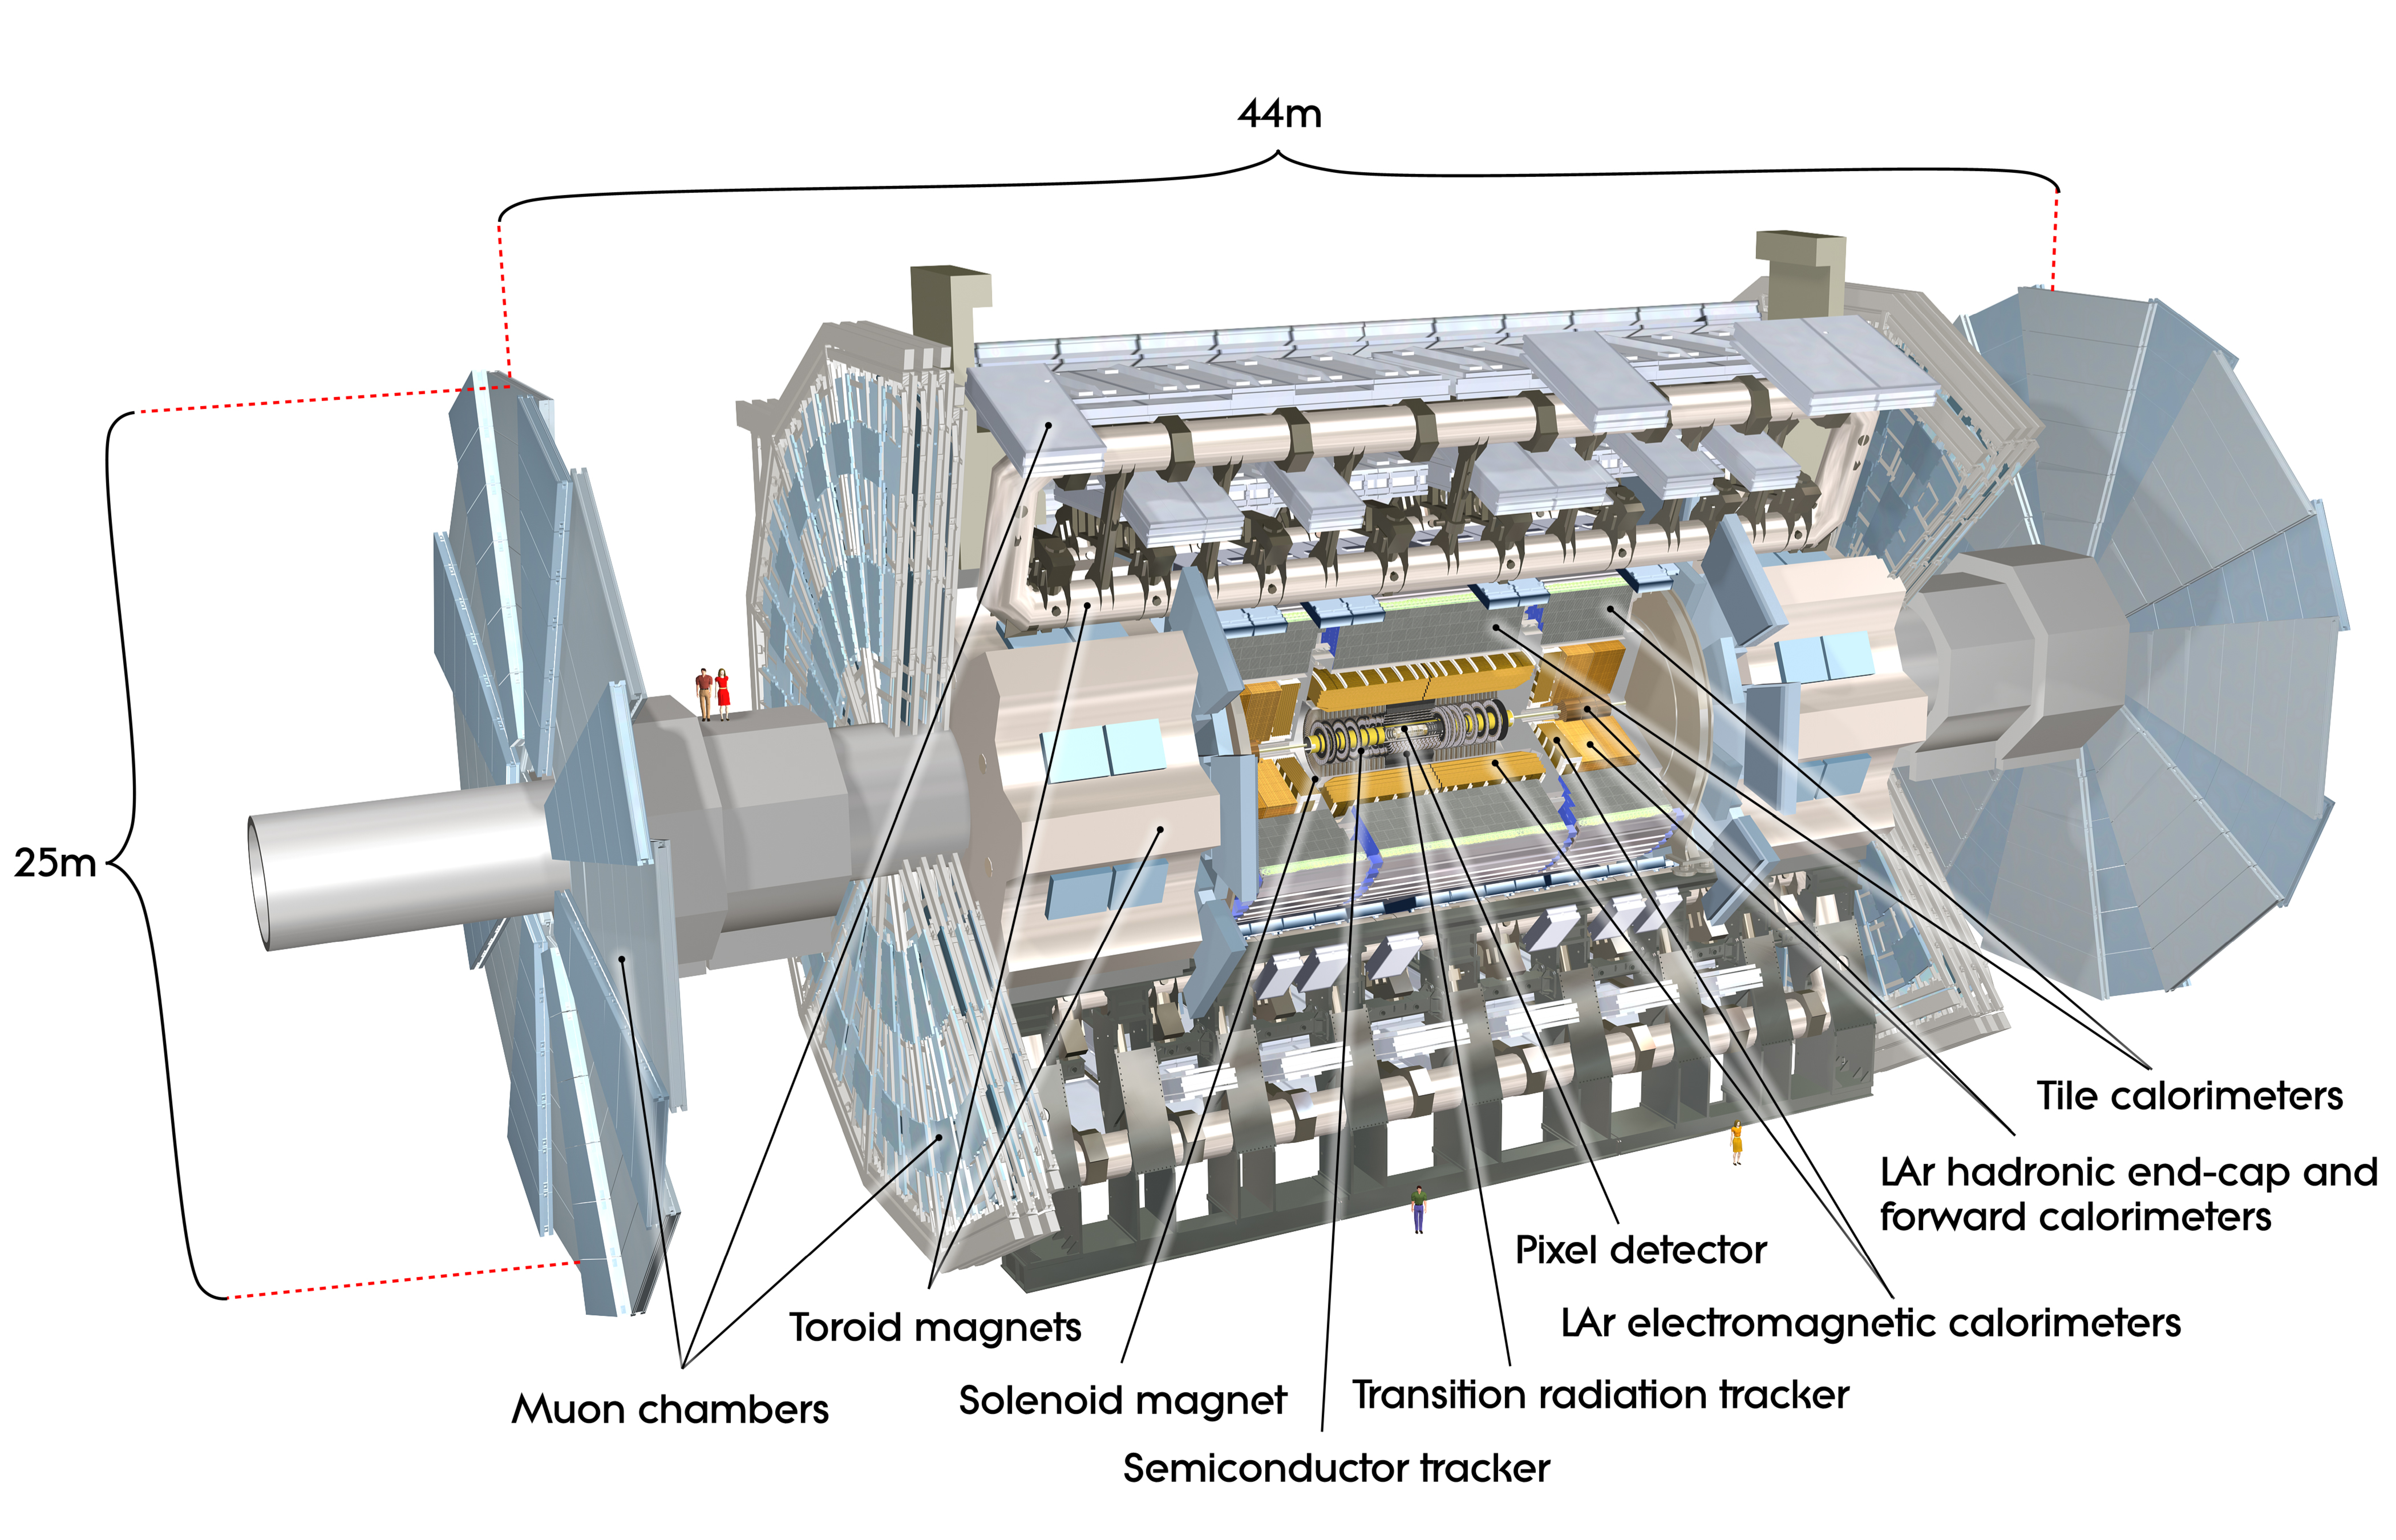
\includegraphics[width=125mm]{ATLAS_Detector_overview}

    \includegraphics[width=100mm]{ATLAS_ID}
  \end{center}
  \caption{An overview diagram of the ATLAS detector (top) and a diagram of the Inner Detector tracking systems (bottom).}
  \label{fig:ATLAS_overview}
\end{figure}

%\cite{CERN:images_overview}
%\cite{CERN:images_id}
\subsection{Inner Detector}

The Inner Detector (ID) is primarily a silicon based tracking system designed to reconstruct charged particle tracks down to a tranverse momentum ($p_{T}$) of $~0.5\, GeV$. It covers the full $\phi$ angle and provides tracking up to $|\eta|< 2.5$. It also provides some rudimentary particle identification via transition radiation.
 
%\subsubsubsection{Pixel Detector}
The Pixel Detector is the central most detector in ATLAS, situated just 50.5 mm away from the beam line in the inner most layer. It consists of three layers of silicon pixel modules in the central barrel, and five disk layers in the high $\eta$ end cap regions. The detector contains 1744 sensors, each with 47232 pixes with dimensions $50 \times 400~\mu m^2$. The detector is exposed to intense radiation and as such must be exteremely radiation hard to allow precision tracking measurements. During the first upgrade, the current pixel detector with be augmented with an additional layer, the insertable b-layer (IBL), to provide improved accuracy and vertex identification. 

%\subsubsubsection*{Semi Condictor Tracker (SCT)}
Continuing outwards from the Pixel Detector one encoutners the SCT. While also a silicon based technology, the SCT is a strip based detector rather than a pixel detector. Twi strips are places at small stero angles in 4 layers to allow for 4 individual space point measurements (in a total of 8 layers). The small stero angle (16 micro radians?) reduces the number of ambiguous space point solutions. When combined with the global position of the modules, a 3D space point can be constructed just as in the pixel detector, though the technology is cheaper and easier to scale to the large surface areas required by the SCT.

%\subsubsubsection*{Transition Radiation Tracker (TRT)}
The final part of the inner detector is the transition radiation tracker (TRT). Unlike the other two silicon based layers, this layer is designed from straw tube technology.

\subsection{The Calorimeter}
%\subsubsubsection*{Electron Magnetic Calorimeter (EMCalo)}
%\subsubsubsection*{Hadronic Calorimeter (HCal)}
%\subsubsubsection*{Forward Calorimeters}

\subsection{Magnet Systems}
%\subsubsubsection*{Solenoid}
%\subsubsubsection*{Toroid}

\subsection{Muon Systems}
%\subsubsubsection*{Monitored Drift Tubes (MDTs)}
%\subsubsubsection*{Resistive Plate Chambers (RPCs)}
%\subsubsubsection*{Cathode Strip Chambers (CSCs)}
%\subsubsubsection*{Thin Gap Chambers (TGCs)}

\subsection{Other detectors}
%\subsubsubsection*{Minium Bias Scintilator Tiles (MBTS)}
%\subsubsubsection*{Beam Conditions Monitor (BCM)}

\section{ATLAS Trigger System}
\subsection{Level 1, Level 2 and Event Filter}

\section{Object Identification and Reconstruction}

\subsection{Electrons}
\label{sec:electrons}
 Electrons are reconstucted in ATLAS by combining EM calorimeter showers with inner detector tracks. Due to the limitations in the tracker, electrons are only reconstructed at $\eta < 2.47$ with the crack regions excluded ($1.37 < |\eta_{cluster}| < 1.52$). Electrons are required to have a $E_{T(corrected)} > 25 \GeV~$ where $E_{T(corrected)} = E_{cluster} / cosh(\eta_{track})$. In addition strict cuts are placed on the calorimeter shower shapes to require a central energy maximum to distinguish electrons from other jet signatures. 

\subsection{Muons}
\label{sec:muons}
Muons in ATLAS are reconstructed using the 'muid' algorithm that matches inner detector tracks with tracks in the Muon spectrometer. These types of muons are so called 'combined' muons. Due to detector acceptence limitations muons may only be reconstructed with $\eta < 2.5$. In order to ensure that muons are selected in a stable plateau of trigger efficiency at \pt~ cut of greater than 20 \GeV~ is imposed. Backgrounds of prompt muons are dominated by heavy flavour decays. In order to supress these a combination of isolation cuts are used. The sum \pt~ of tracks inside a delta R cone of 0.3 must be less than 2.5 GeV and the sum \et~ of must be less than 4 \GeV~ in the same cone size\cite{ATLAS:Top_dilep_xsec}. The values for these isolation cuts were optimised to provide high efficiency regardless of pileup. Finally, muons that overlap with a selected jet within a delta R of 0.4 are rejected. 

Muons are triggered using two algorithms; mu18 and mu18medium. For earlier data periods with low pileup mu18 is used. This is changed to the medium algorithm in later periods in order to maintain the trigger unprescaled at high efficiency in the presence of high pileup.

(find plot of reco efficiency and trigger efficiency)

\subsection{Jets}
\label{sec:jets}
Try to summarise Jets at ATLAS in a way that doesn't become a thesis by itself! Algorithm used: anti $K_{T}$ with cone size of 0.4 (also 0.6 for some QCD studies). EM Scale calibrated, pileup supression using inner detector tracks. 

\subsection{Missing Energy}
\label{sec:met}
Put up the huge formula for the \etmiss and all of its components. Show the study of \etmiss resolution as a function of sumET. 

\subsection{Photons, Pions and other signatures}
Briefly mention about pion reconstruction (mainly for Tau signatures?), Photons (since they're the natural converse to Electrons) and any other signatures that you can think of.








\clearpage
\chapter{Trigger Efficiency and Data Quality Monitoring}
%\addcontentsline{toc}{chapter}{Trigger Efficiency and Data Quality Monitoring}

\section{Trigger Tracking}
\subsection{Inside-Out Algorithms}
\subsection{Outside-In Algorithms}
\subsection{Tracking for Physics objects}

\section{Trigger Efficiency}

\section{Data Quality Monitoring}

\section{New Tools for Efficiency Measurements}
\subsection{Tag and Probe for electron Efficiencies}

\clearpage
\chapter{Variables sensitive to Spin Correlation}
\label{chapter:Variables}

The spin information of the top quarks may be accessed directly via their decay particles. In the SM top quarks decay almost exclusively to W bosons and b quarks. The b quarks go on to form bjets that are observable in the detector, and the W bosons decay to either a lepton and neutrino, or a up and down type jet pair. \ttbar\ decays are classified based on the decay mode of the W boson (for which there are two in each event). If both W bosons decay leptonically then this is said to be the 'dilepton' channel, and this is the channel that is used for this study. If one of the W bosons decays hadronically and one leptonically then this is said to be the 'semi-leptonic' decay channel, and if both W's decay hadronically then this is said to be the 'all hadronic' channel.

An important property of each channel to consider is how much of the spin information from the \ttbar\ pair may be accessed via the decay particles. Table \ref{tab:alphas} shows the spin analysing power of each particle in the \ttbar\ decay. The charged leptons coming from the W boson decay carry the full spin information of the parent top quarks, and hence observables constructed with the two charged leptons in the dilepton channel have the highest sensitivity. The down type quark originating from the W bosons decay also has high spin analysing power however these are difficult to differentiate from the less sensitive up type jet from the same W, and hence the semi-leptonic channel loses some sensitivity. In previous results from the Tevatron, the principal disadvantage of the dilepton channel was it's limited statistics. Though the dilepton decay channel's branching ratio is only 20\% of the semi-leptonic channels, this is no longer a limiting factor due to the large statistics availible at the LHC. The dilepton channel is therefore the most sensitive channel for spin correlation analyses. 

The dilepton channel also offers experimental advantages over other channels. The signal for dilepton events is typically much cleaner than that for semi-leptonic, and with the addition of btagging requirements, backgrounds from other physics signals may be reduced to less than 10\% of the signal. 

The spin information for the top quarks can be readily accessed through the angular distributions of it's decay particles (equation \ref{equ:topdiffxsec}), and the majority of the observable exploit this fact. Equation \ref{equ:topdiffxsec} shows the top differential cross section, where $\theta_i$ is the angle of the charged lepton relative to the top helicity in the \ttbar\ rest frame, P is the polarisation of the top and $\alpha_i$ is the spin analysing power of the lepton. We can also construct the double differential cross section (\ref{eq:coscos}) where in this case we have assumed that the polarisation parameter, P, is equal to 1 and where $\sigma$ denotes the cross section of the channel under
consideration. $C$ is a free parameter between -1 and 1 that depends on the choice of the spin basis. At tree level in the SM, where the spin analysing power of the charged leptons is +1, $C=A$ represents the number of events where the $t$ and $\bar{t}$ spins are parallel minus the number of events where they are anti-parallel normalized by the total number of events:

\begin{equation}
    A = \frac{N_{like} - N_{unlike}}{N_{like} + N_{unlike}} =
     \frac{N(\uparrow \uparrow) + N(\downarrow \downarrow) - N(\uparrow \downarrow) - N(\downarrow \uparrow)}
     {N(\uparrow \uparrow) + N(\downarrow \downarrow) + N(\uparrow \downarrow) + N(\downarrow \uparrow)}.
    \label{eqno1}
\end{equation}
$\theta_+$ ($\theta_-$) describes the angle between
the direction of flight of the lepton $\ell^+$ ($\ell'^-$) in the \ttbar\ rest frame and a reference direction $\bf \hat{a}$ ($\bf\hat{b}$). The choice of spin basis determines the extent to which the spins of the top quarks are correlated. The choice of basis is discussed further in section \ref{sec:coscos}.

\begin{equation}
	\frac{1}{\sigma}\frac{d^2\sigma}{d[\cos{(\theta_i)}]d[\cos{(\theta_j)}]}= \frac{1}{4}[ 1 + \textcolor{Red}{\mathbf{P}}\textcolor{Green}{\boldsymbol{\alpha_i}}\cos{(\theta_i)} + \textcolor{Red}{\mathbf{P}}\textcolor{Green}{\boldsymbol{\alpha_j}}\cos{(\theta_j)} + \textcolor{blue}{\mathbf{A}}\textcolor{Green}{\boldsymbol{\alpha_i\alpha_j}}\cos{(\theta_i)}\cos{(\theta_j)}]
\end{equation}

\begin{equation}
	\begin{aligned}
	    	\textcolor{blue}{\mathbf{A}} &=\frac{N(\uparrow \uparrow) + N(\downarrow \downarrow) - N(\uparrow \downarrow) - N(\downarrow \uparrow)}{N(\uparrow \uparrow) + N(\downarrow \downarrow) + N(\uparrow \downarrow) + N(\downarrow \uparrow)} \\
		\textcolor{Green}{\boldsymbol{\alpha_{i/j}}} &= \text{\scriptsize{Spin Analysing Power of Analyser i/j}} \\
		\boldsymbol{\theta_{i/j}} &= \text{\scriptsize{Angle between Analyser and Basis}}\\
                \textcolor{Red}{\mathbf{P}} &= \frac{N(\cos(\theta_{i,j}) > 0) - N(\cos(\theta_{i,j}) < 0}{N(\cos(\theta_{i,j}) > 0) + N(\cos(\theta_{i,j}) < 0} \\
	\end{aligned}
\end{equation}

\begin{equation}
    \textcolor{Red}{\mathbf{P}} = \text{Polarisation of top/anti top}
\end{equation}

\begin{equation}
    \textcolor{Green}{\boldsymbol{\alpha_{i/j}}} = \text{Spin Analysing Power of lepton i/j}
\end{equation}

\begin{equation}
	A^{i}_{C} = \frac{N(\Delta |y^i| > 0) - N(\Delta |y^i| < 0)}{N(\Delta |y^i| > 0) + N(\Delta |y^i| < 0)}
\end{equation}

\begin{equation}
	\mathbf{P} = \frac{N(\cos(\theta_{l,n}) > 0) - N(\cos(\theta_{l,n}) < 0}{N(\cos(\theta_{l,n}) > 0) + N(\cos(\theta_{l,n}) < 0}
\end{equation}

\begin{equation}
	\begin{aligned}
	|\Delta y^i | &= |y^{t~~}| - |y^{\bar{t~~}}| \\
	                 &= |y^{l^{+}}| - |y^{l^{-}}| \\
	                 &= |\eta^{l^{+}}| - |\eta^{l^{-}}| \\
	\end{aligned}
\end{equation}


\begin{equation}
	\begin{aligned}
	A^{\l\l}_C &= 0.023 \pm 0.012 (stat.) \pm 0.008 (syst.) \\
	A^{\l\l}_C &= 0.004 \pm 0.001 (prediction)
	\end{aligned}
\end{equation}

\begin{equation}
	\begin{aligned}
	A^{t\bar{t}}_C &= 0.057 \pm 0.024 (stat.) \pm 0.015 (syst.) \\
	A^{t\bar{t}}_C &= 0.006 \pm 0.002 (prediction)
	\end{aligned}
\end{equation}



\begin{equation}
	\begin{aligned}
	A_{C}^{inclusive} &= -0.019 \pm 0.028~\text{(stat.)} \pm 0.024~\text{(syst.)} \\
	A_{C}^{high}       &= -0.052 \pm 0.070~\text{(stat.)} \pm 0.054~\text{(syst.)}~m_{t\bar{t}} < 450 GeV \\
	A_{C}^{low}         &= -0.008 \pm 0.035~\text{(stat.)} \pm 0.032~\text{(syst.)}~m_{t\bar{t}} > 450 GeV \\
	\end{aligned}
\end{equation}

%%%%%%%%%%%%%%%%%%%%%%%%%%%% equation %%%%%%%%%%%%%%%%%%%%%%%%%%%%%%                                                                                                             
\begin{equation}
\frac{1}{N} \frac{dN}{d \cos (\theta_i)} = \frac{1}{2} \left[1 + P \alpha_i \cos(\theta_i) \right],
\end{equation}
\label{equ:topdiffxsec}


\begin{equation}
\label{eq:coscos}
\frac{1}{\sigma} \frac{d\sigma}{d\cos\theta_+ d\cos\theta_-} =
\frac{1}{4} ( 1 - C \cos\theta_+ \cos\theta_- ) \,\, ,
\end{equation}

%%%%%%%%%%%%%%%%%%%%%%%%%%%%%%%%%%%%%%%%%%%%%%%%%%%%%%%%%%%%%%%%%%%%%%                                                                                                             

\begin{table}[htbp]
\begin{center}
\begin{tabular}{|c||c|c||c||c|c|}
\hline
%\BB \TT & $b$-quark & $W^+$ & $l^+$ & $\bar{d}$-quark or $\bar{s}$-quark& $u$-quark or $c$-quark\\
blah & $b$-quark & $W^+$ & $l^+$ & $\bar{d}$-quark or $\bar{s}$-quark& $u$-quark or $c$-quark\\
\hline
$\alpha_i$ (LO) & -0.41 & 0.41 & 1 & 1 & -0.31 \\
$\alpha_i$ (NLO) & -0.39 & 0.39 & 0.998 & 0.93 & -0.31 \\
\hline
\end{tabular}
\end{center}
\caption{Standard Model spin analysing power, at leading order and next-to-leading order 
for the decay products of the top quark from the decay $t \ra bW^+$.  The decay products of the $W$-boson 
can also be used as spin analysers, hence the decay products from leptonic decays 
$W^+ \ra l^+\nu_l$ and the hadronic decays $W \ra q_1\bar{q}_2$ are given in the table.  
Signs are reversed for a spin down top quark \cite{hubaut, Czarnecki:1990pe, Brandenburg:2002xr}.}
\label{tab:alphas}
\end{table}

\section{\dphi}
It has been shown in previous studies~\cite{mahlon2010,atlasspinprl} that the difference in the azimuthal angle between the two charged leptons in the dilepton decay is sensitive to spin correlations. This variable has important advantages to consider, particularly for the dilepton analysis. Firstly, it may be measured in the laboratory frame and hence does not require full \ttbar\ event reconstruction (which typically is not possible for all events). This production methods is the dominant mechanism at the LHC via gluon-gluon fusion. This suggests that the \dphi variable should show obvious differences between the SM spin case, and the no spin correlation case. Indeed this can be readily seen in figure \ref{fig:parton_dphi}.  These features make this variable ideal for observation of spin correlations~\cite{atlasspinprl}  however it is lacking in sensitivity in the quark-anti quark annihilation sector, where some new physics models are predicted to have observable effects.

An example of this variable is shown in figure \ref{fig:parton_dphi} showing \dphi with both SM spin correlations and no spin correlation. This variable has also been studied as a possible observation variable for light stop production in SUSY~\cite{lightstop}.

\begin{figure}[htpb!]
\begin{center}
%\includegraphics[width=75mm]{f/dilepton_delta_phi_7000}
%\includegraphics[width=50mm]{f/dilepton_delta_phi_400_7000}
\end{center}
\caption{Distribution of \dphi\ for parton level events at $\sqrt{s}=7$~TeV. The histogram shows the Standard Model and uncorrelated scenarios. }
%\caption{Distribution of \dphi\ for parton level events at $\sqrt{s}=7$~TeV (left) and with                                                                                       
%a cut requiring m(\ttbar) $< 400$~GeV (right).  The two histograms show the Standard Model and                                                                                    
%uncorrelated scenarios. An increase in the seperation between the two templates can be readily                                                                                    
%seen with the addition of an invariant mass cut.}      
\label{fig:parton_dphi}
\end{figure} 

\section{Angular correlation}
\label{sec:coscos}
Another variable directly correlated with the \ttbar\ spin correlation is \coscos. 
The double differential distribution for a measurement of  
spin correlations between $t$ and $\bar{t}$ is described in equation \ref{eq:coscos}. The degree of observable spin correlation is not fixed and a choice must be made to optimise the spin correlation parameter.
%
%%%%%%%%%%%%%%%%%%%%%%%%%%%%%% equation %%%%%%%%%%%%%%%%%%%%%%%%%%%%%%
%\begin{equation}
%\label{eq:coscos}
%\frac{1}{\sigma} \frac{d\sigma}{d\cos\theta_+ d\cos\theta_-} =
%\frac{1}{4} ( 1 - C \cos\theta_+ \cos\theta_- ) \,\, ,
%\end{equation}
%%%%%%%%%%%%%%%%%%%%%%%%%%%%%%%%%%%%%%%%%%%%%%%%%%%%%%%%%%%%%%%%%%%%%%
%
%where $\sigma$ denotes the cross section of the channel under
%consideration and $C$ is a free parameter between -1 and 1 that
%depends on the choice 
%of the spin basis. 
%%At tree level in the SM, where the spin analysing power of the charged
%leptons is +1, $C=A$ represents the number of events where the $t$ and
%$\bar{t}$ spins are parallel minus the number of events where they are
%anti-parallel normalized by the total number of events:
%\begin{equation}
%    A = \frac{N_{like} - N_{unlike}}{N_{like} + N_{unlike}} =
%     \frac{N(\uparrow \uparrow) + N(\downarrow \downarrow) - N(\uparrow \downarrow) - N(\downarrow \uparrow)}
%     {N(\uparrow \uparrow) + N(\downarrow \downarrow) + N(\uparrow \downarrow) + N(\downarrow \uparrow)}.
%    \label{eqno1}
%\end{equation}
%$\theta_+$ ($\theta_-$) describes the angle between 
%the direction of flight of the lepton $\ell^+$ ($\ell'^-$) in the $t$
%($\bar{t}$) rest frame and a reference direction $\bf \hat{a}$ ($\bf
%\hat{b}$). The choice of spin basis determines the extent to which the
%spins of the top quarks are correlated. 

\subsection{Beamline}
The \emph{beamline} basis takes the positive z axis direction~\footnote{The ATLAS coordinate system is right-handed with the
pseudorapidity, $\eta$ , defined as $\eta = −\ln[\tan(\theta/2)]$, where the
polar angle $\theta$ is measured with respect to the LHC beamline. The
azimuthal angle, $\phi$, is measured with respect to the x-axis, which
points towards the center of the LHC ring. The z-axis is parallel to
the anti-clockwise beam viewed from above. Transverse momentum and
energy are defined as $p_T =p \sin\theta$ and $E_T =E \sin\theta$, respectively.} as an approximation for the direction of one of the incoming protons. In this basis all information about the the spin correlation is lost. The expected value of the spin correlation strenght is $A = 0.03$. This is in contrast to the Tevatron collider, where the beamline basis can yield spin correlation values close to unity at leading order. In the following, we will not further investigate spin correlation in this basis. 

\subsection{Helicity}
The \emph{helicity} basis takes the direction of momentum of the top quark in the \ttbar rest frame, boosted into the top rest frame, as the spin analysing basis. This basis provides much better spin correlation strength, with $A=0.32$ at next to leading order~\cite{Bernreuther:2010ny}. 

\subsection{Optimised}
The \emph{optimised} basis is difficult to visualise conceptually but is derived mathematically from the spin density matrix of the \ttbar system. It can be thought of as interpolating between two other bases depending on the boost of the system. It is, by construction, the most sensitive variable that it is possible to construct at the LHC with a leading order spin correlation strength of $A=0.42$.

Since the angles described above require boosts into the top and anti-top rest systems, repsectively, a full reconstruction of the \ttbar system is required. For some events it is not possible to obtain a real solution for a given set of input parameters, regardless of the individual reconstruction algorithm that is applied. For this reason the cosine variables lose statistics in an already statistically limited channel (typically on the order of 10-15\%). It is fortunate that at the LHC dilepton top pairs are in adbundance and so this does not become a limiting factor.  

\section{Ratio Variables}

\subsection{R Ratio}
\subsection{S Ratio}

%One of the crucial advantages to these variables is that they are sensitive to the new physics models developed to explain the Tevatron \ttbar\ forward backward assymetry (cite D0 and CDF). This feature may be enhanced by requiring a high \ttbar\ invariant mass, as this biases the ratio of gluon-gluon fusion to qqbar anihilation towards the qqbar, where most of these BSM models exist.

\clearpage
\chapter{Event Reconstruction}

\section{Data Sample}

During 2011 the LHC delivered over 5.6 fb$^{-1}$ of integrated luminosity to ATLAS at a centre of mass energy of 7 TeV. Approximately 5.25 fb$^{-1}$ of this was recorded and, after data quality considerations, resulted in 4.665 fb$^{-1}$ of analysable data at a peak instantaneous luminosity of 3.65 * 10$^{33}$~cm$^{-2}$s$^{-1}$. The 7 TeV run period was divided into sections corresponding to stable conditions, fixed instantaneous luminosity and bunch configuration; called periods. There were 13 periods in the 2011 data, labelled period A - period M. Some periods did not have stable detector conditions and as such are not considered in physics analyses, for example period A.

\begin{figure}[htbp!]
\begin{center}
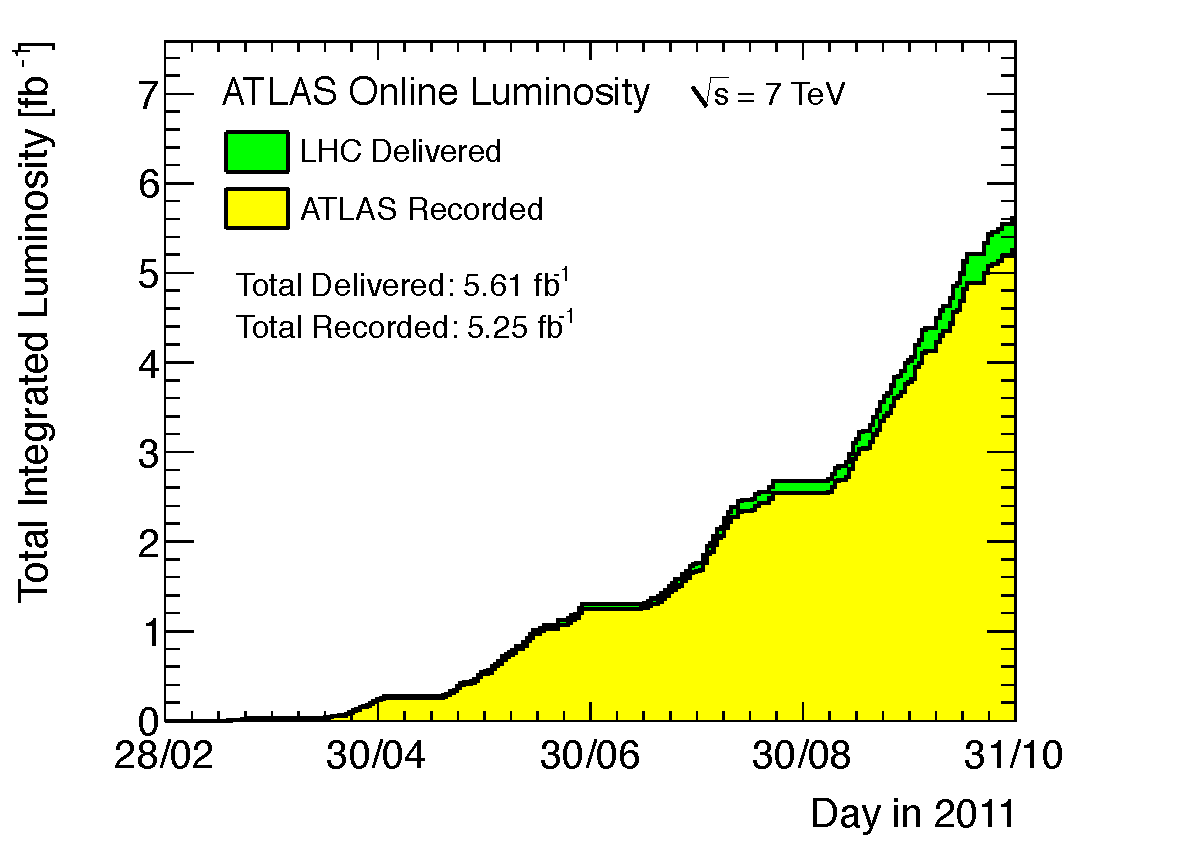
\includegraphics[width=75mm]{f/sumLumiByDay}
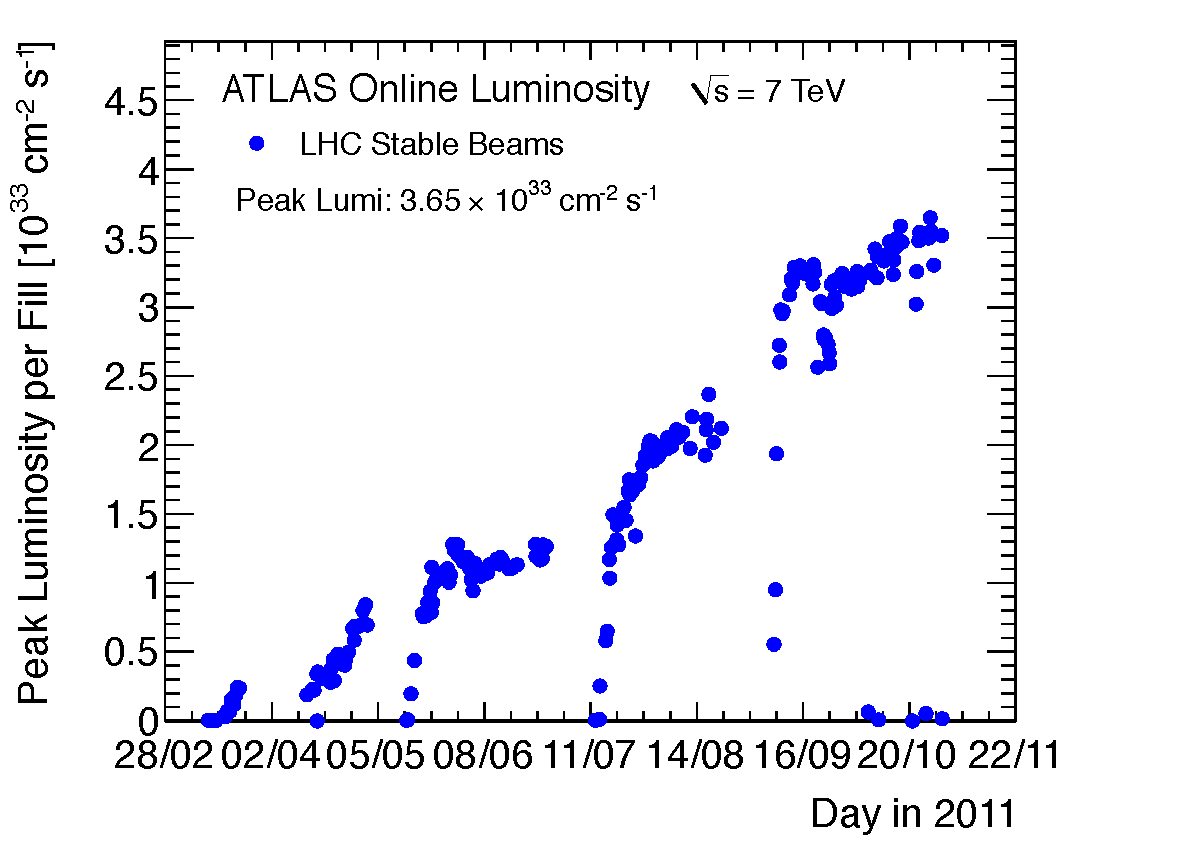
\includegraphics[width=75mm]{f/peakLumiByFill}
\end{center}
\caption{ATLAS integrated luminosity during 2011 \textit{(left)}. Peak instantaneous luminosity during the LHC7 run recorded by ATLAS \textit{(right)}.}
\label{fig:lumi}
\end{figure}

\section{Analysis Triggers}
\label{sec:analysis_trigger}

To select interesting \ttbar\ like events with high efficiency we use triggers based on single electron or muon signatures. Lepton signatures are plentiful in 7 TeV proton-proton collisions and in order to reduce the trigger rate to a manageable level it is necessary to impose a minimum \pt\ threshold on the trigger lepton. Electron triggers were required to have a trigger electron with minimum \pt\ of 20 GeV in periods B-J, a minimum \pt\ of 22 GeV in period K and either 22 GeV or 45 GeV in periods L-M, depending on other cuts in the trigger. The higher threshold of 45 GeV is used to accept events that are rejected by the lower threshold trigger in periods L-M. For muons a minimum \pt\ cut of 18 GeV is required in all periods.

In addition to \pt\ requirements, other cuts can be made to reduce trigger rate. For electrons these are based on calorimeter cluster information and inner detector trigger track isolation. For muons these are based on Muon Spectrometer trigger track isolation and other track quality parameters. Triggers at ATLAS have the definition of either \emph{loose}, \emph{medium}, or \emph{tight} depending on their efficiency. \emph{Loose} triggers have high efficiency but low background rejection (or ``purity"), whereas \emph{tight} triggers have lower efficiency but higher purity.~\emph{Medium} triggers attempt to balance efficiency with purity and are the triggers used in this analysis. In addition other affixes in the trigger name indicate a unique or unusual cut that is not always applied. For example in table \ref{tab:analysis_triggers}, the letters \emph{vh} in the electron triggers indicate that this trigger applied $\eta$ dependent cuts on hadronic isolation at trigger L1 \cite{LeptonTrigger}.

\begin{table}
	\begin{center}
	\begin{tabular}{|c|c|c|c|}
	\hline
	Data period & Int. Luminosity & Electron Trigger & Muon Trigger \\
	\hline
	period B-D    & $0.176~$fb$^{-1}$  & EF\_e20\_medium     & EF\_mu18        \\
	period E-H    & $0.938~$fb$^{-1}$  & EF\_e20\_medium     & EF\_mu18        \\
	period I      & $0.333~$fb$^{-1}$  & EF\_e20\_medium     & EF\_mu18        \\	
    period J      & $0.223~$fb$^{-1}$  & EF\_e20\_medium     & EF\_mu18\_medium\\
	period K      & $0.583~$fb$^{-1}$  & EF\_e22\_medium     & EF\_mu18\_medium\\
	period L-M    & $2.402~$fb$^{-1}$  & EF\_e22vh\_medium1 OR EF\_e45\_medium1     & EF\_mu18\_medium\\
	\hline
	\end{tabular}
	\end{center}
	\caption{Table of analysis triggers used for data taking in the 7 TeV data. Note that \emph{medium1} and \emph{medium} are two distinct triggers.}
	\label{tab:analysis_triggers}
\end{table}


\section{Event Selection}
\label{sec:event_selection}

Kinematic cuts and data quality requirements are imposed on the data and MC samples in order to optimise the signal to background ratio (i.e. to bias the sample towards the signal events and reject background events). A list of the cuts employed, along with the motivation for these cuts follows. 

\subsection*{Selection}
\begin{itemize}

  \item \textbf{Passed single lepton trigger}: Events are required to have fired either an electron or muon trigger, as described in section \ref{sec:analysis_trigger}.

  \item \textbf{Exactly two opposite sign leptons}: Exactly two well reconstructed leptons are required; either two electrons, two muons or one electron and one muon. All lepton pairs are must have opposite sign charge.

  \item \textbf{Two or more selected jets}: We require at least two well reconstructed jets in each event, though these need not be tagged as having b-flavour. When combined with the lepton multiplicity requirement, this cut removes most other SM physics signals from the selection, particularly in the \emu channel where there are no significant Drell-Yan contributions. Many background signals require extra radiated jets either from pileup or NLO radiative corrections in order to imitate the signal kinematics and therefore this cut is highly efficient at accepting signal events whilst reducing background signals, as can be seen in figures \ref{fig:dilep_control_sig_ee}, \ref{fig:dilep_control_sig_mumu} and \ref{fig:dilep_control_sig_emu}.

  \item \textbf{\etmiss $>$ 60 \GeV}: (\ee\ and \mumu\ channels only) This kinematic cut reduces contribution from Drell-Yan events (where there are no neutrinos is the hard scatter to create missing energy) and some diboson events by requiring a large amount of missing transverse energy. For \ttbar\ dilepton events the efficiency of this cut is very high due to the two neutrinos in the dilepton final state, illustrated in figures \ref{fig:dilep_control_sig_ee}, \ref{fig:dilep_control_sig_mumu}. This cut is not motivated in the \emu\ channel.

  \item \textbf{Invariant mass $>$ 15 \GeV}: (\ee\ and \mumu\ channels only)  Invariant mass is defined as the invariant mass between the two selected leptons in the event. Low energy Drell-Yan events and meson production such as $J/\Psi$ can enter the selection by decaying to two opposite sign leptons but typically have a low invariant mass and are rejected by this cut. The invariant mass of the \ttbar\ system tends to peak at much higher values and so this does not have a damaging effect on signal acceptance. This is shown in figures \ref{fig:dilep_control_sig_ee} and \ref{fig:dilep_control_sig_mumu}. 

  \item \textbf{$H_T >$ 130 \GeV }: (\emu\ channel only) $H_T$ is defined as the scalar sum of the transverse energy of all selected leptons and jets in the event. This cut is only applied in the \emu\ channel and can loosely be describe as requiring a large amount of energetic activity in the event. This cut rejects events with lower energy (for example a diboson event whose extra radiated jets are low in energy but still pass the jet $p_T$ cut.

  \item \textbf{Z Boson Veto }: (\ee and \mumu channels only) Events with an invariant mass that is less than 10 GeV away from the Z boson pole mass of 91 GeV are rejected. This cut reduces a large amount of the Drell-Yan $\rightarrow \ee$ or \mumu\ background. Events in which Z Bosons decay to two tau leptons (that then decay leptonically) have a broad invariant mass spectrum that peaks at lower values, illustrated in figures \ref{fig:dilep_control_sig_ee} and \ref{fig:dilep_control_sig_ee}, and a similar cut to suppress this background would result in an unacceptable loss of signal statistics. This cut also has difference acceptance in the standard model spin sample and the uncorrelated spin sample. This reason for this is that in the uncorrelated sample, the leptons typically have a larger separation in $\phi$ and hence a higher invariant mass. The efficiency of this cut is higher for the uncorrelated sample than it is for the standard model sample, but this effect is accounted for in the extraction procedure later and is typically small (on the order of 3\%).

In the dominant channel for dilepton events (the \emu\ channel), there are no cuts on invariant mass as there are no standard model processes where Z Bosons may violate lepton flavour conservation and decay to an electron and a muon.

  \item \textbf{Cosmic Rejection}: Events are rejected if two muon tracks are back to back in phi (i.e. $\Delta\phi > 3.1$) and if the point of closest approach to the vertex is greater than 5mm, with both tracks on the same side of the detector. 

  \item \textbf{Data Quality Cuts}: An event in data is required to have been included in a good run list (GRL). These GRLs are generated centrally by ATLAS and reject events where data quality was deemed to be poor by experts. Physics subgroups may impose their own requirements if appropriate. In the case of a predominantly jet based analysis, bad data quality the inner detector may be a tolerable defect, whereas for a muon based Drell-Yan selection the calorimeter information may not be necessary. For top analyses we require that the entire detector is online and that the data quality has been assessed to be good by the relevant experts (see section \ref{sec:dq}).

A reconstructed vertex with at least three tracks is required to have been identified as a primary vertex and not originating from pileup. 

In 2011 a tower of the ATLAS Liquid Argon calorimeter was disabled creating a hole in the acceptance. In the portions of effected data, events are rejected where it is believed that a jet has been mismeasured due to this fault. In addition the effect of this is taken into account in the detector simulation and reconstruction of \etmiss .

  \item \textbf{Passed Truth Cuts}: In signal MC events, we require that the selected event be a true dilepton \ttbar\ event, and that the two reconstructed leptons correspond to the true leptons for this event and are not from a secondary process (such as a semi-leptonic b decay). This avoids double counting contributions from mismeasured leptons, which are estimated separately using a data driven method. 

\end{itemize}

With the application of all cuts the contribution of background to the selection is approximately 20\%. With the addition of a single b-jet requirement (b-tag) this can be reduced to 10\%, with only single top events being an effective background. The cost in statistics for utilizing b-tagging  to signal events is quite large (on the order of $~20$\%). Though the 7 TeV has ample statistics in dileptonic \ttbar\ events, the cut effectively removes the \ee\ channel as a useful dataset and so it is not included in the final selection. For future results with higher statistics and higher centre of mass energies it may prove useful to impose a double b-tag, which effectively removes most SM background events. 

\subsection{Signal Monte Carlo}
Signal \ttbar\ events are generated using the MC@NLO generator interfaced with HERWIG and JIMMY for parton showering (PS) and underlying event (UE) simulation respectively. MC@NLO generates both top quarks, the W and b particles, and the subsequent W decay. HERWIG then showers the b quarks and W boson daughters (in the dilepton case electrons, muons or taus). By adjusting the point at which HERWIG initiates the showering and decay, spin correlation can effectively be removed from the MC. If HERWIG is allowed to decay the top quarks then they will be treated as unpolarised and uncorrelated. In this manner we generate 15 million \ttbar\ events with spin correlation (semi-leptonic and dileptonic) and 10 million events without spin correlation (again without fully hadronic decays). This technique has the side effect of the top quarks in the uncorrelated case being treated as on shell and hence not including an intrinsic width. The effect of this is describe further in section \ref{sec:systematics} and is estimated to be negligible.

Signal events are also generated with POWHEG interfaced to HERWIG or PYTHIA, as well as ALPGEN interfaced to HERWIG; all using JIMMY for UE modelling. These samples are only used for the estimation of systematic uncertainties.

Care must be taken when interfacing HERWIG with different ME generators. In certain combinations HERWIG will not pass tau polarisation information correctly\footnote{Tau decays in HERWIG are handled by the TAUOLA program.} and tau decays will be treated as unpolarised, effectively making an event with a tau decay appear uncorrelated. This was noted in all ATLAS MC samples and is only present in the POWHEG + HERWIG implementation. This is discussed further in section \ref{sec:systematics}. In a similar analysis performed by CMS, this was not accounted for in the signal MC and became a dominant source for systematic uncertainty.  

Fully hadronic \ttbar\ decays are not considered in our samples as these events can only contribute to the selection via non prompt leptons and hence fall under the definition of an experimentally mismeasured lepton events. 

\subsection{Data driven background estimation}

Ideally one would prefer to estimate as many background processes as possible using data driven techniques as these suffer less from theoretical uncertainties than estimations base on MC alone. In this selection the normalisation of Drell-Yan MC is derived by comparing the normalisation of the MC with data in a Drell-Yan dominated control region. Experimentally mismeasured leptons, or ``fake'' leptons as they are more commonly known, are also estimated using a data driven technique. These are defined as leptons arising from photon conversions, mismeasured jets (as electrons) and leptons arising from heavy flavour decays inside jets. Leptons arising from hard scatter leptonic tau decay are not considered as fakes. 

\subsubsection*{Matrix Method for determining fake lepton background}

The matrix method is used to determine the shape and normalisation of backgrounds due to fake leptons \cite{fakes}\cite{topwg}. It's goal is to use measurable quantities, such as the rate at which a reconstructed lepton passes isolation cuts, to estimate the number of fake leptons contaminating the data selection. It defines two lepton definitions, \emph{loose} and \emph{tight}. The \emph{tight} selection is the selection used for analysis (see section \ref{sec:electrons},~\ref{sec:muons}), the \emph{loose} selection is the same as the \emph{tight} selection but with isolation requirements relaxed (in the case of electrons) or removed (in the case of muons). The number of loose and tight leptons are quantities that may be observed in data.

We define two efficiencies, derived from MC; one for fake leptons and one for real leptons (i.e. prompt hard scatter) such that:

\begin{equation}
	\textcolor{Blue}{\mathbf{r_i}} = \epsilon_{real} = \frac{  N^{\text{tight}}_{\text{real}} }{ N^{\text{loose}}_{\text{real}} }~~~~\&~~~~\textcolor{Red}{\mathbf{f_i}} = \epsilon_{\text{fake}} = \frac{ N^{\text{tight}}_{\text{fake}} }{ N^{\text{loose}}_{\text{fake}}}
	\label{eq:fake_eff}	
\end{equation}

The $\epsilon_{real}$ is measured using a tag and probe technique in Z boson events, and the $\epsilon_{fake}$ is measured from control regions with high contributions from fake leptons, for example a same sign low \etmiss\ selection. The number of events with different lepton quality definitions may then be expressed in matrix form:

\begin{equation}
\begin{bmatrix}
%N^{\textcolor{blue}{\mathbf{tt}}} \\
%N^{\textcolor{blue}{\mathbf{t}}\textcolor{red}{\mathbf{l}}} \\
%N^{\textcolor{Red}{\mathbf{l}}\textcolor{blue}{\mathbf{t}}} \\
%N^{\textcolor{Red}{\mathbf{ll}}} \\
N^{\mathbf{tt}} \\
N^{\mathbf{t}\mathbf{l}} \\
N^{\mathbf{l}\mathbf{t}} \\
N^{\mathbf{ll}} \\
\end{bmatrix} 
= \mathbf{M}
\begin{bmatrix}
%N^{\textcolor{Red}{\mathbf{ll}}}_{\textcolor{Green}{\mathbf{rr}}} \\
%N^{\textcolor{Red}{\mathbf{ll}}}_{\textcolor{Green}{\mathbf{r}}f} \\
%N^{\textcolor{Red}{\mathbf{ll}}}_{fr} \\
%N^{\textcolor{Red}{\mathbf{ll}}}_{ff} \\

%N^{\mathbf{ll}}_{\textcolor{Blue}{\mathbf{rr}}} \\
%N^{\mathbf{ll}}_{\textcolor{Blue}{\mathbf{r}}\textcolor{Red}{\mathbf{f}}} \\
%N^{\mathbf{ll}}_{\textcolor{Red}{\mathbf{f}}\textcolor{Blue}{\mathbf{r}}} \\
%N^{\mathbf{ll}}_{\textcolor{Red}{\mathbf{ff}}}\\

N^{\mathbf{ll}}_{\rone\rtwo}\\
N^{\mathbf{ll}}_{\rone\ftwo}\\
N^{\mathbf{ll}}_{\fone\rtwo}\\
N^{\mathbf{ll}}_{\fone\ftwo}\\
\end{bmatrix}
\label{eq:fake}
\end{equation}

\begin{equation}
\mathbf{M} = 
\begin{bmatrix}
%r_1 r_2         & r_1f_2         & f_1r_2         & f_1f_2 \\
%r_1(1-r_2)     & r_1(1-f_2)     & f_1(1-r_2)     & f_1(1-f_2) \\
%(1-r_1)r_2     & (1-r_1)f_2     & (1-f_1)r_2     & (1-f_1)f_2 \\
%(1-r_1)(1-r_2) & (1-r_1)(1-f_2) & (1-f_1)(1-r_2) & (1-f_1)(1-f_2) \\

\rone \rtwo          & \rone \ftwo         & \fone \rtwo         & \fone \ftwo \\
\rone (1-\rtwo )     & \rone (1-\ftwo )    & \fone (1- \rtwo )   & \fone (1- \ftwo ) \\
(1-\rone )\rtwo      & (1-\rone )\ftwo     & (1-\fone )\rtwo     & (1-\fone )\ftwo  \\
(1-\rone )(1-\rtwo ) & (1-\rone )(1-\ftwo )& (1-\fone )(1-\rtwo )& (1-\fone )(1-\ftwo )\\

%(1-r_1)(1-r_2) & (1-r_1)(1-f_2) & (1-f_1)(1-r_2) & (1-f_1)(1-f_2) \\
\end{bmatrix}
\end{equation}

Where $N$ is the number of events passing the selection. The upstairs notation indicates the tightness of the selection (t = \emph{tight}, l = \emph{loose}) for each lepton, and the downstairs notation is if the lepton was real or fake. For the estimate of the fake contribution to the signal region we are interested in determining the number of events with at least one fake lepton contaminating the $N^{\mathbf{tt}}$ selection using observable properties such as the real and fake efficiencies for leptons, and the number of events with leptons passing \emph{tight} or \emph{loose} selections in data. We may extract this by inverting the matrix M and rearranging equation \ref{eq:fake} such that:

\begin{align}
N^{tt}_{fake} =&~ N^{tt}_{rf} + N^{tt}_{fr} + N^{tt}_{ff} \\
              =&~ \rone \ftwo N^{ll}_{rf} + \fone \rtwo N^{ll}_{fr} + \fone \ftwo N^{ll}_{ff} \\
              =&~ \alpha \rone \ftwo [(\fone -1)(1-\rtwo )N^{tt} + (1-\fone )\rtwo N^{tl} + \fone (1-\rtwo )N^{lt} - \fone \rtwo N^{ll}] \nonumber \\
               +&~ \alpha \fone \rtwo [(\rone -1)(1-\ftwo )N^{tt} + (1-\rone )\ftwo N^{tl} + \rone (1-\ftwo )N^{lt} - \rone \ftwo N^{ll}] \nonumber \\
               +&~ \alpha \fone \ftwo [(1-\rone )(1-\rtwo )N^{tt} + (\rone - 1)\rtwo N^{tl} + \rone (\rtwo  -1)N^{lt} + \rone \rtwo N^{ll}]
%              =&~ r_1f_2N^{ll}_{rf} + f_1r_2N^{ll}_{fr} + f_1f_2N^{ll}_{ff} \\
%              =&~ \alpha r_1f_2[(f_1-1)(1-r_2)N^{tt} + (1-f_1)r_2N^{tl} + f_1(1-r_2)N^{lt} - f_1r_2N^{ll}] \nonumber \\
%               +&~ \alpha f_1r_2[(r_1-1)(1-f_2)N^{tt} + (1-r_1)f_2N^{tl} + r_1(1-f_2)N^{lt} - r_1f_2N^{ll}] \nonumber \\
%               +&~ \alpha f_1f_2[(1-r_1)(1-r_2)N^{tt} + (r_1 - 1)r_2N^{tl} + r_1(r_2 -1)N^{lt} + r_1r_2N^{ll}]
\end{align}

where

\begin{equation*}
\alpha = \frac{1}{(\rone - \fone )(\rtwo -\ftwo )}
%\alpha = \frac{1}{(r_1 - f_1)(r_2-f_2)}
\end{equation*}

We can now extract $N^{\mathbf{tt}}$, $N^{\mathbf{tl}}$, and $N^{\mathbf{ll}}$ from the data in our signal selection and use our derived real and fake efficiencies to estimate the contributions from fake leptons. In practice this can be applied not as just single numbers but as distributions (such as our observable distributions) and the efficiencies may be parametrised as functions of $\eta$, $p_T$ or $\Delta R$ with closest jet. This method requires that $\epsilon_{fake}$ and $\epsilon_{real}$ are different, or at least the definitions of of tight and loose are different, and therefore care must be taken to maintain this assumption whilst maintaining a reasonable lepton definition.

\subsubsection*{Normalisation of Drell-Yan MC using data}
\label{sec:drell_yan}

In the \ee\ and \mumu\ channels the shape of background contributions from \Zee\ or \Zmm\ events is taken from Monte Carlo. The normalisation is taken by comparing data events to MC events in a region dominated by \Zll\ events using equation \ref{eq:drell_yan}. In this control region (CR) non Drell-Yan background (including \Ztautau\ ) are subtracted from the data to approximate the number of \Zee\ or \Zmm\ events seen in data. DIstributions in this control region are shown in figures \ref{fig:ee_control_dy} and \ref{fig:mumu_control_dy}.

 \begin{equation}
   \label{eq:drell_yan}
   N_{Z/\gamma^* + jets} = \frac{Data^{(CR)} - MC_{other}^{(CR)}}{MC_{Z/\gamma^* + jets}^{(CR)}} \times MC_{Z/\gamma^* + jets}^{(SR)}
 \end{equation} 

 \begin{table}[htb]
   \begin{center}
     \begin{tabular}{|c|c|c|}
       \hline
       Process & \ee & \mumu \\
       \hline
       Data (CR)         &  3170.0 & 9194.0  \\
       MC$_{DY}$ (CR)    &  2741.6 & 7586.0  \\
       MC$_{Other}$ (CR) &   374.2 &  711.8  \\
       \hline
       Scale Factor      &    1.02 &   1.12  \\
       MC$_{DY}$ (SR)    &    20.6 &  74.6   \\
       Scaled MC         &    21.0 &  83.5   \\
       \hline
     \end{tabular}
   \end{center}
   \caption{Yields for the estimates of the $Z/\gamma^*$+jets background
     with the data-driven and Monte Carlo methods using non-isolated electron fakes. Yields are shown in the Z dominated control region (CR) and in the signal region (SR).} %and total uncertainties
   \label{tab:dilep_znorm}
 \end{table}

\subsection{Monte Carlo background contributions}

\begin{figure}[htbp!]
\begin{center}
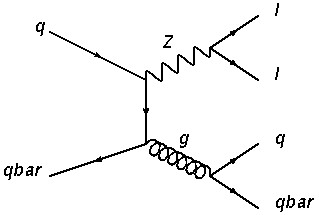
\includegraphics[width=75mm]{f/Z_jets}
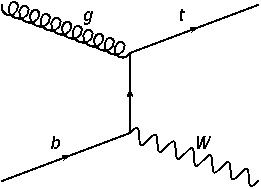
\includegraphics[width=65mm]{f/single_top_Wt}
\end{center}
\caption{Feynman diagrams of some of the dominant background SM processes to dileptonic \ttbar\ events; Z + jets \emph{(left)} and single top quark production \emph{(right)}}
\label{fig:background_feynman}
\end{figure}

Backgrounds that cannot be derived directly or indirectly from the data are determined from Monte Carlo samples. Events coming from single top production are modelled using MC@NLO interfaced with HERWIG and JIMMY. Only the associated production channel (Wt channel) is considered as only this can imitate the signal events without the addition of a fake lepton. 

Drell-Yan events are generated using the leading order generator ALPGEN interfaced to HERWIG and JIMMY for PS and UE respectively. Events are simulated with 0 - 5 (incl.) additional partons in both the high invariant mass regime (40 $\rightarrow$ 2000 GeV) and the low invariant mass regime (between 10 $\rightarrow$ 40 GeV). For dielectron and dimoun events the normalisation is derived from data (see section \ref{sec:drell_yan}). For ditau events, the normalisation is taken from the cross section used in the MC generator.

Events from dibosonic processes (WW, WZ, ZZ) are also modelled using ALPGEN + HERWIG/JIMMY. In these cases events are generated with 0, 1, 2 or 3 (inc.) additional partons. Each background sample derived from pure MC has an associated systematic uncertainty on the cross section. This is described further in section \ref{sec:systematics}.

\section{Selection on 7 TeV data}

Figures \ref{fig:ee_control_dy} to \ref{fig:dilep_lep2_emu} show comparisons between simulated events and observed events in the signal region and background dominated control regions. Good agreement is observed in all distributions. The uncertainty on the normalisation of the simulated samples is also shown. The procedure for estimating this uncertainty is described in section \ref{sec:systematics}. A small deviation in the jet multiplicity distribution at four or more jets is observed in the signal region. The cause of this was found to be the MC@NLO generator used to simulate the signal \ttbar\ events. MC@NLO underestimated the number of jets in the signal events causing the observed discrepancy. The problem is largely one of normalisation and significant changes in the shapes of distributions due to this effect are not observed. The observed yields in data and MC are summarised in table \ref{tab:dilep_cutflow}.

The \emu\ channel has the highest selection statistics, followed by \mumu\ and finally the \ee\ channel. The \ee\ and \mumu\ channel have cuts to supress Drell-Yan background that are not needed in the \emu\ channel and hence have lower statistics. The \ee\ channel has much lower statisics than the \mumu\ channel as the isolation cuts for electrons are much tighter than those for muons in order to suppress fake electrons.

\begin{table}[htbp!]
     \begin{center}
     \begin{tabular}{c c c c}
     \hline
      & \ee & \mumu & \emu \\
     \hline
     $Z+$jets (DD)                        &  21.0 &   83.5 &  -     \\
     $Z(\rightarrow \tau \tau)$+jets (MC) &  18.5 &   68.4 &  175.3 \\
     Fake leptons (DD)                    &  26.2 &   29.0 &  100.8 \\
     Single top (MC)                      &  31.2 &   84.0 &  228.5 \\
     Diboson (MC)                         &  22.9 &   61.4 &  177.6 \\
     \hline
     Total (non-\ttbar)                   & 119.8 &  326.3 &  622.2 \\
     \ttbar\ (MC)                         & 578.3 & 1668.0 & 4413.6 \\
     \hline
     Expected                             & 698.1 & 1994.3 & 5095.8 \\
     Observed                             & 740   & 2058   & 5328   \\
     \hline
     \end{tabular}
     \end{center}
     \caption{Observed events in Data and MC in the dilepton \ttbar\ selection. Backgrounds estimated from Monte Carlo are indicated with the (MC) suffix, whereas backgrounds estimated by data driven techniques are indicated with a (DD) suffix.}
     \label{tab:dilep_cutflow}
     \end{table}

\begin{figure}[hbtp!]
	 \begin{center}
         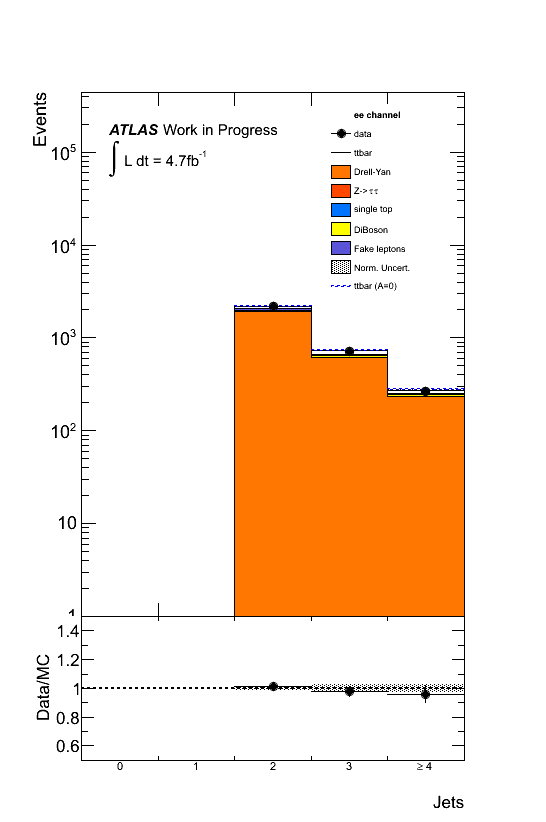
\includegraphics[width=50mm]{f/ee_dy_njet_central_double}
         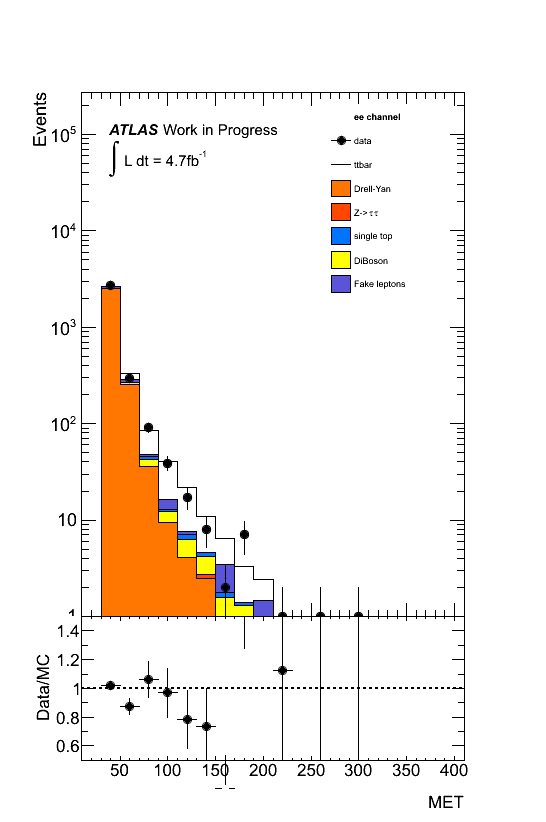
\includegraphics[width=50mm]{f/ee_dy_met_central_double}
         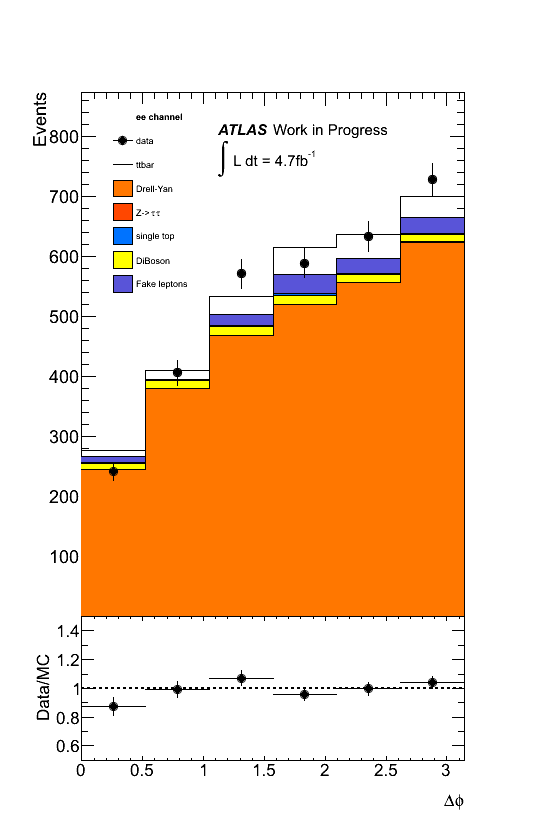
\includegraphics[width=50mm]{f/ee_dy_delta_phi_central_double}
       \end{center}
       \caption{Distributions for the \ee\ channel showing the jet multiplicity, reconstructed Z boson $p_{T}$, and $\Delta\phi$ analysis variable in the Drell-Yan control region.}
     \label{fig:ee_control_dy}
\end{figure}

\begin{figure}[hbtp!]
	 \begin{center}
         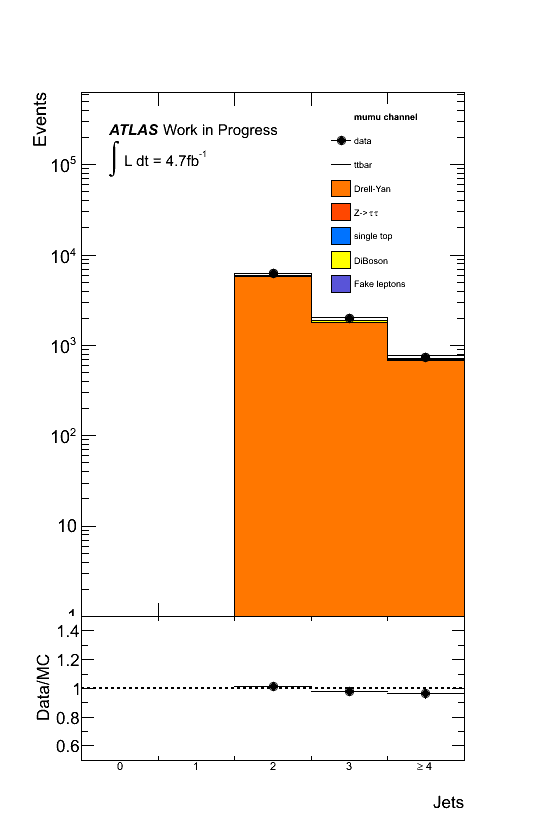
\includegraphics[width=50mm]{f/mumu_dy_njet_central_double}
         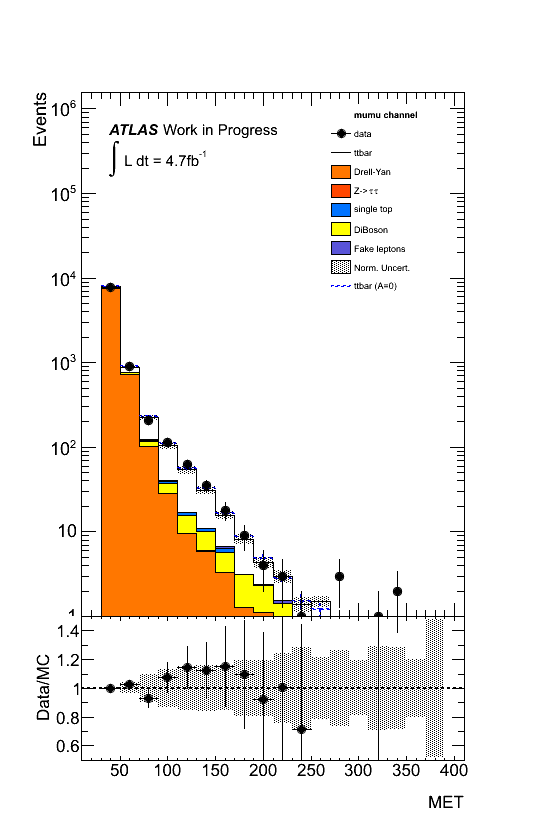
\includegraphics[width=50mm]{f/mumu_dy_met_central_double}
         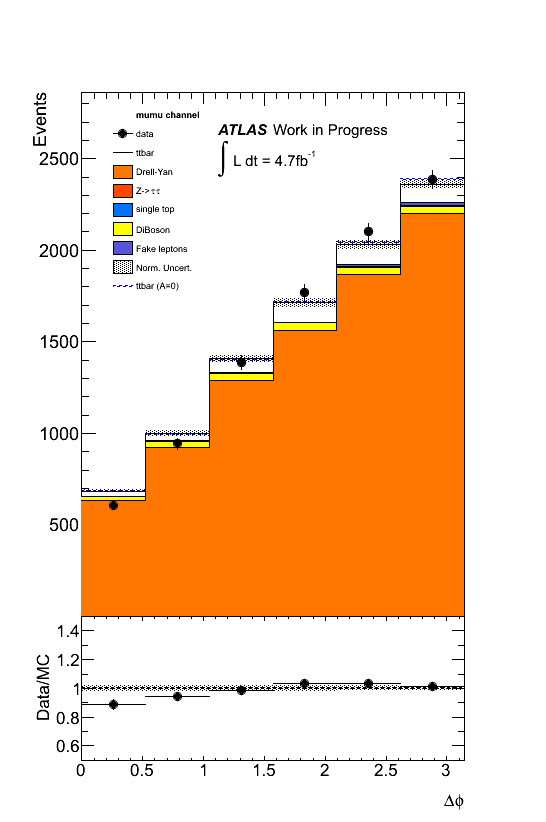
\includegraphics[width=50mm]{f/mumu_dy_delta_phi_central_double}
       \end{center}
       \caption{Distributions for the \mumu\ channel showing the jet multiplicity, reconstructed Z boson $p_{T}$, and $\Delta\phi$ analysis variable in the Drell-Yan control region.}
     \label{fig:mumu_control_dy}
\end{figure}
    
%     \begin{figure}[htbp!]
%     \begin{center}
%     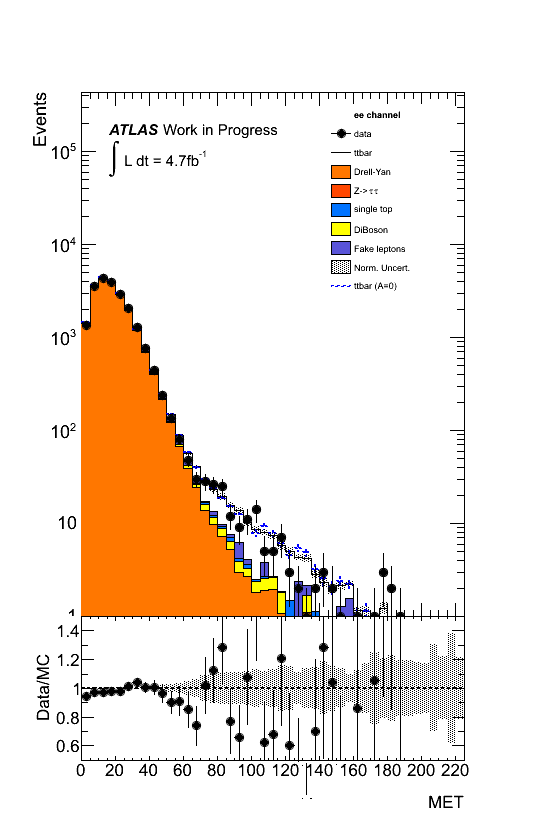
\includegraphics[width=50mm]{f/ee_control_met_central_double}
%     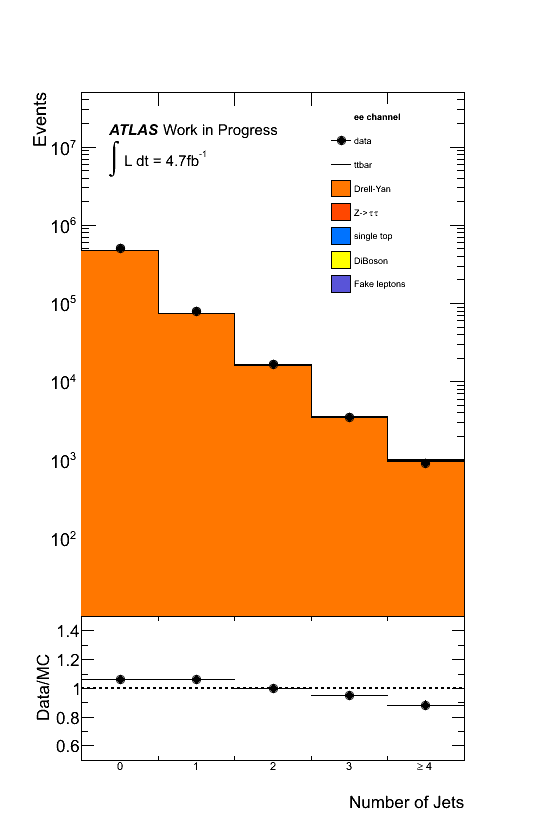
\includegraphics[width=50mm]{f/ee_control_njet_central_double}
%     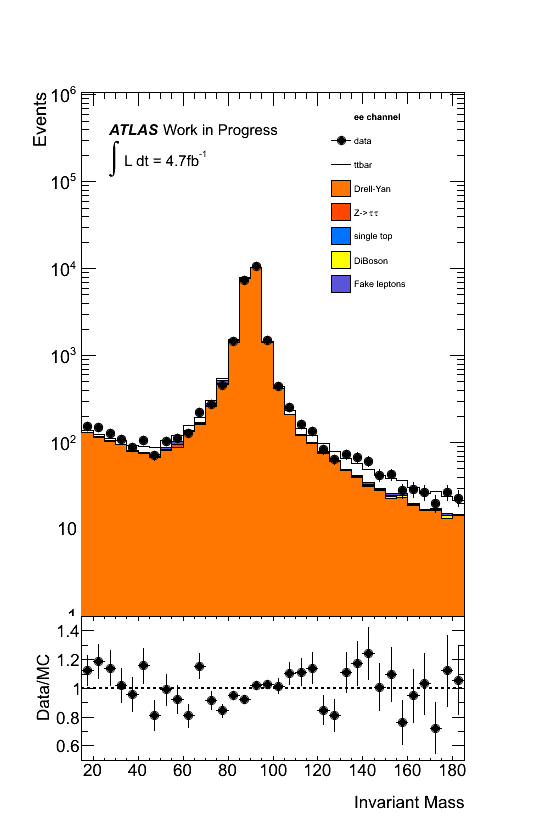
\includegraphics[width=50mm]{f/ee_control_invmass_central_double}
%     \end{center}
%     \caption{Control plots for the \ee\ channel.  \etmiss\ distribution in events with a dilepton mass inside the $Z$-boson mass window and at least two jets (left).  The number of jets in events with a dilepton mass inside the $Z$-boson mass window and \etmiss\ $< 40$~GeV (centre) and the invariant mass of opposite-sign lepton pairs in events with at least two jets and with \etmiss\ $< 40$~GeV (right).}
%     \label{fig:dilep_control_ee}
%     \end{figure}	
    
%\begin{figure}[htbp!]
 %    \begin{center}
%     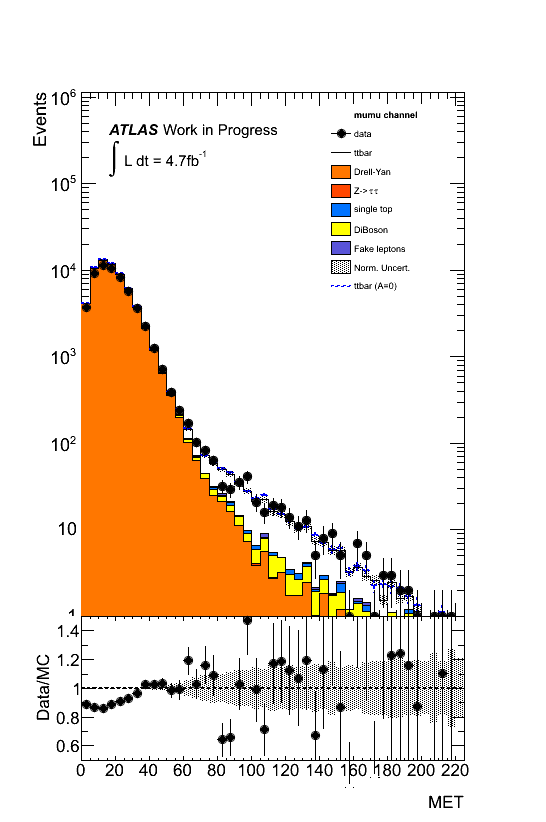
\includegraphics[width=50mm]{f/mumu_control_met_central_double}
%     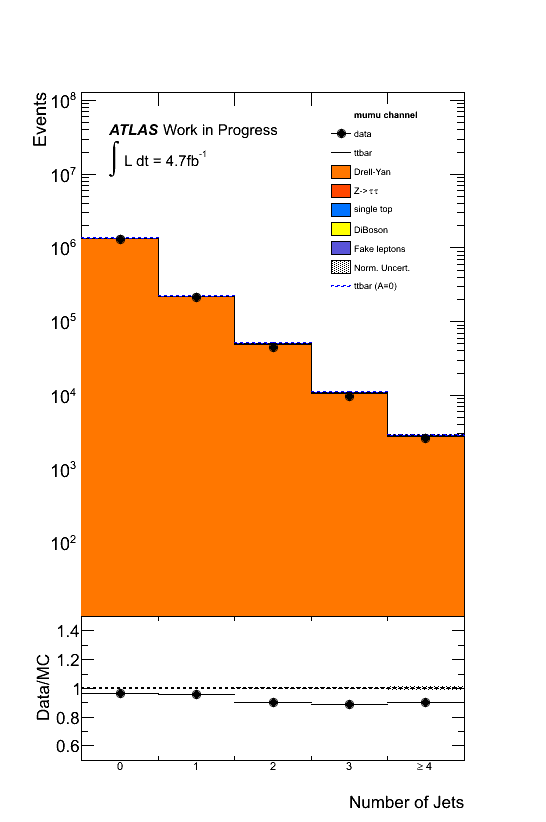
\includegraphics[width=50mm]{f/mumu_control_njet_central_double}
%     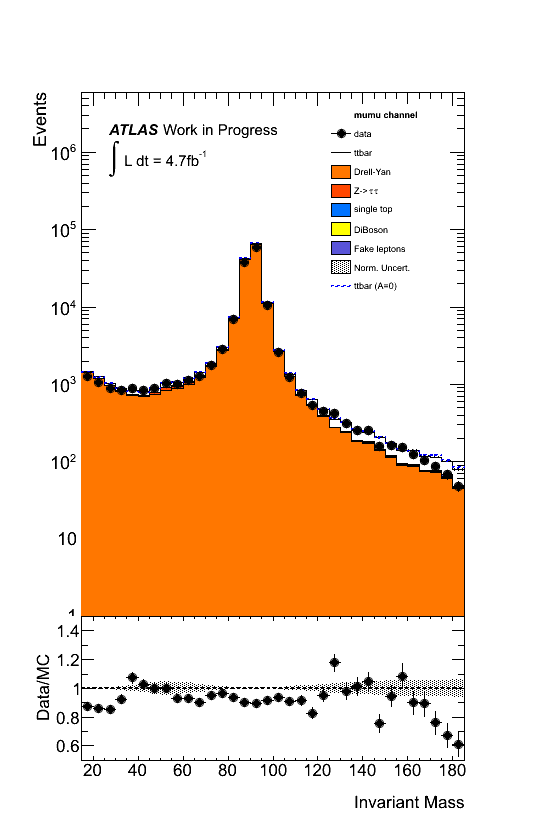
\includegraphics[width=50mm]{f/mumu_control_invmass_central_double}
%     \end{center}
%     \caption{Control plots for the \mumu\ channel.  \etmiss\ distribution in events with a dilepton mass inside the $Z$-boson mass window and at least two jets (left).  The number of jets in events with a dilepton mass inside the $Z$-boson mass window and \etmiss\ $< 40$~GeV (centre) and the invariant mass of opposite-sign lepton pairs in events with at least two jets and with \etmiss\ $< 40$~GeV (right).}
 %    \label{fig:dilep_control_mumu}
 %   \end{figure}

%\begin{figure}[htbp!]
%	\begin{center}
%	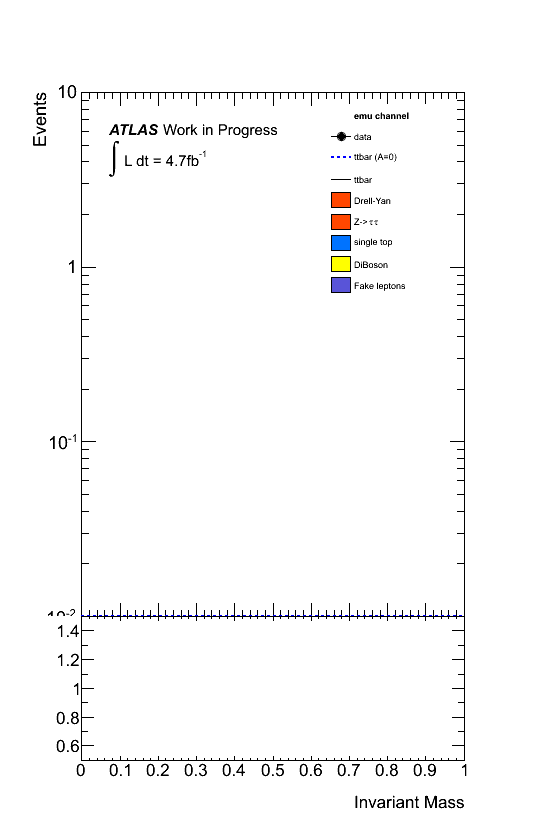
\includegraphics[width=50mm]{f/emu_control_invmass_central_double}
%	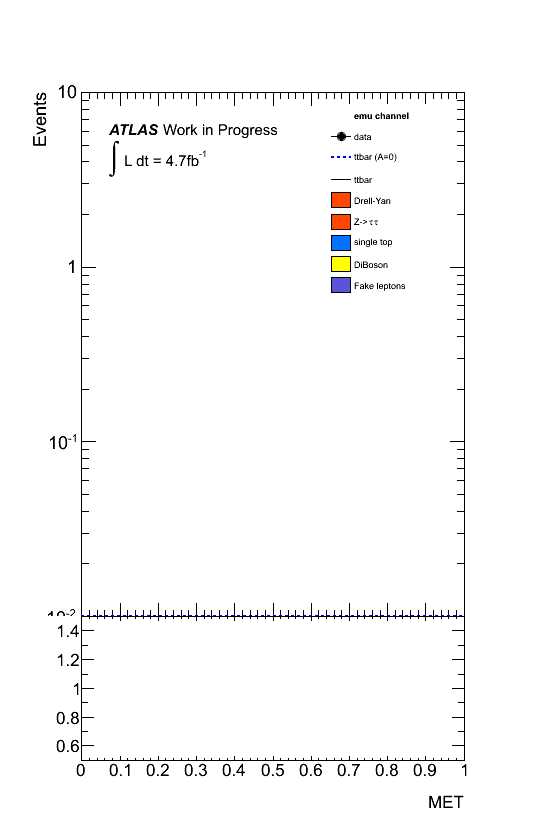
\includegraphics[width=50mm]{f/emu_control_met_central_double}     
%	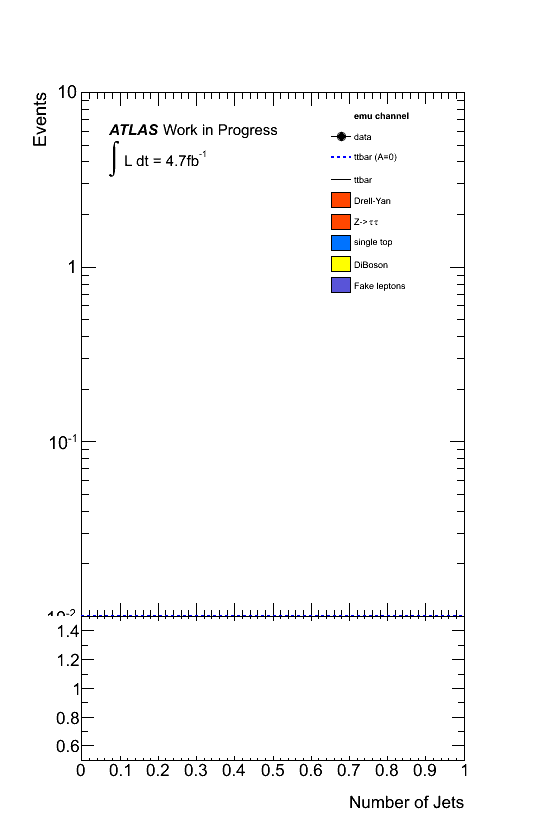
\includegraphics[width=50mm]{f/emu_control_njet_central_double}
%	\end{center}
%	\caption{Control distributions for the \emu\ channel. The invariant mass distribution of the electron and muon (left), the \etmiss\ distribution and the jet multiplicity distribution}
%	\label{fig:dilep_control_emu}
%\end{figure}

\begin{figure}[htbp!]
     \begin{center}
     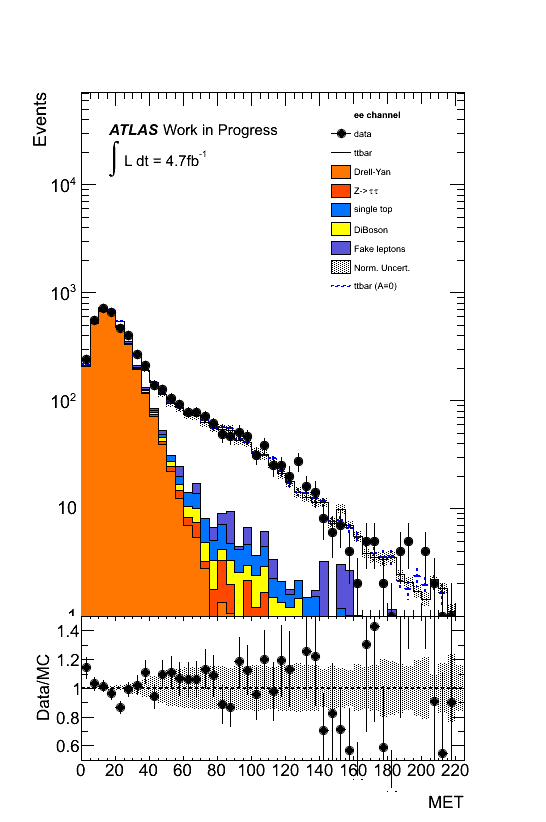
\includegraphics[width=50mm]{f/ee_control_sig_met_central_double}
     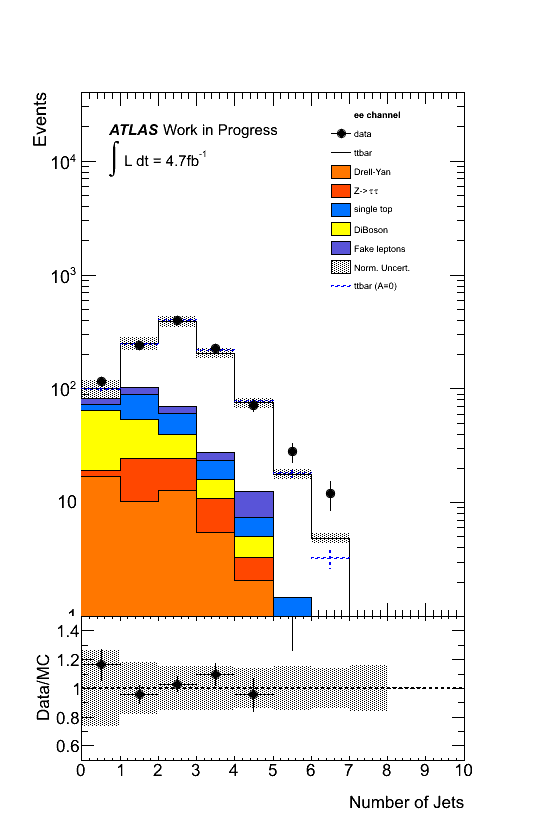
\includegraphics[width=50mm]{f/ee_control_sig_njet_central_double}
     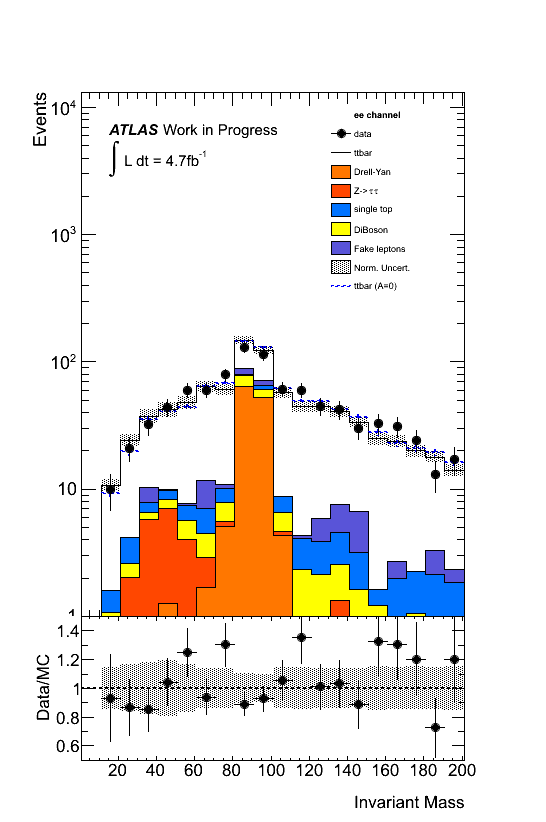
\includegraphics[width=50mm]{f/ee_inv_mass_central_double}
     \end{center}
     \caption{Simulation compared to data in the signal region for the \ee\ channel. The distributions for \etmiss\ , jet multiplicity and invariant mass are shown \emph{left}, \emph{centre} and \emph{right} respectively. In each distribution all selection cuts detailed in section \ref{sec:event_selection} are applied with the exception of the cut applied to the distribution shown.}
     \label{fig:dilep_control_sig_ee}
    \end{figure}

\begin{figure}[htbp!]
     \begin{center}
     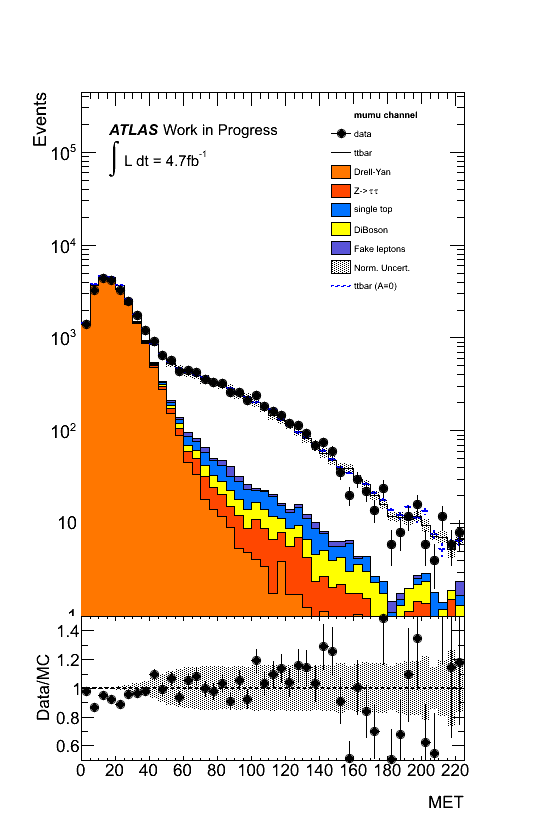
\includegraphics[width=50mm]{f/mumu_control_sig_met_central_double}
     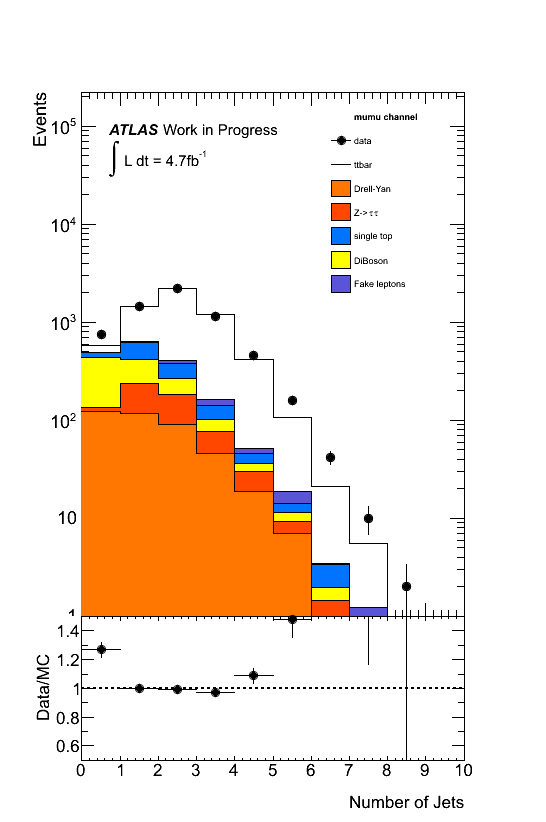
\includegraphics[width=50mm]{f/mumu_control_sig_njet_central_double}
     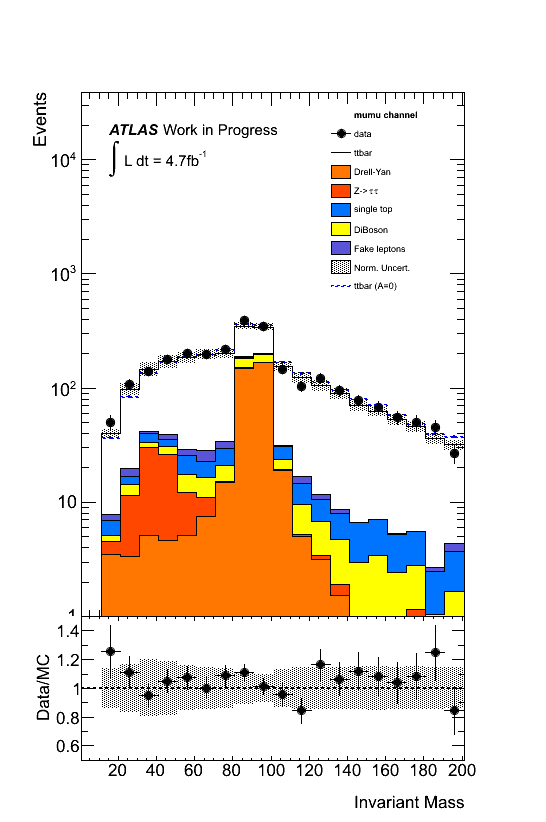
\includegraphics[width=50mm]{f/mumu_inv_mass_central_double}
     \end{center}
     \caption{Simulation compared to data in the signal region for the \mumu\ channel. The distributions for \etmiss\ , jet multiplicity and invariant mass are shown \emph{left}, \emph{centre} and \emph{right} respectively. In each distribution all selection cuts detailed in section \ref{sec:event_selection} are applied with the exception of the cut applied to the distribution shown.}
     \label{fig:dilep_control_sig_mumu}
    \end{figure}

\begin{figure}[htbp!]
     \begin{center}
     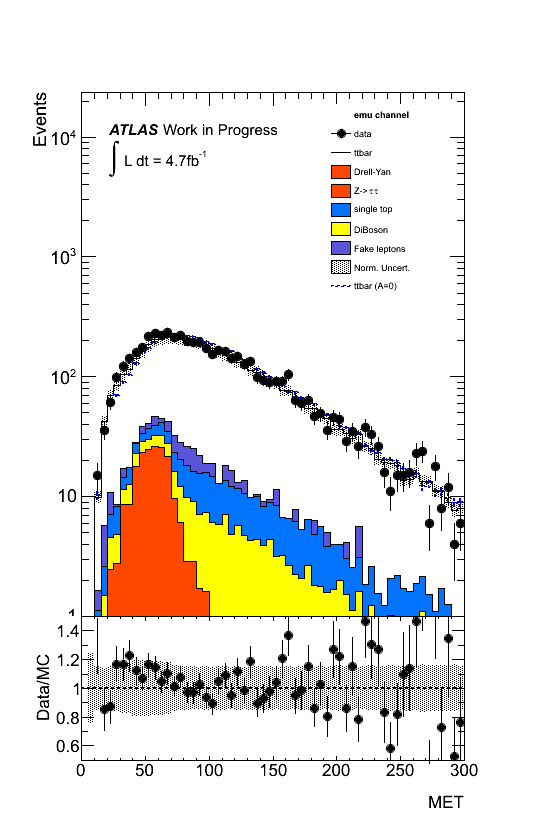
\includegraphics[width=50mm]{f/emu_control_sig_met_central_double}
     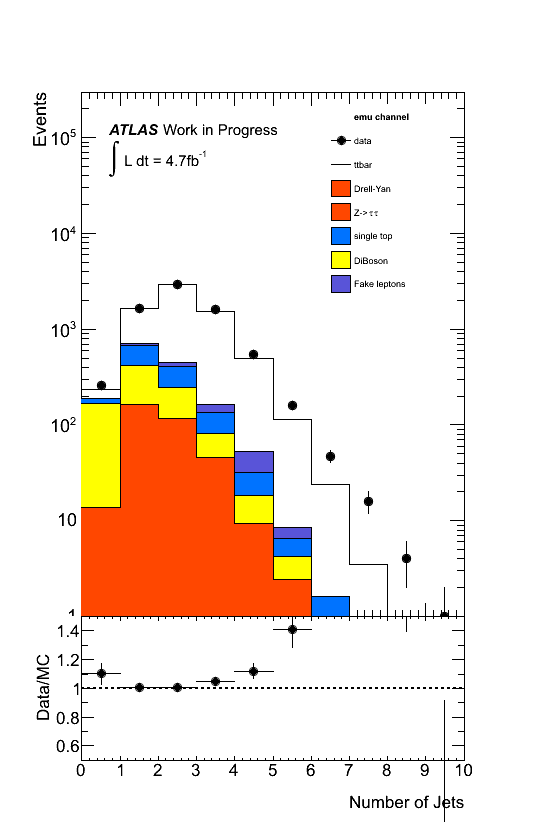
\includegraphics[width=50mm]{f/emu_control_sig_njet_central_double}
     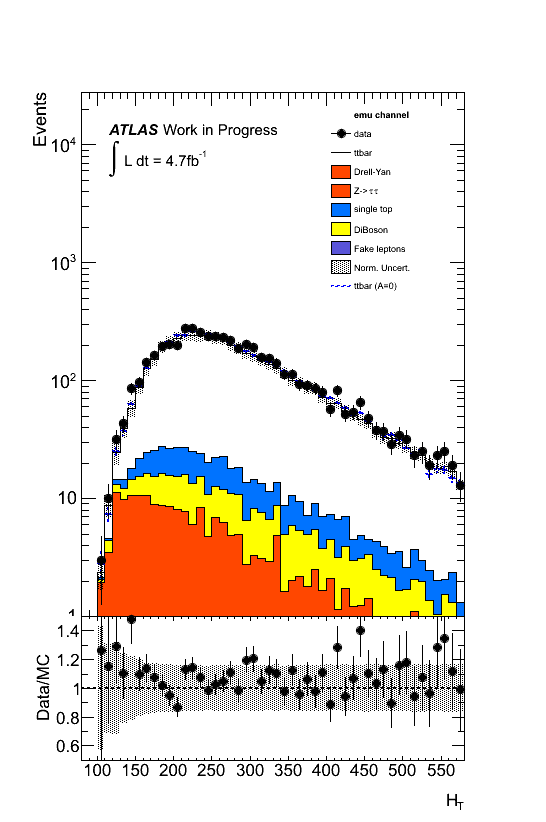
\includegraphics[width=50mm]{f/emu_control_sig_ht_central_double}
     \end{center}
     \caption{Simulation compared to data in the signal region for the \emu\ channel. The distributions for \etmiss\ , jet multiplicity and $H_T$ are shown \emph{left}, \emph{centre} and \emph{right} respectively. In each distribution all selection cuts detailed in section \ref{sec:event_selection} are applied with the exception of the cut applied to the distribution shown.}
     \label{fig:dilep_control_sig_emu}
    \end{figure}

\begin{figure}[htbp!]
     \begin{center}
     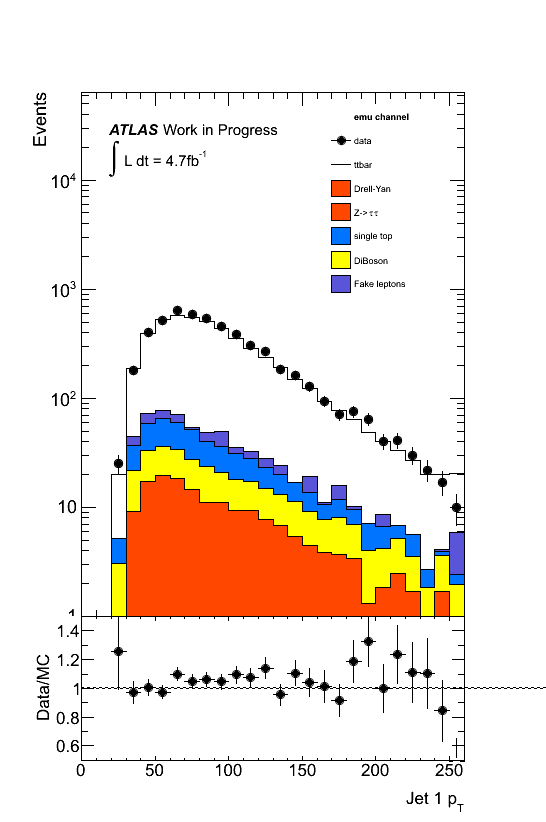
\includegraphics[width=50mm]{f/emu_jet1_pt_central_double}
     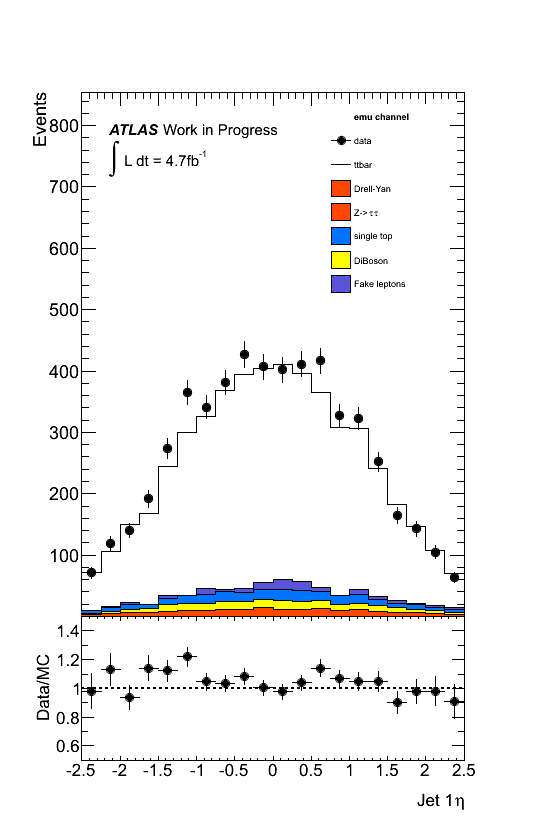
\includegraphics[width=50mm]{f/emu_jet1_eta_central_double}
     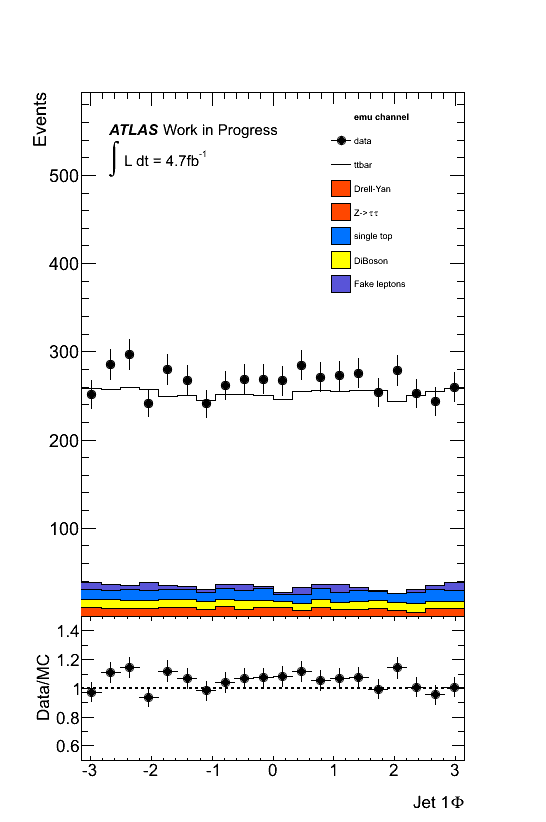
\includegraphics[width=50mm]{f/emu_jet1_phi_central_double}
     \end{center}
     \caption{Distribution of the leading jet \pt\ ,$\eta$, and $\phi$ distributions in the \emu\ channel.}
     \label{fig:dilep_jet1_emu}
    \end{figure}

\begin{figure}[htbp!]
     \begin{center}
     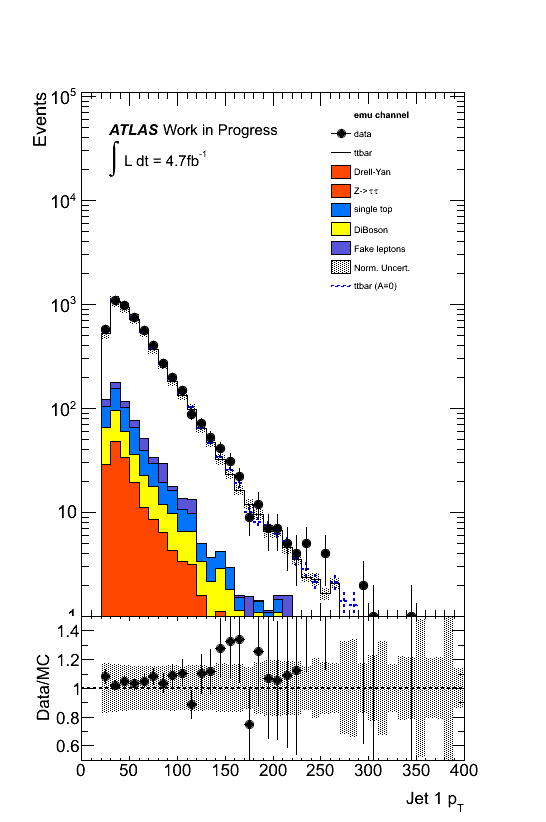
\includegraphics[width=50mm]{f/emu_jet2_pt_central_double}
     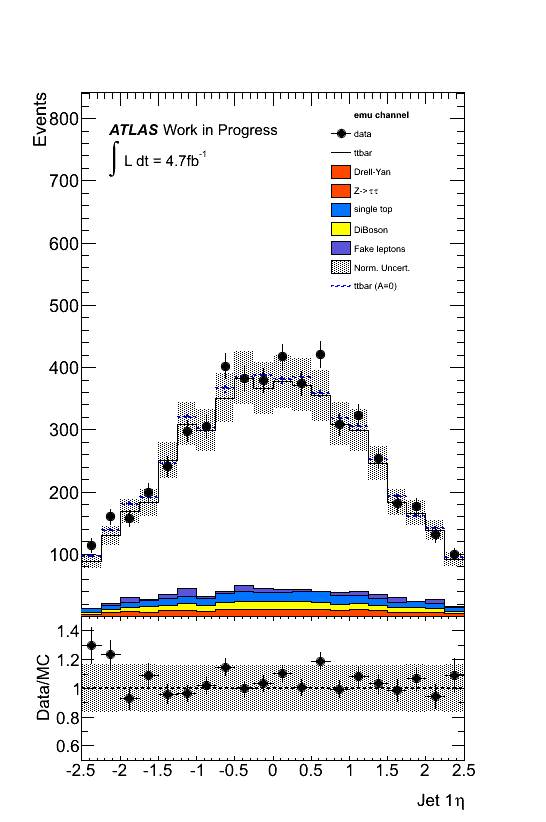
\includegraphics[width=50mm]{f/emu_jet2_eta_central_double}
     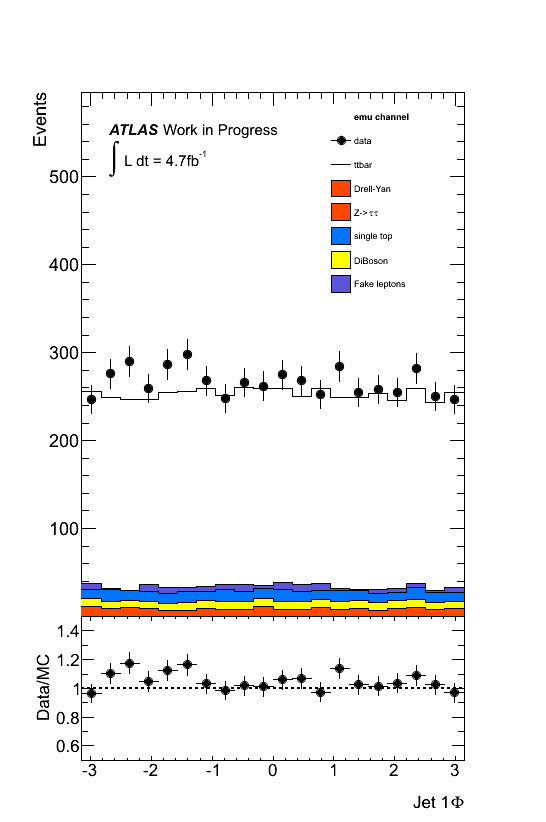
\includegraphics[width=50mm]{f/emu_jet2_phi_central_double}
     \end{center}
     \caption{Distribution of the leading jet \pt\ ,$\eta$, and $\phi$ distributions in the \emu\ channel.}
     \label{fig:dilep_jet2_emu}
    \end{figure}

\begin{figure}[htbp!]
     \begin{center}
     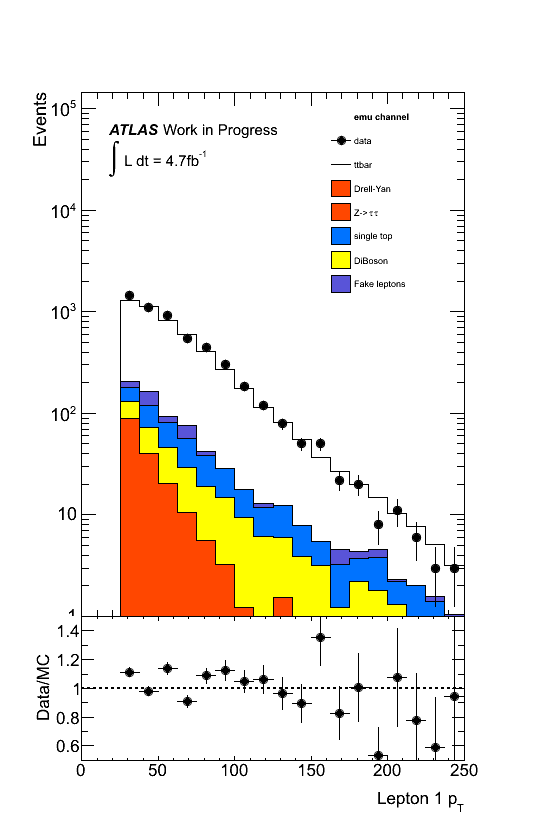
\includegraphics[width=50mm]{f/emu_lep1_pt_central_double}
     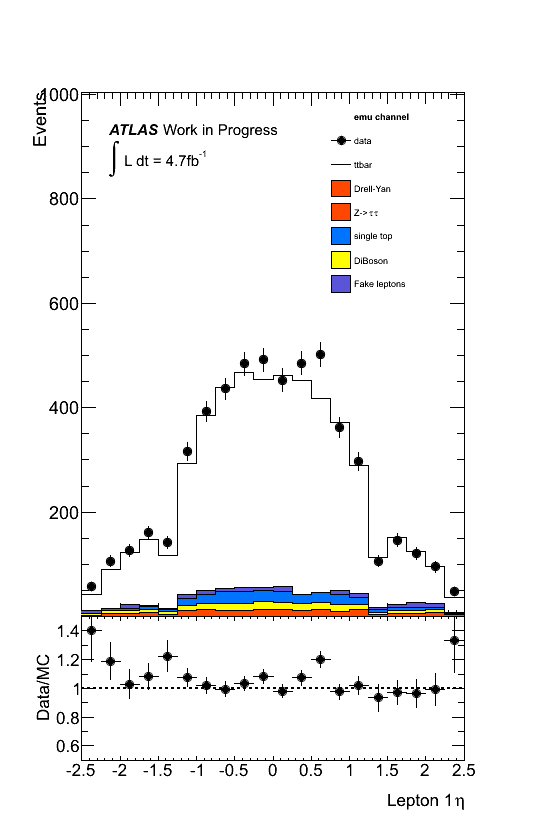
\includegraphics[width=50mm]{f/emu_lep1_eta_central_double}
     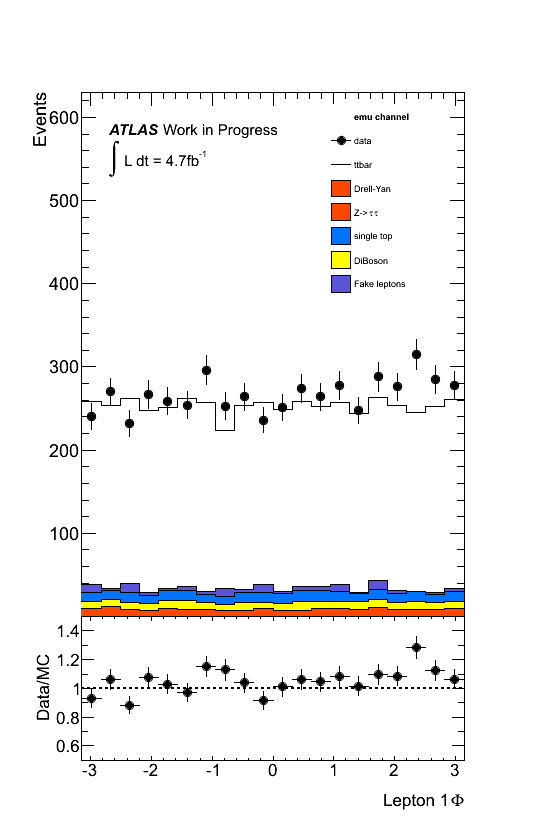
\includegraphics[width=50mm]{f/emu_lep1_phi_central_double}
     \end{center}
     \caption{Distribution of the electron \pt\ ,$\eta$, and $\phi$ distributions in the \emu\ channel.}
     \label{fig:dilep_lep1_emu}
    \end{figure}

\begin{figure}[htbp!]
     \begin{center}
     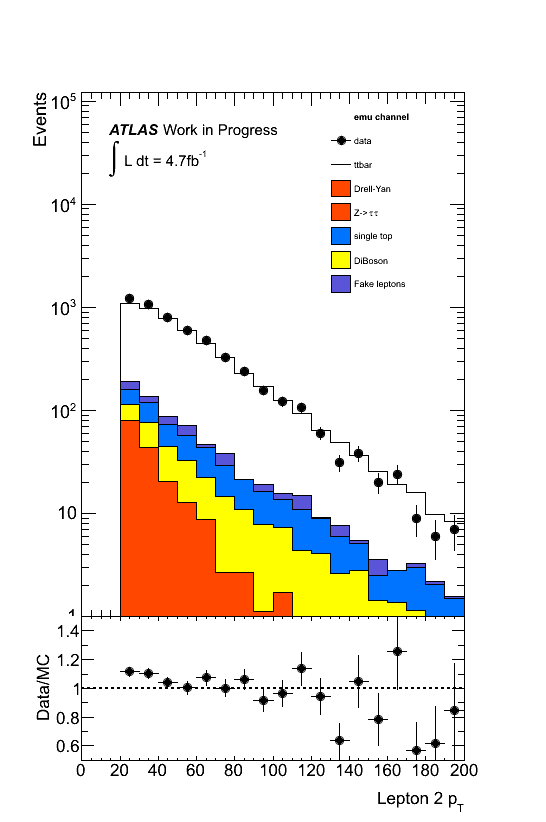
\includegraphics[width=50mm]{f/emu_lep2_pt_central_double}
     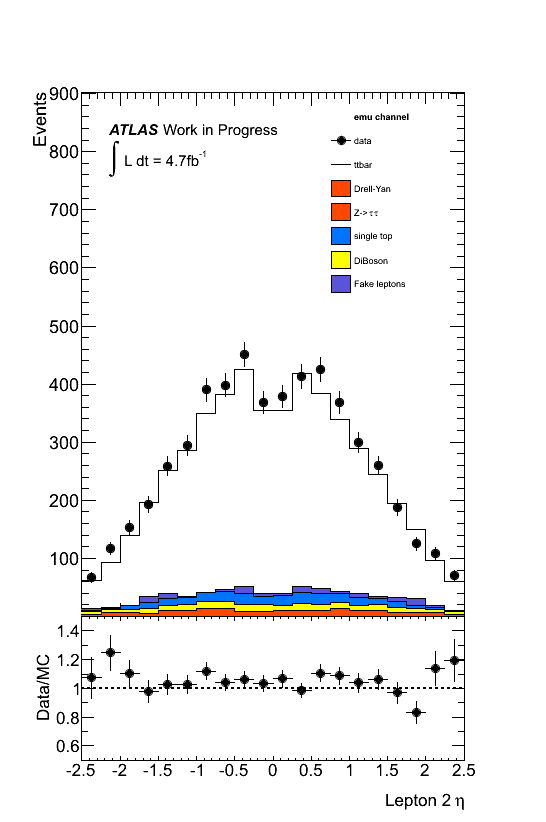
\includegraphics[width=50mm]{f/emu_lep2_eta_central_double}
     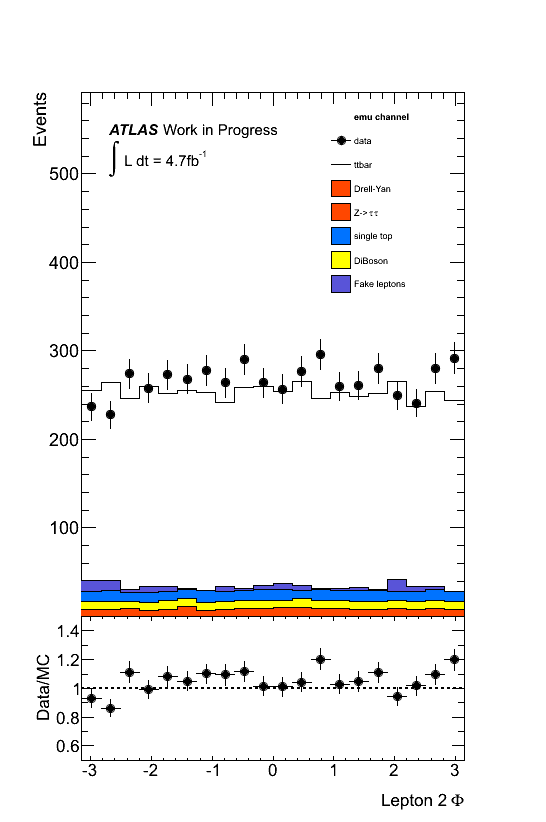
\includegraphics[width=50mm]{f/emu_lep2_phi_central_double}
     \end{center}
     \caption{Distribution of the muon \pt\ ,$\eta$, and $\phi$ distributions in the \emu\ channel.}
     \label{fig:dilep_lep2_emu}
    \end{figure}

\clearpage

\section{Full kinematic reconstruction}
Dilepton \ttbar\ events contain neutrinos. These neutrinos do not interact with the detector so we infer their presence by missing energy in the event. We can only measure this quantity in the transverse direction, \etmiss, and the neutrino's momentum in the z direction must be derived by other means. In the dilepton channel there are two neutrinos but only one measurement for the sum of their transverse momenta, leading to an under-constrained system. Many techniques have been developed to deal with this problem, we describe one of these methods used for this analysis in the following section.

\subsection{Neutrino Weighting}

Neutrino weighting is a reconstruction technique designed to resolve ambiguities inherent to \ttbar\ events with two neutrinos in the final state. It provides the user with reconstructed top quark and neutrino kinematics. %and limited background rejection\footnote{Though not designed to reject background events, typically the reconstruction does not perform well on non-ttbar events and so a small amount of background event rejection is inherent to the method.}. 

One may define a number of kinematic constraints on properties of the \ttbar\ system using known values and assumptions, and use this solve the under-constrained system (full derivation included in Appendix A). The dilepton final state has twelve observable quantities relevant to reconstruction; the reconstructed momenta of the charged leptons and $b$ quark jets. We can also experimentally measure the combined transverse component of the neutrino momenta, however as we shall see this is not used directly to solve the system. Further constraints may be applied by requiring that the two lepton-neutrino pairs combine to give the $W$ boson mass, and that the $W$ boson, $b$-jet pairs combine to give the top mass. Even using all of these quantities, the system is still unconstrained. We can introduce an additional two parameters, the pseudo-rapidities of the un-observed neutrinos, that allows us to fully constrain the system. These pseudo-rapidities ($\eta_1,\eta_2$) cannot be measured experimentally, and so we assign them random values. In other methods the \etmiss\ is used to inform this assumption, however this is not the case for neutrino weighting. A random choice for $\eta_1,\eta_2$ is unlikely to be correct so we must inform this choice as much as possible.
      
      \begin{figure}[h!]
      \begin{center}
     
      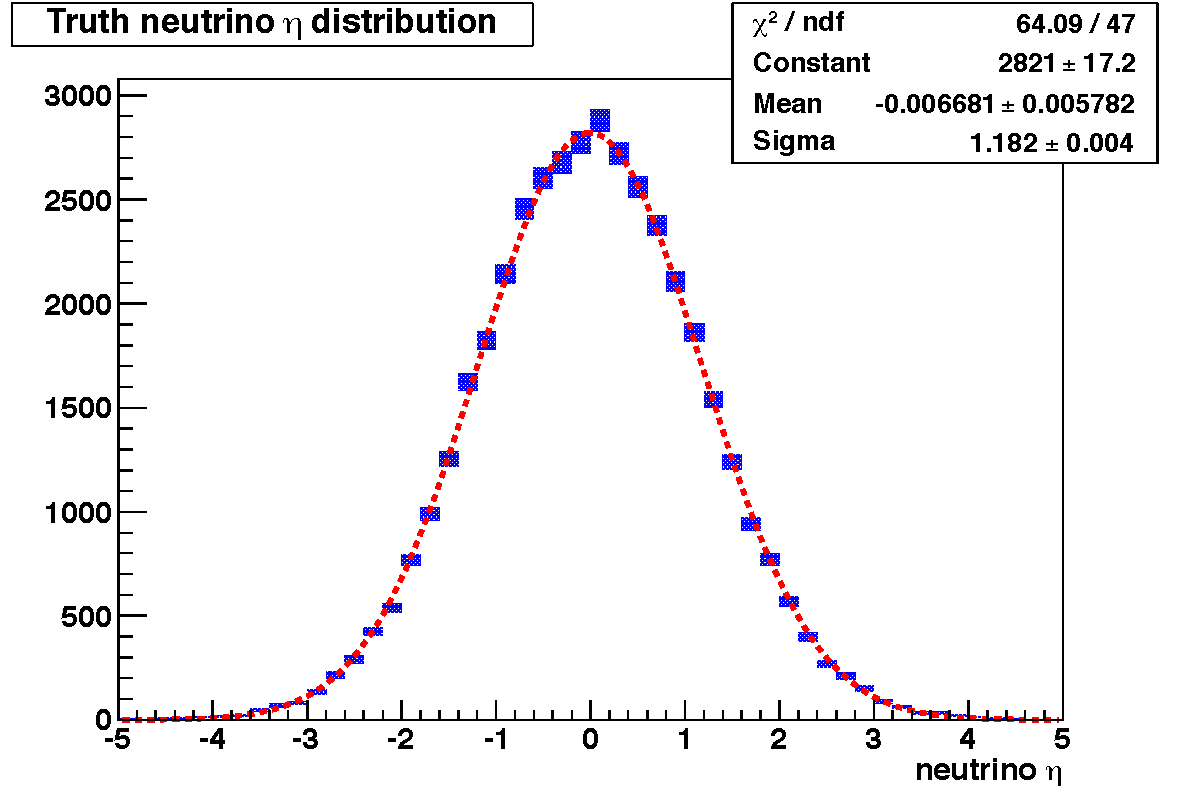
\includegraphics[width=75mm]{f/truth_neutrino_eta}
     
      \caption{Distribution of neutrino pseudo-rapidities in MC@NLO (left) and comparison between neutrino $\eta$ distribution in events with standard model spin correlation and no spin correlation (right)}
      \label{fig:nu_dist}
      \end{center}
      \end{figure}
     
      From Monte-Carlo we can see that the neutrino pseudo-rapidities are well defined as a Gaussian distribution with mean of zero and unit width (Figure \ref{fig:nu_dist}). These distributions are also found to be independent of spin correlation. We perform the reconstruction many times for many different assumptions of neutrino $\eta$. Each event a random $\eta$ is generated for each neutrino using the Gaussian distribution derived from Monte Carlo in the range $-4.0 < \eta < 4.0$. This procedure is repeated 50 times per event and was found to be more effective than previous methods of performing a linear scan of fixed points \cite{Meyer:2007zz}. 

Using the now constrained system the number of solutions per neutrino assumption is 8; two from the ambiguity of the lepton-jet pairing and four (per pairing) from the quadratic terms in the neutrino solution (see Appendix equation XX). The assumption is performed 50 times per neutrino $\eta_i$ assumption, totalling 400 solutions per event.
     
So far we have not used the measured \etmiss\ in the reconstruction, and we have obtained 400 solutions with no information on which is the correct solution, or rather the solution which most accurately reflects the true neutrino four vectors. We can now use the \etmiss\ as a way to weight each solution, based on how well the reconstructed neutrinos agree with the observed \etmiss\ . The function used to calculate this weight is shown in equation \ref{eq:weight}, where $\sigmet$ is the resolution of the $x$ or $y$ component of missing transverse energy~\cite{nuWtmass}. The resolution is the same for the $x$ and $y$ direction and was measured in 7 TeV data and MC~\cite{metres}. The resolution is taken to be $0.66 \sqrt{\Sigma E_T}$ and is shown in figure \ref{fig:met_res}. In a test performed where this resolution was varied by 10\% to account for the differences observed in MC compared to data, no significant effect was noted in the reconstruction.

\begin{figure}[htbp!]
	\begin{center}
	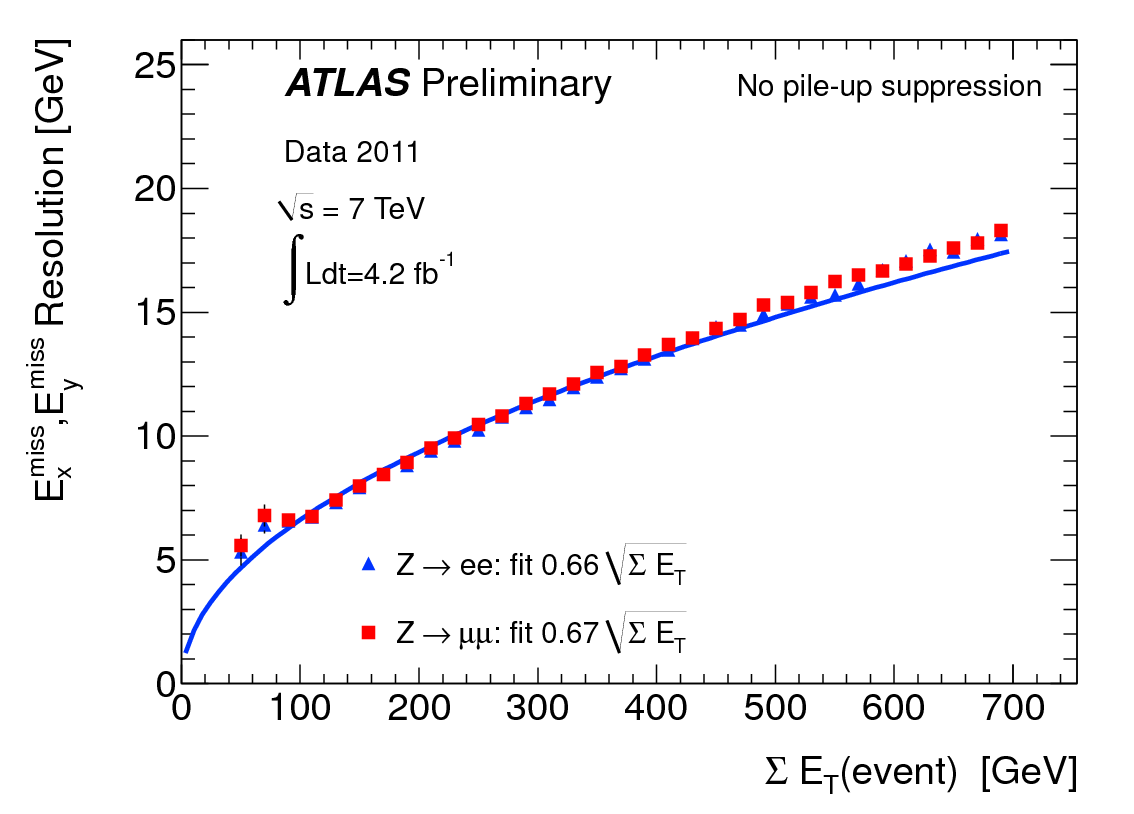
\includegraphics[width=75mm]{f/MET_res_data}
	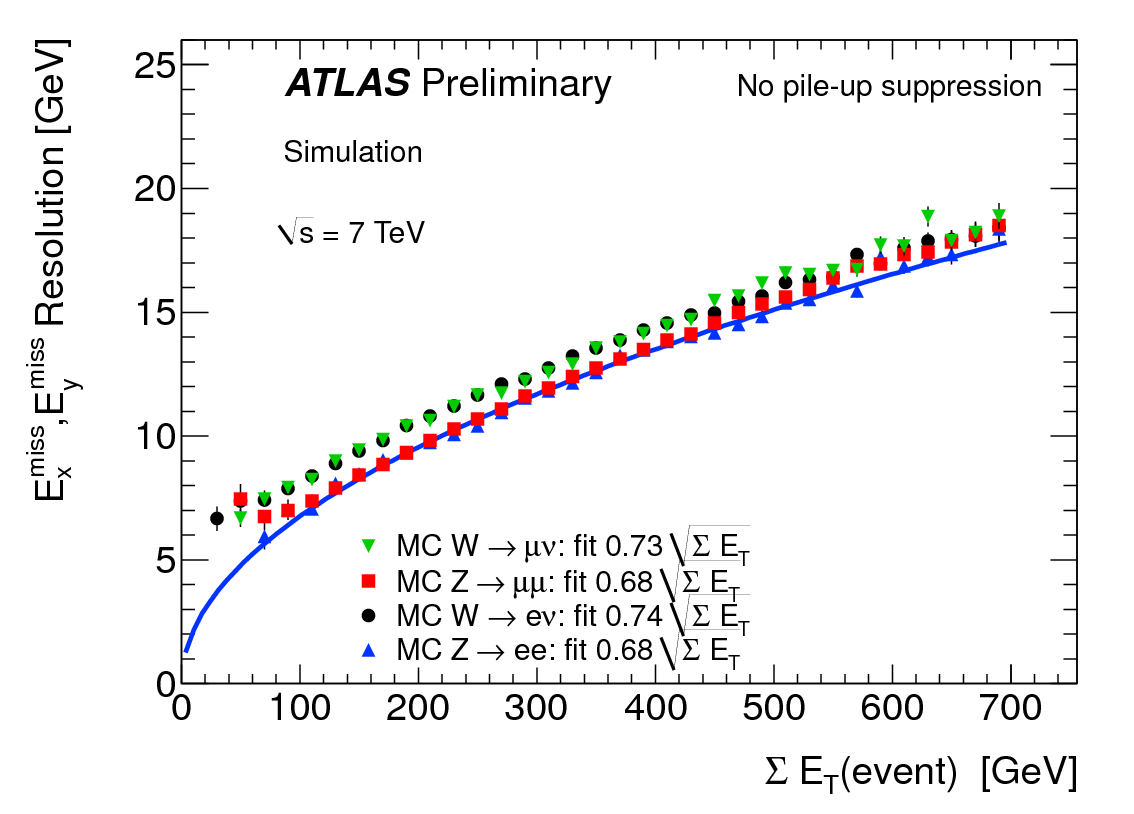
\includegraphics[width=75mm]{f/MET_res_MC}
	\end{center}
	\caption{\etmiss resolution in 2011 data at 7TeV \emph{(left)} and MC \emph{(right)}. }
	\label{fig:met_res}
	\end{figure}

\begin{equation}
    w=\sum_{\eta_{1},\eta_{2}}\sum_{solutions}    
    \exp\left(-\frac{\left(\metx^{calc}-\metx^{obs} \right)^{2}}{2\sigmet} \right)
    \exp\left(-\frac{\left(\mety^{calc}-\mety^{obs} \right)^{2}}{2\sigmet}
    \right)
    \label{eq:weight}
    \end{equation}
     
The final neutrino four momenta may be selected in one of two ways. Either the solution with the highest weight may be chosen, or the weighted sum of all solutions may be taken; the later typically produces better performance. Occasionally an incorrect lepton-jet pairing can give a very high weight whereas in the weighted average this effect is usually mitigated by the combined weights of more accurate solutions.
     
\begin{figure}[htbp!]
	\begin{center}
	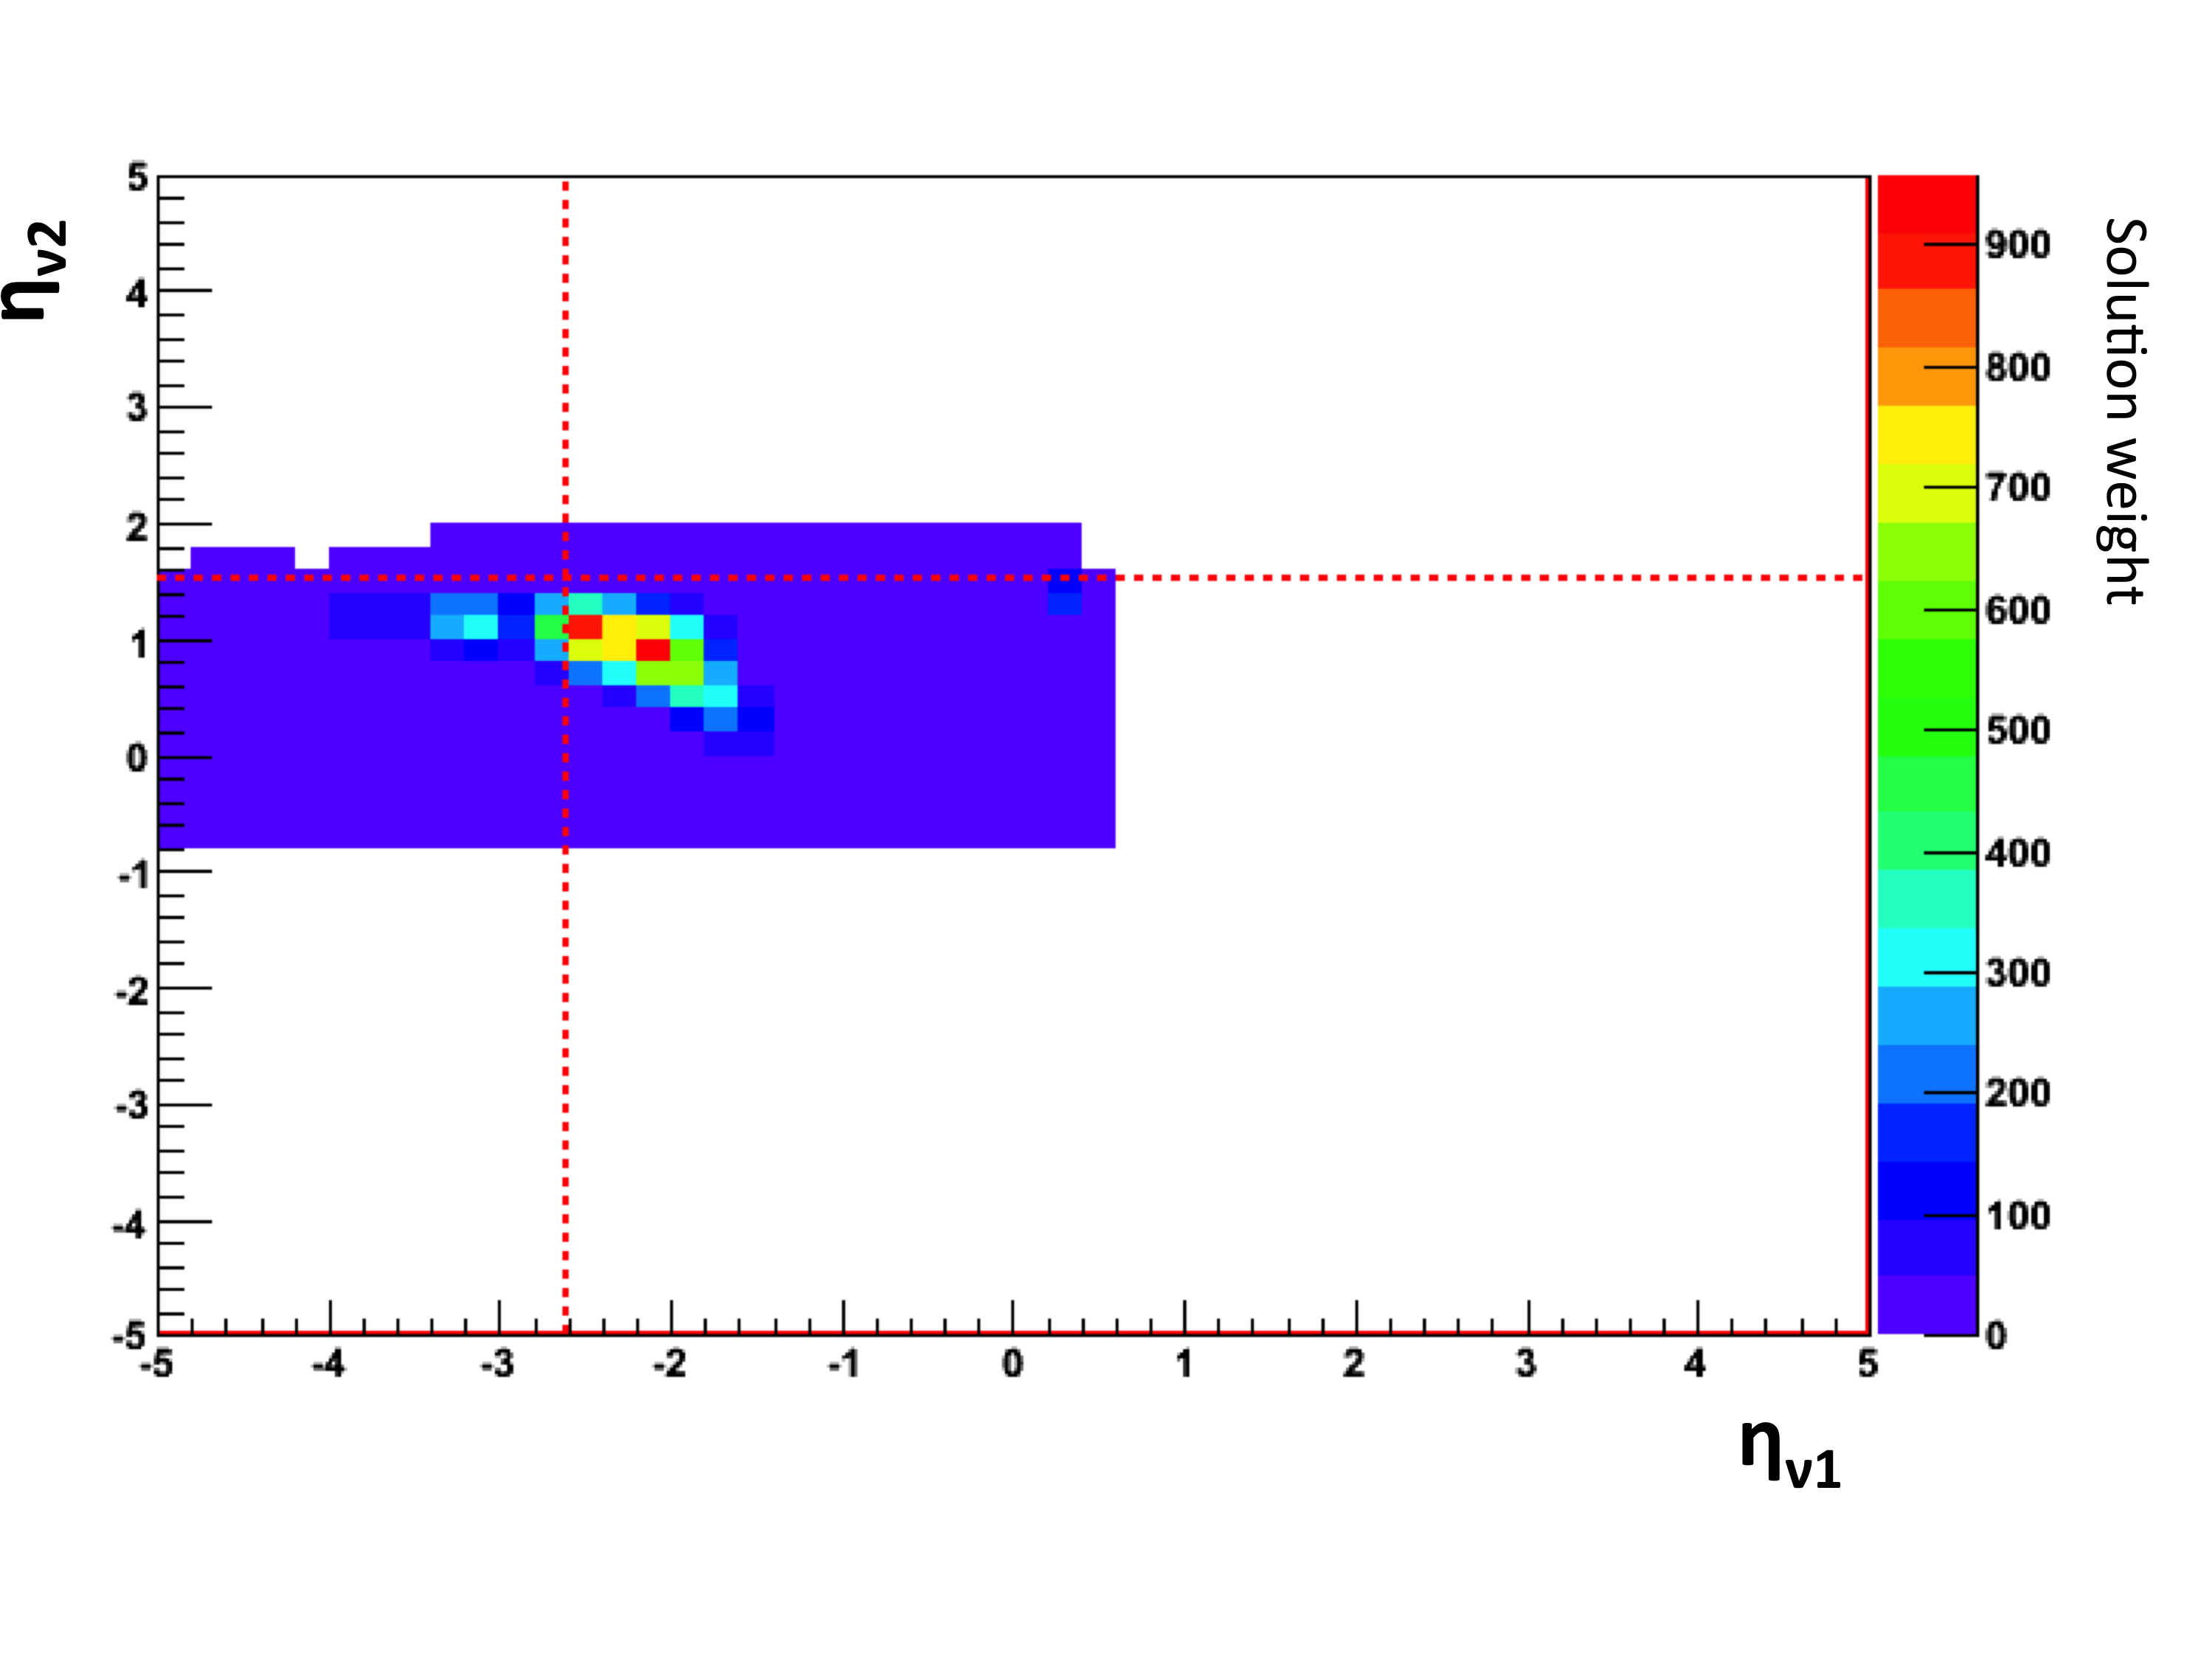
\includegraphics[width=75mm]{f/top_nuweights_1d_2}
	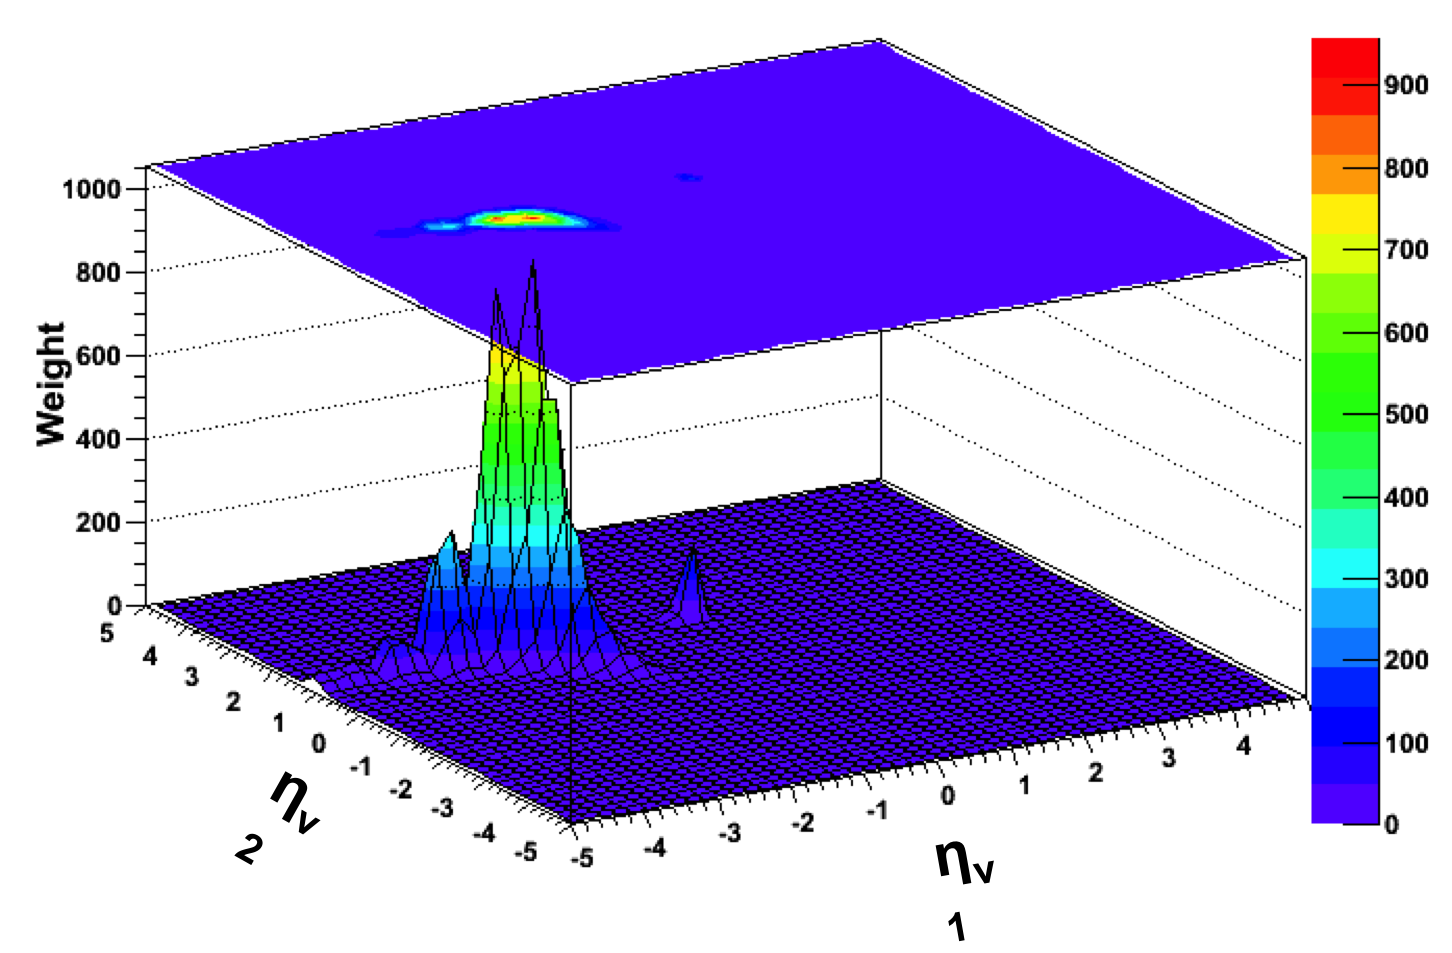
\includegraphics[width=75mm]{f/top_nuweights_2d_2}
	\end{center}
	\caption{Weight distributions for neutrino weighting solutions for a single event. True values for the neutrino $\eta$ are indicated with the red dashed lines.}
	\label{fig:top_nuweights}
\end{figure}

Jet measurements at ATLAS can provide useful information on the underlying parton that seeded them (in this case the b quarks from the top quark decays) however their observed physical quantities, such as energy and direction, are never exactly the same as that of the underlying parton. To account for this, the jet energies are smeared many times for each assumption of $\eta_1\eta_2$ within the measured energy resolution of the jet~\cite{jetres}. The same could be considered for leptons, but at ATLAS the lepton energy resolution is orders of magnitude smaller than the jet energy resolution and hence this is not considered. This was not the case at previous colliders using neutrino weighting (such as D0) and is only applicable to detectors such as ATLAS, where lepton energy resolution is very good.

\subsection{Topology and KLFitter}
Two other reconstruction algorithms are investigated. KLFitter\footnote{There are two implementations of this algorithm, one for dilepton \ttbar\ events and one for semi leptonic \ttbar events. Only the dilepton version is discussed.} is a Kinematic Likelihood Fitter that uses the same numeric solution as neutrino weighting but instead of using a weighting function, uses a likelihood function to qualify solutions. In addition the uncertainty on the b-quark energy is implemented in the likelihood via transfer functions, rather than using energy smearing~\cite{klfitter}.

Topology use the \etmiss\ in the reconstruction directly, using the same constraints as neutrino weighting, leading to only 8 possible solutions per event. The best is chosen using a chi-squared technique~\cite{whelicity}.

Both algorithms utilise information not available in neutrino weighting, the invariant mass of the lepton and b-jet pair. This is useful in removing the lepton-jet pair ambiguity but effectively removes the possibility of considering more than 2 jets in the event for the reconstruction. This will be discussed further in section \ref{sec:reco_comparison}.

\clearpage

\begin{figure}[htbp!]
	\begin{center}
	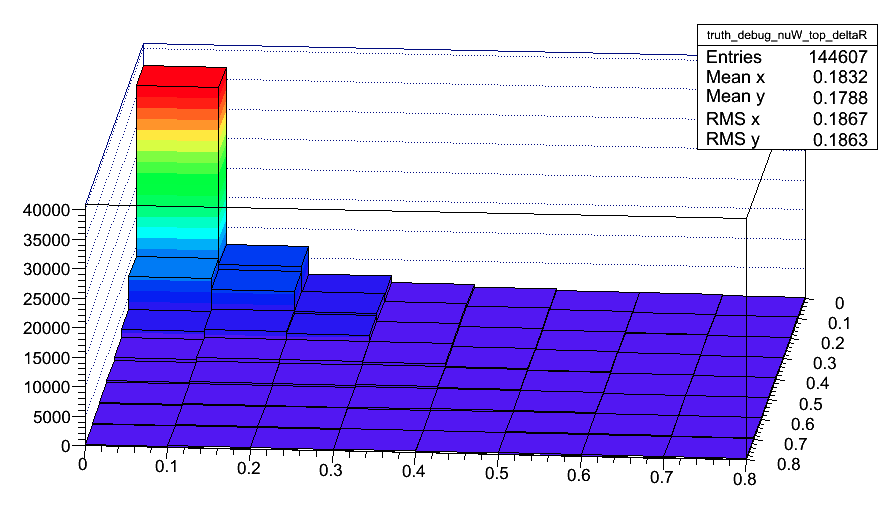
\includegraphics[width=100mm]{f/top_deltaR}
	\end{center}
	\caption{Distance in $\eta - \phi$ space of the reconstructed top to the truth top (x-axis) and the reconstructed anti-top to the true anti-top (y-axis) as a function of absolute number of events.}
	\label{fig:top_dr}
\end{figure}

\subsection{Efficiency}
Three reconstruction algorithms have been discussed in detail (though more exist). In order to compare the advantages and disadvantages of each reconstruction method we define a set of parameters common to each. The parameters are expressed as efficiencies based on the how well the reconstructed particles describe the underlying truth particles in the Monte Carlo. We can use these efficiencies to categorise events where the reconstruction describes the underlying truth information well (matched) and events where the reconstruction did not describe the truth information (unmatched). In this analysis it is the direction of the top quarks that is the most crucial reconstructed quantity and we categorise the events based on how well the top directions are described by the reconstruction. We define the variable $\Delta R (t\bar{t})$ to be the distance in $\eta - \phi$ space of the weighted average \ttbar\ four vectors and the true four vectors in the MC. If this value is less than 0.4 for both the reconstructed top and reconstructed anti-top we say that the event is ``matched" and if not we say that it is ``un-matched". The value of 0.4 is arbitrary since the purpose is not to measure a predictable physical quantity but rather to define a variable with which to compare different reconstruction methods in a consistent way. An example of this variable is shown in figure \ref{fig:top_dr}.


The efficiencies are measured using the nominal \ttbar\ MC@NLO sample and are presented as a fraction of the untagged dilepton selection (total events) and as a fraction of events with at least one solution (solved events). The efficiencies are independent of spin correlation and agree in both MC@NLO samples within the statistical uncertainties. The efficiencies for four cases are shown in table \ref{tab:nu_comparison}. For a selection inclusive of all jets, neutrino weighting had the highest reconstruction efficiency and the highest matched efficiency. KLFitter could not be considered in this selection due to technical limitations of the algorithm and it should be noted that the Topology algorithm was not designed to be used in such a selection. For a selection that include two b-tagged jets (or 1 b-tagged and one high $p_T$ jet) KLFitter has the highest reconstruction efficiency and topology has the highest matched efficiency. The implications of using a b-tagged selection render this unsuitable for this analysis. The reasons for this are described in detail in section \ref{sec:btagged_selection}.
%\vspace{10mm}
\begin{table}[htbp!]
\begin{center}
\footnotesize
%	\begin{tabular}{  c  c  c  c  }
%	\multicolumn{4}{l}{\textbf{ALL JETS}} \\
%	\hline
%	\textbf{Efficiency}       & \textbf{NuW} & \textbf{NuW Mass} & \textbf{Topo} \\
%	\hline
%	\multicolumn{4}{c}{ \textbf{Total events} } \\
%	Reco Eff                  & 96.0 & 96.8 & 82.3 \\
%	$\Delta R(t\bar{t})<0.4$  & 28.5 & 28.5 & 16.1 \\
%	$\Delta R(t\bar{t})<0.2$  & 11.3 & 11.7 &  6.8 \\
%	\hline
%	\multicolumn{4}{c}{ \textbf{Solved events} } \\
%	$\Delta R(t\bar{t})<0.4$  & 29.7 & 29.5 & 19.6 \\
%	$\Delta R(t\bar{t})<0.2$  & 11.8 & 12.1 &  8.3 \\	
%	\hline
 %   \end{tabular}
%    \quad
 %   \begin{tabular}{ c c c c }
	%\multicolumn{4}{l}{\textbf{B-TAGGED}} \\
%	\hline
%	\textbf{Efficiency}       & \textbf{NuW} & \textbf{Topo} & \textbf{KLfitter*} \\
%	\hline
 %   \multicolumn{4}{c}{ \textbf{Total events} }    \\
%	Reco Eff                  & 62.8 & 66.7 & 70.0 \\
%	$\Delta R(t\bar{t})<0.4$  & 18.3 & 26.5 & 22.0 \\
%	$\Delta R(t\bar{t})<0.2$  &  8.9 & 11.2 &      \\
%	\hline
 %   \multicolumn{4}{c}{ \textbf{Solved events} }   \\
%	$\Delta R(t\bar{t})<0.4$  & 29.1 & 39.7 & 31.4 \\
%	$\Delta R(t\bar{t})<0.2$  & 14.1 & 16.8 &      \\	
%	\hline	
%	\end{tabular}
%	\end{center}
%	\caption{Table of Neutrino weighting (NuW) and Topology (Topo) reconstruction efficiency. Two cases are shown, the case for an inclusive selection and for a double b-tagged selection (where events with only one b-tagged jet are included and the second jet is the highest \pt\ non b-tagged jet). The case where the top mass constraint is flucutated in NuW is also shown. \\ \\ \footnotesize{*KLfitter numbers were provided by independent analysers on limited statistics and hence has much larger uncertainties than Topo of NuW}}

	\begin{tabular}{  c  c  c  }
	\multicolumn{3}{l}{\textbf{ALL JETS}} \\
	\hline
	\textbf{Efficiency}       & \textbf{NuW} & \textbf{Topo} \\
	\hline
	\multicolumn{3}{c}{ \textbf{Total events} } \\
	Reco Eff                  & 96.0 & 82.3 \\
	$\Delta R(t\bar{t})<0.4$  & 28.5 & 16.1 \\
	$\Delta R(t\bar{t})<0.2$  & 11.3 &  6.8 \\
	\hline
	\multicolumn{3}{c}{ \textbf{Solved events} } \\
	$\Delta R(t\bar{t})<0.4$  & 29.7 & 19.6 \\
	$\Delta R(t\bar{t})<0.2$  & 11.8 &  8.3 \\	
	\hline
   \end{tabular}
    \quad
\quad	
\quad
    \begin{tabular}{ c c c c }
	\multicolumn{4}{l}{\textbf{B-TAGGED}} \\
	\hline
	\textbf{Efficiency}       & \textbf{NuW} & \textbf{Topo} & \textbf{KLfitter*} \\
	\hline
    \multicolumn{4}{c}{ \textbf{Total events} }    \\
	Reco Eff                  & 62.8 & 66.7 & 70.0 \\
	$\Delta R(t\bar{t})<0.4$  & 18.3 & 26.5 & 22.0 \\
	$\Delta R(t\bar{t})<0.2$  &  8.9 & 11.2 &      \\
	\hline
    \multicolumn{4}{c}{ \textbf{Solved events} }   \\
	$\Delta R(t\bar{t})<0.4$  & 29.1 & 39.7 & 31.4 \\
	$\Delta R(t\bar{t})<0.2$  & 14.1 & 16.8 &      \\	
	\hline	
	\end{tabular}
	\end{center}
	\caption{Table of Neutrino weighting (NuW) and Topology (Topo) reconstruction efficiencies in two selections. B-TAGGED is defined as the two highest $p_T$ b-tagged jets or, in the case of only one b-tagged jet in the event, the highest $p_T$ non b-tagged jet is used. \\ \\ \footnotesize{*KLFitter numbers were provided by independent analysers on limited statistics and hence has much larger uncertainties than Topo of NuW}}
\label{tab:nueff}
\end{table}



%\begin{table*}[!h]
%\begin{center}
%\scriptsize
%  \begin{tabular}{ c | c  c | c  c | c  c}
%    \hline
%    \textbf{Efficiency} & \textbf{ee (tot)} & \textbf{ee (rel)} & \textbf{$\mu\mu$ (tot)} & \textbf{$\mu\mu$ (rel)} & \textbf{e$\mu$ (tot)} & \textbf{e$\mu$ (rel)} \\
%    \hline
%    Reconstructed events               & 96.0 &      & ---- &      & ---- &      \\
%    \hline
%    $\Delta R (t\bar{t}) < 0.4$        & 19.7 & 24.2 & 25.4 & 33.1 & 22.7 & 30.3 \\
%    $\Delta R _(t\bar{t}) < 0.2$       &  7.6 &  9.4 & 10.7 & 13.9 &  9.3 & 12.5 \\
%    \hline
%    $\Delta R (\nu\bar{\nu}) < 0.4 $   &  1.9 &  2.3 &  4.7 &  6.1 &  2.5 &  3.3 \\
%    $\Delta R (\nu\bar{\nu}) < 0.2 $   &  0.0 &  0.0 &  0.0 &  0.0 &  2.5 &  3.3 \\
%    \hline
%    Correct Pair                       &      &      &      &      &      &      \\
%    All top correct                    &  8.3 & 10.2 &  8.7 & 11.4 &  7.4 &  9.9 \\
%    \hline
%    \end{tabular}
%  \end{center}
%	\label{tab:nu_eff}
%  \caption{Table showing the efficiencies of the mean weighted reconstruction in ttbar Monte Carlo.}
%\end{table*}

\subsubsection{Performance on signal Monte Carlo}
The efficiencies for neutrino weighing were measured in both the SM sample and the uncorrelated sample. No difference was observed in the reconstruction efficiencies however an interesting effect was observed in distribution shapes. Events with spin correlation included where no truth matching is achived are indistinguishable from uncorrelated events as shown in figure \ref{fig:matching}. This is a useful feature as unmatched events do not distort the shape of the matched events. If the shape of the unmatched events had been somehow anti-correlated with those that matched the overall sensitivity might have been reduced. The conclusion is that poorly reconstructed events simple act as a flat background in the extraction method (described in section \ref{sec:extraction}) and do not detract from the separation of the two hypotheses templates. This result only applied to neutrino weighting and cannot be assumed for other reconstruction methods.

\begin{figure}[htbp!]
	\begin{center}
	\includegraphics[width=75mm]{f/ee_coscosop_matching}
	\includegraphics[width=75mm]{f/emu_coscosop_matching}
	\includegraphics[width=75mm]{f/mumu_coscosop_matching}
	\end{center}
	\caption{Comparison between the unmatched \ttbar\ events in signal MC to the matched \ttbar\ events. Unmatched event distributions appear more symmetrical similar to distributions in the uncorrelated MC.}
	\label{fig:matching}
	\end{figure}


\subsubsection{Performance on background Monte Carlo}
In principle, the weight distribution may contain information useful for background suppression. Background events should be harder to reconstruct and provide on average lower weights. If one were to cut on the weight distribution magnitude, it may be possible to suppress background. This analysis was formulated to be as inclusive as possible, and relies on good understanding of the background shapes rather than attempting to fully remove them and so this possible feature was not used. A further study could include an investigation into this possibility and would be particularly useful for analyses that wished to perform multi-dimensional unfolding of reconstructed distributions where additional background suppression would be desirable. 

\subsubsection{Comparison with other methods}
\label{sec:reco_comparison}
The Neutrino Weighting algorithm was compared to two other reconstruction algorithms; KLFitter$_{dilepton}$ and Topology. Neither algorithm is capable of considering an inclusive jet selection and so the constraint is made that only two jets are selected with at least one b-tag. In cases where there are more than two b-tags, the two with the highest \pt\ are chosen. A selection where the two jets with the highest b-tag weight were used was also investigated, however the conclusions in both cases remains the same.

Both algorithms give higher efficiency of matched \ttbar\ events than neutrino weighting. This is due to an extra component available in both. The lepton-jet invariant mass distribution is sensitive to correct or incorrect lepton-jet pairings, as shown in figure \ref{fig:lep_jet_mass}. In the simple case of two jets, the difference between the invariant masses tends to be negative for correct pairings. It is not possible to perform this cut in neutrino weighting due to the inclusive jet selection. 

\begin{figure}[htbp!]
     \begin{center}
     \includegraphics[width=100mm]{f/InvariantMassLepBjet}
     \end{center}
     \caption{Invariant mass distribution for lepton-jet pairings. The correct pairing is shown in red, the incorrect pairing is shown in blue. The data is shown in black.}
     \label{fig:lep_jet_mass}
    \end{figure}
%InvariantMassLepBjet


Due to the loss of statistics in KLFitter and Topology by only considering two jets, neutrino weighting still reconstructs an absolute number of events similar to that of KLFitter and Topology and no clear advantage exists between the methods. In principle all three could include the positive aspects of the others, resulting in one inclusive algorithms with higher performance than any algorithm alone. To date no such algorithm exists.


\subsubsection{Application of b-tagging}
\label{sec:btagged_selection}
The requirement of one or more b-tagged jets in an event does much to aid in background rejection but at the cost of statistics ($\sim35\%$ for two b-tags). In events at the LHC it is common for there to be higher jet multiplicities than would arise from the LO hard scatter alone. This may be due to initial and final state gluon radiation (in the case of higher order corrections) or poorly suppressed pile up. In \ttbar\ events, one might expect that the addition of b-tagging would aid in final state reconstruction, by identifying the jets from the top decay and rejecting other contributions. The reconstruction efficiency would be expected to increase for the same reason, with less jets to confuse the reconstruction it should perform better. In reality this is not the case as can be seen in table \ref{tab:nu_comparison}. The fraction of solved events that matched the truth \ttbar\ four momenta within a $\Delta R$ cone of 0.4 does not increase with the addition of b-tags. The reason for this counter intuitive result can be understood with an example.

\begin{figure}[htbp!]
     \begin{center}
     \includegraphics[width=75mm]{f/top_gluon_emission}
     \end{center}
     \caption{Cartoon showing a dileptonic \ttbar\ event where an additional jet from gluon final state radiation has been incorrectly identified as one of the b-jets coming from the top decay.}
     \label{fig:dilepton_cartoon}
    \end{figure}

\begin{figure}[htbp!]
     \begin{center}
     \includegraphics[width=75mm]{f/top_gluon_emission_2}
     \end{center}
     \caption{Cartoon showing a dileptonic \ttbar\ event where both b-jets were identified as coming from the top decay.}
     \label{fig:dilepton_cartoon2}
    \end{figure}

Let us imagine that we have a dileptonic \ttbar\ event in our signal MC, with at least one additional jet (3+ total). Two jets are tagged as having b-flavour and a cartoon of this event can be seen in figure \ref{fig:dilepton_cartoon}. We naturally select the two b-tagged jets and only use these in the neutrino weighting algorithm, the non b-tagged jets are not considered. The reconstruction performs poorly, and when we examine the true \ttbar\ 4-vectors we find that we have not reconstructed the system correctly. Why did this happen? One of the b-tagged jets did not come from the hard scatter, and as a result of only allowing the neutrino weighting algorithm to consider these jets it could not find the correct solution; each solution it did provide (if any) had low weights. Now let us imagine that we considered all possible combinations of jets. The two b-tagged jets still give us solutions with low weight, but now when we consider the non b-tagged jet and look at all possible combinations of jets we obtain solutions with very high weight, peaking around the true values of neutrino pseudo-rapidity such as in figure \ref{top_nuweights}. Clearly we have now included the correct jet pair. When we take the average solution of all jet pairings we guarantee that we will at least examine the correct pairing, and will not be restrained by effects such as miss-tagging.

We must also consider the situation where both b-tagged jets did come from the \ttbar\ and the additional jets are not considered in the reconstruction. In this case we have removed the chance of these incorrect jets contributing fake solutions with high weights, and therefore our reconstruction efficiency would increase.

In reality both situations occur and interfere with each other, resulting in no overall improvement in the reconstruction efficiency with the addiiton of b-tagging, demonstrated in table \ref{tab:nueff}.

By drawing this conclusion we have made several assumptions:

\begin{enumerate}
\item The weights provided by a correct jet pairing are much higher than the weights from an incorrect pairing, and by taking an average we do not suffer from dilutions due to considering many small weighted events. This is illustrated in figure \ref{fig:top_nuweights}.
\item There are a significant proportion of signal events where the two highest \pt\ b-tagged jets do not correspond to the jets arising from the b-quarks. This is shown in table \ref{tab:btag_eff}.
\end{enumerate}

\begin{table}[!h]
	\begin{center}
	\begin{tabular}{ c c c c }
	\hline
	Matching Efficiency & $p_T$ ordered & B-Tag ($p_T$ ordered) & B-Tag (weight ordered) \\
	\hline
	\ee\ channel        & 51.17 \%      & 62.12 \%              & 64.75 \%               \\
	\mumu\ channel      & 52.36 \%      & 63.10 \%              & 65.70 \%               \\
	\emu\ channel       & 54.68 \%      & 64.79 \%              & 67.20 \%               \\
	\hline
	\end{tabular}
	\end{center}
	\caption{Table of reconstructed level particles matched to truth particles. Leptons are required to be matched to a truth lepton within a $\Delta R$ cone of 0.1 and jets are required to be matched to one of the truth b-jets within a $\Delta R$ cone of $0.3$. $p_T$ ordered efficiency is defined as the number of times the two highest $p_T$ jets match the truth b-quarks. B-Tag ($p_T$ ordered) is defined as the number of times the two highest $p_T$ b-tagged jets match the truth b-quarks. B-Tag (weight ordered) is defined as the number of events where two jets with the highest weighted b-tagged jets match the truth b-quarks. In all cases, when only one b-tagged jet exists, the second jet is taken to be the highest $p_T$ non b-tagged jet. }
	\label{tab:btag_eff}
\end{table}

We performed many tests on neutrino weighting with and without b-tagging, summarised in table \ref{tab:nueff}. The relative efficiency of neutrino weighting remains constant, regardless of how many b-tags are applied. We can therefore conclude that overall the addition of b-tagging serves only to suppress background in the selection, and has little effect on the net result of neutrino weighting other than to reduce the number of true signal events that we consider (though event-by-event results can be quite different). The inclusion of extra jets is not detrimental to neutrino weighting as these jets tend to produce results with low weights. This is a unique feature amongst all other \ttbar\ reconstruction algorithms that have been studied. It allows neutrino weighting to consider the full dilepton sample inclusive of all jets; a feature that is simply not available in other methods. 

\subsubsection{Why does neutrino weighting fail?}
The efficiencies described in table \ref{tab:nueff} may seem low, however it is important to understand the difference between inefficiencies caused by limitations of the algorithm and inefficiencies caused by limitations in the event selection. One important factor is that not all hard partons are inside the detector acceptance after reconstruction, but the event may still pass the event selection. If a b-quark is produced at high $\eta$ it is not detected but the event is still likely to pass the selections if there are additional pile-up jets that have not been suppressed. In these cases, we never have the opportunity to correctly use the correct jets in the reconstruction. 

Gluon emission in the final state also produces a situation where we cannot correctly solve the system, our reconstructed four vector for the top quark will have missing momentum and will not match the truth top. 

Finally, our assumption of the range of possible neutrino $\eta$ may not have sufficiently broad and the true neutrino $|\eta|$ may have been greater than 4.0. In MC studies this was shown to occur in less than 0.0001\% of unmatched or failed reconstructions.

All of these features will result in an inefficiency that was not due to shortcomings in the reconstruction algorithm. Some of these effects can be corrected for in the MC with the application of cuts, achieving efficiencies as high as $\sim45\%$ but these require MC truth information and could not be applied on data.

%\subsubsection*{Kinematic Solution}
%\begin{equation*}
 % \begin{aligned}
  %  \\
   % p^{i} & = (E^{i}, \vec{\textbf{p}}^{i}) = (E^{i}, p_{x}^{i}, p_{y}^{i}, p_{z}^{i}) \\
    %p^{i} & = \mbox{contravariant 4-vector of particle of type i}\\
    %m_{i} & = \mbox{mass of particle of type i}\\
    %h = c & = 1 \text{          (working in natual units)} \\
    %\\
    %p_t^i &  = \sqrt{p^{i2}_x + p^{i2}_y} \\
    %\\
  %\end{aligned}
%\end{equation*}
%We may begin with a series of Kinematic constraints:
%\begin{equation}
 % \begin{aligned}
   % \\
   % m_{W} & =(p^{l} + p^{\nu})^2 \\
   % m_{t} & =(p^{l} + p^{\nu} + p^{b})^2 \\
    %\\
  %\end{aligned}
  %\label{nuW:mass_constraint}
%\end{equation}
%We also know from experiment the following quantities:
%\begin{equation*}
 % \begin{aligned}
  %  \\
   % m_{b} = m_{\bar{b}} & = 4.5\GeV \\
   % m_{W} & = 80.4\GeV \\
   %% m_{t} & = 172.5\GeV \\
   % m_{l^+} = m_{l^-} & \approx 0.0\GeV \\
   % m_{\nu} = m_{\bar{\nu}} & \approx 0.0\GeV \\
    %p^{b}, p^{\bar{b}}, p^{l+}, p^{l-} & \mbox{ measured per event}\\
   % \\
    %\end{aligned}
%\end{equation*}
%Although we measure the transverse components of the two neutrino energies via missing energy in the event, this is not used in the kinematic reconstruction but is used as a figure of merit later in the reconstruction procedure. From equation \ref{nuW:mass_constraint} we can expand the equations for $m_{W}$:
%\begin{equation}
  %\begin{aligned}
 %   \\
  %  m_{W}^2 = (E^l + E^{\nu})^2 - (\vec{\textbf{p}}^{l} + \vec{\textbf{p}}^{\nu})^2 & = E^{l^2} + E^{\nu^2} - \vec{\textbf{p}}^{l^2} - \vec{\textbf{p}}^{\nu^2} + 2E^l E^{\nu} - 2\vec{\textbf{p}}^{l} \vec{\textbf{p}}^{\nu} \\
   %  & = 2(E^l E^{\nu} - \vec{\textbf{p}}^{l} \vec{\textbf{p}}^{\nu})\\
    %\\
   % \end{aligned}
%\end{equation}
%We may rearrange this equation for $E^{\nu}$:
%\begin{equation}
 % \\
  %E^{\nu} = |\vec{\textbf{p}}^{\nu}| = \frac{1}{E^l}(\frac{m_{W}^2}{2} + \vec{\textbf{p}}^{l} \vec{\textbf{p}}^{\nu})\\
  %\\
  %\label{nuW:nu_energy_1}%
%\end{equation}
%Similarly we can derive an equivalent equation from the top mass constraint in equation \ref{nuW:mass_constraint}:
%\begin{equation}
 % \begin{aligned}
   % \\
   % m_{t}^2 & = (E^l + E^{\nu} + E^b)^2 - (\vec{\textbf{p}}^{l} + \vec{\textbf{p}}^{\nu} + \vec{\textbf{p}}^{b})^2 \\
    %        & = m_{W}^2 + m_{b}^2 + 2(E^l E^b + E^{\nu} E^{b} - \vec{\textbf{p}}^{l} \vec{\textbf{p}}^{b} - \vec{\textbf{p}}^{\nu} \vec{\textbf{p}}^{b}) \\
    %E^{\nu} & = |\vec{\textbf{p}}^{\nu}| = \frac{m_{t}^2 - m_{W}^2 - m_{b}^2 - 2 p^l p^b}{2 E^b} + \frac{\vec{\textbf{p}}^{\nu} \vec{\textbf{p}}^{b}}{E^b} \\
    %\\
  %\end{aligned}
  %\label{nuW:nu_energy_2}
%\end{equation}
%It is useful to boost into the frame of reference where the neutrinos have no momentum in the direction of the beam, i.e. $p^{\nu}_z = 0$\GeV:
%\begin{equation}
%\begin{aligned}
%\\
%L = 
%\begin{pmatrix}
%\cosh{\eta^{\nu}} & 0 & 0 & -\sinh{\eta^{\nu}} \\
 %       0         & 1 & 0 & 0 \\%
%	0         & 0 & 1 & 0 \\
%-\sinh{\eta^{\nu}}& 0 & 0 & \cosh{\eta^{\nu}}\\
%\end{pmatrix}
%\\
%\end{aligned}
%\end{equation}
%Applying this boost to equation \ref{nuW:nu_energy_1} gives:
%\begin{equation}
%\begin{aligned}
%\\
 % p^{\nu}_T = \frac{m_{W}^2}{2 E^{l^{\prime}}} + \frac{p^l_x p^{\nu}_x}{E^{l^{\prime}}} + \frac{p^l_y p^{\nu}_y}{E^{l^{\prime}}}\\
%\\
%\end{aligned}
%\label{nuW:pt_1}
%^\end{equation}
%where
%\begin{equation}
%\begin{aligned}
%E^{l^{\prime}} = E^l\cosh\eta^{\nu} - p^l_x\sinh{\eta^{\nu}}\\
%\\
%\end{aligned}
%\end{equation}
%Similarly applying this boost to equation \ref{nuW:nu_energy_2} yields:
%\begin{equation}
%\begin{aligned}
%\\
%p^{\nu}_T = \frac{m_{t}^2 - m_W^2 - m_b^2 - 2 p^l p^b}{2 E^{b^{\prime}}} + \frac{p^{\nu}_x p^b_x +  p^{\nu}_y p^b_y}{E^{b^{\prime}}}\\
%\\
%\end{aligned}
%\label{nuW:pt_2}
%\end{equation}
%where
%\begin{equation}
%\begin{aligned}
%E^{b^{\prime}} = E^b\cosh\eta^{\nu} - p^b_x\sinh{\eta^{\nu}}\\
%\\
%\end{aligned}
%\end{equation}
%Equations \ref{nuW:pt_1} and \ref{nuW:pt_2} are equivalent and after solving for $p^{\nu}_x$ one obtains the linear equation:
%\begin{equation}
%\begin{aligned}
%\\
%p^{\nu}_x = ap^{\nu}_y + b \\
%\\
%\end{aligned}
%\label{nuW:px}
%\end{equation}
%where:
%\begin{equation}
%\begin{aligned}
%\\
%a  & = \frac{p^l_y E^{b^{\prime}} - p^b_y E^{l^{\prime}}}{p^b_x E^{l^{\prime}} - p^l_x E^{b^{\prime}}} \\
%\\
%b  & = \frac{E^{l^{\prime}}(m_t^2 - m_W^2 -m_b^2 - 2p^lb^l) - E^{b^{\prime}}m_W^2}{2(p^l_x E^{b^{\prime}} - p^b_x E^{l^{\prime}})}\\
%\\
%\end{aligned}
%\end{equation}
%If we use equation \ref{nuW:px} and the definition of $p_T$ we can rearrange equation \ref{nuW:pt_1} to get:
%\begin{equation}
%\begin{aligned}
%\\
%\sqrt{(a^2 + 1)p^{\nu}_y + 2abp^{\nu}_y + b^2} = \frac{m_W^2}{2E^{l^{\prime}}} + \frac{p^l_x}{E^{l^{\prime}}}(ap^{\nu}_y + b) + \frac{p^l_y}{E^{l^{\prime}}}p^{\nu}_y \\
%\\
%\end{aligned}
%\label{nuW:quad}
%\end{equation}
%If we square equation \ref{nuW:quad} we can obtain a quadratic equation in terms of $p^{\nu}_y$ in the form:
%\begin{equation}
%\begin{aligned}
%\\
%cp^{\nu2}_y + dp^{\nu}_y + f = 0\\
%\\
%\end{aligned}
%\label{nuW:quad2}
%\end{equation}
%with
%\begin{equation}
%\begin{aligned}
%\\
%c & = a^2 + 1 - (\frac{p^l_x}{E^{l^{\prime}}}a + \frac{p^l_y}{E^{l^{\prime}}})^2 \\
%\\
%d & = 2ab - 2(\frac{m_W^2}{2E^{l^{\prime}}} + \frac{p^l_x}{E^{l^{\prime}}}b)(\frac{p^l_x}{E^{l^{\prime}}}a + \frac{p^l_y}{E^{l^{\prime}}})\\
%\\
%f & = b^2 - (\frac{m_W^2}{2E^{l^{\prime}}} + \frac{p^l_x}{E^{l^{\prime}}}b)^2\\
%\\
%\end{aligned}
%\end{equation}
%Equation \ref{nuW:quad2} has two roots. Since we only consider real roots to be physical equation \ref{nuW:quad2} has either 0, 1 or 2 real solutions for $p^{\nu}_y$.
%\begin{equation}
%\begin{aligned}
%\\
%p^{\nu}_y = -\frac{d}{2c}\pm\frac{1}{2c}\sqrt{d^2 - 4cf}\\
%\\
%\end{aligned}
%\end{equation}
%
%Original derivtion taken from (Reference D0 Thesis).
%


\clearpage
\chapter{Extraction of spin correlation}

\section{Likelihood Fit}
\label{sec:extraction}

The amount of spin correlation observed in the data is extracted using a binned maximum likelihood method. Two templates are constructed; one with SM \ttbar\ spin correlations and one with no included \ttbar\ spin correlation. The templates are fit to the data and the degree to which the data fits the SM case is extracted ($f_{SM}$). The cross section of the two \ttbar\ templates taken together is also extracted. 

The likelihood function may be written as:

\begin{equation}
  \begin{aligned}
    =-ln(L) = \mathcal{L} = \displaystyle\sum\limits_{n=0}^{N} Data*\ln\{B + n_{tt}(f_{SM}*S + (1-f_{SM})*NS)\} \\
                  - (B + n_{tt}(f_{SM}*S + (1-f_{SM})*NS) \\
		  - \ln(Data!) \\
  \end{aligned}
\end{equation}

Where $Data$ is the measured number of data events, $S$ is the estimated number of events in the spin sample, $NS$ is the estimated number of events in the uncorrelated sample, $N$ is the number of bins, $n_{tt}$ is the normalisation of the \ttbar\ templates and $B$ is the background estimate. This likelihood function is minimised as function of $f_{SM}$ and the \ttbar\ cross section. The cross section is allowed to vary in order to reduce the influence of normalization uncertainties on the result of $f_{SM}$. For the maximization procedure we use the SIMPLEX and MIGRAD algorithms in the TMinuit package~\cite{James:1975dr}.

The fitting method was validated using a linearity check. The templates were mixed to create pseudo-data sets of simulated spin correlation in the range $f_{SM} = -1 \rightarrow +2$ and the spin correlation extracted. The result is shown in Fig.~\ref{fig:linearity}. No bias is observed in the extraction procedure in the quoted range.

Since each analysis channel is orthogonal, due to the lepton flavour selection, we may multiply the likelihoods to perform a multi channel fit. 

\begin{figure}[h!]
	\begin{center}
	\includegraphics[width=85mm]{f/delta_phi10all_syst_linLinearity}
	\end{center}
	\caption{Linearity check comparing different values of input $f_{SM}$ or \ttbar\ cross section to those extracted by the fit.}
	\label{fig:linearity}
\end{figure}

\section{Systematic Uncertainties}
\label{sec:systematics}

%The use of Monte Carlo simulations in this analysis presents an inherent problem. Though the degree to which these samples accurately reflect the true physics processes that they simulate is impressive, they are not perfect. A systemic disparity occurs between our assumption ( the rates and shapes of the signal and backgrounds distributions ) and the observed data. This is described as a ``systematic'' uncertainty. The effect of these systematic uncertainties, or more simply put the effect of the difference between our simulation and truth, must be quantified. In addition, systematic uncertainties can arrise from effects such as detector modelling, or data driven background estimation techniques and these must also be accounted for. 

The degree to which the systematic uncertainty effects the result is quoted within a 68\% confidence interval (1$\sigma$ deviation) by convention. Ensemble tests are used to estimate the effect of a source of uncertainty. New templates are generated with an estimated 1$\sigma$ shift in the source of uncertainty for both the spin correlated template (spin) and the uncorrelated (no-spin) template.  
Pseudo-data sets are generated by mixing these templates to the observed $f_{SM}$ and Poisson fluctuating their bin content.
The nominal templates are then fitted to the pseudo-data. In addition, the systematic shifted templates are simultaneously fitted to the same pseudo-data and the difference between the two fits are then saved. This procedure is performed 1000 times for each systematic, and the final uncertainty is quoted as the mean of the difference between the two fits.
	The motivation for simultaneously fitting the shifted and the nominal templates to the pseudo-data is to remove statistical fluctuations in the fit. When fitting the shifted templates to the pseudo-data (that has been created from these templates), any deviation from the input spin correlation will be caused by statistical fluctuations in creating the pseudo-data, and will be identical when the nominal templates are fitted to this pseudo-data. By taking the difference between both fits we remove this statistical fluctuation. The step by step procedure for the fitting is summarised below:
 
\begin{enumerate}
	\item Fit the nominal templates $\mathbf{T}_{spin}$, $\mathbf{T}_{nospin}$ to the data $\mathbf{D}$ and obtain $f_{SM}^{nominal}$.
	\item Generate new spin and no spin templates, with a systematic shift \textbf{X} included, $\mathbf{T}^{\mathbf{X}}_{spin}$, $\mathbf{T}^{\mathbf{X}}_{nospin}$.
	\item Construct pseudo data $\mathbf{D^\prime}$ by mixing $\mathbf{T}^{\mathbf{X}}_{spin}$ and $\mathbf{T}^{\mathbf{X}}_{nospin}$ to the observed $f_{SM}^{nominal}$. 
        \item Poisson vary each bin in $\mathbf{D^\prime}$, using the bin content as the mean.
	\item Fit $\mathbf{T}_{spin}$, $\mathbf{T}_{nospin}$ to $\mathbf{D^\prime}$ and obtain $f_{SM}^{\prime}$.
	\item Fit $\mathbf{T}^{\mathbf{X}}_{spin}$, $\mathbf{T}^{\mathbf{X}}_{nospin}$ to $\mathbf{D^\prime}$ and obtain $f_{SM}^{\mathbf{X}}$.
	\item Take the difference $f_{SM}^{\mathbf{X}}$ - $f_{SM}^{\prime}$
	\item Repeat steps 3 $\rightarrow$ 6 1000 times.
	\item Take $<f_{SM}^{\mathbf{X}}$ - $f_{SM}^{\prime}>$ as the systematic uncertainty due to \textbf{X} .
\end{enumerate}

%\begin{figure}[htbp]
%\begin{center}
%\includegraphics[width=100mm]{f/GaussianFigure}
%\end{center}
%\caption{Illustration of systematic estimation procedure. The caussian curve generated by the systemati shifted pseudo experiments is showin in blue, the nominal fit is shown in black}
%\label{fig:syst_gaussian}
%\end{figure}

Each source of systematic uncertainty is assumed to be uncorrelated and for the total systematic uncertainty all of the individual sources are added in quadrature. We give an overview over all sources of systematic uncertainties that we consider and the methods by which they are estimated. For simplicity we categorise systematic uncertainties into two types: 
\begin{itemize}
	\item ``Normalisation uncertainties'': which only effect the rate of a particular background or signal sample.
	\item ``Shape changing systematics'': which effect the shape of the variable of interest, in addition to its normalisation. 
\end{itemize}
Normalisation uncertainties typically have a small effect on the extracted spin correlation as the normalisation of the signal templates is allowed to float in the likelihood fit ( i.e. the floating of the \ttbar\ cross section described in section \ref{sec:extraction}. Shape changing uncertainties are the dominant form of uncertainty in the analysis and can have a marked impact on the spin correlation.

\vspace{5mm}
\noindent
\textbf{Luminosity:}
\begin{itemize} 
     \item For data taken in the 7 TeV LHC running period, the Luminosity uncertainty is taken to be a flat uncertainty of $\pm1.8$~\% on the normalisation of the data, established primarily through Van-De-Meer scans performed during data taking, and comparisons with the CMS detector. The systematic uncertainty is estimated by varying the normalisation of both the signal and background samples simultaneously, up and down by this value.
\end{itemize}

\vspace{5mm}
\noindent
\textbf{Electrons:}
\begin{itemize}
    \item Energy Scale: All electrons are corrected for electron energy scale by default in the Monte Carlo. To estimate the systematic uncertainty this energy scale is shifted by $\pm 1\sigma$ of the uncertainty from the energy scale estimation procedure, in addition to the default scaling. 
    \item Trigger Scale Factor: To estimate the uncertainty on the scale factor associated with trigger modelling, the scale factors are varied by $\pm 1\sigma$~ from the default scale factor.
    \item Energy Resolution: The Monte Carlo is smeared by default to correct for the difference in the modelling of electron energy resolution with the data. Additional smearing is performed to estimate the uncertainty.
\end{itemize}

\vspace{5mm}
\noindent
\textbf{Muons:}
\begin{itemize}
    \item Momentum Shift: There are two possible sources of muon momentum uncertainty, those from the muon spectrometer (MS) and those from the inner detector (ID). The muon momentum is shifted by $\pm~1~\sigma$ in the MS and ID independently. The largest and smallest shift are averaged to provide the uncertainty. Correlations between these parameters are accounted for.
    \item Resolution: The Monte Carlo is smeared by default to correct for the difference in energy resolution with the data. Additional smearing is performed to estimate the uncertainty.
    \item Momentum Scale: To estimate the effect of muon momentum scaling in the MC, this is disabled and the fit re-performed. The result is then symmetrised and taken as the systematic shift.
\end{itemize}

\vspace{5mm}
\noindent
\textbf{Jets:}
Jets represent one of the most difficult physical objects to model correctly in Monte Carlo and as such have a large number of sources of systematic uncertainty. 
\begin{itemize}
    \item Jet Energy Scale (JES): A total of 61 sources of systematic uncertainty exist in relation to JES. Fortunately, many of these are correlated and it is possible to fully cover the uncertainty using 21 uncorrelated variations.
%	\begin{enumerate}
%	\item JES Component 1
%	\item JES Component 2
%	\item JES Component 3
%	\item JES Component 4
%	\item JES Component 5
%	\item JES Component 7
%	\item JES Component 8
%	\item JES Component 9	
%	\item JES Component 10
%	\item JES Component 11	
%	\item JES Component 12
%	\item JES Component 13	
%	\item \textit{Flavour Response} - Uncertainty associated with the flavour composition of each jet.
%	\item \textit{B-JES} - Energy scale associated with jets tagged with b flavour.
%	\end{enumerate}	
    \item Energy Resolution: Jet energies are smeared within uncertainties derived from resolution measurements over the full 2011 data set. 
    \item Reconstruction Efficiency: The efficiency to reconstruct jets is not 100\% and not identical between data and Monte Carlo. In order to estimate the effect of this efficiency, jets are randomly dropped from the nominal sample and the spin correlation is re-extracted within an efficiency range derived from data. The shift between this sample and the nominal is symmetrised and taken as the uncertainty.
\end{itemize}

\vspace{5mm}
\noindent
\textbf{MET:}
\begin{itemize}
    \item Pileup: In order to estimate the effect of pileup on MET, the values for MET are scaled up and down by a 6.6\% uncertainty. 
    \item Soft Jet - Cell Out Correction: The systematics due to energy in calorimeter cells not associated to a physics object ('Cell out') and soft jets used in the calculation of the missing ET are 100\% correlated and evaluated together. 
\end{itemize}

\vspace{5mm} 
\noindent
\textbf{Generator Uncertainties:}\\
 Uncertainties due to features of the various MC generators are difficult to estimate. In most cases, the source of uncertainty is not sufficiently understood to investigate the effect at one confidence level, with the trivial exception of template statistics. We therefore estimate these uncertainties with the understanding that in most cases, there could be an over-estimation in the source of systematic uncertainty.% and quote them separately to the 1 $\sigma$ uncertainties.
 
\begin{itemize}
    \item Choice of Generator: Two generators are available at ATLAS to simulate \ttbar\ events at next to leading order, MC@NLO and POWHEG. The uncertainty on the choice of generator is estimated by performing the fit for both, with the difference taken as an uncertainty. In order to isolate only the Matrix element differences, both are interfaced to HERWIG to perform showering. Due to a bug in the POWHEG implementation the spin correlation was not included correctly and therefore this source of uncertainty would be significantly overestimated. Extracting the spin correlation directly from truth level in MC@NLO results in A=0.41 for the Maximal basis, in agreement with the SM prediction, whereas for POWHEG this results in A=0.33. This can be seen directly in Fig.~\ref{fig:generator_comparison}. For this reason, the systematics due to choice of generator was not included in the final systematics. Instead an uncertainty due to the choice of factorisation and renormalisation is used.

\begin{figure}[h]
	\begin{center}
	\includegraphics[width = 100mm]{f/truth_delta_Phi10generator_comparison}
	\end{center}
        \caption{Comparison between MC@NLO and POWHEG generators at truth level. POWHEG appears to be less correlated than the SM MC@NLO sample due to a POWHEG bug.}
        \label{fig:generator_comparison}
\end{figure}

    \item Scale choice: To estimate the effect of the choice of factorisation and renormalisation scales, samples are generated in which these scales are increased by a factor of two and reduced by a factor of a half.% It should be noted that this does not correspond to a 1 $\sigma$ experimental uncertainty and cannot be quoted as such. %Therefore this number is quoted as the theoretical uncertainty on the prediction from MC@NLO for A as this is an accepted method of estimating a theoretical uncertainty. 

    \item Parton Shower / Fragmentation model: The uncertainty due to the choice of the shower model is estimated by comparing POWHEG samples interfaced to HERWIG and the same POWHEG sample interfaced to PYTHIA. The POWHEG + HERWIG implementation suffered from the inclusion of unpolarised tau lepton decay, decreasing the spin correlation in this sample. In order to safely compare the HERWIG shower to the PYTHIA shower (which does not have this unpolarisation effect) we reject all dilepton events with tau decays at truth level. Spin correlation is also simulated incorrectly in these samples however we take the difference between the fits of the two samples as our uncertainty, mitigating this effect.

    \item ISR / FSR: The effect of initial state and final state radiation is estimated by taking two ACER MC samples, with the same matrix elements, and interfacing them with PYTHIA to perform showering. The amount of showering is scaled up and down to simulate more initial and final state radiation simultaneously. An analysis sensitive to jet radiation modelling determined that this procedure dramatically overestimated the observed jet radiation in data. %\ref{jetveto} .
 To compensate the systematic shift is taken as the difference between the two samples, scaled down by a factor of 2.

    \item Colour Reconnection: The effect of colour reconnection applied in MC is estimated by comparing two POWHEG \ttbar\ samples with different tunes for colour reconnection, the nominal colour reconnection and no colour reconnection. 

    \item Underlying event: The effect of underlying event modelling is estimated by comparing two POWHEG \ttbar\ samples each with different tunes for the underlying event model.

    \item Template Statistics: The effect of limited template statistics in the signal MC is estimated by Poisson fluctuating the standard model template by the number of weighted entries in each bin (as opposed to the nominal statistical uncertainty where the bins are Poisson fluctuated by the number of data entries in each bin). The result is then fitted to the original templates to obtain the systematic shift. 

\end{itemize}

\vspace{5mm}
\noindent
\textbf{PDF:}\\
In order to investigate the effect of the choice of PDF used in the analysis the analysis is repeated with different PDF sets. We consider our nominal PDF set (CTEQ10) and compare to NNPDF2.3 and MSTW2008nlo68cl. Each PDF set provides uncertainties due to the fit and the effect of these are evaluated at the 1 $\sigma$ level.
\begin{itemize}
  \item Intra PDF Uncertainty: Each PDF set considered has an associated number of systematic shifts due to various sources provided by the various PDF collaborations. The analysis is repeated with the templates reweighted to these shifted PDF values and the $f_{SM}$ extracted. An uncertainty band is calculated based on the recommendations of each PDF group. CTEQ uses an symmetric hessian method, NNPDF uses a root mean squared, and MSTW2008 uses an asymmetric hessian. The uncertainty in each PDF set is shown as a colour coded band in Fig.~\ref{fig:pdf}.
  \item Inter PDF Uncertainty: To calculate the overall effect of the choice of PDF set, and the uncertainties in each PDF set we use an envelope method. The uncertainty is taken to be the largest intra-pdf uncertainty from the central $f_{SM}$ value. This is illustrated in Fig.~\ref{fig:pdf}.
\end{itemize}

\begin{figure}[h]
	\begin{center}
	\includegraphics[width = 75mm]{f/delta_phi10emu_pdf_fsm}
	\includegraphics[width = 75mm]{f/delta_phi10emu_pdf_xsec}
	\end{center}
        \caption{Illustration of PDF uncertainties in the \emu channel for the extracted $f_{SM}$ \emph{(left)} and cross section \emph{(right)}. Each pdf set is colour coded such that NNPDF2.3 errors are shown in blue, CTEQ10 is shown in green and MSTW2008nlo68cl is shown in red.}
        \label{fig:pdf}
\end{figure}

\vspace{5mm}

\noindent
\textbf{Fake Leptons:}\\
The uncertainty due to mis-identified leptons is different depending on lepton flavour, and so each are measured separately (and combined in quadrature in the case of the \emu channel). 

\begin{itemize}
    \item Electrons: For mis-identified electrons the dominant uncertainty is due to the different sources of misidentification, or 'flavour fraction'. This predominantly effects the fake efficiency used in the matrix method and so the flavour fractions are varied, resulting in a shift up in the fake efficiency and a shift down. There is also a small contribution to the real efficiency and these are also shifted up and down. All four shifts are treated independently, with the largest shift taken as the uncertainty.
    \item Muons: The dominant uncertainty for the muon fake rate is the method used to estimate them. For the uncertainty, the difference of the weights of the two methods is taken (rather than the average as is taken in the nominal case) and the resulting estimate is normalised to the nominal fake normalisation. The muon contribution is therefore purely a shape changing one.
\end{itemize}

\vspace{5mm}
\noindent
\textbf{Monte Carlo Backgrounds:}
\begin{itemize}
    \item Single top normalisation: The systematic uncertainties associated with the single top MC are derived from theory uncertainties and are different for each production channel. 
    \item Diboson normalisation: The uncertainty of the normalisation of the diboson MC shapes is determined individually for the WW, WZ and ZZ channels. For the WZ and ZZ channels, a flat uncertainty of $\pm$5\% is applied. For the WW channel and additional uncertainty of 11.52\% is applied due to the inclusion of additional jets in the WW sample that have not come from the hard process. 
    \item DY background: The systematic uncertainty on the data-driven Drell-Yan is derived by varying the normalisation of the sample up and down by 10\%.%The systematic uncertainty on the data-drive Drell-Yan estimate is derived by varying the missing energy requirement used to define the control region by $\pm 5 GeV$. The largest difference is taken and the uncertainty is symmetrised. In addition the statistical, Jet Energy Scale, Lepton Energy Scale and Lepton Energy resolution uncertainties are recalculated and added in quadrature for this uncertainty. 
    \item ($Z\rightarrow\tau\tau$): A flat uncertainty of 4\% is applied with an additional 24\% uncertainty for each final state jet in the selection of 11.52\%.
\end{itemize}

\vspace{5mm}
\noindent
\textbf{Top Mass:}\\
The uncertainty due to the choice in top mass is estimated by generating samples of different masses and re-performing the fit. The dependence of $f_{SM}$ or cross section is then extracted by a linear fit to these samples. We take an uncertainty of \ppm 1.4 GeV as the uncertainty due to the choice of top mass in the generator at the 1 $\sigma$ level. An example of this linear fit can be seen in Fig.~\ref{fig:top_mass}.

\begin{figure}[hbtp]
	\begin{center}
	\includegraphics[width = 75mm]{f/delta_phi10_emu_TopMassTest}
	\includegraphics[width = 75mm]{f/delta_phi10_emu_TopMass_XsecTest}
	\end{center}
       \caption{Linear fit for $f_{SM}$ as a function of the top mass in the template for the \emu channel for the $\Delta\phi$ variable. The gradient of the fitted first order polynomial is 0.0025, showling a small dependence on the extracted $f_{SM}$ on the input top mass.}	
        \label{fig:top_mass}
\end{figure}

\vspace{5mm}
\noindent
\textbf{Top width in uncorrelated sample:}\newline
Due to the method used to generate the uncorrelated sample, the top and anti-top quarks were treated as on-shell particles by the generator and therefore did not include an intrinsic width. In order to estimate the effect of this, if any, the degree of spin correlation in the SM sample was investigated as a function of top mass. No correlation is observed between the top mass and the spin correlation and we exclude this as a source of systematic uncertainty .

\begin{figure}[hbtp]
	\begin{center}
	\includegraphics[width = 75mm]{f/TopCorrelationMass}
%	\includegraphics[width = 75mm]{f/AntiTopCorrelationMass}
	\includegraphics[width = 75mm]{f/Spinvstopwidth}
	\end{center}
        \caption{Correlation between top quark mass and the $\cos(\theta^+)\cos(\theta^-)_{MAXIMAL}$ variable \emph{(left)} and spin correlation \emph{(right)}}.	
        \label{fig:top_width}
\end{figure}

\clearpage
\chapter{Results}

\section{Inclusive Results}

\begin{table}[htbp]
	\begin{center}
		\begin{tabular}{|c|c|}
		\hline
		Channel     &  $f^{SM}$ \\
		\hline
		\ee         & $  1.125^{+0.314}_{-0.314} {\rm (stat)} ^{+0.358}_{-0.376} {\rm (syst)} $  \\
		\mumu       & $  1.092^{+0.166}_{-0.166} {\rm (stat)} ^{+0.305}_{-0.303} {\rm (syst)} $  \\  
		\emu        & $  1.268^{+0.097}_{-0.097} {\rm (stat)} ^{+0.187}_{-0.192} {\rm (syst)} $  \\
		\hline
		combination & $  1.220^{+0.085}_{-0.085} {\rm (stat)} ^{+0.174}_{-0.180} {\rm (syst)} $  \\
		\hline
		\end{tabular}
	\end{center}
	\caption{Measurement of $f^{SM}$ for the three dilepton channels and the combination in the $\Delta \Phi$ variable (6 bins), the quoted uncertainty is from the fit.}
	\label{tab:dilep_stat_res_dphi_6}
\end{table}

\begin{table}[htbp]

\begin{center}
\begin{tabular}{|c|c|}
\hline
Channel & $f^{SM}$ \\
\hline
\ee        & $  0.901^{\scriptsize{+0.321}}_{\scriptsize{-0.321}} {\rm (stat)}^{\scriptsize{+0.352}}_{\scriptsize{-0.347}} {\rm (syst)} $  \\
\mumu      & $  1.108^{\scriptsize{+0.176}}_{\scriptsize{-0.176}} {\rm (stat)}^{\scriptsize{+0.291}}_{\scriptsize{-0.289}} {\rm (syst)} $ \\
\emu       & $  1.238^{\scriptsize{+0.104}}_{\scriptsize{-0.104}} {\rm (stat)}^{\scriptsize{+0.167}}_{\scriptsize{-0.159}} {\rm(syst)}  $ \\

\hline
combination & $  1.189^{\scriptsize{+0.087}}_{\scriptsize{-0.087}} {\rm (stat)}^{\scriptsize{+0.165}}_{\scriptsize{-0.171}} {\rm(syst)}$ \\
\hline
\end{tabular}
\end{center}
\caption{Measurement of $f^{SM}$ for the three dilepton channels and the combination in the $\Delta\Phi$ variable (10 bins), the quoted uncertainty is from the fit.}
\label{tab:dilep_stat_res_dphi}
\end{table}


\clearpage



 \begin{table}[htbp]
 \scriptsize
   \begin{center}
   \begin{tabular}{|c|c|c|c|c|}
   \hline
 Systematic                            &  ee channel&  mumu channel&  emu channel&  combinaton\\
 \hline
 \textbf{JES Total}                    &+0.038   / +0.056   & +0.056   / +0.026   & +0.038   / +0.056   & +0.038   / +0.056  \\
 \textbf{Jet Total}                    &\ppm0.016              & \ppm0.020              & \ppm0.004              & \ppm0.004             \\
 \textbf{Lepton Total}                 &+0.074   / +0.057   & +0.016   / +0.014   & +0.035   / +0.028   & +0.033   / +0.033  \\
 \textbf{Fake Total}                   &+0.049   / +0.047   & +0.003   / +0.003   & +0.043   / +0.042   & +0.020   / +0.021  \\
 \textbf{MET Total}                    &+0.005   / +0.026   & +0.026   / +0.013   & \ppm0.000              & +0.005   / +0.004  \\
 \textbf{Background Total}             &+0.025   / +0.026   & +0.026   / +0.027   & +0.007   / +0.007   & +0.012   / +0.012  \\
 \textbf{Generator Total}              &+0.189   / +0.078   & +0.113   / +0.164   & +0.022   / +0.084   & +0.050   / +0.100  \\
   \hline
   \hline
 Total Systematics                     &+0.215   / +0.128   & +0.134   / +0.170   & +0.071   / +0.113   & +0.075   / +0.122  \\
 Data Statistics                       &\ppm0.334              & \ppm0.177              & \ppm0.102              & \ppm0.086             \\
   \hline
   \end{tabular}
   \end{center}
   \label{tab:fsm_delta_phi10}
   \caption{$\Delta\phi$ INCLUSIVE Fsm}
 \end{table}
 
 
   \begin{table}[htbp]
 \scriptsize
   \begin{center}
   \begin{tabular}{|c|c|c|c|c|}
   \hline
 Systematic                            &  ee channel&  mumu channel&  emu channel&  combinaton\\
\hline
  \textbf{JES Total}                    &+0.012   / +0.021   & +0.009   / +0.017   & +0.012   / +0.021   & +0.012   / +0.021  \\
 \textbf{Jet Total}                    &\ppm0.022              & \ppm0.025              & \ppm0.023              & \ppm0.023             \\
 \textbf{Lepton Total}                 &+0.043   / +0.058   & +0.022   / +0.031   & +0.033   / +0.041   & +0.008   / +0.007  \\
 \textbf{Fake Total}                   &+0.042   / +0.023   & +0.005   / +0.005   & +0.025   / +0.025   & +0.014   / +0.012  \\
 \textbf{MET Total}                    &+0.003   / +0.005   & +0.005   / +0.004   & \ppm0.000              & +0.001   / +0.001  \\
 \textbf{Background Total}             &+0.007   / +0.007   & +0.008   / +0.008   & +0.007   / +0.007   & +0.007   / +0.007  \\
 \textbf{Generator Total}              &+0.069   / +0.065   & +0.027   / +0.024   & +0.045   / +0.044   & +0.036   / +0.036  \\
   \hline
   \hline
 Total Systematics                     &+0.095   / +0.095   & +0.045   / +0.050   & +0.067   / +0.073   & +0.048   / +0.051  \\
 Data Statistics                       &\ppm0.051              & \ppm0.031              & \ppm0.020              & \ppm0.017             \\
   \hline
   \end{tabular}
   \end{center}
   \label{tab:xsec_delta_phi10}
   \caption{$\Delta\phi$ INCLUSIVE Xsec}
\end{table}


\begin{table}[htbp]
\scriptsize
  \begin{center} 
  \begin{tabular}{|c|c|c|c|c|}
  \hline
 Systematic                          &  ee channel&  mumu channel&  emu channel&  combinaton\\
 \hline
\textbf{JES Total}                    &+0.449   / +0.249   & +0.267   / +0.171   & +0.449   / +0.249   & +0.449   / +0.249  \\
\textbf{Jet Total}                    &+0.371              & +0.170              & +0.136              & +0.152             \\
\textbf{Lepton Total}                 &+0.918   / +0.791   & +0.534   / +0.525   & +0.109   / +0.092   & +0.210   / +0.194  \\
\textbf{Fake Total}                   &+0.865   / +0.249   & +0.216   / +0.216   & +0.049   / +0.024   & +0.565   / +0.561  \\
\textbf{MET Total}                    &+0.070   / +0.047   & +0.069   / +0.018   & +0.031   / +0.017   & +0.028   / +0.027  \\
\textbf{Background Total}             &+0.022   / +0.022   & +0.016   / +0.016   & +0.010   / +0.011   & +0.013   / +0.013  \\
\textbf{Generator Total}              &+0.310   / +0.112   & +0.100   / +0.259   & +0.037   / +0.013   & +0.032   / +0.097  \\
  \hline
  \hline
Total Systematics                     &+1.426   / +0.950   & +0.669   / +0.669   & +0.486   / +0.300   & +0.768   / +0.669  \\
Data Statistics                       &+0.684              & +0.537              & +0.272              & +0.219             \\
  \hline
  \end{tabular}
  \end{center} 
  \label{tab:fsm_nominal_deltaPhi_high}
  \caption{$\Delta\phi$ HIGH Fsm}
\end{table}


 \begin{table}[htbp]
\scriptsize
  \begin{center} 
  \begin{tabular}{|c|c|c|c|c|}
  \hline
   Systematic                            &  ee channel&  mumu channel&  emu channel&  combinaton\\
 \hline
\textbf{JES Total}                    &+0.028   / +0.037   & +0.091   / +0.042   & +0.028   / +0.037   & +0.028   / +0.037  \\
\textbf{Jet Total}                    &+0.108              & +0.116              & +0.093              & +0.099             \\
\textbf{Lepton Total}                 &+0.053   / +0.054   & +0.124   / +0.123   & +0.033   / +0.039   & +0.012   / +0.012  \\
\textbf{Fake Total}                   &+0.111   / +0.027   & +0.031   / +0.031   & +0.015   / +0.013   & +0.099   / +0.097  \\
\textbf{MET Total}                    &+0.001   / +0.004   & +0.016   / +0.005   & +0.003   / +0.000   & +0.004   / +0.001  \\
\textbf{Background Total}             &+0.005   / +0.005   & +0.005   / +0.005   & +0.005   / +0.005   & +0.005   / +0.005  \\
\textbf{Generator Total}              &+0.029   / +0.054   & +0.088   / +0.089   & +0.049   / +0.044   & +0.040   / +0.041  \\
  \hline
  \hline
Total Systematics                     &+0.169   / +0.140   & +0.215   / +0.198   & +0.115   / +0.117   & +0.149   / +0.150  \\
Data Statistics                       &+0.098              & +0.067              & +0.037              & +0.032             \\
  \hline
  \end{tabular}
  \end{center} 
  \label{tab:xsec_nominal_deltaPhi_high}
  \caption{$\Delta\phi$ HIGH Xsec}
\end{table}
 
 
\begin{table}[htbp]
\scriptsize
  \begin{center} 
  \begin{tabular}{|c|c|c|c|c|}
  \hline
   Systematic                            &  ee channel&  mumu channel&  emu channel&  combinaton\\
 \hline
\textbf{JES Total}                    &+0.285   / +0.148   & +0.240   / +0.095   & +0.285   / +0.148   & +0.285   / +0.148  \\
\textbf{Jet Total}                    &+0.476              & +0.098              & +0.121              & +0.031             \\
\textbf{Lepton Total}                 &+0.492   / +0.358   & +0.133   / +0.127   & +0.050   / +0.038   & +0.034   / +0.042  \\
\textbf{Fake Total}                   &+0.092   / +0.113   & +0.041   / +0.041   & +0.031   / +0.037   & +0.020   / +0.023  \\
\textbf{MET Total}                    &+0.018   / +0.021   & +0.042   / +0.027   & +0.011   / +0.012   & +0.012   / +0.007  \\
\textbf{Background Total}             &+0.027   / +0.027   & +0.021   / +0.021   & +0.007   / +0.007   & +0.009   / +0.009  \\
\textbf{Generator Total}              &+0.183   / +0.142   & +0.140   / +0.065   & +0.055   / +0.098   & +0.107   / +0.062  \\
  \hline
  \hline
Total Systematics                     &+0.770   / +0.640   & +0.329   / +0.205   & +0.320   / +0.222   & +0.309   / +0.171  \\
Data Statistics                       &+0.411              & +0.266              & +0.158              & +0.128             \\
  \hline
  \end{tabular}
  \end{center} 
  \label{tab:fsm_nominal_deltaPhi_low}
  \caption{$\Delta\phi$ LOW Fsm}
\end{table}


\begin{table}[htbp]
\scriptsize
  \begin{center} 
  \begin{tabular}{|c|c|c|c|c|}
  \hline
   Systematic                            &  ee channel&  mumu channel&  emu channel&  combinaton\\
 \hline
\textbf{JES Total}                    &+0.027   / +0.020   & +0.036   / +0.049   & +0.027   / +0.020   & +0.027   / +0.020  \\
\textbf{Jet Total}                    &+0.252              & +0.257              & +0.166              & +0.193             \\
\textbf{Lepton Total}                 &+0.174   / +0.178   & +0.028   / +0.038   & +0.033   / +0.044   & +0.007   / +0.007  \\
\textbf{Fake Total}                   &+0.062   / +0.022   & +0.051   / +0.051   & +0.037   / +0.035   & +0.057   / +0.055  \\
\textbf{MET Total}                    &+0.005   / +0.012   & +0.006   / +0.012   & +0.001   / +0.001   & +0.001   / +0.003  \\
\textbf{Background Total}             &+0.011   / +0.011   & +0.011   / +0.010   & +0.010   / +0.010   & +0.010   / +0.010  \\
\textbf{Generator Total}              &+0.114   / +0.040   & +0.053   / +0.036   & +0.056   / +0.046   & +0.042   / +0.036  \\
  \hline
  \hline
Total Systematics                     &+0.334   / +0.313   & +0.271   / +0.272   & +0.185   / +0.183   & +0.208   / +0.205  \\
Data Statistics                       &+0.109              & +0.064              & +0.037              & +0.032             \\
  \hline
  \end{tabular}
  \end{center} 
  \label{tab:xsec_nominal_deltaPhi_low}
  \caption{$\Delta\phi$ LOW Xsec}
\end{table}

    \begin{table}[htbp]
\scriptsize
  \begin{center} 
  \begin{tabular}{|c|c|c|c|c|}
  \hline
   Systematic                            &  ee channel&  mumu channel&  emu channel&  combinaton\\
 \hline
\textbf{JES Total}                    &+0.140   / +0.110   & +0.135   / +0.143   & +0.140   / +0.110   & +0.140   / +0.110  \\
\textbf{Jet Total}                    &+0.068              & +0.133              & +0.109              & +0.093             \\
\textbf{Lepton Total}                 &+0.063   / +0.047   & +0.028   / +0.022   & +0.048   / +0.028   & +0.025   / +0.017  \\
\textbf{Fake Total}                   &+0.300   / +0.236   & +0.017   / +0.017   & +0.026   / +0.014   & +0.166   / +0.165  \\
\textbf{MET Total}                    &+0.022   / +0.031   & +0.024   / +0.041   & +0.011   / +0.012   & +0.004   / +0.004  \\
\textbf{Background Total}             &+0.004   / +0.003   & +0.011   / +0.011   & +0.008   / +0.008   & +0.008   / +0.008  \\
\textbf{Generator Total}              &+0.096   / +0.203   & +0.267   / +0.220   & +0.033   / +0.082   & +0.047   / +0.110  \\
  \hline
  \hline
Total Systematics                     &+0.357   / +0.342   & +0.330   / +0.299   & +0.189   / +0.178   & +0.243   / +0.246  \\
Data Statistics                       &+0.362              & +0.302              & +0.158              & +0.130             \\
  \hline
  \end{tabular}
  \end{center} 
  \label{tab:fsm_nominal_coscos_op}
  \caption{\coscosop INCLUSIVE Fsm}
\end{table}

\begin{table}[htbp]
\scriptsize
  \begin{center} 
  \begin{tabular}{|c|c|c|c|c|}
  \hline
 Systematic                            &  ee channel&  mumu channel&  emu channel&  combinaton\\
 \hline
\textbf{JES Total}                    &+0.019   / +0.023   & +0.012   / +0.016   & +0.019   / +0.023   & +0.019   / +0.023  \\
\textbf{Jet Total}                    &+0.082              & +0.097              & +0.091              & +0.092             \\
\textbf{Lepton Total}                 &+0.047   / +0.054   & +0.024   / +0.028   & +0.033   / +0.039   & +0.003   / +0.003  \\
\textbf{Fake Total}                   &+0.028   / +0.018   & +0.006   / +0.006   & +0.025   / +0.023   & +0.014   / +0.010  \\
\textbf{MET Total}                    &+0.002   / +0.006   & +0.004   / +0.004   & +0.001   / +0.000   & +0.002   / +0.002  \\
\textbf{Background Total}             &+0.004   / +0.004   & +0.004   / +0.004   & +0.005   / +0.005   & +0.005   / +0.005  \\
\textbf{Generator Total}              &+0.077   / +0.065   & +0.021   / +0.020   & +0.053   / +0.051   & +0.036   / +0.034  \\
  \hline
  \hline
Total Systematics                     &+0.127   / +0.121   & +0.103   / +0.104   & +0.115   / +0.116   & +0.102   / +0.101  \\
Data Statistics                       &+0.048              & +0.030              & +0.021              & +0.095             \\
  \hline
  \end{tabular}
  \end{center} 
  \label{tab:xsec_nominal_coscos_op}
  \caption{\coscosop INCLUSIVE XSEC}
\end{table}


\begin{table}[htbp]
\scriptsize
  \begin{center} 
  \begin{tabular}{|c|c|c|c|c|}
  \hline
   Systematic                            &  ee channel&  mumu channel&  emu channel&  combinaton\\
 \hline
\textbf{JES Total}                    &+0.392   / +0.225   & +0.251   / +0.188   & +0.392   / +0.225   & +0.392   / +0.225  \\
\textbf{Jet Total}                    &+0.137              & +0.123              & +0.152              & +0.102             \\
\textbf{Lepton Total}                 &+0.340   / +0.331   & +0.192   / +0.162   & +0.053   / +0.038   & +0.052   / +0.034  \\
\textbf{Fake Total}                   &+0.098   / +0.189   & +0.111   / +0.111   & +0.006   / +0.016   & +0.024   / +0.027  \\
\textbf{MET Total}                    &+0.012   / +0.018   & +0.105   / +0.106   & +0.028   / +0.031   & +0.012   / +0.006  \\
\textbf{Background Total}             &+1.501   / +1.501   & +0.008   / +0.008   & +0.010   / +0.009   & +0.007   / +0.007  \\
\textbf{Generator Total}              &+0.054   / +0.105   & +0.311   / +0.240   & +0.050   / +0.096   & +0.077   / +0.147  \\
  \hline
  \hline
Total Systematics                     &+1.598   / +1.574   & +0.485   / +0.397   & +0.427   / +0.292   & +0.416   / +0.290  \\
Data Statistics                       &+0.534              & +0.435              & +0.267              & +0.207             \\
  \hline
  \end{tabular}
  \end{center} 
  \label{tab:fsm_nominal_coscos_op_high}
  \caption{\coscosop HIGH Fsm}
\end{table}

\begin{table}[htbp]
\scriptsize
  \begin{center} 
  \begin{tabular}{|c|c|c|c|c|}
  \hline
 Systematic                            &  ee channel&  mumu channel&  emu channel&  combinaton\\
 \hline
\textbf{JES Total}                    &+0.029   / +0.019   & +0.028   / +0.018   & +0.029   / +0.019   & +0.029   / +0.019  \\
\textbf{Jet Total}                    &+0.083              & +0.094              & +0.087              & +0.089             \\
\textbf{Lepton Total}                 &+0.084   / +0.087   & +0.027   / +0.028   & +0.034   / +0.039   & +0.004   / +0.004  \\
\textbf{Fake Total}                   &+0.039   / +0.026   & +0.030   / +0.030   & +0.022   / +0.024   & +0.024   / +0.024  \\
\textbf{MET Total}                    &+0.003   / +0.002   & +0.003   / +0.007   & +0.002   / +0.002   & +0.001   / +0.000  \\
\textbf{Background Total}             &+0.004   / +0.004   & +0.004   / +0.004   & +0.005   / +0.005   & +nan     / +nan    \\
\textbf{Generator Total}              &+0.066   / +0.068   & +0.035   / +0.026   & +0.061   / +0.062   & +0.042   / +0.042  \\
  \hline
  \hline
Total Systematics                     &+0.144   / +0.142   & +0.112   / +0.108   & +0.117   / +0.118   & +nan     / +nan    \\
Data Statistics                       &+0.067              & +0.049              & +0.030              & +0.025             \\
  \hline
  \end{tabular}
  \end{center} 
  \label{tab:xsec_nominal_coscos_op_high}
  \caption{\coscosop HIGH Xsec}
\end{table}

\begin{table}[htbp]
\scriptsize
  \begin{center} 
  \begin{tabular}{|c|c|c|c|c|}
  \hline
   Systematic                            &  ee channel&  mumu channel&  emu channel&  combinaton\\
 \hline
\textbf{JES Total}                    &+0.397   / +0.373   & +0.397   / +0.443   & +0.397   / +0.373   & +0.397   / +0.373  \\
\textbf{Jet Total}                    &+0.119              & +0.224              & +0.100              & +0.094             \\
\textbf{Lepton Total}                 &+0.184   / +0.162   & +0.514   / +0.476   & +0.049   / +0.046   & +0.022   / +0.025  \\
\textbf{Fake Total}                   &+0.415   / +0.223   & +0.033   / +0.033   & +0.066   / +0.026   & +0.454   / +0.453  \\
\textbf{MET Total}                    &+0.063   / +0.043   & +0.181   / +0.151   & +0.018   / +0.018   & +0.019   / +0.013  \\
\textbf{Background Total}             &+0.005   / +0.005   & +0.017   / +0.017   & +0.009   / +0.009   & +0.010   / +0.010  \\
\textbf{Generator Total}              &+0.047   / +0.034   & +0.167   / +0.258   & +0.026   / +0.050   & +0.049   / +0.036  \\
  \hline
  \hline
Total Systematics                     &+0.620   / +0.482   & +0.730   / +0.751   & +0.419   / +0.393   & +0.613   / +0.596  \\
Data Statistics                       &+0.395              & +0.427              & +0.187              & +0.156             \\
  \hline
  \end{tabular}
  \end{center} 
  \label{tab:fsm_nominal_coscos_op_low}
  \caption{\coscosop LOW Fsm}
\end{table}

\begin{table}[htbp]
\scriptsize
  \begin{center} 
  \begin{tabular}{|c|c|c|c|c|}
  \hline
     Systematic                            &  ee channel&  mumu channel&  emu channel&  combinaton\\
 \hline
\textbf{JES Total}                    &+0.038   / +0.028   & +0.026   / +0.041   & +0.038   / +0.028   & +0.038   / +0.028  \\
\textbf{Jet Total}                    &+0.084              & +0.103              & +0.094              & +0.094             \\
\textbf{Lepton Total}                 &+0.046   / +0.054   & +0.034   / +0.035   & +0.034   / +0.040   & +0.002   / +0.003  \\
\textbf{Fake Total}                   &+0.033   / +0.011   & +0.021   / +0.021   & +0.029   / +0.022   & +0.031   / +0.027  \\
\textbf{MET Total}                    &+0.004   / +0.006   & +0.003   / +0.014   & +0.001   / +0.001   & +0.002   / +0.004  \\
\textbf{Background Total}             &+0.004   / +0.004   & +0.005   / +0.005   & +0.005   / +0.005   & +0.005   / +0.005  \\
\textbf{Generator Total}              &+0.087   / +0.052   & +0.048   / +0.032   & +0.051   / +0.043   & +0.034   / +0.030  \\
  \hline
  \hline
Total Systematics                     &+0.138   / +0.116   & +0.124   / +0.124   & +0.122   / +0.116   & +0.112   / +0.107  \\
Data Statistics                       &+0.070              & +0.045              & +0.026              & +0.023             \\

  \hline
  \end{tabular}
  \end{center} 
  \label{tab:xsec_nominal_coscos_op_low}
  \caption{\coscosop LOW Xsec}
\end{table}





\begin{table}[htbp]
\scriptsize
  \begin{center} 
  \begin{tabular}{|c|c|c|c|c|}
  \hline
   Systematic                            &  ee channel&  mumu channel&  emu channel&  combinaton\\
 \hline
\textbf{JES Total}                    &+0.157   / +0.125   & +0.058   / +0.075   & +0.157   / +0.125   & +0.157   / +0.125  \\
\textbf{Jet Total}                    &+0.061              & +0.040              & +0.088              & +0.065             \\
\textbf{Lepton Total}                 &+0.009   / +0.045   & +0.020   / +0.017   & +0.020   / +0.010   & +0.014   / +0.012  \\
\textbf{Fake Total}                   &+0.141   / +0.080   & +0.006   / +0.006   & +0.017   / +0.010   & +0.019   / +0.019  \\
\textbf{MET Total}                    &+0.041   / +0.018   & +0.034   / +0.022   & +0.011   / +0.007   & +0.011   / +0.009  \\
\textbf{Background Total}             &+0.003   / +0.003   & +0.007   / +0.007   & +0.008   / +0.008   & +0.007   / +0.007  \\
\textbf{Generator Total}              &+0.018   / +0.025   & +0.093   / +0.192   & +0.063   / +0.106   & +0.057   / +0.109  \\
  \hline
  \hline
Total Systematics                     &+0.225   / +0.169   & +0.124   / +0.212   & +0.193   / +0.186   & +0.181   / +0.179  \\
Data Statistics                       &+0.338              & +0.228              & +0.119              & +0.101             \\     
  \hline
  \end{tabular}
  \end{center} 
  \label{tab:fsm_nominal_sratio}
  \caption{S Ratio INCLUSIVE Fsm}
\end{table}

 
 \begin{table}[htbp]
\scriptsize
  \begin{center} 
  \begin{tabular}{|c|c|c|c|c|}
  \hline
   Systematic                            &  ee channel&  mumu channel&  emu channel&  combinaton\\
 \hline
\textbf{JES Total}                    &+0.013   / +0.026   & +0.010   / +0.017   & +0.013   / +0.026   & +0.013   / +0.026  \\
\textbf{Jet Total}                    &+0.083              & +0.099              & +0.091              & +0.092             \\
\textbf{Lepton Total}                 &+0.046   / +0.054   & +0.024   / +0.028   & +0.033   / +0.039   & +0.002   / +0.002  \\
\textbf{Fake Total}                   &+0.034   / +0.013   & +0.006   / +0.006   & +0.024   / +0.022   & +0.015   / +0.010  \\
\textbf{MET Total}                    &+0.001   / +0.005   & +0.005   / +0.004   & +0.001   / +0.000   & +0.002   / +0.002  \\
\textbf{Background Total}             &+0.004   / +0.004   & +0.004   / +0.004   & +0.005   / +0.005   & +0.005   / +0.005  \\
\textbf{Generator Total}              &+0.073   / +0.058   & +0.044   / +0.043   & +0.044   / +0.040   & +0.036   / +0.034  \\
  \hline
  \hline
Total Systematics                     &+0.126   / +0.119   & +0.112   / +0.113   & +0.111   / +0.113   & +0.101   / +0.102  \\
Data Statistics                       &+0.048              & +0.029              & +0.020              & +0.018             \\
  \hline
  \end{tabular}
  \end{center} 
  \label{tab:xsec_nominal_sratio}
  \caption{S Ratio INCLUSIVE Xsec}
\end{table}

\begin{table}[htbp]
\scriptsize
  \begin{center} 
  \begin{tabular}{|c|c|c|c|c|}
  \hline
   Systematic                            &  ee channel&  mumu channel&  emu channel&  combinaton\\
 \hline
\textbf{JES Total}                    &+0.522   / +0.466   & +0.646   / +0.917   & +0.522   / +0.466   & +0.522   / +0.466  \\
\textbf{Jet Total}                    &+0.156              & +0.117              & +0.069              & +0.063             \\
\textbf{Lepton Total}                 &+0.330   / +0.330   & +0.374   / +0.374   & +0.055   / +0.019   & +0.055   / +0.038  \\
\textbf{Fake Total}                   &+0.263   / +0.180   & +0.012   / +0.012   & +0.059   / +0.040   & +0.138   / +0.141  \\
\textbf{MET Total}                    &+0.069   / +0.030   & +0.022   / +0.023   & +0.021   / +0.017   & +0.009   / +0.008  \\
\textbf{Background Total}             &+0.036   / +0.036   & +0.017   / +0.017   & +0.006   / +0.006   & +0.008   / +0.008  \\
\textbf{Generator Total}              &+0.118   / +0.061   & +0.138   / +0.213   & +0.131   / +0.169   & +0.123   / +0.173  \\
  \hline
  \hline
Total Systematics                     &+0.703   / +0.624   & +0.769   / +1.021   & +0.549   / +0.503   & +0.560   / +0.522  \\
Data Statistics                       &+0.667              & +0.557              & +0.264              & +0.223             \\
  \hline
  \end{tabular}
  \end{center} 
  \label{tab:fsm_nominal_sratio_high}
  \caption{S Ratio HIGH Fsm}
\end{table}

\begin{table}[htbp]
\scriptsize
  \begin{center} 
  \begin{tabular}{|c|c|c|c|c|}
  \hline
   Systematic                            &  ee channel&  mumu channel&  emu channel&  combinaton\\
 \hline
\textbf{JES Total}                    &+0.028   / +0.033   & +0.055   / +0.059   & +0.028   / +0.033   & +0.028   / +0.033  \\
\textbf{Jet Total}                    &+0.084              & +0.096              & +0.091              & +0.091             \\
\textbf{Lepton Total}                 &+0.070   / +0.072   & +0.060   / +0.060   & +0.034   / +0.039   & +0.005   / +0.005  \\
\textbf{Fake Total}                   &+0.061   / +0.029   & +0.023   / +0.023   & +0.020   / +0.022   & +0.032   / +0.032  \\
\textbf{MET Total}                    &+0.003   / +0.004   & +0.004   / +0.002   & +0.002   / +0.001   & +0.002   / +0.000  \\
\textbf{Background Total}             &+0.004   / +0.004   & +0.005   / +0.005   & +0.005   / +0.005   & +nan     / +nan    \\
\textbf{Generator Total}              &+0.068   / +0.066   & +0.074   / +0.073   & +0.043   / +0.043   & +0.044   / +0.043  \\
  \hline
  \hline
Total Systematics                     &+0.145   / +0.136   & +0.148   / +0.149   & +0.112   / +0.115   & +nan     / +nan    \\
Data Statistics                       &+0.069              & +0.056              & +0.030              & +0.026             \\
  \hline
  \end{tabular}
  \end{center} 
  \label{tab:xsec_nominal_sratio_high}
  \caption{S Ratio HIGH Xsec}
\end{table}

\begin{table}[htbp]
\scriptsize
  \begin{center} 
  \begin{tabular}{|c|c|c|c|c|}
  \hline
     Systematic                            &  ee channel&  mumu channel&  emu channel&  combinaton\\
 \hline
\textbf{JES Total}                    &+0.127   / +0.124   & +0.124   / +0.119   & +0.127   / +0.124   & +0.127   / +0.124  \\
\textbf{Jet Total}                    &+0.112              & +0.091              & +0.096              & +0.081             \\
\textbf{Lepton Total}                 &+0.093   / +0.102   & +0.040   / +0.038   & +0.022   / +0.010   & +0.017   / +0.015  \\
\textbf{Fake Total}                   &+0.157   / +0.081   & +0.017   / +0.017   & +0.005   / +0.008   & +0.204   / +0.204  \\
\textbf{MET Total}                    &+0.020   / +0.024   & +0.030   / +0.022   & +0.006   / +0.002   & +0.009   / +0.007  \\
\textbf{Background Total}             &+0.003   / +0.003   & +0.009   / +0.009   & +0.008   / +0.008   & +0.008   / +0.008  \\
\textbf{Generator Total}              &+0.023   / +0.027   & +0.045   / +0.187   & +0.010   / +0.065   & +0.021   / +0.063  \\
  \hline
  \hline
Total Systematics                     &+0.251   / +0.215   & +0.169   / +0.244   & +0.161   / +0.170   & +0.256   / +0.260  \\
Data Statistics                       &+0.357              & +0.256              & +0.126              & +0.107             \\
  \hline
  \end{tabular}
  \end{center} 
  \label{tab:fsm_nominal_sratio_low}
  \caption{S Ratio LOW Fsm}
\end{table}

\begin{table}[htbp]
\scriptsize
  \begin{center} 
  \begin{tabular}{|c|c|c|c|c|}
  \hline
       Systematic                            &  ee channel&  mumu channel&  emu channel&  combinaton\\
 \hline
\textbf{JES Total}                    &+0.025   / +0.030   & +0.015   / +0.030   & +0.025   / +0.030   & +0.025   / +0.030  \\
\textbf{Jet Total}                    &+0.083              & +0.100              & +0.094              & +0.094             \\
\textbf{Lepton Total}                 &+0.045   / +0.053   & +0.025   / +0.029   & +0.033   / +0.039   & +0.003   / +0.003  \\
\textbf{Fake Total}                   &+0.033   / +0.007   & +0.020   / +0.020   & +0.029   / +0.021   & +0.032   / +0.027  \\
\textbf{MET Total}                    &+0.003   / +0.007   & +0.004   / +0.010   & +0.001   / +0.001   & +0.002   / +0.004  \\
\textbf{Background Total}             &+0.004   / +0.004   & +0.005   / +0.005   & +0.005   / +0.005   & +0.005   / +0.005  \\
\textbf{Generator Total}              &+0.082   / +0.051   & +0.052   / +0.039   & +0.049   / +0.040   & +0.037   / +0.034  \\
  \hline
  \hline
Total Systematics                     &+0.132   / +0.116   & +0.118   / +0.117   & +0.117   / +0.115   & +0.109   / +0.108  \\
Data Statistics                       &+0.069              & +0.042              & +0.026              & +0.023             \\
  \hline
  \end{tabular}
  \end{center} 
  \label{tab:xsec_nominal_sratio_low}
  \caption{S Ratio LOW Xsec}
\end{table}


 \begin{table}[htbp]
\scriptsize
  \begin{center} 
  \begin{tabular}{|c|c|c|c|c|}
  \hline
   Systematic                            &  ee channel&  mumu channel&  emu channel&  combinaton\\
 \hline
\textbf{JES Total}                    &+0.102   / +0.213   & +0.210   / +0.188   & +0.102   / +0.213   & +0.102   / +0.213  \\
\textbf{Jet Total}                    &+0.064              & +0.073              & +0.075              & +0.060             \\
\textbf{Lepton Total}                 &+0.106   / +0.051   & +0.051   / +0.037   & +0.013   / +0.014   & +0.017   / +0.015  \\
\textbf{Fake Total}                   &+0.304   / +0.093   & +0.021   / +0.021   & +0.041   / +0.036   & +0.060   / +0.039  \\
\textbf{MET Total}                    &+0.023   / +0.042   & +0.048   / +0.044   & +0.002   / +0.008   & +0.009   / +0.013  \\
\textbf{Background Total}             &+0.003   / +0.003   & +0.297   / +0.297   & +0.008   / +0.008   & +0.007   / +0.007  \\
\textbf{Generator Total}              &+0.057   / +0.139   & +0.114   / +0.238   & +0.101   / +0.135   & +0.093   / +0.151  \\
  \hline
  \hline
Total Systematics                     &+0.349   / +0.286   & +0.395   / +0.435   & +0.168   / +0.266   & +0.163   / +0.271  \\
Data Statistics                       &+0.350              & +0.232              & +0.127              & +0.107             \\
  \hline
  \end{tabular}
  \end{center} 
  \label{tab:fsm_nominal_rratio}
  \caption{R Ratio INCLUSIVE Fsm}
\end{table}

\begin{table}[htbp]
\scriptsize
  \begin{center} 
  \begin{tabular}{|c|c|c|c|c|}
  \hline
   Systematic                            &  ee channel&  mumu channel&  emu channel&  combinaton\\
 \hline
\textbf{JES Total}                    &+0.018   / +0.030   & +0.014   / +0.014   & +0.018   / +0.030   & +0.018   / +0.030  \\
\textbf{Jet Total}                    &+0.083              & +0.099              & +0.092              & +0.093             \\
\textbf{Lepton Total}                 &+0.047   / +0.054   & +0.025   / +0.029   & +0.033   / +0.039   & +0.003   / +0.003  \\
\textbf{Fake Total}                   &+0.038   / +0.011   & +0.006   / +0.006   & +0.025   / +0.021   & +0.017   / +0.010  \\
\textbf{MET Total}                    &+0.002   / +0.006   & +0.005   / +0.003   & +0.001   / +0.000   & +0.002   / +0.001  \\
\textbf{Background Total}             &+0.004   / +0.004   & +0.004   / +0.004   & +0.005   / +0.005   & +0.005   / +0.005  \\
\textbf{Generator Total}              &+0.075   / +0.062   & +0.042   / +0.041   & +0.045   / +0.041   & +0.037   / +0.034  \\
  \hline
  \hline
Total Systematics                     &+0.128   / +0.121   & +0.112   / +0.112   & +0.112   / +0.114   & +0.103   / +0.104  \\
Data Statistics                       &+0.048              & +0.030              & +0.021              & +0.018             \\
  \hline
  \end{tabular}
  \end{center} 
  \label{tab:xsec_nominal_rratio}
  \caption{R Ratio INCLUSIVE Xsec}
\end{table}  
 
\begin{table}[htbp]
\scriptsize
  \begin{center} 
  \begin{tabular}{|c|c|c|c|c|}
  \hline
   Systematic                            &  ee channel&  mumu channel&  emu channel&  combinaton\\
 \hline
\textbf{JES Total}                    &+0.664   / +0.979   & +0.659   / +0.824   & +0.664   / +0.979   & +0.664   / +0.979  \\
\textbf{Jet Total}                    &+0.619              & +0.080              & +0.078              & +0.069             \\
\textbf{Lepton Total}                 &+0.607   / +0.607   & +0.652   / +0.450   & +0.037   / +0.038   & +0.094   / +0.091  \\
\textbf{Fake Total}                   &+0.563   / +0.160   & +0.032   / +0.032   & +0.049   / +0.046   & +0.236   / +0.213  \\
\textbf{MET Total}                    &+0.065   / +0.053   & +0.214   / +0.247   & +0.018   / +0.003   & +0.030   / +0.039  \\
\textbf{Background Total}             &+0.007   / +0.007   & +0.086   / +0.085   & +0.500   / +0.500   & +0.010   / +0.010  \\
\textbf{Generator Total}              &+0.073   / +0.208   & +0.316   / +0.268   & +0.302   / +0.257   & +0.304   / +0.283  \\
  \hline
  \hline
Total Systematics                     &+1.232   / +1.335   & +1.010   / +1.015   & +0.890   / +1.133   & +0.777   / +1.048  \\
Data Statistics                       &+0.780              & +0.598              & +0.321              & +0.260             \\
  \hline
  \end{tabular}
  \end{center} 
  \label{tab:fsm_nominal_rratio_high}
  \caption{R Ratio HIGH Fsm}
\end{table}

\begin{table}[htbp]
\scriptsize
  \begin{center} 
  \begin{tabular}{|c|c|c|c|c|}
  \hline
   Systematic                            &  ee channel&  mumu channel&  emu channel&  combinaton\\
 \hline
\textbf{JES Total}                    &+0.051   / +0.067   & +0.055   / +0.052   & +0.051   / +0.067   & +0.051   / +0.067  \\
\textbf{Jet Total}                    &+0.089              & +0.100              & +0.092              & +0.093             \\
\textbf{Lepton Total}                 &+0.121   / +0.120   & +0.086   / +0.075   & +0.034   / +0.039   & +0.010   / +0.011  \\
\textbf{Fake Total}                   &+0.073   / +0.013   & +0.024   / +0.024   & +0.022   / +0.022   & +0.039   / +0.036  \\
\textbf{MET Total}                    &+0.005   / +0.005   & +0.019   / +0.018   & +0.002   / +0.001   & +0.003   / +0.002  \\
\textbf{Background Total}             &+0.004   / +0.004   & +0.005   / +0.005   & +0.005   / +0.005   & +0.005   / +0.005  \\
\textbf{Generator Total}              &+0.103   / +0.105   & +0.080   / +0.077   & +0.054   / +0.050   & +0.088   / +0.085  \\
  \hline
  \hline
Total Systematics                     &+0.203   / +0.195   & +0.167   / +0.158   & +0.126   / +0.133   & +0.144   / +0.148  \\
Data Statistics                       &+0.072              & +0.059              & +0.032              & +0.027             \\
  \hline
  \end{tabular}
  \end{center} 
  \label{tab:xsec_nominal_rratio_high}
  \caption{R Ratio HIGH Xsec}
\end{table}

\begin{table}[htbp]
\scriptsize
  \begin{center} 
  \begin{tabular}{|c|c|c|c|c|}
  \hline
     Systematic                            &  ee channel&  mumu channel&  emu channel&  combinaton\\
 \hline
\textbf{JES Total}                    &+0.205   / +0.129   & +0.199   / +0.099   & +0.205   / +0.129   & +0.205   / +0.129  \\
\textbf{Jet Total}                    &+0.131              & +0.063              & +0.082              & +0.067             \\
\textbf{Lepton Total}                 &+0.149   / +0.138   & +0.027   / +0.027   & +0.012   / +0.009   & +0.014   / +0.013  \\
\textbf{Fake Total}                   &+0.053   / +0.026   & +0.037   / +0.037   & +0.051   / +0.035   & +0.222   / +0.222  \\
\textbf{MET Total}                    &+0.015   / +0.051   & +0.007   / +0.016   & +0.003   / +0.007   & +0.000   / +0.004  \\
\textbf{Background Total}             &+0.004   / +0.004   & +0.005   / +0.005   & +0.007   / +0.007   & +0.006   / +0.007  \\
\textbf{Generator Total}              &+0.050   / +0.065   & +0.050   / +0.254   & +0.012   / +0.075   & +0.020   / +0.089  \\
  \hline
  \hline
Total Systematics                     &+0.295   / +0.246   & +0.220   / +0.284   & +0.228   / +0.174   & +0.311   / +0.281  \\
Data Statistics                       &+0.366              & +0.256              & +0.129              & +0.111             \\
  \hline
  \end{tabular}
  \end{center} 
  \label{tab:fsm_nominal_rratio_low}
  \caption{R Ratio LOW Fsm}
\end{table}


\begin{table}[htbp]
\scriptsize
  \begin{center} 
  \begin{tabular}{|c|c|c|c|c|}
  \hline
       Systematic                            &  ee channel&  mumu channel&  emu channel&  combinaton\\
 \hline
\textbf{JES Total}                    &+0.033   / +0.031   & +0.019   / +0.032   & +0.033   / +0.031   & +0.033   / +0.031  \\
\textbf{Jet Total}                    &+0.084              & +0.099              & +0.094              & +0.094             \\
\textbf{Lepton Total}                 &+0.046   / +0.053   & +0.025   / +0.029   & +0.033   / +0.040   & +0.004   / +0.004  \\
\textbf{Fake Total}                   &+0.021   / +0.005   & +0.020   / +0.020   & +0.029   / +0.020   & +0.032   / +0.028  \\
\textbf{MET Total}                    &+0.002   / +0.008   & +0.004   / +0.010   & +0.001   / +0.001   & +0.002   / +0.004  \\
\textbf{Background Total}             &+0.004   / +0.004   & +0.005   / +0.004   & +0.005   / +0.005   & +0.005   / +0.005  \\
\textbf{Generator Total}              &+0.082   / +0.053   & +0.050   / +0.038   & +0.049   / +0.040   & +0.038   / +0.035  \\
  \hline
  \hline
Total Systematics                     &+0.132   / +0.117   & +0.117   / +0.116   & +0.119   / +0.116   & +0.112   / +0.109  \\
Data Statistics                       &+0.068              & +0.043              & +0.026              & +0.023             \\
  \hline
  \end{tabular}
  \end{center} 
  \label{tab:xsec_nominal_rratio_low}
  \caption{R Ratio LOW Xsec}
\end{table}

\clearpage


\section{Differential Results}
\subsection{Low \ttbar~ Invariant Mass}
\subsection{High \ttbar~ Invariant Mass}

 \begin{table}[htbp]
 \scriptsize
   \begin{center}
   \begin{tabular}{|c|c|c|c|c|}
   \hline
 Systematic                            &  ee channel&  mumu channel&  emu channel&  combinaton\\
   \hline
 JES (In-situ: NP1)                    &+0.002   / +0.014   & -0.004   / +0.008   & +0.002   / +0.014   & +0.002   / +0.014  \\
 JES (In-situ: NP2)                    &-0.010   / +0.023   & -0.023   / -0.002   & -0.010   / +0.023   & -0.010   / +0.023  \\
 JES (In-situ: NP3)                    &+0.003   / +0.008   & -0.001   / -0.001   & +0.003   / +0.008   & +0.003   / +0.008  \\
 JES (In-situ: NP4)                    &-0.002   / +0.000   & +0.000   / -0.001   & -0.002   / +0.000   & -0.002   / +0.000  \\
 JES (In-situ: NP5)                    &+0.000   / +0.000   & -0.001   / -0.001   & +0.000   / +0.000   & +0.000   / +0.000  \\
 JES (In-situ: NP6)                    &+0.003   / +0.006   & -0.002   / -0.000   & +0.003   / +0.006   & +0.003   / +0.006  \\
 JES ($\eta$-inter.: stat)             &+0.003   / +0.008   & -0.003   / +0.003   & +0.003   / +0.008   & +0.003   / +0.008  \\
 JES ($\eta$-inter.: MC)               &+0.009   / +0.017   & -0.010   / +0.010   & +0.009   / +0.017   & +0.009   / +0.017  \\
 JES (High pT extr.)                   &-0.000   / -0.000   & -0.000   / -0.000   & -0.000   / -0.000   & -0.000   / -0.000  \\
 JES (Non-closure)                     &+0.020   / +0.003   & -0.021   / -0.004   & +0.020   / +0.003   & +0.020   / +0.003  \\
 JES (Pile-up: mu)                     &+0.013   / +0.003   & -0.004   / -0.002   & +0.013   / +0.003   & +0.013   / +0.003  \\
 JES (Pile-up: $N_{PV}$)               &+0.003   / +0.022   & -0.029   / -0.012   & +0.003   / +0.022   & +0.003   / +0.022  \\
 JES (Close-by)                        &-0.021   / +0.020   & -0.004   / +0.000   & -0.021   / +0.020   & -0.021   / +0.020  \\
 JES (Flavour Comp. - ttbar)           &-0.006   / +0.018   & -0.030   / -0.016   & -0.006   / +0.018   & -0.006   / +0.018  \\
 JES (Flavour Comp. Other )            &+0.004   / +0.021   & -0.014   / -0.005   & +0.004   / +0.021   & +0.004   / +0.021  \\
 JES (BJES)                            &-0.012   / +0.019   & -0.006   / +0.007   & -0.012   / +0.019   & -0.012   / +0.019  \\
 \hline
 \textbf{JES Total}                    &+0.038   / +0.056   & +0.056   / +0.026   & +0.038   / +0.056   & +0.038   / +0.056  \\
 \hline
 Jet Reconstruction Efficiency         &\ppm0.001           & \ppm0.007           & \ppm0.003           & \ppm0.001          \\
 Jet Energy Resolution                 &\ppm0.016           & \ppm0.019           & \ppm0.002           & \ppm0.004          \\
 Jet Vertex Fraction                   &\ppm0.000           & \ppm0.000           & \ppm0.000           & \ppm0.000          \\
 \hline
 \textbf{Jet Total}                    &\ppm0.016           & \ppm0.020           & \ppm0.004           & \ppm0.004          \\
 \hline
 Electron Energy Smearing              &+0.021   / +0.009   & +0.000   / -0.000   & +0.000   / -0.000   & +0.002   / +0.001  \\
 Electron Energy Scale                 &+0.045   / -0.009   & +0.011   / -0.000   & -0.022   / -0.003   & -0.009   / -0.003  \\
 Muon Momentum Scale                   &\ppm0.004           & \ppm0.002           & \ppm0.004           & \ppm0.003             \\
 MC Scale Factor                       &-0.022   / -0.023   & -0.009   / -0.012   & -0.001   / -0.003   & +0.024   / +0.026  \\

 \textbf{Lepton Total}                 &+0.074   / +0.057   & +0.016   / +0.014   & +0.035   / +0.028   & +0.033   / +0.033  \\
 \hline
 Muon Fake Shape                       &+0.000              & +0.002              & +0.035              & +0.005             \\
 Electron eff Real                     &-0.012   / +0.029   & +0.000              & -0.003   / +0.010   & -0.003   / +0.009  \\
 Electron eff Fake                     &+0.034   / +0.016   & +0.000              & -0.021   / +0.016   & -0.014   / +0.013  \\
 Fake Normalisation                    &-0.033   / +0.034   & +0.002   / -0.002   & -0.014   / +0.014   & -0.012   / +0.012  \\
 \hline
 \textbf{Fake Total}                   &+0.049   / +0.047   & +0.003   / +0.003   & +0.043   / +0.042   & +0.020   / +0.021  \\
 \hline
 MET pileup                            &-0.005   / -0.014   & +0.015   / -0.008   & +0.000              & +0.003   / -0.003  \\
 MET soft cell out                     &+0.000   / -0.022   & +0.022   / -0.010   & +0.000              & +0.005   / -0.003  \\
 \hline
 \textbf{MET Total}                    &+0.005   / +0.026   & +0.026   / +0.013   & +0.000              & +0.005   / +0.004  \\
 \hline
 Single Top normalisation              &-0.001   / +0.001   & -0.000   / +0.000   & -0.001   / +0.001   & -0.001   / +0.001  \\
 Diboson normalisation (WW)            &+0.001   / -0.001   & -0.001   / +0.001   & -0.002   / +0.002   & -0.001   / +0.001  \\
 Diboson normalisation (WZ)            &+0.000   / -0.000   & +0.000   / -0.000   & +0.000   / -0.000   & +0.000   / -0.000  \\
 Diboson normalisation (ZZ)            &+0.000   / -0.000   & +0.000   / -0.000   & -0.000   / +0.000   & +0.000   / -0.000  \\
 Ztautau normalisation                 &+0.025   / -0.026   & +0.026   / -0.027   & +0.007   / -0.007   & +0.012   / -0.012  \\
 Template Statistics                   &+0.000              & +0.000              & +0.000              & +0.000             \\
 Drell-Yan estimate                    &+0.000              & +0.000              & +0.000              & +0.000             \\
 \hline
 \textbf{Background Total}             &+0.025   / +0.026   & +0.026   / +0.027   & +0.007   / +0.007   & +0.012   / +0.012  \\
 \hline
 Renorm/Fact scales                    &-0.189   / +0.077   & -0.113   / +0.164   & -0.020   / +0.083   & -0.050   / +0.100  \\
 ISR/FSR                               &+0.149              & +0.131              & +0.071              & +0.090             \\
 Luminosity                            &+0.007   / -0.007   & +0.008   / -0.009   & +0.000   / -0.000   & +0.002   / -0.002  \\
 Parton Shower and Fragmentation       &+0.170              & +0.167              & +0.060              & +0.091             \\
 NLO Generator                         &+0.209              & +0.136              & +0.086              & +0.105             \\
 Top Mass                              &-0.004              & -0.009              & +0.009              & -0.004             \\
 PDF Uncertainty                       &+0.000              & +0.000              & +0.000              & +0.000             \\
 \hline
 \textbf{Generator Total}              &+0.189   / +0.078   & +0.113   / +0.164   & +0.022   / +0.084   & +0.050   / +0.100  \\
 \hline
 \hline
 Total Systematics                     &+0.215   / +0.128   & +0.134   / +0.170   & +0.071   / +0.113   & +0.075   / +0.122  \\
 Data Statistics                       &\ppm0.334              & \ppm0.177              & \ppm0.102              & \ppm0.086             \\
 \hline
   \end{tabular}
   \end{center}
   \label{tab:fsm_delta_phi10}
   \caption{This table shows the sources and estimates of the 68\% systematic uncertaintie for the inclusive $\Delta\phi$ variable}
 \end{table}

 \begin{table}[htbp]
 \scriptsize
   \begin{center}
   \begin{tabular}{|c|c|c|c|c|}
   \hline
 Systematic                            &  ee channel&  mumu channel&  emu channel&  combinaton\\
   \hline
 JES (In-situ: NP1)                    &+0.004   / -0.004   & +0.002   / -0.003   & +0.004   / -0.004   & +0.004   / -0.004  \\
 JES (In-situ: NP2)                    &+0.006   / -0.010   & +0.003   / -0.008   & +0.006   / -0.010   & +0.006   / -0.010  \\
 JES (In-situ: NP3)                    &+0.001   / -0.001   & +0.001   / -0.001   & +0.001   / -0.001   & +0.001   / -0.001  \\
 JES (In-situ: NP4)                    &-0.000   / -0.000   & +0.000   / -0.000   & -0.000   / -0.000   & -0.000   / -0.000  \\
 JES (In-situ: NP5)                    &-0.000   / +0.000   & -0.000   / +0.000   & -0.000   / +0.000   & -0.000   / +0.000  \\
 JES (In-situ: NP6)                    &+0.001   / -0.001   & +0.001   / -0.001   & +0.001   / -0.001   & +0.001   / -0.001  \\
 JES ($\eta$-inter.: stat)             &+0.002   / -0.002   & +0.001   / -0.001   & +0.002   / -0.002   & +0.002   / -0.002  \\
 JES ($\eta$-inter.: MC)               &+0.003   / -0.005   & +0.002   / -0.004   & +0.003   / -0.005   & +0.003   / -0.005  \\
 JES (High pT extr.)                   &+0.000   / +0.000   & -0.000   / -0.000   & +0.000   / +0.000   & +0.000   / +0.000  \\
 JES (Non-closure)                     &+0.002   / +0.000   & +0.003   / +0.000   & +0.002   / +0.000   & +0.002   / +0.000  \\
 JES (Pile-up: mu)                     &-0.000   / +0.000   & -0.001   / -0.000   & -0.000   / +0.000   & -0.000   / +0.000  \\
 JES (Pile-up: $N_{PV}$)               &+0.005   / -0.010   & -0.001   / -0.009   & +0.005   / -0.010   & +0.005   / -0.010  \\
 JES (Close-by)                        &+0.005   / -0.010   & +0.001   / -0.006   & +0.005   / -0.010   & +0.005   / -0.010  \\
 JES (Flavour Comp. - ttbar)           &+0.002   / -0.009   & -0.004   / -0.006   & +0.002   / -0.009   & +0.002   / -0.009  \\
 JES (Flavour Comp. Other )            &+0.003   / -0.004   & -0.002   / -0.003   & +0.003   / -0.004   & +0.003   / -0.004  \\
 JES (BJES)                            &+0.004   / -0.005   & +0.005   / -0.006   & +0.004   / -0.005   & +0.004   / -0.005  \\
 \hline
 \textbf{JES Total}                    &+0.012   / +0.021   & +0.009   / +0.017   & +0.012   / +0.021   & +0.012   / +0.021  \\
 \hline
 Jet Reconstruction Efficiency         &+0.022              & +0.024              & +0.022              & +0.023             \\
 Jet Energy Resolution                 &+0.001              & +0.006              & +0.002              & +0.003             \\
 Jet Vertex Fraction                   &+0.000              & +0.000              & +0.000              & +0.000             \\
 \hline
 \textbf{Jet Total}                    &+0.022              & +0.025              & +0.023              & +0.023             \\
 \hline
 Electron Energy Smearing              &+0.002   / -0.001   & +0.000   / -0.000   & +0.000   / -0.000   & +0.000   / -0.000  \\
 Electron Energy Scale                 &+0.005   / -0.006   & +0.001   / +0.000   & +0.005   / -0.002   & +0.004   / -0.002  \\
 Muon Momentum Scale                   &+0.001              & +0.002              & +0.000              & +0.001             \\
 MC Scale Factor                       &+0.041   / -0.057   & +0.022   / -0.030   & +0.032   / -0.040   & +0.000             \\
 Muon ID                               &+0.008              & +0.004              & +0.008              & +0.007             \\
 \hline
 \textbf{Lepton Total}                 &+0.043   / +0.058   & +0.022   / +0.031   & +0.033   / +0.041   & +0.008   / +0.007  \\
 \hline
 Muon Fake Shape                       &+0.000              & +0.001              & +0.020              & +0.001             \\
 Electron eff Real                     &+0.015   / -0.012   & +0.000              & +0.010   / -0.010   & +0.008   / -0.008  \\
 Electron eff Fake                     &+0.037   / -0.013   & +0.000              & +0.009   / -0.006   & +0.009   / -0.005  \\
 Fake Normalisation                    &+0.014   / -0.014   & +0.005   / -0.005   & +0.008   / -0.008   & +0.008   / -0.008  \\
 \hline
 \textbf{Fake Total}                   &+0.042   / +0.023   & +0.005   / +0.005   & +0.025   / +0.025   & +0.014   / +0.012  \\
 \hline
 MET pileup                            &+0.001   / -0.001   & +0.002   / -0.002   & +0.000              & +0.001   / -0.001  \\
 MET soft cell out                     &+0.003   / -0.005   & +0.004   / -0.004   & +0.000              & +0.001   / -0.001  \\
 \hline
 \textbf{MET Total}                    &+0.003   / +0.005   & +0.005   / +0.004   & +0.000              & +0.001   / +0.001  \\
 \hline
 Single Top normalisation              &+0.004   / -0.004   & +0.004   / -0.004   & +0.004   / -0.004   & +0.004   / -0.004  \\
 Diboson normalisation (WW)            &+0.005   / -0.005   & +0.005   / -0.005   & +0.005   / -0.005   & +0.005   / -0.005  \\
 Diboson normalisation (WZ)            &+0.000   / -0.000   & +0.000   / -0.000   & +0.000   / -0.000   & +0.000   / -0.000  \\
 Diboson normalisation (ZZ)            &+0.000   / -0.000   & +0.000   / -0.000   & +0.000   / -0.000   & +0.000   / -0.000  \\
 Ztautau normalisation                 &+0.004   / -0.004   & +0.005   / -0.005   & +0.004   / -0.004   & +0.004   / -0.004  \\
 Template Statistics                   &+0.000              & +0.000              & +0.000              & +0.000             \\
 Drell-Yan estimate                    &+0.000              & +0.000              & +0.000              & +0.000             \\
 \hline
 \textbf{Background Total}             &+0.007   / +0.007   & +0.008   / +0.008   & +0.007   / +0.007   & +0.007   / +0.007  \\
 \hline
 Renorm/Fact scales                    &+0.065   / +0.061   & -0.013   / -0.004   & +0.038   / +0.038   & +0.028   / +0.029  \\
 ISR/FSR                               &+0.107              & +0.043              & +0.073              & +0.070             \\
 Luminosity                            &+0.021   / -0.021   & +0.022   / -0.022   & +0.021   / -0.021   & +0.021   / -0.021  \\
 Parton Shower and Fragmentation       &+0.016              & +0.015              & +0.021              & +0.026             \\
 NLO Generator                         &+0.029              & +0.010              & +0.031              & +0.032             \\
 Top Mass                              &-0.004              & -0.009              & +0.009              & -0.004             \\
 PDF Uncertainty                       &+0.000              & +0.000              & +0.000              & +0.000             \\
 \hline
 \textbf{Generator Total}              &+0.069   / +0.065   & +0.027   / +0.024   & +0.045   / +0.044   & +0.036   / +0.036  \\
 \hline
 \hline
 Total Systematics                     &+0.095   / +0.095   & +0.045   / +0.050   & +0.067   / +0.073   & +0.048   / +0.051  \\
 Data Statistics                       &\ppm0.051              & \ppm0.031              & \ppm0.020              & \ppm0.017             \\
 \hline
   \end{tabular}
   \end{center}
   \label{tab:xsec_delta_phi10}
   \caption{This table shows the sources and estimates of the 68\% systematic uncertainty on the \ttbar\ cross section for the inclusive $\Delta\phi$ variable}
 \end{table}



\clearpage

\begin{table}[htbp]
\scriptsize
  \begin{center} 
  \begin{tabular}{|c|c|c|c|c|}
  \hline
Systematic                            &  ee channel&  mumu channel&  emu channel&  combinaton\\
  \hline
Data Statistics                       &+0.684              & +0.537              & +0.272              & +0.219             \\
\hline
\textbf{Stat Total}                   &+0.000              & +0.000              & +0.000              & +0.000             \\
\hline
JES (In-situ: NP1)                    &-0.265   / -0.122   & +0.132   / +0.080   & -0.265   / -0.122   & -0.265   / -0.122  \\
JES (In-situ: NP2)                    &-0.044   / -0.016   & -0.022   / +0.011   & -0.044   / -0.016   & -0.044   / -0.016  \\
JES (In-situ: NP3)                    &-0.026   / -0.099   & +0.056   / -0.048   & -0.026   / -0.099   & -0.026   / -0.099  \\
JES (In-situ: NP4)                    &-0.058   / -0.028   & +0.007   / +0.055   & -0.058   / -0.028   & -0.058   / -0.028  \\
JES (In-situ: NP5)                    &+0.004   / -0.003   & -0.016   / -0.035   & +0.004   / -0.003   & +0.004   / -0.003  \\
JES (In-situ: NP6)                    &-0.018   / -0.033   & -0.062   / -0.016   & -0.018   / -0.033   & -0.018   / -0.033  \\
JES ($\eta$-inter.: stat)               &+0.058   / +0.004   & +0.028   / +0.023   & +0.058   / +0.004   & +0.058   / +0.004  \\
JES ($\eta$-inter.: MC)                 &-0.046   / -0.135   & +0.049   / +0.036   & -0.046   / -0.135   & -0.046   / -0.135  \\
JES (High pT extr.)                  &+0.000   / -0.002   & -0.000   / -0.000   & +0.000   / -0.002   & +0.000   / -0.002  \\
JES (Non-closure)                     &+0.320   / +0.020   & +0.164   / -0.020   & +0.320   / +0.020   & +0.320   / +0.020  \\
JES (Pile-up: mu)                     &+0.033   / -0.010   & +0.026   / +0.083   & +0.033   / -0.010   & +0.033   / -0.010  \\
JES (Pile-up: $N_{PV}$                  &-0.046   / -0.063   & -0.044   / +0.016   & -0.046   / -0.063   & -0.046   / -0.063  \\
JES (Close-by)                        &-0.039   / -0.008   & -0.081   / +0.029   & -0.039   / -0.008   & -0.039   / -0.008  \\
JES (Flavour Comp. - ttbar)           &-0.067   / -0.033   & -0.021   / +0.071   & -0.067   / -0.033   & -0.067   / -0.033  \\
JES (Flavour Comp. Other              &-0.078   / -0.102   & +0.014   / +0.013   & -0.078   / -0.102   & -0.078   / -0.102  \\
JES (BJES)                            &+0.037   / +0.028   & -0.080   / +0.025   & +0.037   / +0.028   & +0.037   / +0.028  \\
\hline
\textbf{JES Total}                    &+0.449   / +0.249   & +0.267   / +0.171   & +0.449   / +0.249   & +0.449   / +0.249  \\
\hline
Jet Reconstruction Efficiency         &+0.025              & +0.003              & +0.017              & +0.009             \\
Jet Energy Resolution                 &+0.112              & +0.012              & +0.054              & +0.018             \\
Jet Vertex Fraction                   &-0.353              & -0.170              & -0.124              & -0.151             \\
\hline
\textbf{Jet Total}                    &+0.371              & +0.170              & +0.136              & +0.152             \\
\hline
Electron Energy Smearing              &+0.023   / -0.009   & +0.001   / -0.000   & +0.021   / +0.002   & +0.014   / -0.002  \\
Electron Energy Scale                 &+0.467   / +0.015   & +0.103   / +0.002   & -0.057   / +0.014   & -0.083   / +0.010  \\
Muon Momentum Scale                   &+0.066              & +0.062              & +0.017              & +0.018             \\
MC Scale Factor                       &-0.000   / -0.023   & -0.006   / +0.003   & -0.008   / -0.001   & +0.010   / +0.023  \\
Muon ID                               &+0.788              & +0.521              & +0.089              & +0.191             \\
\hline
\textbf{Lepton Total}                 &+0.918   / +0.791   & +0.534   / +0.525   & +0.109   / +0.092   & +0.210   / +0.194  \\
\hline
Muon Fake Shape                       &+0.000              & +0.216              & +0.021              & +0.561             \\
Electron eff Real                     &+0.257   / +0.242   & +0.000              & -0.011   / -0.007   & +0.017   / +0.014  \\
Electron eff Fake                     &+0.824   / -0.005   & +0.000              & -0.042   / +0.007   & +0.069   / -0.004  \\
Fake Normalisation                    &+0.057   / -0.058   & -0.008   / +0.008   & -0.008   / +0.008   & +0.001   / -0.001  \\
\hline
\textbf{Fake Total}                   &+0.865   / +0.249   & +0.216   / +0.216   & +0.049   / +0.024   & +0.565   / +0.561  \\
\hline
MET pileup                            &-0.051   / -0.044   & +0.051   / +0.011   & +0.026   / -0.005   & +0.022   / -0.008  \\
MET soft cell out                     &-0.048   / -0.015   & +0.046   / -0.014   & +0.015   / -0.016   & +0.017   / -0.025  \\
\hline
\textbf{MET Total}                    &+0.070   / +0.047   & +0.069   / +0.018   & +0.031   / +0.017   & +0.028   / +0.027  \\
\hline
Single Top normalisation              &+0.000   / -0.000   & -0.002   / +0.002   & +0.001   / -0.001   & +0.000   / -0.000  \\
Diboson normalisation (WW)            &+0.004   / -0.004   & -0.001   / +0.001   & -0.002   / +0.002   & -0.001   / +0.001  \\
Diboson normalisation (WZ)            &+0.001   / -0.001   & -0.000   / +0.000   & +0.001   / -0.001   & +0.000   / -0.000  \\
Diboson normalisation (ZZ)            &+0.000   / -0.000   & +0.000   / -0.000   & -0.000   / +0.000   & -0.000   / +0.000  \\
Ztautau normalisation                 &+0.021   / -0.021   & +0.016   / -0.016   & +0.010   / -0.010   & +0.013   / -0.013  \\
Template Statistics                   &+0.000              & +0.000              & +0.000              & +0.000             \\
Drell-Yan estimate                    &+0.000              & +0.000              & +0.000              & +0.000             \\
\hline
\textbf{Background Total}             &+0.022   / +0.022   & +0.016   / +0.016   & +0.010   / +0.011   & +0.013   / +0.013  \\
\hline
Renorm/Fact scales                    &-0.310   / +0.111   & +0.052   / +0.245   & -0.036   / +0.009   & -0.029   / +0.096  \\
ISR/FSR                               &+0.053   /          & +0.158   /          & +0.062   /          & +0.083             \\
Luminosity                            &+0.008   / -0.008   & +0.002   / -0.002   & +0.002   / -0.002   & +0.002   / -0.002  \\
Parton Shower and Fragmentation       &+0.014              & +0.233              & +0.115              & +0.042             \\
NLO Generator                         &+0.072              & +0.543              & +0.033              & +0.076             \\
Top Mass                              &-0.013              & +0.085              & +0.009              & -0.013             \\
PDF Uncertainty                       &+0.000              & +0.000              & +0.000              & +0.000             \\
\hline
\textbf{Generator Total}              &+0.310   / +0.112   & +0.100   / +0.259   & +0.037   / +0.013   & +0.032   / +0.097  \\
\hline
\hline
Total Systematics                     &+1.426   / +0.950   & +0.669   / +0.669   & +0.486   / +0.300   & +0.768   / +0.669  \\
Statistics                            &+0.000              & +0.000              & +0.000              & +0.000             \\
\hline
  \end{tabular}
  \end{center} 
  \label{tab:fsm_nominal_deltaPhi_high}
  \caption{This table shows the sources and estimates of the 68\% systematic uncertainty on fsm for the high \ttbar\ invariant mass $\Delta\phi$ variable}
\end{table}
 
\begin{table}[htbp]
\scriptsize
  \begin{center} 
  \begin{tabular}{|c|c|c|c|c|}
  \hline
Systematic                            &  ee channel&  mumu channel&  emu channel&  combinaton\\
  \hline
Data Statistics                       &+0.098              & +0.067              & +0.037              & +0.032             \\
\hline
\textbf{Stat Total}                   &+0.000              & +0.000              & +0.000              & +0.000             \\
\hline
JES (In-situ: NP1)                    &-0.011   / -0.018   & +0.004   / +0.014   & -0.011   / -0.018   & -0.011   / -0.018  \\
JES (In-situ: NP2)                    &+0.012   / -0.010   & +0.007   / +0.005   & +0.012   / -0.010   & +0.012   / -0.010  \\
JES (In-situ: NP3)                    &+0.003   / -0.001   & +0.017   / +0.005   & +0.003   / -0.001   & +0.003   / -0.001  \\
JES (In-situ: NP4)                    &-0.003   / -0.007   & +0.021   / +0.023   & -0.003   / -0.007   & -0.003   / -0.007  \\
JES (In-situ: NP5)                    &-0.002   / +0.001   & +0.005   / +0.014   & -0.002   / +0.001   & -0.002   / +0.001  \\
JES (In-situ: NP6)                    &-0.003   / -0.002   & +0.002   / +0.005   & -0.003   / -0.002   & -0.003   / -0.002  \\
JES ($\eta$-inter.: stat)             &+0.008   / -0.002   & +0.018   / +0.008   & +0.008   / -0.002   & +0.008   / -0.002  \\
JES ($\eta$-inter.: MC)               &-0.005   / -0.018   & +0.022   / +0.008   & -0.005   / -0.018   & -0.005   / -0.018  \\
JES (High pT extr.)                   &-0.000   / +0.000   & -0.000   / -0.000   & -0.000   / +0.000   & -0.000   / +0.000  \\
JES (Non-closure)                     &-0.015   / -0.002   & +0.079   / +0.004   & -0.015   / -0.002   & -0.015   / -0.002  \\
JES (Pile-up: mu)                     &+0.001   / +0.001   & +0.012   / +0.017   & +0.001   / +0.001   & +0.001   / +0.001  \\
JES (Pile-up: $N_{PV}$                &+0.002   / -0.013   & +0.013   / +0.011   & +0.002   / -0.013   & +0.002   / -0.013  \\
JES (Close-by)                        &+0.004   / -0.011   & -0.004   / -0.004   & +0.004   / -0.011   & +0.004   / -0.011  \\
JES (Flavour Comp. - ttbar)           &-0.001   / -0.010   & +0.001   / +0.011   & -0.001   / -0.010   & -0.001   / -0.010  \\
JES (Flavour Comp. Other              &+0.003   / -0.010   & +0.007   / +0.011   & +0.003   / -0.010   & +0.003   / -0.010  \\
JES (BJES)                            &+0.012   / -0.009   & +0.011   / +0.002   & +0.012   / -0.009   & +0.012   / -0.009  \\
\hline
\textbf{JES Total}                    &+0.028   / +0.037   & +0.091   / +0.042   & +0.028   / +0.037   & +0.028   / +0.037  \\
\hline
Jet Reconstruction Efficiency         &+0.020              & +0.024              & +0.023              & +0.023             \\
Jet Energy Resolution                 &+0.010              & +0.028              & +0.000              & +0.003             \\
Jet Vertex Fraction                   &-0.106              & -0.110              & -0.090              & -0.096             \\
\hline
\textbf{Jet Total}                    &+0.108              & +0.116              & +0.093              & +0.099             \\
\hline
Electron Energy Smearing              &+0.009   / +0.000   & +0.000   / -0.000   & +0.002   / +0.000   & +0.001   / -0.000  \\
Electron Energy Scale                 &-0.027   / -0.002   & +0.021   / +0.001   & +0.001   / -0.001   & +0.002   / -0.001  \\
Muon Momentum Scale                   &+0.002              & +0.010              & +0.001              & +0.002             \\
MC Scale Factor                       &+0.045   / -0.054   & +0.022   / -0.027   & +0.033   / -0.039   & +0.000             \\
Muon ID                               &+0.003              & +0.120              & +0.003              & +0.012             \\
\hline
\textbf{Lepton Total}                 &+0.053   / +0.054   & +0.124   / +0.123   & +0.033   / +0.039   & +0.012   / +0.012  \\
\hline
Muon Fake Shape                       &+0.000              & +0.031              & +0.011              & +0.097             \\
Electron eff Real                     &+0.024   / +0.008   & +0.000              & +0.007   / -0.004   & +0.008   / -0.002  \\
Electron eff Fake                     &+0.106   / -0.017   & +0.000              & +0.005   / -0.002   & +0.016   / -0.003  \\
Fake Normalisation                    &+0.019   / -0.019   & +0.002   / -0.002   & +0.004   / -0.004   & +0.006   / -0.006  \\
\hline
\textbf{Fake Total}                   &+0.111   / +0.027   & +0.031   / +0.031   & +0.015   / +0.013   & +0.099   / +0.097  \\
\hline
MET pileup                            &+0.001   / -0.001   & +0.002   / -0.005   & +0.002   / -0.000   & +0.002   / -0.001  \\
MET soft cell out                     &-0.001   / -0.004   & +0.015   / +0.003   & +0.002   / -0.000   & +0.004   / -0.000  \\
\hline
\textbf{MET Total}                    &+0.001   / +0.004   & +0.016   / +0.005   & +0.003   / +0.000   & +0.004   / +0.001  \\
\hline
Single Top normalisation              &+0.003   / -0.003   & +0.002   / -0.002   & +0.003   / -0.003   & +0.003   / -0.003  \\
Diboson normalisation (WW)            &+0.003   / -0.003   & +0.003   / -0.003   & +0.003   / -0.003   & +0.003   / -0.003  \\
Diboson normalisation (WZ)            &+0.000   / -0.000   & +0.000   / -0.000   & +0.000   / -0.000   & +0.000   / -0.000  \\
Diboson normalisation (ZZ)            &+0.000   / -0.000   & +0.000   / -0.000   & +0.000   / -0.000   & +0.000   / -0.000  \\
Ztautau normalisation                 &+0.002   / -0.002   & +0.004   / -0.004   & +0.003   / -0.003   & +0.003   / -0.003  \\
Template Statistics                   &+0.000              & +0.000              & +0.000              & +0.000             \\
Drell-Yan estimate                    &+0.000              & +0.000              & +0.000              & +0.000             \\
\hline
\textbf{Background Total}             &+0.005   / +0.005   & +0.005   / +0.005   & +0.005   / +0.005   & +0.005   / +0.005  \\
\hline
Renorm/Fact scales                    &+0.016   / +0.048   & +0.011   / +0.014   & +0.044   / +0.038   & +0.032   / +0.033  \\
ISR/FSR                               &+0.004              & +0.129              & +0.104              & +0.094             \\
Luminosity                            &+0.021   / -0.021   & +0.020   / -0.020   & +0.020   / -0.020   & +0.020   / -0.020  \\
Parton Shower and Fragmentation       &+0.064              & +0.047              & +0.054              & +0.054             \\
NLO Generator                         &+0.049              & +0.036              & +0.051              & +0.049             \\
Top Mass                              &-0.013              & +0.085              & +0.009              & -0.013             \\
PDF Uncertainty                       &+0.000              & +0.000              & +0.000              & +0.000             \\
\hline
\textbf{Generator Total}              &+0.029   / +0.054   & +0.088   / +0.089   & +0.049   / +0.044   & +0.040   / +0.041  \\
\hline
\hline
Total Systematics                     &+0.169   / +0.140   & +0.215   / +0.198   & +0.115   / +0.117   & +0.149   / +0.150  \\
Statistics                            &+0.000              & +0.000              & +0.000              & +0.000             \\
\hline
  \end{tabular}
  \end{center} 
  \label{tab:xsec_nominal_deltaPhi_high}
  \caption{This is a test caption}
\end{table}
 

\clearpage

\begin{table}[htbp]
\scriptsize
  \begin{center} 
  \begin{tabular}{|c|c|c|c|c|}
  \hline
Systematic                            &  ee channel&  mumu channel&  emu channel&  combinaton\\
  \hline
Data Statistics                       &+0.411              & +0.266              & +0.158              & +0.128             \\
\hline
\textbf{Stat Total}                   &+0.000              & +0.000              & +0.000              & +0.000             \\
\hline
JES (In-situ: NP1)                    &+0.033   / +0.049   & -0.046   / -0.009   & +0.033   / +0.049   & +0.033   / +0.049  \\
JES (In-situ: NP2)                    &+0.012   / -0.108   & -0.034   / -0.007   & +0.012   / -0.108   & +0.012   / -0.108  \\
JES (In-situ: NP3)                    &+0.017   / -0.047   & +0.011   / -0.009   & +0.017   / -0.047   & +0.017   / -0.047  \\
JES (In-situ: NP4)                    &+0.035   / -0.005   & +0.047   / +0.013   & +0.035   / -0.005   & +0.035   / -0.005  \\
JES (In-situ: NP5)                    &-0.009   / +0.008   & +0.042   / +0.041   & -0.009   / +0.008   & -0.009   / +0.008  \\
JES (In-situ: NP6)                    &-0.006   / -0.005   & +0.045   / +0.007   & -0.006   / -0.005   & -0.006   / -0.005  \\
JES ($\eta$-inter.: stat)               &-0.039   / -0.031   & +0.020   / +0.007   & -0.039   / -0.031   & -0.039   / -0.031  \\
JES ($\eta$-inter.: MC)                 &+0.033   / +0.028   & +0.035   / +0.055   & +0.033   / +0.028   & +0.033   / +0.028  \\
JES (High pT extr.)                  &+0.000   / +0.002   & +0.000   / +0.000   & +0.000   / +0.002   & +0.000   / +0.002  \\
JES (Non-closure)                     &-0.264   / -0.029   & -0.207   / -0.014   & -0.264   / -0.029   & -0.264   / -0.029  \\
JES (Pile-up: mu)                     &+0.006   / +0.004   & +0.032   / -0.014   & +0.006   / +0.004   & +0.006   / +0.004  \\
JES (Pile-up: $N_{PV}$                  &+0.002   / +0.024   & +0.014   / +0.004   & +0.002   / +0.024   & +0.002   / +0.024  \\
JES (Close-by)                        &+0.024   / -0.016   & +0.025   / -0.001   & +0.024   / -0.016   & +0.024   / -0.016  \\
JES (Flavour Comp. - ttbar)           &+0.021   / +0.014   & +0.005   / +0.014   & +0.021   / +0.014   & +0.021   / +0.014  \\
JES (Flavour Comp. Other              &+0.057   / +0.028   & -0.004   / +0.028   & +0.057   / +0.028   & +0.057   / +0.028  \\
JES (BJES)                            &-0.037   / -0.031   & +0.037   / +0.050   & -0.037   / -0.031   & -0.037   / -0.031  \\
\hline
\textbf{JES Total}                    &+0.285   / +0.148   & +0.240   / +0.095   & +0.285   / +0.148   & +0.285   / +0.148  \\
\hline
Jet Reconstruction Efficiency         &+0.005              & +0.025              & +0.023              & +0.011             \\
Jet Energy Resolution                 &+0.018              & +0.020              & +0.015              & +0.021             \\
Jet Vertex Fraction                   &-0.475              & -0.093              & +0.118              & +0.021             \\
\hline
\textbf{Jet Total}                    &+0.476              & +0.098              & +0.121              & +0.031             \\
\hline
Electron Energy Smearing              &+0.027   / +0.005   & +0.001   / +0.000   & -0.009   / +0.003   & -0.003   / +0.003  \\
Electron Energy Scale                 &-0.338   / +0.006   & +0.039   / +0.000   & -0.034   / -0.010   & -0.009   / -0.009  \\
Muon Momentum Scale                   &+0.022              & +0.020              & +0.002              & +0.000             \\
MC Scale Factor                       &-0.015   / -0.029   & -0.002   / -0.004   & +0.004   / +0.003   & +0.015   / +0.029  \\
Muon ID                               &+0.356              & +0.125              & +0.036              & +0.028             \\
\hline
\textbf{Lepton Total}                 &+0.492   / +0.358   & +0.133   / +0.127   & +0.050   / +0.038   & +0.034   / +0.042  \\
\hline
Muon Fake Shape                       &+0.000              & +0.038              & +0.025              & +0.013             \\
Electron eff Real                     &-0.049   / -0.049   & +0.000              & +0.005   / +0.020   & +0.001   / +0.015  \\
Electron eff Fake                     &+0.067   / -0.093   & +0.000              & +0.014   / +0.015   & +0.013   / +0.009  \\
Fake Normalisation                    &+0.041   / -0.042   & -0.016   / +0.016   & -0.010   / +0.010   & -0.008   / +0.008  \\
\hline
\textbf{Fake Total}                   &+0.092   / +0.113   & +0.041   / +0.041   & +0.031   / +0.037   & +0.020   / +0.023  \\
\hline
MET pileup                            &-0.004   / +0.020   & -0.041   / -0.027   & -0.010   / +0.002   & -0.012   / -0.003  \\
MET soft cell out                     &-0.017   / -0.006   & +0.009   / -0.001   & -0.004   / +0.012   & -0.001   / +0.006  \\
\hline
\textbf{MET Total}                    &+0.018   / +0.021   & +0.042   / +0.027   & +0.011   / +0.012   & +0.012   / +0.007  \\
\hline
Single Top normalisation              &-0.003   / +0.003   & -0.006   / +0.007   & -0.003   / +0.003   & -0.004   / +0.004  \\
Diboson normalisation (WW)            &-0.003   / +0.003   & -0.015   / +0.014   & -0.006   / +0.006   & -0.008   / +0.007  \\
Diboson normalisation (WZ)            &+0.001   / -0.001   & -0.000   / +0.000   & -0.000   / +0.000   & -0.000   / +0.000  \\
Diboson normalisation (ZZ)            &+0.000   / -0.000   & +0.000   / -0.000   & -0.000   / +0.000   & -0.000   / +0.000  \\
Ztautau normalisation                 &+0.026   / -0.027   & +0.013   / -0.013   & -0.001   / +0.001   & +0.004   / -0.004  \\
Template Statistics                   &+0.000              & +0.000              & +0.000              & +0.000             \\
Drell-Yan estimate                    &+0.000              & +0.000              & +0.000              & +0.000             \\
\hline
\textbf{Background Total}             &+0.027   / +0.027   & +0.021   / +0.021   & +0.007   / +0.007   & +0.009   / +0.009  \\
\hline
Renorm/Fact scales                    &-0.182   / -0.141   & -0.140   / +0.065   & -0.055   / +0.098   & -0.106   / +0.061  \\
ISR/FSR                               &+0.051   / +0.000   & +0.085   / +0.000   & +0.076   / +0.000   & +0.082   / +0.000  \\
Luminosity                            &+0.008   / -0.008   & +0.000   / -0.000   & -0.002   / +0.002   & -0.001   / +0.001  \\
Parton Shower and Fragmentation       &+0.172              & +0.091              & +0.087              & +0.056             \\
NLO Generator                         &+0.300              & +0.070              & +0.047              & +0.041             \\
Top Mass                              &-0.014              & -0.000              & +0.000              & -0.014             \\
PDF Uncertainty                       &+0.000              & +0.000              & +0.000              & +0.000             \\
\hline
\textbf{Generator Total}              &+0.183   / +0.142   & +0.140   / +0.065   & +0.055   / +0.098   & +0.107   / +0.062  \\
\hline
\hline
Total Systematics                     &+0.770   / +0.640   & +0.329   / +0.205   & +0.320   / +0.222   & +0.309   / +0.171  \\
Statistics                            &+0.000              & +0.000              & +0.000              & +0.000             \\
\hline
  \end{tabular}
  \end{center} 
  \label{tab:fsm_nominal_deltaPhi_low}
  \caption{This is a test caption}
\end{table}



\begin{table}[htbp]
\scriptsize
  \begin{center} 
  \begin{tabular}{|c|c|c|c|c|}
  \hline
Systematic                            &  ee channel&  mumu channel&  emu channel&  combinaton\\
  \hline
Data Statistics                       &+0.109              & +0.064              & +0.037              & +0.032             \\
\hline
\textbf{Stat Total}                   &+0.000              & +0.000              & +0.000              & +0.000             \\
\hline
JES (In-situ: NP1)                    &+0.021   / +0.009   & +0.004   / -0.013   & +0.021   / +0.009   & +0.021   / +0.009  \\
JES (In-situ: NP2)                    &-0.006   / -0.004   & -0.004   / -0.015   & -0.006   / -0.004   & -0.006   / -0.004  \\
JES (In-situ: NP3)                    &-0.005   / +0.008   & -0.007   / -0.009   & -0.005   / +0.008   & -0.005   / +0.008  \\
JES (In-situ: NP4)                    &+0.005   / +0.008   & -0.016   / -0.014   & +0.005   / +0.008   & +0.005   / +0.008  \\
JES (In-situ: NP5)                    &+0.002   / -0.001   & -0.007   / -0.013   & +0.002   / -0.001   & +0.002   / -0.001  \\
JES (In-situ: NP6)                    &+0.004   / -0.000   & -0.008   / -0.008   & +0.004   / -0.000   & +0.004   / -0.000  \\
JES ($\eta$-inter.: stat)               &-0.006   / +0.001   & -0.009   / -0.006   & -0.006   / +0.001   & -0.006   / +0.001  \\
JES ($\eta$-inter.: MC)                 &+0.005   / +0.007   & -0.010   / -0.015   & +0.005   / +0.007   & +0.005   / +0.007  \\
JES (High pT extr.)                  &+0.000   / -0.000   & +0.000   / +0.000   & +0.000   / -0.000   & +0.000   / -0.000  \\
JES (Non-closure)                     &+0.005   / +0.004   & +0.002   / -0.004   & +0.005   / +0.004   & +0.005   / +0.004  \\
JES (Pile-up: mu)                     &-0.000   / -0.002   & -0.013   / -0.006   & -0.000   / -0.002   & -0.000   / -0.002  \\
JES (Pile-up: $N_{PV}$                  &+0.006   / -0.003   & -0.016   / -0.023   & +0.006   / -0.003   & +0.006   / -0.003  \\
JES (Close-by)                        &+0.003   / -0.007   & -0.001   / -0.009   & +0.003   / -0.007   & +0.003   / -0.007  \\
JES (Flavour Comp. - ttbar)           &+0.002   / -0.008   & -0.009   / -0.013   & +0.002   / -0.008   & +0.002   / -0.008  \\
JES (Flavour Comp. Other              &-0.004   / +0.000   & -0.011   / -0.016   & -0.004   / +0.000   & -0.004   / +0.000  \\
JES (BJES)                            &-0.005   / +0.001   & -0.006   / -0.013   & -0.005   / +0.001   & -0.005   / +0.001  \\
\hline
\textbf{JES Total}                    &+0.027   / +0.020   & +0.036   / +0.049   & +0.027   / +0.020   & +0.027   / +0.020  \\
\hline
Jet Reconstruction Efficiency         &+0.026              & +0.022              & +0.021              & +0.021             \\
Jet Energy Resolution                 &+0.003              & +0.017              & +0.002              & +0.005             \\
Jet Vertex Fraction                   &-0.251              & -0.255              & -0.165              & -0.192             \\
\hline
\textbf{Jet Total}                    &+0.252              & +0.257              & +0.166              & +0.193             \\
\hline
Electron Energy Smearing              &-0.007   / -0.004   & -0.000   / +0.000   & -0.001   / -0.001   & -0.001   / -0.001  \\
Electron Energy Scale                 &-0.029   / -0.003   & -0.002   / -0.000   & +0.003   / -0.003   & +0.002   / -0.002  \\
Muon Momentum Scale                   &+0.010              & +0.004              & +0.001              & +0.001             \\
MC Scale Factor                       &+0.035   / -0.061   & +0.020   / -0.033   & +0.030   / -0.042   & +0.000             \\
Muon ID                               &+0.167              & +0.018              & +0.013              & +0.006             \\
\hline
\textbf{Lepton Total}                 &+0.174   / +0.178   & +0.028   / +0.038   & +0.033   / +0.044   & +0.007   / +0.007  \\
\hline
Muon Fake Shape                       &+0.000              & +0.051              & +0.030              & +0.053             \\
Electron eff Real                     &+0.019   / -0.003   & +0.000              & +0.009   / -0.009   & +0.008   / -0.007  \\
Electron eff Fake                     &+0.056   / -0.012   & +0.000              & +0.015   / -0.010   & +0.015   / -0.008  \\
Fake Normalisation                    &+0.018   / -0.018   & +0.008   / -0.008   & +0.012   / -0.012   & +0.011   / -0.011  \\
\hline
\textbf{Fake Total}                   &+0.062   / +0.022   & +0.051   / +0.051   & +0.037   / +0.035   & +0.057   / +0.055  \\
\hline
MET pileup                            &+0.001   / -0.007   & +0.003   / -0.001   & -0.001   / -0.000   & -0.000   / -0.001  \\
MET soft cell out                     &+0.005   / -0.011   & -0.006   / -0.012   & -0.001   / -0.001   & -0.001   / -0.003  \\
\hline
\textbf{MET Total}                    &+0.005   / +0.012   & +0.006   / +0.012   & +0.001   / +0.001   & +0.001   / +0.003  \\
\hline
Single Top normalisation              &+0.006   / -0.006   & +0.005   / -0.005   & +0.004   / -0.005   & +0.005   / -0.005  \\
Diboson normalisation (WW)            &+0.007   / -0.006   & +0.008   / -0.008   & +0.007   / -0.007   & +0.007   / -0.007  \\
Diboson normalisation (WZ)            &+0.001   / -0.001   & +0.000   / -0.000   & +0.000   / -0.000   & +0.000   / -0.000  \\
Diboson normalisation (ZZ)            &+0.000   / -0.000   & +0.000   / -0.000   & +0.000   / -0.000   & +0.000   / -0.000  \\
Ztautau normalisation                 &+0.006   / -0.006   & +0.005   / -0.005   & +0.005   / -0.005   & +0.005   / -0.005  \\
Template Statistics                   &+0.000              & +0.000              & +0.000              & +0.000             \\
Drell-Yan estimate                    &+0.000              & +0.000              & +0.000              & +0.000             \\
\hline
\textbf{Background Total}             &+0.011   / +0.011   & +0.011   / +0.010   & +0.010   / +0.010   & +0.010   / +0.010  \\
\hline
Renorm/Fact scales                    &+0.111   / +0.029   & -0.047   / -0.028   & +0.052   / +0.041   & +0.033   / +0.024  \\
ISR/FSR                               &+0.123   / +0.000   & +0.017   / +0.000   & +0.075   / +0.000   & +0.068   / +0.000  \\
Luminosity                            &+0.023   / -0.023   & +0.023   / -0.023   & +0.022   / -0.022   & +0.022   / -0.022  \\
Parton Shower and Fragmentation       &-0.059              & -0.023              & +0.000              & -0.009             \\
NLO Generator                         &-0.021              & -0.002              & +0.011              & +0.006             \\
Top Mass                              &-0.014              & -0.000              & +0.000              & -0.014             \\
PDF Uncertainty                       &+0.000              & +0.000              & +0.000              & +0.000             \\
\hline
\textbf{Generator Total}              &+0.114   / +0.040   & +0.053   / +0.036   & +0.056   / +0.046   & +0.042   / +0.036  \\
\hline
\hline
Total Systematics                     &+0.334   / +0.313   & +0.271   / +0.272   & +0.185   / +0.183   & +0.208   / +0.205  \\
Statistics                            &+0.000              & +0.000              & +0.000              & +0.000             \\
\hline
  \end{tabular}
  \end{center} 
  \label{tab:xsec_nominal_deltaPhi_low}
  \caption{This is a test caption}
\end{table}
 
 

\clearpage

\begin{table}[htbp]
\scriptsize
  \begin{center} 
  \begin{tabular}{|c|c|c|c|c|}
  \hline
Systematic                            &  ee channel&  mumu channel&  emu channel&  combinaton\\
  \hline
Data Statistics                       &+0.362              & +0.302              & +0.158              & +0.130             \\
\hline
\textbf{Stat Total}                   &+0.000              & +0.000              & +0.000              & +0.000             \\
\hline
JES (In-situ: NP1)                    &-0.039   / -0.061   & +0.027   / +0.028   & -0.039   / -0.061   & -0.039   / -0.061  \\
JES (In-situ: NP2)                    &-0.011   / +0.018   & -0.001   / +0.030   & -0.011   / +0.018   & -0.011   / +0.018  \\
JES (In-situ: NP3)                    &+0.007   / +0.027   & -0.063   / +0.031   & +0.007   / +0.027   & +0.007   / +0.027  \\
JES (In-situ: NP4)                    &-0.029   / +0.030   & +0.013   / +0.013   & -0.029   / +0.030   & -0.029   / +0.030  \\
JES (In-situ: NP5)                    &+0.043   / +0.050   & +0.062   / +0.033   & +0.043   / +0.050   & +0.043   / +0.050  \\
JES (In-situ: NP6)                    &+0.006   / -0.013   & +0.045   / +0.074   & +0.006   / -0.013   & +0.006   / -0.013  \\
JES ($\eta$-inter.: stat)               &-0.068   / +0.017   & +0.029   / +0.067   & -0.068   / +0.017   & -0.068   / +0.017  \\
JES ($\eta$-inter.: MC)                 &-0.010   / -0.034   & +0.028   / +0.025   & -0.010   / -0.034   & -0.010   / -0.034  \\
JES (High pT extr.)                  &-0.000   / -0.000   & +0.000   / +0.000   & -0.000   / -0.000   & -0.000   / -0.000  \\
JES (Non-closure)                     &-0.074   / -0.013   & -0.014   / +0.030   & -0.074   / -0.013   & -0.074   / -0.013  \\
JES (Pile-up: mu)                     &-0.002   / +0.006   & -0.007   / -0.039   & -0.002   / +0.006   & -0.002   / +0.006  \\
JES (Pile-up: $N_{PV}$                  &+0.025   / +0.004   & +0.069   / +0.054   & +0.025   / +0.004   & +0.025   / +0.004  \\
JES (Close-by)                        &+0.001   / +0.021   & +0.012   / -0.012   & +0.001   / +0.021   & +0.001   / +0.021  \\
JES (Flavour Comp. - ttbar)           &-0.020   / -0.004   & -0.017   / -0.024   & -0.020   / -0.004   & -0.020   / -0.004  \\
JES (Flavour Comp. Other              &-0.021   / +0.028   & +0.001   / +0.005   & -0.021   / +0.028   & -0.021   / +0.028  \\
JES (BJES)                            &+0.060   / -0.030   & +0.021   / +0.012   & +0.060   / -0.030   & +0.060   / -0.030  \\
\hline
\textbf{JES Total}                    &+0.140   / +0.110   & +0.135   / +0.143   & +0.140   / +0.110   & +0.140   / +0.110  \\
\hline
Jet Reconstruction Efficiency         &+0.008              & +0.011              & +0.006              & +0.004             \\
Jet Energy Resolution                 &+0.062              & +0.003              & +0.002              & +0.006             \\
Jet Vertex Fraction                   &-0.026              & +0.133              & +0.109              & +0.093             \\
\hline
\textbf{Jet Total}                    &+0.068              & +0.133              & +0.109              & +0.093             \\
\hline
Electron Energy Smearing              &-0.030   / -0.019   & -0.000   / +0.000   & -0.000   / +0.005   & -0.004   / +0.001  \\
Electron Energy Scale                 &+0.053   / -0.038   & -0.018   / -0.001   & +0.039   / +0.002   & +0.021   / -0.003  \\
Muon Momentum Scale                   &+0.000              & +0.013              & +0.006              & +0.007             \\
MC Scale Factor                       &+0.009   / -0.014   & +0.003   / +0.003   & +0.002   / +0.004   & +0.010   / +0.015  \\
Muon ID                               &+0.014              & +0.017              & +0.027              & +0.004             \\
\hline
\textbf{Lepton Total}                 &+0.063   / +0.047   & +0.028   / +0.022   & +0.048   / +0.028   & +0.025   / +0.017  \\
\hline
Muon Fake Shape                       &+0.000              & +0.017              & +0.008              & +0.164             \\
Electron eff Real                     &-0.178   / -0.187   & +0.000              & +0.008   / +0.011   & -0.018   / -0.013  \\
Electron eff Fake                     &-0.240   / -0.142   & +0.000              & +0.023   / +0.001   & -0.018   / -0.014  \\
Fake Normalisation                    &+0.021   / -0.022   & +0.003   / -0.003   & +0.003   / -0.003   & +0.005   / -0.005  \\
\hline
\textbf{Fake Total}                   &+0.300   / +0.236   & +0.017   / +0.017   & +0.026   / +0.014   & +0.166   / +0.165  \\
\hline
MET pileup                            &-0.015   / -0.012   & +0.024   / +0.038   & -0.006   / -0.002   & -0.001   / +0.004  \\
MET soft cell out                     &-0.017   / -0.028   & -0.001   / -0.016   & +0.010   / +0.011   & +0.004   / +0.001  \\
\hline
\textbf{MET Total}                    &+0.022   / +0.031   & +0.024   / +0.041   & +0.011   / +0.012   & +0.004   / +0.004  \\
\hline
Single Top normalisation              &+0.002   / -0.002   & -0.001   / +0.001   & -0.001   / +0.001   & -0.000   / +0.000  \\
Diboson normalisation (WW)            &-0.002   / +0.002   & -0.002   / +0.002   & -0.002   / +0.002   & -0.002   / +0.002  \\
Diboson normalisation (WZ)            &+0.000   / -0.000   & -0.000   / +0.000   & +0.000   / -0.000   & -0.000   / +0.000  \\
Diboson normalisation (ZZ)            &+0.000   / -0.000   & -0.000   / +0.000   & -0.000   / +0.000   & -0.000   / +0.000  \\
Ztautau normalisation                 &-0.003   / +0.003   & -0.010   / +0.010   & -0.008   / +0.008   & -0.008   / +0.008  \\
Template Statistics                   &+0.000              & +0.000              & +0.000              & +0.000             \\
Drell-Yan estimate                    &+0.000              & +0.000              & +0.000              & +0.000             \\
\hline
\textbf{Background Total}             &+0.004   / +0.003   & +0.011   / +0.011   & +0.008   / +0.008   & +0.008   / +0.008  \\
\hline
Renorm/Fact scales                    &+0.096   / +0.203   & +0.267   / +0.220   & -0.004   / +0.075   & +0.046   / +0.110  \\
ISR/FSR                               &+0.033              & +0.043              & +0.005              & +0.013             \\
Luminosity                            &+0.001   / -0.001   & -0.002   / +0.002   & -0.002   / +0.002   & -0.001   / +0.001  \\
Parton Shower and Fragmentation       &+0.214              & +0.137              & +0.005              & +0.055             \\
NLO Generator                         &+0.162              & +0.134              & +0.099              & +0.069             \\
Top Mass                              &+0.009              & +0.001              & +0.033              & +0.009             \\
PDF Uncertainty                       &+0.000              & +0.000              & +0.000              & +0.000             \\
\hline
\textbf{Generator Total}              &+0.096   / +0.203   & +0.267   / +0.220   & +0.033   / +0.082   & +0.047   / +0.110  \\
\hline
\hline
Total Systematics                     &+0.357   / +0.342   & +0.330   / +0.299   & +0.189   / +0.178   & +0.243   / +0.246  \\
Statistics                            &+0.000              & +0.000              & +0.000              & +0.000             \\
\hline
  \end{tabular}
  \end{center} 
  \label{tab:fsm_nominal_coscos_op}
  \caption{This is a test caption}
\end{table}
 

\begin{table}[htbp]
\scriptsize
  \begin{center} 
  \begin{tabular}{|c|c|c|c|c|}
  \hline
Systematic                            &  ee channel&  mumu channel&  emu channel&  combinaton\\
  \hline
Data Statistics                       &+0.048              & +0.030              & +0.021              & +0.095             \\
\hline
\textbf{Stat Total}                   &+0.000              & +0.000              & +0.000              & +0.000             \\
\hline
JES (In-situ: NP1)                    &+0.003   / -0.006   & +0.003   / -0.003   & +0.003   / -0.006   & +0.003   / -0.006  \\
JES (In-situ: NP2)                    &+0.009   / -0.011   & +0.005   / -0.009   & +0.009   / -0.011   & +0.009   / -0.011  \\
JES (In-situ: NP3)                    &+0.004   / +0.001   & -0.001   / -0.001   & +0.004   / +0.001   & +0.004   / +0.001  \\
JES (In-situ: NP4)                    &-0.000   / +0.001   & +0.001   / +0.000   & -0.000   / +0.001   & -0.000   / +0.001  \\
JES (In-situ: NP5)                    &+0.002   / +0.002   & +0.001   / +0.001   & +0.002   / +0.002   & +0.002   / +0.002  \\
JES (In-situ: NP6)                    &+0.001   / -0.000   & +0.001   / +0.000   & +0.001   / -0.000   & +0.001   / -0.000  \\
JES ($\eta$-inter.: stat)               &-0.000   / -0.000   & +0.002   / +0.000   & -0.000   / -0.000   & -0.000   / -0.000  \\
JES ($\eta$-inter.: MC)                 &+0.003   / -0.007   & +0.004   / -0.003   & +0.003   / -0.007   & +0.003   / -0.007  \\
JES (High pT extr.)                  &+0.000   / +0.000   & +0.000   / +0.000   & +0.000   / +0.000   & +0.000   / +0.000  \\
JES (Non-closure)                     &-0.003   / +0.001   & +0.001   / +0.001   & -0.003   / +0.001   & -0.003   / +0.001  \\
JES (Pile-up: mu)                     &-0.001   / +0.001   & -0.001   / -0.001   & -0.001   / +0.001   & -0.001   / +0.001  \\
JES (Pile-up: $N_{PV}$                  &+0.008   / -0.010   & +0.003   / -0.007   & +0.008   / -0.010   & +0.008   / -0.010  \\
JES (Close-by)                        &+0.009   / -0.009   & +0.002   / -0.007   & +0.009   / -0.009   & +0.009   / -0.009  \\
JES (Flavour Comp. - ttbar)           &+0.004   / -0.008   & -0.003   / -0.005   & +0.004   / -0.008   & +0.004   / -0.008  \\
JES (Flavour Comp. Other              &+0.002   / -0.004   & -0.001   / -0.002   & +0.002   / -0.004   & +0.002   / -0.004  \\
JES (BJES)                            &+0.008   / -0.008   & +0.007   / -0.007   & +0.008   / -0.008   & +0.008   / -0.008  \\
\hline
\textbf{JES Total}                    &+0.019   / +0.023   & +0.012   / +0.016   & +0.019   / +0.023   & +0.019   / +0.023  \\
\hline
Jet Reconstruction Efficiency         &+0.022              & +0.025              & +0.024              & +0.024             \\
Jet Energy Resolution                 &+0.005              & +0.005              & +0.004              & +0.003             \\
Jet Vertex Fraction                   &-0.079              & -0.093              & -0.088              & -0.088             \\
\hline
\textbf{Jet Total}                    &+0.082              & +0.097              & +0.091              & +0.092             \\
\hline
Electron Energy Smearing              &+0.000   / -0.001   & +0.000   / +0.000   & +0.000   / +0.000   & +0.000   / -0.000  \\
Electron Energy Scale                 &+0.006   / -0.007   & -0.000   / +0.000   & +0.001   / -0.002   & +0.001   / -0.002  \\
Muon Momentum Scale                   &+0.000              & +0.003              & +0.001              & +0.002             \\
MC Scale Factor                       &+0.046   / -0.053   & +0.024   / -0.028   & +0.033   / -0.039   & +0.000             \\
Muon ID                               &+0.000              & +0.001              & +0.003              & +0.002             \\
\hline
\textbf{Lepton Total}                 &+0.047   / +0.054   & +0.024   / +0.028   & +0.033   / +0.039   & +0.003   / +0.003  \\
\hline
Muon Fake Shape                       &+0.000              & +0.005              & +0.019              & +0.002             \\
Electron eff Real                     &+0.011   / -0.010   & +0.000              & +0.011   / -0.009   & +0.009   / -0.007  \\
Electron eff Fake                     &+0.024   / -0.011   & +0.000              & +0.010   / -0.005   & +0.009   / -0.004  \\
Fake Normalisation                    &+0.009   / -0.009   & +0.004   / -0.004   & +0.008   / -0.008   & +0.007   / -0.007  \\
\hline
\textbf{Fake Total}                   &+0.028   / +0.018   & +0.006   / +0.006   & +0.025   / +0.023   & +0.014   / +0.010  \\
\hline
MET pileup                            &+0.000   / -0.002   & +0.002   / -0.002   & +0.000   / -0.000   & +0.001   / -0.001  \\
MET soft cell out                     &+0.002   / -0.005   & +0.004   / -0.004   & +0.001   / +0.000   & +0.002   / -0.001  \\
\hline
\textbf{MET Total}                    &+0.002   / +0.006   & +0.004   / +0.004   & +0.001   / +0.000   & +0.002   / +0.002  \\
\hline
Single Top normalisation              &+0.002   / -0.002   & +0.002   / -0.002   & +0.003   / -0.003   & +0.003   / -0.003  \\
Diboson normalisation (WW)            &+0.002   / -0.002   & +0.003   / -0.002   & +0.003   / -0.003   & +0.003   / -0.003  \\
Diboson normalisation (WZ)            &+0.000   / -0.000   & +0.000   / -0.000   & +0.000   / -0.000   & +0.000   / -0.000  \\
Diboson normalisation (ZZ)            &+0.000   / -0.000   & +0.000   / -0.000   & +0.000   / -0.000   & +0.000   / -0.000  \\
Ztautau normalisation                 &+0.001   / -0.001   & +0.002   / -0.002   & +0.003   / -0.003   & +0.003   / -0.003  \\
Template Statistics                   &+0.000              & +0.000              & +0.000              & +0.000             \\
Drell-Yan estimate                    &+0.000              & +0.000              & +0.000              & +0.000             \\
\hline
\textbf{Background Total}             &+0.004   / +0.004   & +0.004   / +0.004   & +0.005   / +0.005   & +0.005   / +0.005  \\
\hline
Renorm/Fact scales                    &+0.074   / +0.061   & -0.007   / -0.003   & +0.037   / +0.034   & +0.029   / +0.027  \\
ISR/FSR                               &+0.153              & +0.076              & +0.083              & +0.087             \\
Luminosity                            &+0.020   / -0.020   & +0.020   / -0.020   & +0.020   / -0.020   & +0.020   / -0.020  \\
Parton Shower and Fragmentation       &+0.019              & +0.015              & +0.020              & -0.101             \\
NLO Generator                         &+0.029              & +0.016              & +0.033              & -0.092             \\
Top Mass                              &+0.009              & +0.001              & +0.033              & +0.009             \\
PDF Uncertainty                       &+0.000              & +0.000              & +0.000              & +0.000             \\
\hline
\textbf{Generator Total}              &+0.077   / +0.065   & +0.021   / +0.020   & +0.053   / +0.051   & +0.036   / +0.034  \\
\hline
\hline
Total Systematics                     &+0.127   / +0.121   & +0.103   / +0.104   & +0.115   / +0.116   & +0.102   / +0.101  \\
Statistics                            &+0.000              & +0.000              & +0.000              & +0.000             \\
\hline
  \end{tabular}
  \end{center} 
  \label{tab:xsec_nominal_coscos_op}
  \caption{This is a test caption}
\end{table}
 
 


\clearpage

\begin{table}[htbp]
\scriptsize
  \begin{center} 
  \begin{tabular}{|c|c|c|c|c|}
  \hline
Systematic                            &  ee channel&  mumu channel&  emu channel&  combinaton\\
  \hline
Data Statistics                       &+0.534              & +0.435              & +0.267              & +0.207             \\
\hline
\textbf{Stat Total}                   &+0.000              & +0.000              & +0.000              & +0.000             \\
\hline
JES (In-situ: NP1)                    &-0.078   / -0.037   & +0.033   / +0.007   & -0.078   / -0.037   & -0.078   / -0.037  \\
JES (In-situ: NP2)                    &+0.007   / +0.034   & -0.024   / -0.037   & +0.007   / +0.034   & +0.007   / +0.034  \\
JES (In-situ: NP3)                    &+0.054   / +0.070   & -0.108   / -0.010   & +0.054   / +0.070   & +0.054   / +0.070  \\
JES (In-situ: NP4)                    &-0.049   / +0.065   & +0.014   / +0.029   & -0.049   / +0.065   & -0.049   / +0.065  \\
JES (In-situ: NP5)                    &+0.092   / -0.009   & +0.049   / +0.047   & +0.092   / -0.009   & +0.092   / -0.009  \\
JES (In-situ: NP6)                    &+0.051   / +0.007   & +0.008   / -0.000   & +0.051   / +0.007   & +0.051   / +0.007  \\
JES ($\eta$-inter.: stat)               &+0.004   / +0.041   & -0.046   / +0.080   & +0.004   / +0.041   & +0.004   / +0.041  \\
JES ($\eta$-inter.: MC)                 &+0.079   / +0.011   & +0.016   / -0.017   & +0.079   / +0.011   & +0.079   / +0.011  \\
JES (High pT extr.)                  &+0.000   / +0.001   & +0.000   / +0.000   & +0.000   / +0.001   & +0.000   / +0.001  \\
JES (Non-closure)                     &-0.330   / -0.012   & -0.102   / -0.025   & -0.330   / -0.012   & -0.330   / -0.012  \\
JES (Pile-up: mu)                     &+0.035   / -0.018   & -0.034   / -0.103   & +0.035   / -0.018   & +0.035   / -0.018  \\
JES (Pile-up: $N_{PV}$                  &+0.038   / +0.049   & +0.133   / +0.067   & +0.038   / +0.049   & +0.038   / +0.049  \\
JES (Close-by)                        &+0.095   / +0.156   & -0.036   / +0.077   & +0.095   / +0.156   & +0.095   / +0.156  \\
JES (Flavour Comp. - ttbar)           &-0.002   / +0.087   & -0.059   / +0.030   & -0.002   / +0.087   & -0.002   / +0.087  \\
JES (Flavour Comp. Other              &-0.010   / +0.044   & -0.101   / -0.040   & -0.010   / +0.044   & -0.010   / +0.044  \\
JES (BJES)                            &+0.065   / +0.007   & -0.014   / -0.010   & +0.065   / +0.007   & +0.065   / +0.007  \\
\hline
\textbf{JES Total}                    &+0.392   / +0.225   & +0.251   / +0.188   & +0.392   / +0.225   & +0.392   / +0.225  \\
\hline
Jet Reconstruction Efficiency         &+0.020              & +0.000              & +0.005              & +0.010             \\
Jet Energy Resolution                 &+0.082              & +0.051              & +0.011              & +0.004             \\
Jet Vertex Fraction                   &-0.108              & +0.112              & +0.151              & +0.101             \\
\hline
\textbf{Jet Total}                    &+0.137              & +0.123              & +0.152              & +0.102             \\
\hline
Electron Energy Smearing              &-0.043   / -0.024   & -0.000   / +0.000   & +0.025   / +0.028   & +0.003   / +0.011  \\
Electron Energy Scale                 &+0.076   / -0.025   & -0.103   / -0.000   & +0.043   / +0.015   & +0.042   / +0.002  \\
Muon Momentum Scale                   &+0.005              & +0.026              & +0.008              & +0.001             \\
MC Scale Factor                       &-0.006   / -0.010   & +0.007   / -0.004   & +0.000   / +0.009   & +0.009   / +0.014  \\
Muon ID                               &+0.329              & +0.160              & +0.017              & +0.029             \\
\hline
\textbf{Lepton Total}                 &+0.340   / +0.331   & +0.192   / +0.162   & +0.053   / +0.038   & +0.052   / +0.034  \\
\hline
Muon Fake Shape                       &+0.000              & +0.111              & +0.001              & +0.016             \\
Electron eff Real                     &-0.069   / -0.106   & +0.000              & -0.006   / +0.015   & -0.005   / -0.008  \\
Electron eff Fake                     &+0.034   / -0.141   & +0.000              & -0.002   / +0.006   & +0.014   / -0.016  \\
Fake Normalisation                    &+0.060   / -0.069   & +0.005   / -0.005   & -0.000   / +0.000   & +0.012   / -0.012  \\
\hline
\textbf{Fake Total}                   &+0.098   / +0.189   & +0.111   / +0.111   & +0.006   / +0.016   & +0.024   / +0.027  \\
\hline
MET pileup                            &+0.008   / +0.008   & -0.054   / -0.034   & +0.008   / +0.012   & -0.008   / -0.001  \\
MET soft cell out                     &-0.008   / +0.016   & -0.090   / -0.101   & +0.027   / +0.028   & -0.008   / -0.006  \\
\hline
\textbf{MET Total}                    &+0.012   / +0.018   & +0.105   / +0.106   & +0.028   / +0.031   & +0.012   / +0.006  \\
\hline
Single Top normalisation              &+0.005   / -0.005   & -0.000   / +0.000   & -0.002   / +0.002   & -0.000   / +0.000  \\
Diboson normalisation (WW)            &+0.002   / -0.002   & -0.003   / +0.003   & -0.005   / +0.005   & -0.003   / +0.003  \\
Diboson normalisation (WZ)            &-0.000   / +0.000   & -0.001   / +0.001   & +0.000   / -0.000   & -0.000   / +0.000  \\
Diboson normalisation (ZZ)            &+0.000   / +0.000   & +0.000   / -0.000   & -0.000   / +0.000   & -0.000   / +0.000  \\
Ztautau normalisation                 &-0.000   / +0.000   & -0.007   / +0.007   & -0.008   / +0.008   & -0.006   / +0.006  \\
Template Statistics                   &+1.501              & +0.000              & +0.000              & +0.000             \\
Drell-Yan estimate                    &+0.000              & +0.000              & +0.000              & +0.000             \\
\hline
\textbf{Background Total}             &+1.501   / +1.501   & +0.008   / +0.008   & +0.010   / +0.009   & +0.007   / +0.007  \\
\hline
Renorm/Fact scales                    &-0.050   / +0.103   & +0.311   / +0.240   & -0.008   / +0.082   & +0.074   / +0.145  \\
ISR/FSR                               &+0.027              & +0.001              & +0.022              & +0.023             \\
Luminosity                            &+0.004   / -0.004   & -0.002   / +0.002   & -0.002   / +0.003   & -0.001   / +0.001  \\
Parton Shower and Fragmentation       &+0.070              & +0.132              & +0.093              & +0.014             \\
NLO Generator                         &+0.082              & +0.158              & +0.264              & +0.191             \\
Top Mass                              &+0.020              & +0.010              & +0.049              & +0.020             \\
PDF Uncertainty                       &+0.000              & +0.000              & +0.000              & +0.000             \\
\hline
\textbf{Generator Total}              &+0.054   / +0.105   & +0.311   / +0.240   & +0.050   / +0.096   & +0.077   / +0.147  \\
\hline
\hline
Total Systematics                     &+1.598   / +1.574   & +0.485   / +0.397   & +0.427   / +0.292   & +0.416   / +0.290  \\
Statistics                            &+0.000              & +0.000              & +0.000              & +0.000             \\
\hline
  \end{tabular}
  \end{center} 
  \label{tab:fsm_nominal_coscos_op_high}
  \caption{This is a test caption}
\end{table}
 
 

\begin{table}[htbp]
\scriptsize
  \begin{center} 
  \begin{tabular}{|c|c|c|c|c|}
  \hline
Systematic                            &  ee channel&  mumu channel&  emu channel&  combinaton\\
  \hline
Data Statistics                       &+0.067              & +0.049              & +0.030              & +0.025             \\
\hline
\textbf{Stat Total}                   &+0.000              & +0.000              & +0.000              & +0.000             \\
\hline
JES (In-situ: NP1)                    &-0.001   / -0.008   & +0.007   / -0.001   & -0.001   / -0.008   & -0.001   / -0.008  \\
JES (In-situ: NP2)                    &+0.011   / -0.007   & +0.006   / -0.010   & +0.011   / -0.007   & +0.011   / -0.007  \\
JES (In-situ: NP3)                    &+0.006   / +0.006   & -0.003   / +0.003   & +0.006   / +0.006   & +0.006   / +0.006  \\
JES (In-situ: NP4)                    &-0.004   / +0.002   & +0.005   / +0.006   & -0.004   / +0.002   & -0.004   / +0.002  \\
JES (In-situ: NP5)                    &+0.002   / -0.001   & +0.006   / +0.006   & +0.002   / -0.001   & +0.002   / -0.001  \\
JES (In-situ: NP6)                    &-0.001   / +0.001   & +0.004   / +0.001   & -0.001   / +0.001   & -0.001   / +0.001  \\
JES ($\eta$-inter.: stat)               &+0.002   / -0.003   & +0.001   / +0.005   & +0.002   / -0.003   & +0.002   / -0.003  \\
JES ($\eta$-inter.: MC)                 &+0.003   / -0.008   & +0.006   / -0.003   & +0.003   / -0.008   & +0.003   / -0.008  \\
JES (High pT extr.)                  &+0.000   / +0.000   & -0.000   / +0.000   & +0.000   / +0.000   & +0.000   / +0.000  \\
JES (Non-closure)                     &-0.019   / -0.003   & -0.011   / -0.000   & -0.019   / -0.003   & -0.019   / -0.003  \\
JES (Pile-up: mu)                     &-0.002   / -0.003   & -0.001   / -0.006   & -0.002   / -0.003   & -0.002   / -0.003  \\
JES (Pile-up: $N_{PV}$                  &+0.007   / -0.007   & +0.015   / -0.000   & +0.007   / -0.007   & +0.007   / -0.007  \\
JES (Close-by)                        &+0.009   / +0.000   & -0.004   / +0.004   & +0.009   / +0.000   & +0.009   / +0.000  \\
JES (Flavour Comp. - ttbar)           &+0.001   / -0.002   & -0.010   / -0.004   & +0.001   / -0.002   & +0.001   / -0.002  \\
JES (Flavour Comp. Other              &+0.003   / -0.002   & -0.007   / -0.003   & +0.003   / -0.002   & +0.003   / -0.002  \\
JES (BJES)                            &+0.011   / -0.009   & +0.007   / -0.007   & +0.011   / -0.009   & +0.011   / -0.009  \\
\hline
\textbf{JES Total}                    &+0.029   / +0.019   & +0.028   / +0.018   & +0.029   / +0.019   & +0.029   / +0.019  \\
\hline
Jet Reconstruction Efficiency         &+0.019              & +0.023              & +0.023              & +0.022             \\
Jet Energy Resolution                 &+0.003              & +0.008              & +0.000              & +0.003             \\
Jet Vertex Fraction                   &-0.081              & -0.091              & -0.083              & -0.086             \\
\hline
\textbf{Jet Total}                    &+0.083              & +0.094              & +0.087              & +0.089             \\
\hline
Electron Energy Smearing              &+0.002   / -0.003   & +0.000   / +0.000   & +0.002   / +0.001   & +0.001   / +0.000  \\
Electron Energy Scale                 &-0.020   / -0.005   & -0.012   / +0.000   & +0.004   / -0.001   & +0.002   / -0.002  \\
Muon Momentum Scale                   &+0.001              & +0.003              & +0.001              & +0.002             \\
MC Scale Factor                       &+0.046   / -0.053   & +0.024   / -0.028   & +0.033   / -0.039   & +0.000             \\
Muon ID                               &+0.068              & +0.003              & +0.001              & +0.002             \\
\hline
\textbf{Lepton Total}                 &+0.084   / +0.087   & +0.027   / +0.028   & +0.034   / +0.039   & +0.004   / +0.004  \\
\hline
Muon Fake Shape                       &+0.000              & +0.030              & +0.019              & +0.020             \\
Electron eff Real                     &+0.009   / -0.013   & +0.000              & +0.008   / -0.012   & +0.006   / -0.009  \\
Electron eff Fake                     &+0.034   / -0.016   & +0.000              & +0.005   / -0.007   & +0.008   / -0.006  \\
Fake Normalisation                    &+0.016   / -0.016   & +0.003   / -0.003   & +0.007   / -0.007   & +0.007   / -0.007  \\
\hline
\textbf{Fake Total}                   &+0.039   / +0.026   & +0.030   / +0.030   & +0.022   / +0.024   & +0.024   / +0.024  \\
\hline
MET pileup                            &+0.001   / -0.001   & -0.002   / -0.002   & +0.001   / +0.000   & +0.000   / -0.000  \\
MET soft cell out                     &+0.002   / -0.002   & -0.002   / -0.006   & +0.002   / +0.002   & +0.001   / -0.000  \\
\hline
\textbf{MET Total}                    &+0.003   / +0.002   & +0.003   / +0.007   & +0.002   / +0.002   & +0.001   / +0.000  \\
\hline
Single Top normalisation              &+0.003   / -0.003   & +0.003   / -0.003   & +0.003   / -0.003   & +0.003   / -0.003  \\
Diboson normalisation (WW)            &+0.003   / -0.003   & +0.003   / -0.002   & +0.003   / -0.003   & +0.003   / -0.003  \\
Diboson normalisation (WZ)            &+0.000   / -0.000   & +0.000   / -0.000   & +0.000   / -0.000   & +0.000   / -0.000  \\
Diboson normalisation (ZZ)            &+0.000   / -0.000   & +0.000   / -0.000   & +0.000   / -0.000   & +0.000   / -0.000  \\
Ztautau normalisation                 &+0.001   / -0.001   & +0.002   / -0.002   & +0.002   / -0.002   & +0.002   / -0.002  \\
Template Statistics                   &+0.000              & +0.000              & +0.000              & +nan     / +nan    \\
Drell-Yan estimate                    &+0.000              & +0.000              & +0.000              & +0.000             \\
\hline
\textbf{Background Total}             &+0.004   / +0.004   & +0.004   / +0.004   & +0.005   / +0.005   & +nan     / +nan    \\
\hline
Renorm/Fact scales                    &+0.059   / +0.061   & +0.027   / +0.013   & +0.030   / +0.033   & +0.031   / +0.031  \\
ISR/FSR                               &+0.089              & +0.047              & +0.050              & +0.052             \\
Luminosity                            &+0.020   / -0.020   & +0.020   / -0.020   & +0.020   / -0.020   & +0.020   / -0.020  \\
Parton Shower and Fragmentation       &+0.064              & +0.050              & +0.052              & +0.052             \\
NLO Generator                         &+0.055              & +0.045              & +0.070              & +0.062             \\
Top Mass                              &+0.020              & +0.010              & +0.049              & +0.020             \\
PDF Uncertainty                       &+0.000              & +0.000              & +0.000              & +0.000             \\
\hline
\textbf{Generator Total}              &+0.066   / +0.068   & +0.035   / +0.026   & +0.061   / +0.062   & +0.042   / +0.042  \\
\hline
\hline
Total Systematics                     &+0.144   / +0.142   & +0.112   / +0.108   & +0.117   / +0.118   & +nan     / +nan    \\
Statistics                            &+0.000              & +0.000              & +0.000              & +0.000             \\
\hline
  \end{tabular}
  \end{center} 
  \label{tab:xsec_nominal_coscos_op_high}
  \caption{This is a test caption}
\end{table}
 
 \begin{table}[htbp]
\scriptsize
  \begin{center} 
  \begin{tabular}{|c|c|c|c|c|}
  \hline
Systematic                            &  ee channel&  mumu channel&  emu channel&  combinaton\\
  \hline
Data Statistics                       &+0.395              & +0.427              & +0.187              & +0.156             \\
\hline
\textbf{Stat Total}                   &+0.000              & +0.000              & +0.000              & +0.000             \\
\hline
JES (In-situ: NP1)                    &+0.125   / +0.097   & +0.081   / +0.130   & +0.125   / +0.097   & +0.125   / +0.097  \\
JES (In-situ: NP2)                    &+0.105   / +0.128   & +0.033   / +0.122   & +0.105   / +0.128   & +0.105   / +0.128  \\
JES (In-situ: NP3)                    &+0.054   / -0.006   & -0.085   / +0.081   & +0.054   / -0.006   & +0.054   / -0.006  \\
JES (In-situ: NP4)                    &+0.055   / +0.079   & +0.137   / +0.014   & +0.055   / +0.079   & +0.055   / +0.079  \\
JES (In-situ: NP5)                    &+0.080   / +0.175   & +0.146   / -0.008   & +0.080   / +0.175   & +0.080   / +0.175  \\
JES (In-situ: NP6)                    &+0.062   / -0.004   & +0.074   / +0.226   & +0.062   / -0.004   & +0.062   / -0.004  \\
JES ($\eta$-inter.: stat)               &+0.037   / +0.130   & +0.132   / +0.066   & +0.037   / +0.130   & +0.037   / +0.130  \\
JES ($\eta$-inter.: MC)                 &+0.066   / +0.086   & -0.028   / +0.137   & +0.066   / +0.086   & +0.066   / +0.086  \\
JES (High pT extr.)                  &+0.000   / +0.000   & +0.000   / +0.000   & +0.000   / +0.000   & +0.000   / +0.000  \\
JES (Non-closure)                     &+0.218   / +0.023   & -0.060   / +0.139   & +0.218   / +0.023   & +0.218   / +0.023  \\
JES (Pile-up: mu)                     &+0.102   / +0.106   & +0.090   / +0.095   & +0.102   / +0.106   & +0.102   / +0.106  \\
JES (Pile-up: $N_{PV}$                  &+0.125   / +0.079   & +0.108   / +0.172   & +0.125   / +0.079   & +0.125   / +0.079  \\
JES (Close-by)                        &+0.071   / +0.167   & +0.160   / -0.016   & +0.071   / +0.167   & +0.071   / +0.167  \\
JES (Flavour Comp. - ttbar)           &-0.013   / +0.032   & +0.089   / -0.003   & -0.013   / +0.032   & -0.013   / +0.032  \\
JES (Flavour Comp. Other              &+0.042   / +0.050   & +0.044   / +0.022   & +0.042   / +0.050   & +0.042   / +0.050  \\
JES (BJES)                            &+0.169   / +0.051   & +0.142   / +0.155   & +0.169   / +0.051   & +0.169   / +0.051  \\
\hline
\textbf{JES Total}                    &+0.397   / +0.373   & +0.397   / +0.443   & +0.397   / +0.373   & +0.397   / +0.373  \\
\hline
Jet Reconstruction Efficiency         &+0.046              & +0.020              & +0.015              & +0.021             \\
Jet Energy Resolution                 &+0.109              & +0.101              & +0.012              & +0.007             \\
Jet Vertex Fraction                   &+0.011              & +0.199              & +0.098              & +0.091             \\
\hline
\textbf{Jet Total}                    &+0.119              & +0.224              & +0.100              & +0.094             \\
\hline
Electron Energy Smearing              &-0.008   / -0.020   & +0.003   / +0.000   & -0.019   / -0.015   & -0.015   / -0.013  \\
Electron Energy Scale                 &+0.100   / -0.045   & +0.193   / +0.001   & +0.010   / -0.005   & -0.007   / -0.009  \\
Muon Momentum Scale                   &+0.026              & +0.017              & +0.001              & +0.005             \\
MC Scale Factor                       &+0.004   / -0.001   & -0.001   / +0.013   & +0.004   / +0.002   & +0.005   / +0.013  \\
Muon ID                               &+0.152              & +0.476              & +0.044              & +0.013             \\
\hline
\textbf{Lepton Total}                 &+0.184   / +0.162   & +0.514   / +0.476   & +0.049   / +0.046   & +0.022   / +0.025  \\
\hline
Muon Fake Shape                       &+0.000              & +0.033              & +0.010              & +0.452             \\
Electron eff Real                     &-0.236   / -0.197   & +0.000              & +0.024   / +0.023   & -0.029   / -0.013  \\
Electron eff Fake                     &-0.341   / -0.103   & +0.000              & +0.061   / -0.000   & -0.030   / -0.016  \\
Fake Normalisation                    &+0.015   / -0.015   & +0.000   / -0.000   & +0.004   / -0.004   & +0.003   / -0.003  \\
\hline
\textbf{Fake Total}                   &+0.415   / +0.223   & +0.033   / +0.033   & +0.066   / +0.026   & +0.454   / +0.453  \\
\hline
MET pileup                            &+0.054   / +0.043   & +0.140   / +0.129   & -0.017   / -0.018   & +0.012   / +0.011  \\
MET soft cell out                     &+0.032   / -0.007   & +0.114   / +0.078   & -0.002   / -0.003   & +0.015   / +0.007  \\
\hline
\textbf{MET Total}                    &+0.063   / +0.043   & +0.181   / +0.151   & +0.018   / +0.018   & +0.019   / +0.013  \\
\hline
Single Top normalisation              &+0.001   / -0.001   & -0.002   / +0.002   & +0.000   / -0.000   & -0.000   / +0.000  \\
Diboson normalisation (WW)            &-0.002   / +0.002   & -0.004   / +0.003   & +0.000   / -0.000   & -0.001   / +0.001  \\
Diboson normalisation (WZ)            &+0.000   / -0.000   & -0.000   / +0.000   & +0.000   / -0.000   & -0.000   / +0.000  \\
Diboson normalisation (ZZ)            &+0.000   / -0.000   & -0.000   / +0.000   & -0.000   / +0.000   & -0.000   / +0.000  \\
Ztautau normalisation                 &-0.005   / +0.005   & -0.016   / +0.016   & -0.009   / +0.009   & -0.010   / +0.010  \\
Template Statistics                   &+0.000              & +0.000              & +0.000              & +0.000             \\
Drell-Yan estimate                    &+0.000              & +0.000              & +0.000              & +0.000             \\
\hline
\textbf{Background Total}             &+0.005   / +0.005   & +0.017   / +0.017   & +0.009   / +0.009   & +0.010   / +0.010  \\
\hline
Renorm/Fact scales                    &+0.047   / +0.034   & +0.167   / +0.258   & -0.020   / +0.047   & -0.049   / +0.036  \\
ISR/FSR                               &+0.068   / +0.000   & +0.050   / +0.000   & +0.019   / +0.000   & +0.043   / +0.000  \\
Luminosity                            &+0.000   / -0.000   & -0.003   / +0.003   & -0.001   / +0.001   & -0.001   / +0.001  \\
Parton Shower and Fragmentation       &+0.195              & +0.084              & +0.069              & +0.094             \\
NLO Generator                         &+0.083              & +0.090              & +0.001              & +0.003             \\
Top Mass                              &+0.001              & +0.011              & +0.017              & +0.001             \\
PDF Uncertainty                       &+0.000              & +0.000              & +0.000              & +0.000             \\
\hline
\textbf{Generator Total}              &+0.047   / +0.034   & +0.167   / +0.258   & +0.026   / +0.050   & +0.049   / +0.036  \\
\hline
\hline
Total Systematics                     &+0.620   / +0.482   & +0.730   / +0.751   & +0.419   / +0.393   & +0.613   / +0.596  \\
Statistics                            &+0.000              & +0.000              & +0.000              & +0.000             \\
\hline
  \end{tabular}
  \end{center} 
  \label{tab:fsm_nominal_coscos_op_low}
  \caption{This is a test caption}
\end{table}

\begin{table}[htbp]
\scriptsize
  \begin{center} 
  \begin{tabular}{|c|c|c|c|c|}
  \hline
Systematic                            &  ee channel&  mumu channel&  emu channel&  combinaton\\
  \hline
Data Statistics                       &+0.070              & +0.045              & +0.026              & +0.023             \\
\hline
\textbf{Stat Total}                   &+0.000              & +0.000              & +0.000              & +0.000             \\
\hline
JES (In-situ: NP1)                    &+0.007   / +0.003   & +0.003   / -0.010   & +0.007   / +0.003   & +0.007   / +0.003  \\
JES (In-situ: NP2)                    &+0.012   / -0.012   & -0.002   / -0.018   & +0.012   / -0.012   & +0.012   / -0.012  \\
JES (In-situ: NP3)                    &-0.001   / -0.005   & -0.003   / -0.008   & -0.001   / -0.005   & -0.001   / -0.005  \\
JES (In-situ: NP4)                    &+0.004   / +0.005   & -0.011   / -0.009   & +0.004   / +0.005   & +0.004   / +0.005  \\
JES (In-situ: NP5)                    &+0.004   / +0.004   & -0.010   / -0.003   & +0.004   / +0.004   & +0.004   / +0.004  \\
JES (In-situ: NP6)                    &+0.007   / -0.002   & -0.005   / -0.013   & +0.007   / -0.002   & +0.007   / -0.002  \\
JES ($\eta$-inter.: stat)               &+0.001   / +0.007   & -0.011   / -0.006   & +0.001   / +0.007   & +0.001   / +0.007  \\
JES ($\eta$-inter.: MC)                 &+0.010   / +0.003   & -0.002   / -0.013   & +0.010   / +0.003   & +0.010   / +0.003  \\
JES (High pT extr.)                  &-0.000   / -0.000   & +0.000   / +0.000   & -0.000   / -0.000   & -0.000   / -0.000  \\
JES (Non-closure)                     &+0.016   / +0.007   & +0.001   / -0.004   & +0.016   / +0.007   & +0.016   / +0.007  \\
JES (Pile-up: mu)                     &+0.010   / +0.009   & -0.004   / -0.005   & +0.010   / +0.009   & +0.010   / +0.009  \\
JES (Pile-up: $N_{PV}$                  &+0.016   / -0.010   & -0.015   / -0.021   & +0.016   / -0.010   & +0.016   / -0.010  \\
JES (Close-by)                        &+0.018   / -0.011   & -0.002   / -0.007   & +0.018   / -0.011   & +0.018   / -0.011  \\
JES (Flavour Comp. - ttbar)           &+0.006   / -0.010   & -0.003   / -0.003   & +0.006   / -0.010   & +0.006   / -0.010  \\
JES (Flavour Comp. Other              &+0.004   / -0.007   & -0.002   / -0.004   & +0.004   / -0.007   & +0.004   / -0.007  \\
JES (BJES)                            &+0.009   / -0.006   & -0.006   / -0.013   & +0.009   / -0.006   & +0.009   / -0.006  \\
\hline
\textbf{JES Total}                    &+0.038   / +0.028   & +0.026   / +0.041   & +0.038   / +0.028   & +0.038   / +0.028  \\
\hline
Jet Reconstruction Efficiency         &+0.022              & +0.028              & +0.025              & +0.025             \\
Jet Energy Resolution                 &+0.012              & +0.015              & +0.007              & +0.006             \\
Jet Vertex Fraction                   &-0.080              & -0.099              & -0.090              & -0.091             \\
\hline
\textbf{Jet Total}                    &+0.084              & +0.103              & +0.094              & +0.094             \\
\hline
Electron Energy Smearing              &-0.002   / +0.001   & -0.000   / +0.000   & +0.000   / +0.000   & +0.000   / +0.000  \\
Electron Energy Scale                 &+0.003   / -0.005   & -0.012   / -0.000   & -0.003   / -0.002   & +0.000   / -0.001  \\
Muon Momentum Scale                   &+0.001              & +0.003              & +0.001              & +0.001             \\
MC Scale Factor                       &+0.046   / -0.053   & +0.025   / -0.029   & +0.033   / -0.039   & +0.000             \\
Muon ID                               &+0.002              & +0.019              & +0.006              & +0.002             \\
\hline
\textbf{Lepton Total}                 &+0.046   / +0.054   & +0.034   / +0.035   & +0.034   / +0.040   & +0.002   / +0.003  \\
\hline
Muon Fake Shape                       &+0.000              & +0.021              & +0.019              & +0.025             \\
Electron eff Real                     &+0.007   / -0.002   & +0.000              & +0.014   / -0.006   & +0.010   / -0.004  \\
Electron eff Fake                     &+0.030   / -0.002   & +0.000              & +0.015   / -0.003   & +0.013   / -0.002  \\
Fake Normalisation                    &+0.010   / -0.010   & +0.006   / -0.006   & +0.008   / -0.008   & +0.007   / -0.007  \\
\hline
\textbf{Fake Total}                   &+0.033   / +0.011   & +0.021   / +0.021   & +0.029   / +0.022   & +0.031   / +0.027  \\
\hline
MET pileup                            &+0.003   / -0.001   & -0.003   / -0.007   & -0.000   / -0.000   & +0.001   / -0.002  \\
MET soft cell out                     &+0.002   / -0.006   & +0.001   / -0.012   & +0.001   / -0.001   & +0.002   / -0.003  \\
\hline
\textbf{MET Total}                    &+0.004   / +0.006   & +0.003   / +0.014   & +0.001   / +0.001   & +0.002   / +0.004  \\
\hline
Single Top normalisation              &+0.002   / -0.002   & +0.002   / -0.002   & +0.002   / -0.002   & +0.002   / -0.002  \\
Diboson normalisation (WW)            &+0.002   / -0.002   & +0.003   / -0.003   & +0.003   / -0.003   & +0.003   / -0.003  \\
Diboson normalisation (WZ)            &+0.000   / -0.000   & +0.000   / -0.000   & +0.000   / -0.000   & +0.000   / -0.000  \\
Diboson normalisation (ZZ)            &+0.000   / -0.000   & +0.000   / -0.000   & +0.000   / -0.000   & +0.000   / -0.000  \\
Ztautau normalisation                 &+0.002   / -0.002   & +0.003   / -0.003   & +0.004   / -0.004   & +0.003   / -0.003  \\
Template Statistics                   &+0.000              & +0.000              & +0.000              & +0.000             \\
Drell-Yan estimate                    &+0.000              & +0.000              & +0.000              & +0.000             \\
\hline
\textbf{Background Total}             &+0.004   / +0.004   & +0.005   / +0.005   & +0.005   / +0.005   & +0.005   / +0.005  \\
\hline
Renorm/Fact scales                    &+0.084   / +0.047   & -0.043   / -0.022   & +0.044   / +0.034   & +0.027   / +0.023  \\
ISR/FSR                               &+0.203   / +0.000   & +0.077   / +0.000   & +0.119   / +0.000   & +0.121   / +0.000  \\
Luminosity                            &+0.020   / -0.020   & +0.020   / -0.020   & +0.020   / -0.020   & +0.020   / -0.020  \\
Parton Shower and Fragmentation       &-0.046              & -0.032              & -0.014              & -0.021             \\
NLO Generator                         &-0.011              & -0.022              & -0.000              & -0.005             \\
Top Mass                              &+0.001              & +0.011              & +0.017              & +0.001             \\
PDF Uncertainty                       &+0.000              & +0.000              & +0.000              & +0.000             \\
\hline
\textbf{Generator Total}              &+0.087   / +0.052   & +0.048   / +0.032   & +0.051   / +0.043   & +0.034   / +0.030  \\
\hline
\hline
Total Systematics                     &+0.138   / +0.116   & +0.124   / +0.124   & +0.122   / +0.116   & +0.112   / +0.107  \\
Statistics                            &+0.000              & +0.000              & +0.000              & +0.000             \\
\hline
  \end{tabular}
  \end{center} 
  \label{tab:xsec_nominal_coscos_op_low}
  \caption{This is a test caption}
\end{table}



\clearpage

\begin{table}[htbp]
\scriptsize
  \begin{center} 
  \begin{tabular}{|c|c|c|c|c|}
  \hline
Systematic                            &  ee channel&  mumu channel&  emu channel&  combinaton\\
  \hline
Data Statistics                       &+0.338              & +0.228              & +0.119              & +0.101             \\
\hline
\textbf{Stat Total}                   &+0.000              & +0.000              & +0.000              & +0.000             \\
\hline
JES (In-situ: NP1)                    &-0.033   / +0.012   & +0.008   / +0.037   & -0.033   / +0.012   & -0.033   / +0.012  \\
JES (In-situ: NP2)                    &-0.034   / -0.020   & +0.003   / +0.017   & -0.034   / -0.020   & -0.034   / -0.020  \\
JES (In-situ: NP3)                    &-0.056   / -0.028   & -0.021   / -0.030   & -0.056   / -0.028   & -0.056   / -0.028  \\
JES (In-situ: NP4)                    &-0.062   / -0.073   & -0.007   / -0.007   & -0.062   / -0.073   & -0.062   / -0.073  \\
JES (In-situ: NP5)                    &-0.025   / -0.065   & -0.001   / -0.005   & -0.025   / -0.065   & -0.025   / -0.065  \\
JES (In-situ: NP6)                    &+0.010   / -0.005   & -0.004   / +0.007   & +0.010   / -0.005   & +0.010   / -0.005  \\
JES ($\eta$-inter.: stat)               &-0.035   / -0.002   & +0.013   / +0.002   & -0.035   / -0.002   & -0.035   / -0.002  \\
JES ($\eta$-inter.: MC)                 &-0.030   / -0.009   & +0.025   / +0.031   & -0.030   / -0.009   & -0.030   / -0.009  \\
JES (High pT extr.)                  &+0.000   / +0.000   & -0.000   / -0.000   & +0.000   / +0.000   & +0.000   / +0.000  \\
JES (Non-closure)                     &-0.010   / -0.007   & +0.000   / +0.019   & -0.010   / -0.007   & -0.010   / -0.007  \\
JES (Pile-up: mu)                     &-0.005   / -0.050   & -0.010   / +0.006   & -0.005   / -0.050   & -0.005   / -0.050  \\
JES (Pile-up: $N_{PV}$                  &-0.022   / -0.035   & -0.014   / +0.012   & -0.022   / -0.035   & -0.022   / -0.035  \\
JES (Close-by)                        &-0.073   / -0.020   & +0.014   / +0.008   & -0.073   / -0.020   & -0.073   / -0.020  \\
JES (Flavour Comp. - ttbar)           &-0.021   / -0.010   & +0.001   / +0.007   & -0.021   / -0.010   & -0.021   / -0.010  \\
JES (Flavour Comp. Other              &-0.009   / -0.008   & +0.032   / +0.035   & -0.009   / -0.008   & -0.009   / -0.008  \\
JES (BJES)                            &-0.078   / -0.014   & -0.023   / +0.002   & -0.078   / -0.014   & -0.078   / -0.014  \\
\hline
\textbf{JES Total}                    &+0.157   / +0.125   & +0.058   / +0.075   & +0.157   / +0.125   & +0.157   / +0.125  \\
\hline
Jet Reconstruction Efficiency         &+0.015              & +0.004              & +0.009              & +0.006             \\
Jet Energy Resolution                 &+0.030              & +0.018              & +0.004              & +0.003             \\
Jet Vertex Fraction                   &-0.051              & +0.036              & +0.088              & +0.064             \\
\hline
\textbf{Jet Total}                    &+0.061              & +0.040              & +0.088              & +0.065             \\
\hline
Electron Energy Smearing              &-0.005   / +0.002   & +0.000   / +0.000   & +0.002   / +0.001   & +0.001   / +0.001  \\
Electron Energy Scale                 &+0.007   / -0.045   & -0.011   / -0.001   & +0.017   / -0.003   & +0.010   / -0.006  \\
Muon Momentum Scale                   &+0.000              & +0.008              & +0.009              & +0.008             \\
MC Scale Factor                       &+0.002   / -0.006   & -0.000   / +0.001   & +0.004   / +0.002   & +0.004   / +0.006  \\
Muon ID                               &+0.002              & +0.014              & +0.002              & +0.001             \\
\hline
\textbf{Lepton Total}                 &+0.009   / +0.045   & +0.020   / +0.017   & +0.020   / +0.010   & +0.014   / +0.012  \\
\hline
Muon Fake Shape                       &+0.000              & +0.004              & +0.008              & +0.017             \\
Electron eff Real                     &-0.012   / -0.020   & +0.000              & -0.006   / -0.005   & -0.007   / -0.005  \\
Electron eff Fake                     &+0.141   / -0.077   & +0.000              & -0.013   / +0.000   & +0.002   / -0.006  \\
Fake Normalisation                    &-0.003   / +0.004   & +0.005   / -0.005   & -0.003   / +0.003   & -0.002   / +0.002  \\
\hline
\textbf{Fake Total}                   &+0.141   / +0.080   & +0.006   / +0.006   & +0.017   / +0.010   & +0.019   / +0.019  \\
\hline
MET pileup                            &-0.021   / +0.009   & +0.028   / +0.018   & +0.006   / +0.007   & +0.008   / +0.009  \\
MET soft cell out                     &-0.036   / -0.015   & +0.020   / -0.014   & +0.008   / +0.001   & +0.007   / -0.003  \\
\hline
\textbf{MET Total}                    &+0.041   / +0.018   & +0.034   / +0.022   & +0.011   / +0.007   & +0.011   / +0.009  \\
\hline
Single Top normalisation              &+0.003   / -0.003   & -0.000   / +0.000   & -0.000   / +0.000   & +0.000   / -0.000  \\
Diboson normalisation (WW)            &+0.000   / -0.000   & +0.001   / -0.001   & -0.000   / +0.000   & +0.000   / -0.000  \\
Diboson normalisation (WZ)            &-0.000   / +0.000   & -0.000   / +0.000   & +0.000   / -0.000   & -0.000   / +0.000  \\
Diboson normalisation (ZZ)            &+0.000   / -0.000   & -0.000   / +0.000   & -0.000   / +0.000   & -0.000   / +0.000  \\
Ztautau normalisation                 &-0.001   / +0.001   & -0.007   / +0.007   & -0.008   / +0.008   & -0.007   / +0.007  \\
Template Statistics                   &+0.000              & +0.000              & +0.000              & +0.000             \\
Drell-Yan estimate                    &+0.000              & +0.000              & +0.000              & +0.000             \\
\hline
\textbf{Background Total}             &+0.003   / +0.003   & +0.007   / +0.007   & +0.008   / +0.008   & +0.007   / +0.007  \\
\hline
Renorm/Fact scales                    &+0.016   / +0.023   & +0.085   / +0.188   & +0.063   / +0.106   & +0.057   / +0.108  \\
ISR/FSR                               &+0.056              & +0.072              & +0.002              & +0.019             \\
Luminosity                            &+0.001   / -0.001   & -0.000   / +0.000   & -0.002   / +0.002   & -0.001   / +0.001  \\
Parton Shower and Fragmentation       &+0.324              & +0.145              & +0.052              & +0.093             \\
NLO Generator                         &+0.062              & +0.034              & +0.019              & +0.026             \\
Top Mass                              &-0.008              & -0.038              & +0.002              & -0.008             \\
PDF Uncertainty                       &+0.000              & +0.000              & +0.000              & +0.000             \\
\hline
\textbf{Generator Total}              &+0.018   / +0.025   & +0.093   / +0.192   & +0.063   / +0.106   & +0.057   / +0.109  \\
\hline
\hline
Total Systematics                     &+0.225   / +0.169   & +0.124   / +0.212   & +0.193   / +0.186   & +0.181   / +0.179  \\
Statistics                            &+0.000              & +0.000              & +0.000              & +0.000             \\
\hline
  \end{tabular}
  \end{center} 
  \label{tab:fsm_nominal_sratio}
  \caption{This is a test caption}
\end{table}
 
 

\begin{table}[htbp]
\scriptsize
  \begin{center} 
  \begin{tabular}{|c|c|c|c|c|}
  \hline
Systematic                            &  ee channel&  mumu channel&  emu channel&  combinaton\\
  \hline
Data Statistics                       &+0.048              & +0.029              & +0.020              & +0.018             \\
\hline
\textbf{Stat Total}                   &+0.000              & +0.000              & +0.000              & +0.000             \\
\hline
JES (In-situ: NP1)                    &+0.002   / -0.004   & +0.002   / -0.003   & +0.002   / -0.004   & +0.002   / -0.004  \\
JES (In-situ: NP2)                    &+0.008   / -0.012   & +0.005   / -0.009   & +0.008   / -0.012   & +0.008   / -0.012  \\
JES (In-situ: NP3)                    &+0.001   / -0.001   & +0.000   / -0.002   & +0.001   / -0.001   & +0.001   / -0.001  \\
JES (In-situ: NP4)                    &-0.002   / -0.003   & +0.000   / -0.000   & -0.002   / -0.003   & -0.002   / -0.003  \\
JES (In-situ: NP5)                    &-0.001   / -0.003   & -0.000   / -0.000   & -0.001   / -0.003   & -0.001   / -0.003  \\
JES (In-situ: NP6)                    &+0.001   / -0.001   & -0.000   / -0.002   & +0.001   / -0.001   & +0.001   / -0.001  \\
JES ($\eta$-inter.: stat)               &+0.001   / -0.001   & +0.001   / -0.002   & +0.001   / -0.001   & +0.001   / -0.001  \\
JES ($\eta$-inter.: MC)                 &+0.002   / -0.006   & +0.004   / -0.003   & +0.002   / -0.006   & +0.002   / -0.006  \\
JES (High pT extr.)                  &-0.000   / -0.000   & -0.000   / -0.000   & -0.000   / -0.000   & -0.000   / -0.000  \\
JES (Non-closure)                     &+0.001   / +0.001   & -0.000   / +0.001   & +0.001   / +0.001   & +0.001   / +0.001  \\
JES (Pile-up: mu)                     &-0.001   / -0.002   & -0.001   / +0.000   & -0.001   / -0.002   & -0.001   / -0.002  \\
JES (Pile-up: $N_{PV}$                  &+0.005   / -0.012   & +0.001   / -0.008   & +0.005   / -0.012   & +0.005   / -0.012  \\
JES (Close-by)                        &+0.005   / -0.011   & +0.002   / -0.006   & +0.005   / -0.011   & +0.005   / -0.011  \\
JES (Flavour Comp. - ttbar)           &+0.004   / -0.008   & -0.002   / -0.004   & +0.004   / -0.008   & +0.004   / -0.008  \\
JES (Flavour Comp. Other              &+0.002   / -0.006   & -0.000   / -0.002   & +0.002   / -0.006   & +0.002   / -0.006  \\
JES (BJES)                            &+0.003   / -0.008   & +0.006   / -0.008   & +0.003   / -0.008   & +0.003   / -0.008  \\
\hline
\textbf{JES Total}                    &+0.013   / +0.026   & +0.010   / +0.017   & +0.013   / +0.026   & +0.013   / +0.026  \\
\hline
Jet Reconstruction Efficiency         &+0.022              & +0.025              & +0.024              & +0.024             \\
Jet Energy Resolution                 &+0.003              & +0.005              & +0.004              & +0.003             \\
Jet Vertex Fraction                   &-0.080              & -0.095              & -0.088              & -0.089             \\
\hline
\textbf{Jet Total}                    &+0.083              & +0.099              & +0.091              & +0.092             \\
\hline
Electron Energy Smearing              &+0.001   / -0.000   & +0.000   / -0.000   & +0.000   / -0.000   & +0.000   / -0.000  \\
Electron Energy Scale                 &+0.008   / -0.007   & -0.000   / +0.000   & +0.001   / -0.002   & +0.001   / -0.002  \\
Muon Momentum Scale                   &+0.000              & +0.003              & +0.001              & +0.002             \\
MC Scale Factor                       &+0.046   / -0.053   & +0.024   / -0.028   & +0.033   / -0.039   & +0.000             \\
Muon ID                               &+0.001              & +0.001              & +0.001              & +0.001             \\
\hline
\textbf{Lepton Total}                 &+0.046   / +0.054   & +0.024   / +0.028   & +0.033   / +0.039   & +0.002   / +0.002  \\
\hline
Muon Fake Shape                       &+0.000              & +0.005              & +0.018              & +0.003             \\
Electron eff Real                     &+0.017   / -0.008   & +0.000              & +0.011   / -0.009   & +0.009   / -0.006  \\
Electron eff Fake                     &+0.028   / -0.004   & +0.000              & +0.010   / -0.004   & +0.009   / -0.003  \\
Fake Normalisation                    &+0.010   / -0.010   & +0.004   / -0.004   & +0.007   / -0.007   & +0.007   / -0.007  \\
\hline
\textbf{Fake Total}                   &+0.034   / +0.013   & +0.006   / +0.006   & +0.024   / +0.022   & +0.015   / +0.010  \\
\hline
MET pileup                            &+0.000   / -0.001   & +0.002   / -0.002   & +0.000   / -0.000   & +0.001   / -0.001  \\
MET soft cell out                     &+0.001   / -0.005   & +0.004   / -0.004   & +0.001   / -0.000   & +0.002   / -0.002  \\
\hline
\textbf{MET Total}                    &+0.001   / +0.005   & +0.005   / +0.004   & +0.001   / +0.000   & +0.002   / +0.002  \\
\hline
Single Top normalisation              &+0.002   / -0.002   & +0.002   / -0.002   & +0.003   / -0.003   & +0.003   / -0.003  \\
Diboson normalisation (WW)            &+0.003   / -0.002   & +0.003   / -0.003   & +0.003   / -0.003   & +0.003   / -0.003  \\
Diboson normalisation (WZ)            &+0.000   / -0.000   & +0.000   / -0.000   & +0.000   / -0.000   & +0.000   / -0.000  \\
Diboson normalisation (ZZ)            &+0.000   / -0.000   & +0.000   / -0.000   & +0.000   / -0.000   & +0.000   / -0.000  \\
Ztautau normalisation                 &+0.002   / -0.002   & +0.002   / -0.002   & +0.003   / -0.003   & +0.003   / -0.003  \\
Template Statistics                   &+0.000              & +0.000              & +0.000              & +0.000             \\
Drell-Yan estimate                    &+0.000              & +0.000              & +0.000              & +0.000             \\
\hline
\textbf{Background Total}             &+0.004   / +0.004   & +0.004   / +0.004   & +0.005   / +0.005   & +0.005   / +0.005  \\
\hline
Renorm/Fact scales                    &+0.070   / +0.054   & -0.011   / -0.004   & +0.039   / +0.035   & +0.029   / +0.027  \\
ISR/FSR                               &+0.149              & +0.074              & +0.085              & +0.088             \\
Luminosity                            &+0.020   / -0.020   & +0.020   / -0.020   & +0.020   / -0.020   & +0.020   / -0.020  \\
Parton Shower and Fragmentation       &+0.014              & +0.014              & +0.018              & +0.027             \\
NLO Generator                         &+0.032              & +0.011              & +0.030              & +0.034             \\
Top Mass                              &-0.008              & -0.038              & +0.002              & -0.008             \\
PDF Uncertainty                       &+0.000              & +0.000              & +0.000              & +0.000             \\
\hline
\textbf{Generator Total}              &+0.073   / +0.058   & +0.044   / +0.043   & +0.044   / +0.040   & +0.036   / +0.034  \\
\hline
\hline
Total Systematics                     &+0.126   / +0.119   & +0.112   / +0.113   & +0.111   / +0.113   & +0.101   / +0.102  \\
Statistics                            &+0.000              & +0.000              & +0.000              & +0.000             \\
\hline
  \end{tabular}
  \end{center} 
  \label{tab:xsec_nominal_sratio}
  \caption{This is a test caption}
\end{table}
 


\clearpage

\begin{table}[htbp]
\scriptsize
  \begin{center} 
  \begin{tabular}{|c|c|c|c|c|}
  \hline
Systematic                            &  ee channel&  mumu channel&  emu channel&  combinaton\\
  \hline
Data Statistics                       &+0.667              & +0.557              & +0.264              & +0.223             \\
\hline
\textbf{Stat Total}                   &+0.000              & +0.000              & +0.000              & +0.000             \\
\hline
JES (In-situ: NP1)                    &-0.136   / +0.208   & +0.219   / +0.172   & -0.136   / +0.208   & -0.136   / +0.208  \\
JES (In-situ: NP2)                    &-0.012   / -0.226   & +0.322   / +0.550   & -0.012   / -0.226   & -0.012   / -0.226  \\
JES (In-situ: NP3)                    &-0.008   / +0.040   & +0.023   / +0.056   & -0.008   / +0.040   & -0.008   / +0.040  \\
JES (In-situ: NP4)                    &-0.017   / -0.100   & +0.110   / +0.115   & -0.017   / -0.100   & -0.017   / -0.100  \\
JES (In-situ: NP5)                    &+0.004   / -0.167   & +0.084   / +0.233   & +0.004   / -0.167   & +0.004   / -0.167  \\
JES (In-situ: NP6)                    &+0.014   / -0.020   & +0.054   / +0.217   & +0.014   / -0.020   & +0.014   / -0.020  \\
JES ($\eta$-inter.: stat)               &-0.003   / -0.039   & +0.286   / +0.119   & -0.003   / -0.039   & -0.003   / -0.039  \\
JES ($\eta$-inter.: MC)                 &-0.078   / -0.044   & +0.168   / +0.217   & -0.078   / -0.044   & -0.078   / -0.044  \\
JES (High pT extr.)                  &-0.000   / -0.001   & +0.001   / +0.001   & -0.000   / -0.001   & -0.000   / -0.001  \\
JES (Non-closure)                     &-0.279   / -0.131   & +0.104   / +0.259   & -0.279   / -0.131   & -0.279   / -0.131  \\
JES (Pile-up: mu)                     &+0.076   / +0.053   & +0.112   / +0.265   & +0.076   / +0.053   & +0.076   / +0.053  \\
JES (Pile-up: $N_{PV}$                  &+0.050   / -0.172   & +0.017   / +0.200   & +0.050   / -0.172   & +0.050   / -0.172  \\
JES (Close-by)                        &-0.236   / +0.106   & +0.086   / +0.216   & -0.236   / +0.106   & -0.236   / +0.106  \\
JES (Flavour Comp. - ttbar)           &+0.015   / +0.111   & +0.239   / +0.020   & +0.015   / +0.111   & +0.015   / +0.111  \\
JES (Flavour Comp. Other              &-0.149   / -0.010   & +0.168   / +0.320   & -0.149   / -0.010   & -0.149   / -0.010  \\
JES (BJES)                            &-0.288   / +0.084   & +0.129   / +0.059   & -0.288   / +0.084   & -0.288   / +0.084  \\
\hline
\textbf{JES Total}                    &+0.522   / +0.466   & +0.646   / +0.917   & +0.522   / +0.466   & +0.522   / +0.466  \\
\hline
Jet Reconstruction Efficiency         &+0.089              & +0.025              & +0.052              & +0.036             \\
Jet Energy Resolution                 &+0.124              & +0.063              & +0.003              & +0.006             \\
Jet Vertex Fraction                   &-0.032              & +0.095              & +0.046              & +0.051             \\
\hline
\textbf{Jet Total}                    &+0.156              & +0.117              & +0.069              & +0.063             \\
\hline
Electron Energy Smearing              &-0.031   / -0.014   & +0.001   / -0.000   & +0.008   / +0.003   & +0.004   / -0.002  \\
Electron Energy Scale                 &-0.058   / +0.062   & -0.014   / +0.001   & +0.052   / -0.007   & +0.043   / -0.005  \\
Muon Momentum Scale                   &+0.015              & +0.075              & +0.000              & +0.014             \\
MC Scale Factor                       &+0.017   / -0.021   & -0.002   / +0.007   & +0.002   / +0.004   & +0.017   / +0.023  \\
Muon ID                               &+0.323              & +0.366              & +0.017              & +0.027             \\
\hline
\textbf{Lepton Total}                 &+0.330   / +0.330   & +0.374   / +0.374   & +0.055   / +0.019   & +0.055   / +0.038  \\
\hline
Muon Fake Shape                       &+0.000              & +0.003              & +0.036              & +0.138             \\
Electron eff Real                     &+0.024   / -0.068   & +0.000              & -0.019   / +0.001   & -0.009   / -0.020  \\
Electron eff Fake                     &+0.257   / -0.159   & +0.000              & -0.040   / +0.011   & +0.009   / -0.021  \\
Fake Normalisation                    &+0.049   / -0.051   & +0.011   / -0.011   & -0.014   / +0.014   & +0.002   / -0.002  \\
\hline
\textbf{Fake Total}                   &+0.263   / +0.180   & +0.012   / +0.012   & +0.059   / +0.040   & +0.138   / +0.141  \\
\hline
MET pileup                            &-0.057   / -0.029   & +0.010   / +0.008   & +0.017   / +0.017   & +0.009   / +0.008  \\
MET soft cell out                     &-0.039   / -0.008   & -0.020   / +0.022   & +0.012   / +0.001   & +0.001   / -0.001  \\
\hline
\textbf{MET Total}                    &+0.069   / +0.030   & +0.022   / +0.023   & +0.021   / +0.017   & +0.009   / +0.008  \\
\hline
Single Top normalisation              &+0.004   / -0.004   & +0.001   / -0.001   & +0.001   / -0.001   & +0.001   / -0.001  \\
Diboson normalisation (WW)            &+0.004   / -0.004   & +0.008   / -0.007   & +0.000   / -0.000   & +0.002   / -0.002  \\
Diboson normalisation (WZ)            &-0.000   / +0.000   & -0.000   / +0.000   & +0.001   / -0.001   & +0.000   / -0.000  \\
Diboson normalisation (ZZ)            &-0.000   / -0.000   & -0.000   / +0.000   & -0.000   / +0.000   & -0.000   / -0.000  \\
Ztautau normalisation                 &-0.003   / +0.003   & -0.015   / +0.015   & -0.006   / +0.006   & -0.007   / +0.007  \\
Template Statistics                   &+0.036              & +0.000              & +0.000              & +0.000             \\
Drell-Yan estimate                    &+0.000              & +0.000              & +0.000              & +0.000             \\
\hline
\textbf{Background Total}             &+0.036   / +0.036   & +0.017   / +0.017   & +0.006   / +0.006   & +0.008   / +0.008  \\
\hline
Renorm/Fact scales                    &-0.117   / -0.058   & +0.119   / +0.202   & +0.131   / +0.169   & +0.122   / +0.172  \\
ISR/FSR                               &+0.049              & +0.179              & +0.024              & +0.042             \\
Luminosity                            &+0.002   / -0.002   & -0.001   / +0.001   & -0.001   / +0.001   & -0.001   / +0.001  \\
Parton Shower and Fragmentation       &+0.374              & +0.105              & +0.135              & +0.075             \\
NLO Generator                         &+0.145              & +0.007              & +0.228              & +0.195             \\
Top Mass                              &+0.018              & -0.069              & -0.002              & +0.018             \\
PDF Uncertainty                       &+0.000              & +0.000              & +0.000              & +0.000             \\
\hline
\textbf{Generator Total}              &+0.118   / +0.061   & +0.138   / +0.213   & +0.131   / +0.169   & +0.123   / +0.173  \\
\hline
\hline
Total Systematics                     &+0.703   / +0.624   & +0.769   / +1.021   & +0.549   / +0.503   & +0.560   / +0.522  \\
Statistics                            &+0.000              & +0.000              & +0.000              & +0.000             \\
\hline
  \end{tabular}
  \end{center} 
  \label{tab:fsm_nominal_sratio_high}
  \caption{This is a test caption}
\end{table}
 

\begin{table}[htbp]
\scriptsize
  \begin{center} 
  \begin{tabular}{|c|c|c|c|c|}
  \hline
Systematic                            &  ee channel&  mumu channel&  emu channel&  combinaton\\
  \hline
Data Statistics                       &+0.069              & +0.056              & +0.030              & +0.026             \\
\hline
\textbf{Stat Total}                   &+0.000              & +0.000              & +0.000              & +0.000             \\
\hline
JES (In-situ: NP1)                    &+0.002   / +0.004   & +0.021   / +0.010   & +0.002   / +0.004   & +0.002   / +0.004  \\
JES (In-situ: NP2)                    &+0.010   / -0.021   & +0.030   / +0.028   & +0.010   / -0.021   & +0.010   / -0.021  \\
JES (In-situ: NP3)                    &+0.011   / +0.007   & +0.006   / +0.007   & +0.011   / +0.007   & +0.011   / +0.007  \\
JES (In-situ: NP4)                    &+0.002   / -0.007   & +0.012   / +0.012   & +0.002   / -0.007   & +0.002   / -0.007  \\
JES (In-situ: NP5)                    &+0.001   / -0.008   & +0.008   / +0.018   & +0.001   / -0.008   & +0.001   / -0.008  \\
JES (In-situ: NP6)                    &+0.002   / +0.001   & +0.007   / +0.016   & +0.002   / +0.001   & +0.002   / +0.001  \\
JES ($\eta$-inter.: stat)               &+0.006   / -0.004   & +0.023   / +0.008   & +0.006   / -0.004   & +0.006   / -0.004  \\
JES ($\eta$-inter.: MC)                 &-0.002   / -0.012   & +0.016   / +0.013   & -0.002   / -0.012   & -0.002   / -0.012  \\
JES (High pT extr.)                  &+0.000   / -0.000   & +0.000   / +0.000   & +0.000   / -0.000   & +0.000   / -0.000  \\
JES (Non-closure)                     &-0.015   / -0.007   & -0.005   / +0.019   & -0.015   / -0.007   & -0.015   / -0.007  \\
JES (Pile-up: mu)                     &-0.004   / -0.002   & +0.010   / +0.020   & -0.004   / -0.002   & -0.004   / -0.002  \\
JES (Pile-up: $N_{PV}$                  &+0.006   / -0.016   & +0.007   / +0.008   & +0.006   / -0.016   & +0.006   / -0.016  \\
JES (Close-by)                        &-0.009   / +0.001   & +0.003   / +0.014   & -0.009   / +0.001   & -0.009   / +0.001  \\
JES (Flavour Comp. - ttbar)           &+0.006   / +0.001   & +0.009   / -0.005   & +0.006   / +0.001   & +0.006   / +0.001  \\
JES (Flavour Comp. Other              &-0.007   / -0.004   & +0.011   / +0.022   & -0.007   / -0.004   & -0.007   / -0.004  \\
JES (BJES)                            &-0.009   / +0.001   & +0.016   / -0.002   & -0.009   / +0.001   & -0.009   / +0.001  \\
\hline
\textbf{JES Total}                    &+0.028   / +0.033   & +0.055   / +0.059   & +0.028   / +0.033   & +0.028   / +0.033  \\
\hline
Jet Reconstruction Efficiency         &+0.029              & +0.022              & +0.021              & +0.021             \\
Jet Energy Resolution                 &+0.007              & +0.001              & +0.001              & +0.001             \\
Jet Vertex Fraction                   &-0.079              & -0.093              & -0.089              & -0.089             \\
\hline
\textbf{Jet Total}                    &+0.084              & +0.096              & +0.091              & +0.091             \\
\hline
Electron Energy Smearing              &+0.002   / -0.001   & +0.000   / +0.000   & +0.001   / -0.000   & +0.001   / -0.000  \\
Electron Energy Scale                 &+0.021   / -0.004   & -0.012   / +0.000   & +0.005   / -0.002   & +0.003   / -0.002  \\
Muon Momentum Scale                   &+0.000              & +0.000              & +0.001              & +0.001             \\
MC Scale Factor                       &+0.047   / -0.054   & +0.024   / -0.028   & +0.033   / -0.039   & +0.000             \\
Muon ID                               &+0.048              & +0.054              & +0.001              & +0.004             \\
\hline
\textbf{Lepton Total}                 &+0.070   / +0.072   & +0.060   / +0.060   & +0.034   / +0.039   & +0.005   / +0.005  \\
\hline
Muon Fake Shape                       &+0.000              & +0.022              & +0.017              & +0.029             \\
Electron eff Real                     &+0.018   / -0.015   & +0.000              & +0.007   / -0.011   & +0.007   / -0.009  \\
Electron eff Fake                     &+0.056   / -0.018   & +0.000              & +0.004   / -0.006   & +0.009   / -0.006  \\
Fake Normalisation                    &+0.016   / -0.016   & +0.003   / -0.003   & +0.007   / -0.007   & +0.007   / -0.007  \\
\hline
\textbf{Fake Total}                   &+0.061   / +0.029   & +0.023   / +0.023   & +0.020   / +0.022   & +0.032   / +0.032  \\
\hline
MET pileup                            &-0.002   / -0.001   & +0.003   / +0.001   & +0.001   / +0.001   & +0.001   / +0.000  \\
MET soft cell out                     &+0.002   / -0.004   & +0.002   / +0.002   & +0.001   / +0.000   & +0.001   / +0.000  \\
\hline
\textbf{MET Total}                    &+0.003   / +0.004   & +0.004   / +0.002   & +0.002   / +0.001   & +0.002   / +0.000  \\
\hline
Single Top normalisation              &+0.003   / -0.003   & +0.003   / -0.003   & +0.003   / -0.003   & +0.003   / -0.003  \\
Diboson normalisation (WW)            &+0.003   / -0.003   & +0.003   / -0.003   & +0.003   / -0.003   & +0.003   / -0.003  \\
Diboson normalisation (WZ)            &+0.000   / -0.000   & +0.000   / -0.000   & +0.000   / -0.000   & +0.000   / -0.000  \\
Diboson normalisation (ZZ)            &+0.000   / -0.000   & +0.000   / -0.000   & +0.000   / -0.000   & +0.000   / -0.000  \\
Ztautau normalisation                 &+0.001   / -0.001   & +0.001   / -0.001   & +0.002   / -0.002   & +0.002   / -0.002  \\
Template Statistics                   &+0.000              & +0.000              & +0.000              & +nan     / +nan    \\
Drell-Yan estimate                    &+0.000              & +0.000              & +0.000              & +0.000             \\
\hline
\textbf{Background Total}             &+0.004   / +0.004   & +0.005   / +0.005   & +0.005   / +0.005   & +nan     / +nan    \\
\hline
Renorm/Fact scales                    &+0.062   / +0.060   & +0.013   / +0.010   & +0.038   / +0.038   & +0.035   / +0.034  \\
ISR/FSR                               &+0.122              & +0.009              & +0.047              & +0.051             \\
Luminosity                            &+0.020   / -0.020   & +0.020   / -0.020   & +0.020   / -0.020   & +0.020   / -0.020  \\
Parton Shower and Fragmentation       &+0.056              & +0.066              & +0.054              & +0.057             \\
NLO Generator                         &+0.071              & +0.034              & +0.068              & +0.063             \\
Top Mass                              &+0.018              & -0.069              & -0.002              & +0.018             \\
PDF Uncertainty                       &+0.000              & +0.000              & +0.000              & +0.000             \\
\hline
\textbf{Generator Total}              &+0.068   / +0.066   & +0.074   / +0.073   & +0.043   / +0.043   & +0.044   / +0.043  \\
\hline
\hline
Total Systematics                     &+0.145   / +0.136   & +0.148   / +0.149   & +0.112   / +0.115   & +nan     / +nan    \\
Statistics                            &+0.000              & +0.000              & +0.000              & +0.000             \\
\hline
  \end{tabular}
  \end{center} 
  \label{tab:xsec_nominal_sratio_high}
  \caption{This is a test caption}
\end{table}
 
 
 \begin{table}[htbp]
\scriptsize
  \begin{center} 
  \begin{tabular}{|c|c|c|c|c|}
  \hline
Systematic                            &  ee channel&  mumu channel&  emu channel&  combinaton\\
  \hline
Data Statistics                       &+0.357              & +0.256              & +0.126              & +0.107             \\
\hline
\textbf{Stat Total}                   &+0.000              & +0.000              & +0.000              & +0.000             \\
\hline
JES (In-situ: NP1)                    &+0.003   / -0.030   & -0.039   / +0.013   & +0.003   / -0.030   & +0.003   / -0.030  \\
JES (In-situ: NP2)                    &+0.020   / +0.014   & -0.051   / -0.048   & +0.020   / +0.014   & +0.020   / +0.014  \\
JES (In-situ: NP3)                    &-0.029   / -0.039   & -0.026   / -0.035   & -0.029   / -0.039   & -0.029   / -0.039  \\
JES (In-situ: NP4)                    &-0.058   / -0.049   & -0.008   / -0.021   & -0.058   / -0.049   & -0.058   / -0.049  \\
JES (In-situ: NP5)                    &-0.036   / -0.047   & +0.004   / -0.027   & -0.036   / -0.047   & -0.036   / -0.047  \\
JES (In-situ: NP6)                    &-0.017   / -0.038   & -0.001   / -0.021   & -0.017   / -0.038   & -0.017   / -0.038  \\
JES ($\eta$-inter.: stat)               &-0.022   / -0.042   & -0.012   / -0.050   & -0.022   / -0.042   & -0.022   / -0.042  \\
JES ($\eta$-inter.: MC)                 &-0.048   / +0.013   & +0.018   / +0.037   & -0.048   / +0.013   & -0.048   / +0.013  \\
JES (High pT extr.)                  &+0.000   / -0.000   & -0.000   / -0.000   & +0.000   / -0.000   & +0.000   / -0.000  \\
JES (Non-closure)                     &+0.016   / -0.013   & -0.064   / -0.020   & +0.016   / -0.013   & +0.016   / -0.013  \\
JES (Pile-up: mu)                     &-0.023   / -0.062   & -0.048   / -0.027   & -0.023   / -0.062   & -0.023   / -0.062  \\
JES (Pile-up: $N_{PV}$                  &-0.049   / -0.015   & +0.008   / +0.035   & -0.049   / -0.015   & -0.049   / -0.015  \\
JES (Close-by)                        &-0.050   / -0.015   & +0.025   / -0.004   & -0.050   / -0.015   & -0.050   / -0.015  \\
JES (Flavour Comp. - ttbar)           &+0.027   / +0.001   & -0.018   / -0.038   & +0.027   / +0.001   & +0.027   / +0.001  \\
JES (Flavour Comp. Other              &+0.019   / +0.011   & +0.001   / +0.005   & +0.019   / +0.011   & +0.019   / +0.011  \\
JES (BJES)                            &-0.022   / -0.012   & -0.049   / -0.036   & -0.022   / -0.012   & -0.022   / -0.012  \\
\hline
\textbf{JES Total}                    &+0.127   / +0.124   & +0.124   / +0.119   & +0.127   / +0.124   & +0.127   / +0.124  \\
\hline
Jet Reconstruction Efficiency         &+0.010              & +0.005              & +0.008              & +0.006             \\
Jet Energy Resolution                 &+0.108              & +0.010              & +0.009              & +0.016             \\
Jet Vertex Fraction                   &-0.028              & +0.090              & +0.095              & +0.079             \\
\hline
\textbf{Jet Total}                    &+0.112              & +0.091              & +0.096              & +0.081             \\
\hline
Electron Energy Smearing              &+0.019   / +0.009   & -0.000   / -0.000   & -0.001   / -0.000   & +0.001   / +0.000  \\
Electron Energy Scale                 &-0.032   / -0.055   & -0.014   / -0.001   & +0.019   / -0.000   & +0.009   / -0.005  \\
Muon Momentum Scale                   &+0.001              & +0.034              & +0.007              & +0.011             \\
MC Scale Factor                       &-0.004   / +0.004   & -0.001   / +0.004   & +0.004   / +0.001   & +0.006   / +0.006  \\
Muon ID                               &+0.085              & +0.016              & +0.008              & +0.007             \\
\hline
\textbf{Lepton Total}                 &+0.093   / +0.102   & +0.040   / +0.038   & +0.022   / +0.010   & +0.017   / +0.015  \\
\hline
Muon Fake Shape                       &+0.000              & +0.016              & +0.004              & +0.203             \\
Electron eff Real                     &-0.081   / -0.051   & +0.000              & -0.001   / -0.005   & -0.011   / -0.004  \\
Electron eff Fake                     &-0.134   / -0.059   & +0.000              & +0.000   / -0.005   & -0.016   / -0.006  \\
Fake Normalisation                    &-0.019   / +0.019   & -0.006   / +0.006   & +0.002   / -0.002   & -0.002   / +0.002  \\
\hline
\textbf{Fake Total}                   &+0.157   / +0.081   & +0.017   / +0.017   & +0.005   / +0.008   & +0.204   / +0.204  \\
\hline
MET pileup                            &+0.008   / +0.017   & +0.024   / +0.016   & +0.001   / +0.002   & +0.006   / +0.005  \\
MET soft cell out                     &-0.018   / -0.017   & +0.018   / -0.015   & +0.006   / +0.001   & +0.007   / -0.005  \\
\hline
\textbf{MET Total}                    &+0.020   / +0.024   & +0.030   / +0.022   & +0.006   / +0.002   & +0.009   / +0.007  \\
\hline
Single Top normalisation              &+0.002   / -0.002   & +0.000   / -0.000   & +0.000   / -0.000   & +0.000   / -0.000  \\
Diboson normalisation (WW)            &-0.001   / +0.001   & -0.001   / +0.001   & -0.000   / +0.000   & -0.001   / +0.001  \\
Diboson normalisation (WZ)            &+0.000   / -0.000   & -0.000   / +0.000   & -0.000   / +0.000   & -0.000   / +0.000  \\
Diboson normalisation (ZZ)            &+0.000   / -0.000   & -0.000   / +0.000   & -0.000   / +0.000   & -0.000   / +0.000  \\
Ztautau normalisation                 &-0.001   / +0.001   & -0.009   / +0.009   & -0.008   / +0.008   & -0.008   / +0.008  \\
Template Statistics                   &+0.000              & +0.000              & +0.000              & +0.000             \\
Drell-Yan estimate                    &+0.000              & +0.000              & +0.000              & +0.000             \\
\hline
\textbf{Background Total}             &+0.003   / +0.003   & +0.009   / +0.009   & +0.008   / +0.008   & +0.008   / +0.008  \\
\hline
Renorm/Fact scales                    &+0.017   / -0.022   & +0.037   / +0.185   & +0.008   / +0.064   & -0.013   / +0.061  \\
ISR/FSR                               &+0.081   / +0.000   & +0.080   / +0.000   & +0.010   / +0.000   & +0.022   / +0.000  \\
Luminosity                            &-0.000   / +0.000   & -0.002   / +0.002   & -0.001   / +0.002   & -0.001   / +0.001  \\
Parton Shower and Fragmentation       &+0.178              & +0.107              & +0.099              & +0.113             \\
NLO Generator                         &+0.054              & +0.024              & +0.088              & +0.078             \\
Top Mass                              &-0.016              & -0.025              & +0.005              & -0.016             \\
PDF Uncertainty                       &+0.000              & +0.000              & +0.000              & +0.000             \\
\hline
\textbf{Generator Total}              &+0.023   / +0.027   & +0.045   / +0.187   & +0.010   / +0.065   & +0.021   / +0.063  \\
\hline
\hline
Total Systematics                     &+0.251   / +0.215   & +0.169   / +0.244   & +0.161   / +0.170   & +0.256   / +0.260  \\
Statistics                            &+0.000              & +0.000              & +0.000              & +0.000             \\
\hline
  \end{tabular}
  \end{center} 
  \label{tab:fsm_nominal_sratio_low}
  \caption{This is a test caption}
\end{table}

\begin{table}[htbp]
\scriptsize
  \begin{center} 
  \begin{tabular}{|c|c|c|c|c|}
  \hline
Systematic                            &  ee channel&  mumu channel&  emu channel&  combinaton\\
  \hline
Data Statistics                       &+0.069              & +0.042              & +0.026              & +0.023             \\
\hline
\textbf{Stat Total}                   &+0.000              & +0.000              & +0.000              & +0.000             \\
\hline
JES (In-situ: NP1)                    &+0.003   / -0.001   & +0.003   / -0.007   & +0.003   / -0.001   & +0.003   / -0.001  \\
JES (In-situ: NP2)                    &+0.008   / -0.016   & +0.002   / -0.013   & +0.008   / -0.016   & +0.008   / -0.016  \\
JES (In-situ: NP3)                    &-0.003   / -0.007   & -0.004   / -0.006   & -0.003   / -0.007   & -0.003   / -0.007  \\
JES (In-situ: NP4)                    &+0.000   / +0.001   & -0.006   / -0.006   & +0.000   / +0.001   & +0.000   / +0.001  \\
JES (In-situ: NP5)                    &+0.001   / -0.002   & -0.005   / -0.002   & +0.001   / -0.002   & +0.001   / -0.002  \\
JES (In-situ: NP6)                    &+0.003   / -0.005   & -0.004   / -0.005   & +0.003   / -0.005   & +0.003   / -0.005  \\
JES ($\eta$-inter.: stat)               &-0.001   / +0.001   & -0.004   / -0.003   & -0.001   / +0.001   & -0.001   / +0.001  \\
JES ($\eta$-inter.: MC)                 &+0.006   / -0.000   & -0.002   / -0.008   & +0.006   / -0.000   & +0.006   / -0.000  \\
JES (High pT extr.)                  &-0.000   / -0.000   & -0.000   / -0.000   & -0.000   / -0.000   & -0.000   / -0.000  \\
JES (Non-closure)                     &+0.012   / +0.005   & -0.004   / -0.000   & +0.012   / +0.005   & +0.012   / +0.005  \\
JES (Pile-up: mu)                     &+0.004   / +0.003   & -0.001   / -0.001   & +0.004   / +0.003   & +0.004   / +0.003  \\
JES (Pile-up: $N_{PV}$                  &+0.010   / -0.014   & -0.006   / -0.016   & +0.010   / -0.014   & +0.010   / -0.014  \\
JES (Close-by)                        &+0.012   / -0.014   & +0.004   / -0.011   & +0.012   / -0.014   & +0.012   / -0.014  \\
JES (Flavour Comp. - ttbar)           &+0.007   / -0.009   & +0.002   / -0.002   & +0.007   / -0.009   & +0.007   / -0.009  \\
JES (Flavour Comp. Other              &+0.002   / -0.006   & -0.002   / -0.005   & +0.002   / -0.006   & +0.002   / -0.006  \\
JES (BJES)                            &+0.004   / -0.007   & +0.005   / -0.008   & +0.004   / -0.007   & +0.004   / -0.007  \\
\hline
\textbf{JES Total}                    &+0.025   / +0.030   & +0.015   / +0.030   & +0.025   / +0.030   & +0.025   / +0.030  \\
\hline
Jet Reconstruction Efficiency         &+0.022              & +0.028              & +0.025              & +0.025             \\
Jet Energy Resolution                 &+0.009              & +0.009              & +0.007              & +0.006             \\
Jet Vertex Fraction                   &-0.080              & -0.095              & -0.090              & -0.090             \\
\hline
\textbf{Jet Total}                    &+0.083              & +0.100              & +0.094              & +0.094             \\
\hline
Electron Energy Smearing              &-0.001   / +0.001   & -0.000   / -0.000   & +0.000   / +0.000   & +0.000   / +0.000  \\
Electron Energy Scale                 &-0.003   / -0.005   & +0.000   / +0.000   & -0.002   / -0.002   & -0.001   / -0.001  \\
Muon Momentum Scale                   &+0.003              & +0.001              & +0.001              & +0.001             \\
MC Scale Factor                       &+0.045   / -0.052   & +0.025   / -0.029   & +0.033   / -0.039   & +0.000             \\
Muon ID                               &+0.002              & +0.001              & +0.003              & +0.003             \\
\hline
\textbf{Lepton Total}                 &+0.045   / +0.053   & +0.025   / +0.029   & +0.033   / +0.039   & +0.003   / +0.003  \\
\hline
Muon Fake Shape                       &+0.000              & +0.019              & +0.019              & +0.026             \\
Electron eff Real                     &+0.017   / +0.001   & +0.000              & +0.014   / -0.005   & +0.011   / -0.003  \\
Electron eff Fake                     &+0.027   / +0.002   & +0.000              & +0.016   / -0.002   & +0.014   / -0.001  \\
Fake Normalisation                    &+0.007   / -0.007   & +0.006   / -0.006   & +0.007   / -0.007   & +0.007   / -0.007  \\
\hline
\textbf{Fake Total}                   &+0.033   / +0.007   & +0.020   / +0.020   & +0.029   / +0.021   & +0.032   / +0.027  \\
\hline
MET pileup                            &+0.002   / -0.002   & +0.001   / -0.005   & +0.000   / -0.000   & +0.001   / -0.002  \\
MET soft cell out                     &+0.001   / -0.007   & +0.003   / -0.008   & +0.001   / -0.001   & +0.001   / -0.003  \\
\hline
\textbf{MET Total}                    &+0.003   / +0.007   & +0.004   / +0.010   & +0.001   / +0.001   & +0.002   / +0.004  \\
\hline
Single Top normalisation              &+0.002   / -0.002   & +0.002   / -0.002   & +0.002   / -0.002   & +0.002   / -0.002  \\
Diboson normalisation (WW)            &+0.002   / -0.002   & +0.003   / -0.002   & +0.003   / -0.003   & +0.003   / -0.003  \\
Diboson normalisation (WZ)            &+0.000   / -0.000   & +0.000   / -0.000   & +0.000   / -0.000   & +0.000   / -0.000  \\
Diboson normalisation (ZZ)            &+0.000   / -0.000   & +0.000   / -0.000   & +0.000   / -0.000   & +0.000   / -0.000  \\
Ztautau normalisation                 &+0.002   / -0.002   & +0.003   / -0.003   & +0.004   / -0.004   & +0.003   / -0.003  \\
Template Statistics                   &+0.000              & +0.000              & +0.000              & +0.000             \\
Drell-Yan estimate                    &+0.000              & +0.000              & +0.000              & +0.000             \\
\hline
\textbf{Background Total}             &+0.004   / +0.004   & +0.005   / +0.005   & +0.005   / +0.005   & +0.005   / +0.005  \\
\hline
Renorm/Fact scales                    &+0.078   / +0.044   & -0.040   / -0.021   & +0.044   / +0.034   & +0.027   / +0.023  \\
ISR/FSR                               &+0.204   / +0.000   & +0.097   / +0.000   & +0.121   / +0.000   & +0.123   / +0.000  \\
Luminosity                            &+0.020   / -0.020   & +0.020   / -0.020   & +0.020   / -0.020   & +0.020   / -0.020  \\
Parton Shower and Fragmentation       &-0.044              & -0.032              & -0.014              & -0.021             \\
NLO Generator                         &-0.006              & -0.016              & -0.001              & -0.005             \\
Top Mass                              &-0.016              & -0.025              & +0.005              & -0.016             \\
PDF Uncertainty                       &+0.000              & +0.000              & +0.000              & +0.000             \\
\hline
\textbf{Generator Total}              &+0.082   / +0.051   & +0.052   / +0.039   & +0.049   / +0.040   & +0.037   / +0.034  \\
\hline
\hline
Total Systematics                     &+0.132   / +0.116   & +0.118   / +0.117   & +0.117   / +0.115   & +0.109   / +0.108  \\
Statistics                            &+0.000              & +0.000              & +0.000              & +0.000             \\
\hline
  \end{tabular}
  \end{center} 
  \label{tab:xsec_nominal_sratio_low}
  \caption{This is a test caption}
\end{table}


 \clearpage
 
 

\begin{table}[htbp]
\scriptsize
  \begin{center} 
  \begin{tabular}{|c|c|c|c|c|}
  \hline
Systematic                            &  ee channel&  mumu channel&  emu channel&  combinaton\\
  \hline
Data Statistics                       &+0.350              & +0.232              & +0.127              & +0.107             \\
\hline
\textbf{Stat Total}                   &+0.000              & +0.000              & +0.000              & +0.000             \\
\hline
JES (In-situ: NP1)                    &+0.009   / -0.055   & +0.017   / +0.039   & +0.009   / -0.055   & +0.009   / -0.055  \\
JES (In-situ: NP2)                    &+0.000   / -0.052   & +0.060   / +0.103   & +0.000   / -0.052   & +0.000   / -0.052  \\
JES (In-situ: NP3)                    &-0.045   / -0.017   & +0.033   / +0.044   & -0.045   / -0.017   & -0.045   / -0.017  \\
JES (In-situ: NP4)                    &-0.023   / -0.074   & +0.066   / +0.029   & -0.023   / -0.074   & -0.023   / -0.074  \\
JES (In-situ: NP5)                    &-0.054   / -0.118   & +0.074   / +0.033   & -0.054   / -0.118   & -0.054   / -0.118  \\
JES (In-situ: NP6)                    &-0.035   / -0.025   & +0.097   / +0.070   & -0.035   / -0.025   & -0.035   / -0.025  \\
JES ($\eta$-inter.: stat)               &+0.009   / +0.018   & +0.046   / +0.028   & +0.009   / +0.018   & +0.009   / +0.018  \\
JES ($\eta$-inter.: MC)                 &+0.009   / -0.030   & +0.076   / +0.044   & +0.009   / -0.030   & +0.009   / -0.030  \\
JES (High pT extr.)                  &+0.001   / +0.000   & -0.000   / -0.000   & +0.001   / +0.000   & +0.001   / +0.000  \\
JES (Non-closure)                     &+0.032   / -0.000   & +0.070   / +0.030   & +0.032   / -0.000   & +0.032   / -0.000  \\
JES (Pile-up: mu)                     &-0.042   / -0.056   & +0.036   / +0.054   & -0.042   / -0.056   & -0.042   / -0.056  \\
JES (Pile-up: $N_{PV}$                  &+0.011   / -0.070   & +0.029   / +0.043   & +0.011   / -0.070   & +0.011   / -0.070  \\
JES (Close-by)                        &-0.016   / -0.029   & +0.048   / +0.040   & -0.016   / -0.029   & -0.016   / -0.029  \\
JES (Flavour Comp. - ttbar)           &+0.007   / +0.021   & +0.029   / +0.041   & +0.007   / +0.021   & +0.007   / +0.021  \\
JES (Flavour Comp. Other              &-0.004   / +0.017   & +0.031   / +0.039   & -0.004   / +0.017   & -0.004   / +0.017  \\
JES (BJES)                            &+0.010   / -0.092   & +0.026   / +0.035   & +0.010   / -0.092   & +0.010   / -0.092  \\
\hline
\textbf{JES Total}                    &+0.102   / +0.213   & +0.210   / +0.188   & +0.102   / +0.213   & +0.102   / +0.213  \\
\hline
Jet Reconstruction Efficiency         &+0.016              & +0.032              & +0.016              & +0.017             \\
Jet Energy Resolution                 &+0.044              & +0.062              & +0.019              & +0.030             \\
Jet Vertex Fraction                   &-0.043              & +0.018              & +0.071              & +0.048             \\
\hline
\textbf{Jet Total}                    &+0.064              & +0.073              & +0.075              & +0.060             \\
\hline
Electron Energy Smearing              &+0.003   / +0.001   & -0.000   / +0.000   & -0.000   / -0.002   & +0.000   / -0.001  \\
Electron Energy Scale                 &+0.105   / -0.049   & -0.036   / -0.000   & +0.007   / -0.008   & +0.013   / -0.010  \\
Muon Momentum Scale                   &+0.004              & +0.013              & +0.010              & +0.009             \\
MC Scale Factor                       &-0.003   / -0.004   & +0.000   / +0.000   & +0.004   / +0.002   & +0.005   / +0.004  \\
Muon ID                               &+0.015              & +0.034              & +0.003              & +0.001             \\
\hline
\textbf{Lepton Total}                 &+0.106   / +0.051   & +0.051   / +0.037   & +0.013   / +0.014   & +0.017   / +0.015  \\
\hline
Muon Fake Shape                       &+0.000              & +0.021              & +0.015              & +0.021             \\
Electron eff Real                     &+0.031   / +0.078   & +0.000              & +0.020   / +0.028   & +0.019   / +0.031  \\
Electron eff Fake                     &+0.302   / -0.049   & +0.000              & +0.032   / +0.017   & +0.053   / +0.011  \\
Fake Normalisation                    &-0.018   / +0.018   & +0.002   / -0.002   & -0.006   / +0.006   & -0.005   / +0.006  \\
\hline
\textbf{Fake Total}                   &+0.304   / +0.093   & +0.021   / +0.021   & +0.041   / +0.036   & +0.060   / +0.039  \\
\hline
MET pileup                            &-0.018   / +0.016   & +0.044   / +0.043   & +0.001   / +0.005   & +0.008   / +0.013  \\
MET soft cell out                     &-0.015   / -0.039   & +0.019   / +0.007   & +0.002   / +0.006   & +0.004   / +0.002  \\
\hline
\textbf{MET Total}                    &+0.023   / +0.042   & +0.048   / +0.044   & +0.002   / +0.008   & +0.009   / +0.013  \\
\hline
Single Top normalisation              &+0.002   / -0.003   & +0.000   / -0.000   & +0.001   / -0.001   & +0.001   / -0.001  \\
Diboson normalisation (WW)            &+0.001   / -0.001   & +0.002   / -0.002   & +0.001   / -0.001   & +0.001   / -0.001  \\
Diboson normalisation (WZ)            &-0.000   / +0.000   & -0.000   / +0.000   & +0.000   / -0.000   & -0.000   / +0.000  \\
Diboson normalisation (ZZ)            &+0.000   / -0.000   & -0.000   / +0.000   & -0.000   / +0.000   & -0.000   / +0.000  \\
Ztautau normalisation                 &-0.002   / +0.002   & -0.006   / +0.006   & -0.008   / +0.008   & -0.007   / +0.007  \\
Template Statistics                   &+0.000              & +0.297              & +0.000              & +0.000             \\
Drell-Yan estimate                    &+0.000              & +0.000              & +0.000              & +0.000             \\
\hline
\textbf{Background Total}             &+0.003   / +0.003   & +0.297   / +0.297   & +0.008   / +0.008   & +0.007   / +0.007  \\
\hline
Renorm/Fact scales                    &+0.057   / +0.139   & +0.108   / +0.236   & +0.101   / +0.135   & +0.093   / +0.151  \\
ISR/FSR                               &+0.087              & +0.083              & +0.020              & +0.013             \\
Luminosity                            &+0.000   / -0.000   & -0.000   / +0.000   & -0.001   / +0.001   & -0.001   / +0.001  \\
Parton Shower and Fragmentation       &+0.258              & +0.110              & +0.040              & +0.071             \\
NLO Generator                         &+0.040              & +0.003              & +0.010              & +0.004             \\
Top Mass                              &-0.002              & -0.036              & +0.001              & -0.002             \\
PDF Uncertainty                       &+0.000              & +0.000              & +0.000              & +0.000             \\
\hline
\textbf{Generator Total}              &+0.057   / +0.139   & +0.114   / +0.238   & +0.101   / +0.135   & +0.093   / +0.151  \\
\hline
\hline
Total Systematics                     &+0.349   / +0.286   & +0.395   / +0.435   & +0.168   / +0.266   & +0.163   / +0.271  \\
Statistics                            &+0.000              & +0.000              & +0.000              & +0.000             \\
\hline
  \end{tabular}
  \end{center} 
  \label{tab:fsm_nominal_rratio}
  \caption{This is a test caption}
\end{table}
 

\begin{table}[htbp]
\scriptsize
  \begin{center} 
  \begin{tabular}{|c|c|c|c|c|}
  \hline
Systematic                            &  ee channel&  mumu channel&  emu channel&  combinaton\\
  \hline
Data Statistics                       &+0.048              & +0.030              & +0.021              & +0.018             \\
\hline
\textbf{Stat Total}                   &+0.000              & +0.000              & +0.000              & +0.000             \\
\hline
JES (In-situ: NP1)                    &+0.004   / -0.007   & +0.003   / -0.003   & +0.004   / -0.007   & +0.004   / -0.007  \\
JES (In-situ: NP2)                    &+0.010   / -0.013   & +0.007   / -0.007   & +0.010   / -0.013   & +0.010   / -0.013  \\
JES (In-situ: NP3)                    &+0.002   / -0.001   & +0.002   / -0.000   & +0.002   / -0.001   & +0.002   / -0.001  \\
JES (In-situ: NP4)                    &-0.000   / -0.003   & +0.002   / +0.001   & -0.000   / -0.003   & -0.000   / -0.003  \\
JES (In-situ: NP5)                    &-0.002   / -0.005   & +0.002   / +0.001   & -0.002   / -0.005   & -0.002   / -0.005  \\
JES (In-situ: NP6)                    &-0.001   / -0.002   & +0.003   / +0.000   & -0.001   / -0.002   & -0.001   / -0.002  \\
JES ($\eta$-inter.: stat)               &+0.003   / -0.000   & +0.002   / -0.001   & +0.003   / -0.000   & +0.003   / -0.000  \\
JES ($\eta$-inter.: MC)                 &+0.004   / -0.007   & +0.005   / -0.002   & +0.004   / -0.007   & +0.004   / -0.007  \\
JES (High pT extr.)                  &+0.000   / +0.000   & -0.000   / -0.000   & +0.000   / +0.000   & +0.000   / +0.000  \\
JES (Non-closure)                     &+0.002   / +0.002   & -0.003   / +0.001   & +0.002   / +0.002   & +0.002   / +0.002  \\
JES (Pile-up: mu)                     &-0.003   / -0.003   & +0.001   / +0.002   & -0.003   / -0.003   & -0.003   / -0.003  \\
JES (Pile-up: $N_{PV}$                  &+0.007   / -0.014   & +0.003   / -0.007   & +0.007   / -0.014   & +0.007   / -0.014  \\
JES (Close-by)                        &+0.007   / -0.012   & +0.003   / -0.006   & +0.007   / -0.012   & +0.007   / -0.012  \\
JES (Flavour Comp. - ttbar)           &+0.005   / -0.007   & -0.002   / -0.003   & +0.005   / -0.007   & +0.005   / -0.007  \\
JES (Flavour Comp. Other              &+0.003   / -0.005   & -0.000   / -0.001   & +0.003   / -0.005   & +0.003   / -0.005  \\
JES (BJES)                            &+0.006   / -0.011   & +0.008   / -0.006   & +0.006   / -0.011   & +0.006   / -0.011  \\
\hline
\textbf{JES Total}                    &+0.018   / +0.030   & +0.014   / +0.014   & +0.018   / +0.030   & +0.018   / +0.030  \\
\hline
Jet Reconstruction Efficiency         &+0.022              & +0.024              & +0.024              & +0.024             \\
Jet Energy Resolution                 &+0.004              & +0.004              & +0.003              & +0.003             \\
Jet Vertex Fraction                   &-0.080              & -0.096              & -0.089              & -0.090             \\
\hline
\textbf{Jet Total}                    &+0.083              & +0.099              & +0.092              & +0.093             \\
\hline
Electron Energy Smearing              &+0.002   / -0.000   & +0.000   / +0.000   & +0.000   / -0.000   & +0.000   / -0.000  \\
Electron Energy Scale                 &+0.010   / -0.007   & -0.002   / +0.000   & +0.001   / -0.002   & +0.001   / -0.002  \\
Muon Momentum Scale                   &+0.000              & +0.003              & +0.001              & +0.002             \\
MC Scale Factor                       &+0.046   / -0.053   & +0.024   / -0.028   & +0.033   / -0.039   & +0.000             \\
Muon ID                               &+0.000              & +0.004              & +0.001              & +0.002             \\
\hline
\textbf{Lepton Total}                 &+0.047   / +0.054   & +0.025   / +0.029   & +0.033   / +0.039   & +0.003   / +0.003  \\
\hline
Muon Fake Shape                       &+0.000              & +0.005              & +0.018              & +0.005             \\
Electron eff Real                     &+0.022   / -0.007   & +0.000              & +0.012   / -0.008   & +0.010   / -0.006  \\
Electron eff Fake                     &+0.031   / -0.005   & +0.000              & +0.011   / -0.004   & +0.010   / -0.002  \\
Fake Normalisation                    &+0.007   / -0.007   & +0.004   / -0.004   & +0.007   / -0.007   & +0.006   / -0.006  \\
\hline
\textbf{Fake Total}                   &+0.038   / +0.011   & +0.006   / +0.006   & +0.025   / +0.021   & +0.017   / +0.010  \\
\hline
MET pileup                            &+0.000   / -0.000   & +0.003   / -0.001   & +0.000   / -0.000   & +0.001   / -0.000  \\
MET soft cell out                     &+0.002   / -0.006   & +0.004   / -0.003   & +0.001   / -0.000   & +0.002   / -0.001  \\
\hline
\textbf{MET Total}                    &+0.002   / +0.006   & +0.005   / +0.003   & +0.001   / +0.000   & +0.002   / +0.001  \\
\hline
Single Top normalisation              &+0.002   / -0.002   & +0.002   / -0.002   & +0.003   / -0.003   & +0.003   / -0.003  \\
Diboson normalisation (WW)            &+0.003   / -0.002   & +0.003   / -0.003   & +0.003   / -0.003   & +0.003   / -0.003  \\
Diboson normalisation (WZ)            &+0.000   / -0.000   & +0.000   / -0.000   & +0.000   / -0.000   & +0.000   / -0.000  \\
Diboson normalisation (ZZ)            &+0.000   / -0.000   & +0.000   / -0.000   & +0.000   / -0.000   & +0.000   / -0.000  \\
Ztautau normalisation                 &+0.002   / -0.002   & +0.003   / -0.003   & +0.003   / -0.003   & +0.003   / -0.003  \\
Template Statistics                   &+0.000              & +0.000              & +0.000              & +0.000             \\
Drell-Yan estimate                    &+0.000              & +0.000              & +0.000              & +0.000             \\
\hline
\textbf{Background Total}             &+0.004   / +0.004   & +0.004   / +0.004   & +0.005   / +0.005   & +0.005   / +0.005  \\
\hline
Renorm/Fact scales                    &+0.072   / +0.059   & -0.011   / -0.003   & +0.041   / +0.036   & +0.031   / +0.028  \\
ISR/FSR                               &+0.156              & +0.072              & +0.087              & +0.089             \\
Luminosity                            &+0.020   / -0.020   & +0.020   / -0.020   & +0.020   / -0.020   & +0.020   / -0.020  \\
Parton Shower and Fragmentation       &+0.019              & +0.015              & +0.019              & +0.025             \\
NLO Generator                         &+0.037              & +0.012              & +0.029              & +0.033             \\
Top Mass                              &-0.002              & -0.036              & +0.001              & -0.002             \\
PDF Uncertainty                       &+0.000              & +0.000              & +0.000              & +0.000             \\
\hline
\textbf{Generator Total}              &+0.075   / +0.062   & +0.042   / +0.041   & +0.045   / +0.041   & +0.037   / +0.034  \\
\hline
\hline
Total Systematics                     &+0.128   / +0.121   & +0.112   / +0.112   & +0.112   / +0.114   & +0.103   / +0.104  \\
Statistics                            &+0.000              & +0.000              & +0.000              & +0.000             \\
\hline
  \end{tabular}
  \end{center} 
  \label{tab:xsec_nominal_rratio}
  \caption{This is a test caption}
\end{table}
 

  
\clearpage

\begin{table}[htbp]
\scriptsize
  \begin{center} 
  \begin{tabular}{|c|c|c|c|c|}
  \hline
Systematic                            &  ee channel&  mumu channel&  emu channel&  combinaton\\
  \hline
Data Statistics                       &+0.780              & +0.598              & +0.321              & +0.260             \\
\hline
\textbf{Stat Total}                   &+0.000              & +0.000              & +0.000              & +0.000             \\
\hline
JES (In-situ: NP1)                    &+0.051   / -0.107   & +0.196   / +0.065   & +0.051   / -0.107   & +0.051   / -0.107  \\
JES (In-situ: NP2)                    &-0.117   / -0.445   & +0.272   / +0.404   & -0.117   / -0.445   & -0.117   / -0.445  \\
JES (In-situ: NP3)                    &+0.074   / +0.019   & -0.042   / +0.013   & +0.074   / +0.019   & +0.074   / +0.019  \\
JES (In-situ: NP4)                    &+0.251   / -0.209   & -0.111   / +0.136   & +0.251   / -0.209   & +0.251   / -0.209  \\
JES (In-situ: NP5)                    &-0.113   / -0.446   & +0.063   / +0.097   & -0.113   / -0.446   & -0.113   / -0.446  \\
JES (In-situ: NP6)                    &-0.006   / -0.093   & +0.173   / +0.330   & -0.006   / -0.093   & -0.006   / -0.093  \\
JES ($\eta$-inter.: stat)               &+0.131   / +0.100   & +0.199   / +0.334   & +0.131   / +0.100   & +0.131   / +0.100  \\
JES ($\eta$-inter.: MC)                 &-0.155   / -0.210   & +0.112   / +0.187   & -0.155   / -0.210   & -0.155   / -0.210  \\
JES (High pT extr.)                  &+0.005   / +0.005   & +0.000   / +0.000   & +0.005   / +0.005   & +0.005   / +0.005  \\
JES (Non-closure)                     &-0.335   / -0.307   & +0.167   / +0.234   & -0.335   / -0.307   & -0.335   / -0.307  \\
JES (Pile-up: mu)                     &-0.238   / -0.035   & +0.293   / +0.205   & -0.238   / -0.035   & -0.238   / -0.035  \\
JES (Pile-up: $N_{PV}$                  &+0.212   / -0.197   & +0.040   / +0.012   & +0.212   / -0.197   & +0.212   / -0.197  \\
JES (Close-by)                        &+0.071   / -0.232   & +0.031   / +0.104   & +0.071   / -0.232   & +0.071   / -0.232  \\
JES (Flavour Comp. - ttbar)           &-0.202   / -0.080   & +0.230   / +0.213   & -0.202   / -0.080   & -0.202   / -0.080  \\
JES (Flavour Comp. Other              &-0.146   / +0.057   & +0.189   / +0.212   & -0.146   / +0.057   & -0.146   / +0.057  \\
JES (BJES)                            &-0.147   / -0.495   & +0.132   / +0.175   & -0.147   / -0.495   & -0.147   / -0.495  \\
\hline
\textbf{JES Total}                    &+0.664   / +0.979   & +0.659   / +0.824   & +0.664   / +0.979   & +0.664   / +0.979  \\
\hline
Jet Reconstruction Efficiency         &+0.021              & +0.063              & +0.073              & +0.062             \\
Jet Energy Resolution                 &+0.618              & +0.048              & +0.024              & +0.022             \\
Jet Vertex Fraction                   &-0.017              & +0.015              & +0.016              & +0.021             \\
\hline
\textbf{Jet Total}                    &+0.619              & +0.080              & +0.078              & +0.069             \\
\hline
Electron Energy Smearing              &-0.066   / +0.012   & +0.000   / +0.000   & +0.006   / +0.021   & -0.001   / +0.009  \\
Electron Energy Scale                 &+0.039   / -0.080   & -0.472   / -0.000   & +0.027   / -0.019   & +0.049   / -0.038  \\
Muon Momentum Scale                   &+0.034              & +0.056              & +0.024              & +0.000             \\
MC Scale Factor                       &+0.019   / -0.026   & -0.001   / +0.005   & +0.003   / +0.003   & +0.020   / +0.027  \\
Muon ID                               &+0.600              & +0.446              & +0.005              & +0.078             \\
\hline
\textbf{Lepton Total}                 &+0.607   / +0.607   & +0.652   / +0.450   & +0.037   / +0.038   & +0.094   / +0.091  \\
\hline
Muon Fake Shape                       &+0.000              & +0.029              & +0.029              & +0.211             \\
Electron eff Real                     &+0.127   / +0.149   & +0.000              & +0.014   / +0.030   & +0.032   / +0.026  \\
Electron eff Fake                     &+0.548   / -0.055   & +0.000              & +0.034   / +0.014   & +0.101   / -0.005  \\
Fake Normalisation                    &-0.024   / +0.018   & +0.012   / -0.012   & -0.011   / +0.011   & -0.004   / +0.004  \\
\hline
\textbf{Fake Total}                   &+0.563   / +0.160   & +0.032   / +0.032   & +0.049   / +0.046   & +0.236   / +0.213  \\
\hline
MET pileup                            &-0.064   / +0.053   & +0.147   / +0.191   & +0.010   / +0.001   & +0.022   / +0.032  \\
MET soft cell out                     &+0.008   / +0.003   & +0.155   / +0.157   & +0.015   / +0.003   & +0.020   / +0.023  \\
\hline
\textbf{MET Total}                    &+0.065   / +0.053   & +0.214   / +0.247   & +0.018   / +0.003   & +0.030   / +0.039  \\
\hline
Single Top normalisation              &+0.002   / -0.002   & +0.003   / -0.003   & +0.003   / -0.003   & +0.003   / -0.003  \\
Diboson normalisation (WW)            &+0.005   / -0.005   & +0.012   / -0.011   & +0.002   / -0.002   & +0.004   / -0.004  \\
Diboson normalisation (WZ)            &-0.000   / +0.000   & -0.001   / +0.001   & +0.001   / -0.001   & +0.000   / -0.000  \\
Diboson normalisation (ZZ)            &+0.000   / -0.000   & +0.000   / +0.000   & -0.000   / +0.000   & -0.000   / +0.000  \\
Ztautau normalisation                 &-0.005   / +0.005   & -0.012   / +0.012   & -0.007   / +0.007   & -0.008   / +0.008  \\
Template Statistics                   &+0.000              & +0.084              & +0.500              & +0.000             \\
Drell-Yan estimate                    &+0.000              & +0.000              & +0.000              & +0.000             \\
\hline
\textbf{Background Total}             &+0.007   / +0.007   & +0.086   / +0.085   & +0.500   / +0.500   & +0.010   / +0.010  \\
\hline
Renorm/Fact scales                    &-0.001   / +0.195   & +0.307   / +0.258   & +0.301   / +0.257   & +0.295   / +0.274  \\
ISR/FSR                               &+0.129              & +0.106              & +0.022              & +0.006             \\
Luminosity                            &-0.000   / +0.000   & +0.001   / -0.001   & -0.001   / +0.001   & -0.000   / +0.000  \\
Parton Shower and Fragmentation       &+0.159              & +0.142              & +0.210              & +0.144             \\
NLO Generator                         &+0.268              & +0.110              & +0.240              & +0.224             \\
Top Mass                              &+0.073              & -0.073              & -0.016              & +0.073             \\
PDF Uncertainty                       &+0.000              & +0.000              & +0.000              & +0.000             \\
\hline
\textbf{Generator Total}              &+0.073   / +0.208   & +0.316   / +0.268   & +0.302   / +0.257   & +0.304   / +0.283  \\
\hline
\hline
Total Systematics                     &+1.232   / +1.335   & +1.010   / +1.015   & +0.890   / +1.133   & +0.777   / +1.048  \\
Statistics                            &+0.000              & +0.000              & +0.000              & +0.000             \\
\hline
  \end{tabular}
  \end{center} 
  \label{tab:fsm_nominal_rratio_high}
  \caption{This is a test caption}
\end{table}


 

\begin{table}[htbp]
\scriptsize
  \begin{center} 
  \begin{tabular}{|c|c|c|c|c|}
  \hline
Systematic                            &  ee channel&  mumu channel&  emu channel&  combinaton\\
  \hline
Data Statistics                       &+0.072              & +0.059              & +0.032              & +0.027             \\
\hline
\textbf{Stat Total}                   &+0.000              & +0.000              & +0.000              & +0.000             \\
\hline
JES (In-situ: NP1)                    &+0.017   / -0.014   & +0.022   / +0.003   & +0.017   / -0.014   & +0.017   / -0.014  \\
JES (In-situ: NP2)                    &+0.004   / -0.035   & +0.025   / +0.018   & +0.004   / -0.035   & +0.004   / -0.035  \\
JES (In-situ: NP3)                    &+0.018   / +0.006   & +0.002   / +0.006   & +0.018   / +0.006   & +0.018   / +0.006  \\
JES (In-situ: NP4)                    &+0.018   / -0.012   & -0.002   / +0.012   & +0.018   / -0.012   & +0.018   / -0.012  \\
JES (In-situ: NP5)                    &-0.005   / -0.023   & +0.007   / +0.009   & -0.005   / -0.023   & -0.005   / -0.023  \\
JES (In-situ: NP6)                    &+0.001   / -0.003   & +0.016   / +0.024   & +0.001   / -0.003   & +0.001   / -0.003  \\
JES ($\eta$-inter.: stat)               &+0.015   / +0.005   & +0.015   / +0.021   & +0.015   / +0.005   & +0.015   / +0.005  \\
JES ($\eta$-inter.: MC)                 &-0.006   / -0.022   & +0.012   / +0.011   & -0.006   / -0.022   & -0.006   / -0.022  \\
JES (High pT extr.)                  &+0.000   / +0.000   & -0.000   / -0.000   & +0.000   / +0.000   & +0.000   / +0.000  \\
JES (Non-closure)                     &-0.022   / -0.016   & -0.016   / +0.017   & -0.022   / -0.016   & -0.022   / -0.016  \\
JES (Pile-up: mu)                     &-0.024   / -0.010   & +0.023   / +0.016   & -0.024   / -0.010   & -0.024   / -0.010  \\
JES (Pile-up: $N_{PV}$                  &+0.015   / -0.017   & +0.008   / -0.004   & +0.015   / -0.017   & +0.015   / -0.017  \\
JES (Close-by)                        &+0.008   / -0.017   & +0.000   / +0.007   & +0.008   / -0.017   & +0.008   / -0.017  \\
JES (Flavour Comp. - ttbar)           &-0.003   / -0.009   & +0.008   / +0.008   & -0.003   / -0.009   & -0.003   / -0.009  \\
JES (Flavour Comp. Other              &-0.008   / +0.000   & +0.013   / +0.015   & -0.008   / +0.000   & -0.008   / +0.000  \\
JES (BJES)                            &-0.001   / -0.028   & +0.014   / +0.005   & -0.001   / -0.028   & -0.001   / -0.028  \\
\hline
\textbf{JES Total}                    &+0.051   / +0.067   & +0.055   / +0.052   & +0.051   / +0.067   & +0.051   / +0.067  \\
\hline
Jet Reconstruction Efficiency         &+0.026              & +0.019              & +0.020              & +0.020             \\
Jet Energy Resolution                 &+0.034              & +0.010              & +0.001              & +0.004             \\
Jet Vertex Fraction                   &-0.078              & -0.097              & -0.090              & -0.091             \\
\hline
\textbf{Jet Total}                    &+0.089              & +0.100              & +0.092              & +0.093             \\
\hline
Electron Energy Smearing              &-0.000   / +0.001   & +0.000   / +0.000   & +0.000   / +0.001   & +0.000   / +0.000  \\
Electron Energy Scale                 &+0.032   / -0.015   & -0.044   / -0.000   & +0.003   / -0.003   & +0.002   / -0.004  \\
Muon Momentum Scale                   &+0.003              & +0.001              & +0.003              & +0.003             \\
MC Scale Factor                       &+0.047   / -0.054   & +0.024   / -0.028   & +0.034   / -0.039   & +0.000             \\
Muon ID                               &+0.107              & +0.069              & +0.001              & +0.010             \\
\hline
\textbf{Lepton Total}                 &+0.121   / +0.120   & +0.086   / +0.075   & +0.034   / +0.039   & +0.010   / +0.011  \\
\hline
Muon Fake Shape                       &+0.000              & +0.024              & +0.017              & +0.035             \\
Electron eff Real                     &+0.026   / +0.000   & +0.000              & +0.009   / -0.011   & +0.009   / -0.007  \\
Electron eff Fake                     &+0.068   / -0.008   & +0.000              & +0.007   / -0.006   & +0.014   / -0.005  \\
Fake Normalisation                    &+0.010   / -0.010   & +0.003   / -0.003   & +0.007   / -0.007   & +0.006   / -0.006  \\
\hline
\textbf{Fake Total}                   &+0.073   / +0.013   & +0.024   / +0.024   & +0.022   / +0.022   & +0.039   / +0.036  \\
\hline
MET pileup                            &-0.003   / +0.004   & +0.013   / +0.014   & +0.001   / -0.000   & +0.002   / +0.002  \\
MET soft cell out                     &+0.005   / -0.003   & +0.014   / +0.011   & +0.001   / +0.001   & +0.003   / +0.001  \\
\hline
\textbf{MET Total}                    &+0.005   / +0.005   & +0.019   / +0.018   & +0.002   / +0.001   & +0.003   / +0.002  \\
\hline
Single Top normalisation              &+0.003   / -0.003   & +0.003   / -0.003   & +0.003   / -0.003   & +0.003   / -0.003  \\
Diboson normalisation (WW)            &+0.003   / -0.003   & +0.004   / -0.003   & +0.004   / -0.003   & +0.003   / -0.003  \\
Diboson normalisation (WZ)            &+0.000   / -0.000   & +0.000   / -0.000   & +0.000   / -0.000   & +0.000   / -0.000  \\
Diboson normalisation (ZZ)            &+0.000   / -0.000   & +0.000   / -0.000   & +0.000   / -0.000   & +0.000   / -0.000  \\
Ztautau normalisation                 &+0.001   / -0.001   & +0.002   / -0.002   & +0.002   / -0.002   & +0.002   / -0.002  \\
Template Statistics                   &+0.000              & +0.000              & +0.000              & +0.000             \\
Drell-Yan estimate                    &+0.000              & +0.000              & +0.000              & +0.000             \\
\hline
\textbf{Background Total}             &+0.004   / +0.004   & +0.005   / +0.005   & +0.005   / +0.005   & +0.005   / +0.005  \\
\hline
Renorm/Fact scales                    &+0.071   / +0.073   & +0.027   / +0.014   & +0.048   / +0.043   & +0.046   / +0.040  \\
ISR/FSR                               &+0.148              & +0.002              & +0.037              & +0.044             \\
Luminosity                            &+0.020   / -0.020   & +0.020   / -0.020   & +0.020   / -0.020   & +0.020   / -0.020  \\
Parton Shower and Fragmentation       &+0.062              & +0.065              & +0.058              & +0.060             \\
NLO Generator                         &+0.072              & +0.039              & +0.069              & +0.064             \\
Top Mass                              &+0.073              & -0.073              & -0.016              & +0.073             \\
PDF Uncertainty                       &+0.000              & +0.000              & +0.000              & +0.000             \\
\hline
\textbf{Generator Total}              &+0.103   / +0.105   & +0.080   / +0.077   & +0.054   / +0.050   & +0.088   / +0.085  \\
\hline
\hline
Total Systematics                     &+0.203   / +0.195   & +0.167   / +0.158   & +0.126   / +0.133   & +0.144   / +0.148  \\
Statistics                            &+0.000              & +0.000              & +0.000              & +0.000             \\
\hline
  \end{tabular}
  \end{center} 
  \label{tab:xsec_nominal_rratio_high}
  \caption{This is a test caption}
\end{table}
 
\begin{table}[htbp]
\scriptsize
  \begin{center} 
  \begin{tabular}{|c|c|c|c|c|}
  \hline
Systematic                            &  ee channel&  mumu channel&  emu channel&  combinaton\\
  \hline
Data Statistics                       &+0.366              & +0.256              & +0.129              & +0.111             \\
\hline
\textbf{Stat Total}                   &+0.000              & +0.000              & +0.000              & +0.000             \\
\hline
JES (In-situ: NP1)                    &+0.062   / -0.042   & -0.044   / +0.009   & +0.062   / -0.042   & +0.062   / -0.042  \\
JES (In-situ: NP2)                    &+0.088   / -0.042   & +0.008   / +0.000   & +0.088   / -0.042   & +0.088   / -0.042  \\
JES (In-situ: NP3)                    &-0.021   / -0.009   & +0.020   / +0.029   & -0.021   / -0.009   & -0.021   / -0.009  \\
JES (In-situ: NP4)                    &-0.050   / -0.030   & +0.104   / +0.029   & -0.050   / -0.030   & -0.050   / -0.030  \\
JES (In-situ: NP5)                    &-0.058   / -0.055   & +0.051   / +0.005   & -0.058   / -0.055   & -0.058   / -0.055  \\
JES (In-situ: NP6)                    &-0.051   / -0.031   & +0.067   / +0.017   & -0.051   / -0.031   & -0.051   / -0.031  \\
JES ($\eta$-inter.: stat)               &+0.014   / +0.002   & +0.018   / -0.029   & +0.014   / +0.002   & +0.014   / +0.002  \\
JES ($\eta$-inter.: MC)                 &-0.007   / -0.007   & +0.074   / +0.053   & -0.007   / -0.007   & -0.007   / -0.007  \\
JES (High pT extr.)                  &-0.000   / +0.001   & -0.000   / -0.000   & -0.000   / +0.001   & -0.000   / +0.001  \\
JES (Non-closure)                     &+0.089   / +0.048   & +0.014   / -0.016   & +0.089   / +0.048   & +0.089   / +0.048  \\
JES (Pile-up: mu)                     &-0.012   / -0.042   & -0.011   / -0.009   & -0.012   / -0.042   & -0.012   / -0.042  \\
JES (Pile-up: $N_{PV}$                  &-0.007   / -0.015   & +0.087   / +0.054   & -0.007   / -0.015   & -0.007   / -0.015  \\
JES (Close-by)                        &+0.015   / -0.015   & +0.048   / +0.021   & +0.015   / -0.015   & +0.015   / -0.015  \\
JES (Flavour Comp. - ttbar)           &+0.081   / +0.052   & +0.013   / -0.006   & +0.081   / +0.052   & +0.081   / +0.052  \\
JES (Flavour Comp. Other              &+0.059   / +0.026   & -0.020   / -0.016   & +0.059   / +0.026   & +0.059   / +0.026  \\
JES (BJES)                            &+0.053   / -0.006   & +0.053   / +0.009   & +0.053   / -0.006   & +0.053   / -0.006  \\
\hline
\textbf{JES Total}                    &+0.205   / +0.129   & +0.199   / +0.099   & +0.205   / +0.129   & +0.205   / +0.129  \\
\hline
Jet Reconstruction Efficiency         &+0.002              & +0.031              & +0.005              & +0.000             \\
Jet Energy Resolution                 &+0.121              & +0.044              & +0.030              & +0.041             \\
Jet Vertex Fraction                   &-0.050              & +0.033              & +0.076              & +0.054             \\
\hline
\textbf{Jet Total}                    &+0.131              & +0.063              & +0.082              & +0.067             \\
\hline
Electron Energy Smearing              &+0.033   / +0.013   & -0.000   / -0.000   & -0.002   / -0.006   & +0.001   / -0.003  \\
Electron Energy Scale                 &-0.061   / -0.039   & -0.003   / -0.001   & +0.009   / -0.002   & +0.003   / -0.005  \\
Muon Momentum Scale                   &+0.002              & +0.020              & +0.003              & +0.006             \\
MC Scale Factor                       &-0.007   / +0.003   & -0.000   / +0.001   & +0.004   / +0.001   & +0.008   / +0.003  \\
Muon ID                               &+0.132              & +0.017              & +0.005              & +0.009             \\
\hline
\textbf{Lepton Total}                 &+0.149   / +0.138   & +0.027   / +0.027   & +0.012   / +0.009   & +0.014   / +0.013  \\
\hline
Muon Fake Shape                       &+0.000              & +0.036              & +0.008              & +0.220             \\
Electron eff Real                     &-0.025   / +0.004   & +0.000              & +0.026   / +0.029   & +0.016   / +0.028  \\
Electron eff Fake                     &-0.039   / +0.002   & +0.000              & +0.043   / +0.017   & +0.027   / +0.018  \\
Fake Normalisation                    &-0.026   / +0.026   & -0.007   / +0.007   & -0.003   / +0.003   & -0.006   / +0.006  \\
\hline
\textbf{Fake Total}                   &+0.053   / +0.026   & +0.037   / +0.037   & +0.051   / +0.035   & +0.222   / +0.222  \\
\hline
MET pileup                            &-0.003   / -0.010   & +0.002   / +0.011   & +0.000   / +0.003   & +0.000   / +0.003  \\
MET soft cell out                     &-0.014   / -0.050   & -0.007   / -0.011   & +0.003   / +0.006   & +0.000   / -0.003  \\
\hline
\textbf{MET Total}                    &+0.015   / +0.051   & +0.007   / +0.016   & +0.003   / +0.007   & +0.000   / +0.004  \\
\hline
Single Top normalisation              &+0.003   / -0.003   & +0.001   / -0.001   & +0.000   / -0.000   & +0.001   / -0.001  \\
Diboson normalisation (WW)            &-0.001   / +0.001   & -0.001   / +0.001   & +0.000   / -0.000   & -0.000   / +0.000  \\
Diboson normalisation (WZ)            &+0.000   / -0.000   & -0.000   / +0.000   & -0.000   / +0.000   & -0.000   / +0.000  \\
Diboson normalisation (ZZ)            &+0.000   / -0.000   & -0.000   / +0.000   & +0.000   / -0.000   & -0.000   / +0.000  \\
Ztautau normalisation                 &-0.001   / +0.001   & -0.005   / +0.005   & -0.007   / +0.007   & -0.006   / +0.006  \\
Template Statistics                   &+0.000              & +0.000              & +0.000              & +0.000             \\
Drell-Yan estimate                    &+0.000              & +0.000              & +0.000              & +0.000             \\
\hline
\textbf{Background Total}             &+0.004   / +0.004   & +0.005   / +0.005   & +0.007   / +0.007   & +0.006   / +0.007  \\
\hline
Renorm/Fact scales                    &+0.047   / +0.063   & +0.045   / +0.253   & +0.011   / +0.075   & -0.009   / +0.087  \\
ISR/FSR                               &+0.084   / +0.000   & +0.095   / +0.000   & +0.022   / +0.000   & +0.017   / +0.000  \\
Luminosity                            &-0.000   / +0.000   & -0.001   / +0.001   & -0.001   / +0.001   & -0.001   / +0.001  \\
Parton Shower and Fragmentation       &+0.158              & +0.100              & +0.116              & +0.120             \\
NLO Generator                         &+0.020              & +0.020              & +0.096              & +0.075             \\
Top Mass                              &-0.018              & -0.022              & +0.004              & -0.018             \\
PDF Uncertainty                       &+0.000              & +0.000              & +0.000              & +0.000             \\
\hline
\textbf{Generator Total}              &+0.050   / +0.065   & +0.050   / +0.254   & +0.012   / +0.075   & +0.020   / +0.089  \\
\hline
\hline
Total Systematics                     &+0.295   / +0.246   & +0.220   / +0.284   & +0.228   / +0.174   & +0.311   / +0.281  \\
Statistics                            &+0.000              & +0.000              & +0.000              & +0.000             \\
\hline
  \end{tabular}
  \end{center} 
  \label{tab:fsm_nominal_rratio_low}
  \caption{This is a test caption}
\end{table}

\begin{table}[htbp]
\scriptsize
  \begin{center} 
  \begin{tabular}{|c|c|c|c|c|}
  \hline
Systematic                            &  ee channel&  mumu channel&  emu channel&  combinaton\\
  \hline
Data Statistics                       &+0.068              & +0.043              & +0.026              & +0.023             \\
\hline
\textbf{Stat Total}                   &+0.000              & +0.000              & +0.000              & +0.000             \\
\hline
JES (In-situ: NP1)                    &+0.008   / -0.003   & +0.003   / -0.007   & +0.008   / -0.003   & +0.008   / -0.003  \\
JES (In-situ: NP2)                    &+0.011   / -0.016   & +0.000   / -0.015   & +0.011   / -0.016   & +0.011   / -0.016  \\
JES (In-situ: NP3)                    &-0.002   / -0.007   & -0.005   / -0.008   & -0.002   / -0.007   & -0.002   / -0.007  \\
JES (In-situ: NP4)                    &-0.001   / +0.001   & -0.009   / -0.007   & -0.001   / +0.001   & -0.001   / +0.001  \\
JES (In-situ: NP5)                    &-0.000   / -0.002   & -0.006   / -0.004   & -0.000   / -0.002   & -0.000   / -0.002  \\
JES (In-situ: NP6)                    &+0.003   / -0.004   & -0.006   / -0.006   & +0.003   / -0.004   & +0.003   / -0.004  \\
JES ($\eta$-inter.: stat)               &+0.001   / +0.003   & -0.005   / -0.004   & +0.001   / +0.003   & +0.001   / +0.003  \\
JES ($\eta$-inter.: MC)                 &+0.008   / -0.001   & -0.003   / -0.008   & +0.008   / -0.001   & +0.008   / -0.001  \\
JES (High pT extr.)                  &-0.000   / -0.000   & +0.000   / +0.000   & -0.000   / -0.000   & -0.000   / -0.000  \\
JES (Non-closure)                     &+0.021   / +0.008   & -0.006   / -0.000   & +0.021   / +0.008   & +0.021   / +0.008  \\
JES (Pile-up: mu)                     &+0.004   / +0.003   & -0.002   / -0.001   & +0.004   / +0.003   & +0.004   / +0.003  \\
JES (Pile-up: $N_{PV}$                  &+0.011   / -0.014   & -0.008   / -0.016   & +0.011   / -0.014   & +0.011   / -0.014  \\
JES (Close-by)                        &+0.013   / -0.015   & +0.004   / -0.013   & +0.013   / -0.015   & +0.013   / -0.015  \\
JES (Flavour Comp. - ttbar)           &+0.009   / -0.008   & +0.001   / -0.003   & +0.009   / -0.008   & +0.009   / -0.008  \\
JES (Flavour Comp. Other              &+0.001   / -0.006   & -0.001   / -0.005   & +0.001   / -0.006   & +0.001   / -0.006  \\
JES (BJES)                            &+0.006   / -0.007   & +0.002   / -0.009   & +0.006   / -0.007   & +0.006   / -0.007  \\
\hline
\textbf{JES Total}                    &+0.033   / +0.031   & +0.019   / +0.032   & +0.033   / +0.031   & +0.033   / +0.031  \\
\hline
Jet Reconstruction Efficiency         &+0.023              & +0.028              & +0.025              & +0.025             \\
Jet Energy Resolution                 &+0.008              & +0.010              & +0.007              & +0.006             \\
Jet Vertex Fraction                   &-0.080              & -0.094              & -0.090              & -0.090             \\
\hline
\textbf{Jet Total}                    &+0.084              & +0.099              & +0.094              & +0.094             \\
\hline
Electron Energy Smearing              &-0.001   / +0.002   & +0.000   / +0.000   & +0.001   / +0.000   & +0.000   / +0.000  \\
Electron Energy Scale                 &-0.008   / -0.004   & +0.000   / +0.000   & -0.002   / -0.002   & -0.001   / -0.001  \\
Muon Momentum Scale                   &+0.005              & +0.001              & +0.001              & +0.001             \\
MC Scale Factor                       &+0.045   / -0.052   & +0.025   / -0.029   & +0.033   / -0.039   & +0.000             \\
Muon ID                               &+0.002              & +0.001              & +0.003              & +0.004             \\
\hline
\textbf{Lepton Total}                 &+0.046   / +0.053   & +0.025   / +0.029   & +0.033   / +0.040   & +0.004   / +0.004  \\
\hline
Muon Fake Shape                       &+0.000              & +0.019              & +0.018              & +0.027             \\
Electron eff Real                     &+0.018   / -0.002   & +0.000              & +0.015   / -0.005   & +0.012   / -0.004  \\
Electron eff Fake                     &+0.011   / +0.002   & +0.000              & +0.016   / -0.002   & +0.012   / -0.001  \\
Fake Normalisation                    &+0.004   / -0.004   & +0.006   / -0.006   & +0.007   / -0.007   & +0.007   / -0.007  \\
\hline
\textbf{Fake Total}                   &+0.021   / +0.005   & +0.020   / +0.020   & +0.029   / +0.020   & +0.032   / +0.028  \\
\hline
MET pileup                            &+0.002   / -0.003   & +0.002   / -0.005   & +0.000   / -0.000   & +0.001   / -0.002  \\
MET soft cell out                     &+0.001   / -0.008   & +0.004   / -0.008   & +0.001   / -0.001   & +0.001   / -0.003  \\
\hline
\textbf{MET Total}                    &+0.002   / +0.008   & +0.004   / +0.010   & +0.001   / +0.001   & +0.002   / +0.004  \\
\hline
Single Top normalisation              &+0.002   / -0.002   & +0.002   / -0.002   & +0.002   / -0.002   & +0.002   / -0.002  \\
Diboson normalisation (WW)            &+0.002   / -0.002   & +0.003   / -0.002   & +0.003   / -0.003   & +0.003   / -0.003  \\
Diboson normalisation (WZ)            &+0.000   / -0.000   & +0.000   / -0.000   & +0.000   / -0.000   & +0.000   / -0.000  \\
Diboson normalisation (ZZ)            &+0.000   / -0.000   & +0.000   / -0.000   & +0.000   / -0.000   & +0.000   / -0.000  \\
Ztautau normalisation                 &+0.002   / -0.002   & +0.003   / -0.003   & +0.004   / -0.004   & +0.003   / -0.003  \\
Template Statistics                   &+0.000              & +0.000              & +0.000              & +0.000             \\
Drell-Yan estimate                    &+0.000              & +0.000              & +0.000              & +0.000             \\
\hline
\textbf{Background Total}             &+0.004   / +0.004   & +0.005   / +0.004   & +0.005   / +0.005   & +0.005   / +0.005  \\
\hline
Renorm/Fact scales                    &+0.078   / +0.046   & -0.040   / -0.024   & +0.044   / +0.034   & +0.027   / +0.023  \\
ISR/FSR                               &+0.211   / +0.000   & +0.097   / +0.000   & +0.123   / +0.000   & +0.124   / +0.000  \\
Luminosity                            &+0.020   / -0.020   & +0.020   / -0.020   & +0.020   / -0.020   & +0.020   / -0.020  \\
Parton Shower and Fragmentation       &-0.041              & -0.033              & -0.015              & -0.021             \\
NLO Generator                         &-0.005              & -0.017              & -0.002              & -0.005             \\
Top Mass                              &-0.018              & -0.022              & +0.004              & -0.018             \\
PDF Uncertainty                       &+0.000              & +0.000              & +0.000              & +0.000             \\
\hline
\textbf{Generator Total}              &+0.082   / +0.053   & +0.050   / +0.038   & +0.049   / +0.040   & +0.038   / +0.035  \\
\hline
\hline
Total Systematics                     &+0.132   / +0.117   & +0.117   / +0.116   & +0.119   / +0.116   & +0.112   / +0.109  \\
Statistics                            &+0.000              & +0.000              & +0.000              & +0.000             \\
\hline
  \end{tabular}
  \end{center} 
  \label{tab:xsec_nominal_rratio_low}
  \caption{This is a test caption}
\end{table}


\clearpage





\clearpage
\chapter{Summary}

%\chapter{Conclusions}
%\label{Chapter:Conclusions}
%\section{Conclusion}




\clearpage
\bibliographystyle{h-physrev3}
\bibliography{Thesis_bib}

%%%%%%%%%%%%%%%%%%%%%%%%%%%%%%%%%%%%%%%%
%% START OF APPENDIX
%%%%%%%%%%%%%%%%%%%%%%%%%%%%%%%%%%%%%%%%

\appendix

%\clearpage
%\chapter{Neutrino Solution}
%\label{Chapter:NeuSol}
%\input{ch_NeutrinoSol.tex}

\end{document}
